% !TEX program = xelatex
\documentclass[english,12pt,a4paper]{report}
% \usepackage[T1]{fontenc}
% \usepackage{babel}
\usepackage[english]{babel}
\usepackage[left=3cm, right=2cm, top=2.5cm, bottom=2.5cm]{geometry}
\usepackage{amssymb}
\usepackage{amsthm}
\usepackage[hidelinks]{hyperref}
\renewcommand{\UrlFont}{\rmfamily}
% --- Unicode and font support ---
% XeLaTeX/LuaLaTeX do not require inputenc
% \usepackage[utf8]{inputenc}
% \usepackage{vntex}
% \usepackage{lmodern}
% mathptmx conflicts with fontspec
% \usepackage{mathptmx}
% --- new ---
\usepackage{fontspec}
\setmainfont{TeX Gyre Termes} % Use a widely available serif font

% --- Tables and figures ---
\usepackage{graphicx}       % Insert images
\usepackage{float}          % Control float placement
\usepackage{placeins}       % \FloatBarrier to prevent floats crossing sections
\usepackage{array}          % Table alignment helpers
\usepackage{longtable}      % Tables spanning multiple pages
\usepackage{caption}        % Caption formatting
\captionsetup[table]{position=bottom}
\captionsetup[longtable]{position=bottom}
\usepackage{multirow}
\usepackage{tabularx}

% --- Code display ---
\usepackage{listings}
\usepackage{xcolor}

% --- PARAGRAPH / SPACING ---
\usepackage{indentfirst} % Indent the first paragraph after headings
\setlength{\parindent}{1.2cm}
\setlength{\parskip}{0pt}
\usepackage{setspace}
\onehalfspacing
\raggedbottom
\setlength{\emergencystretch}{2em}
\Urlmuskip=0mu plus 2mu\relax
\hbadness=10000
\hfuzz=20pt

% --- Document metadata ---
\title{INTEGRATING LARGE LANGUAGE MODELS (LLM) INTO WEB-BASED CYBER RANGE}
\author{Huynh Ngoc Quang et al.}

\begin{document}
	% Front matter
	\include{front/titlepage}
	\include{front/acknowledgement}

	\tableofcontents
	\listoffigures
	\listoftables

	% Main content
	% Chapters are split into separate files for easier maintenance
	\include{chapters/chapter1}
	% !TeX root = ../main.tex
\chapter{PROJECT MANAGEMENT PLAN}

\section{Problem Setting}

\subsection{Name of Capstone Project}
\textbf{English:} Integrating Large Language Models (LLM) Into Web-Based Cyber Range for Automated Security Analysis and Training.

\textbf{Vietnamese:} Tích hợp các mô hình ngôn ngữ lớn (LLM) vào Cyber Range dựa trên web để phân tích và đào tạo bảo mật tự động.

\subsection{Problem Abstraction}
At an abstract level, this project addresses a fundamental limitation in current cybersecurity training platforms: the imbalance between infrastructure simulation and analytical skill development. Most existing Cyber Range environments prioritize the deployment of virtual machines, vulnerable services, and attack tools. While these environments successfully replicate technical infrastructures, they often fail to adequately support the cognitive and analytical processes required in real-world Security Operations Centers (SOCs).

\begin{figure}[H]
	\centering
	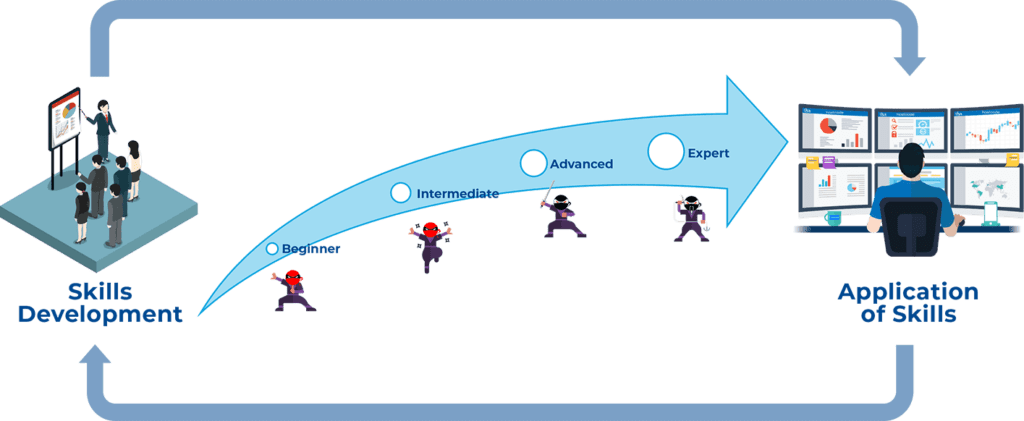
\includegraphics[width=0.95\textwidth]{images/figure 2-1.png}
	\caption{Skill Development to Application of Skills}
\end{figure}

In operational SOC environments, analysts are expected to interpret vast volumes of heterogeneous security data, including web server logs, firewall alerts, intrusion detection events, and system-level audit trails. These data sources are typically fragmented, noisy, and context dependent. Novice analysts frequently struggle to correlate isolated alerts into coherent attack narratives, resulting in delayed responses and superficial understanding.

From an educational perspective, this challenge can be abstracted as the difficulty of transforming raw, low-level security telemetry into structured, explainable knowledge that supports learning and decision-making. The proposed project conceptualizes this problem through a three-layer abstraction model:
\begin{itemize}
	\item \textbf{Security Data Generation Layer:} Simulated attack and defense activities executed within isolated Cyber Range environments.
	\item \textbf{Security Data Aggregation and Correlation Layer:} Centralized logging, Web Application Firewall (WAF), reverse proxy, and SIEM components responsible for collecting and correlating events.
	\item \textbf{Intelligent Assistance Layer:} Large Language Models used to analyze correlated events and provide natural-language explanations, insights, and guidance.
\end{itemize}

\subsection{Project Overview}

\subsubsection{The Current Situation}
In recent years, hands-on, scenario-based cybersecurity training has become an essential requirement for both educational institutions and professional training programs. Despite this shift, many existing training environments continue to exhibit several persistent limitations. First, the volume of logs and alerts generated in simulated attacks often overwhelms learners at the basic level. Second, most platforms offer limited real-time feedback, forcing learners to rely on instructors or post-exercise assessments to understand their mistakes. Finally, the scalability of instructor-led instruction is inherently limited, especially in large classes or self-paced learning settings.

These factors combined reduce training effectiveness and hinder the development of independent analytical skills in learners.

\subsubsection{Boundaries of the Solution}
To address the identified limitations, this project proposes the development of a Web-Based LLM-Augmented Cyber Range. In the proposed architecture, each user is provisioned with an isolated training environment, referred to as a user stack. Each user stack includes a vulnerable web application, a reverse proxy, a Web Application Firewall (WAF), and an attacker machine. All security events generated within these environments are centrally collected and processed by a Security Information and Event Management (SIEM) system.

A Large Language Model is integrated as an intelligent SOC assistant within the platform. Its primary function is to analyze selected security events and alerts, generate human-readable explanations of attack behaviors, and provide context-aware guidance on investigation and mitigation strategies. This approach transforms the Cyber Range from a passive simulation environment into an interactive, guided learning system.

\begin{figure}[H]
	\centering
	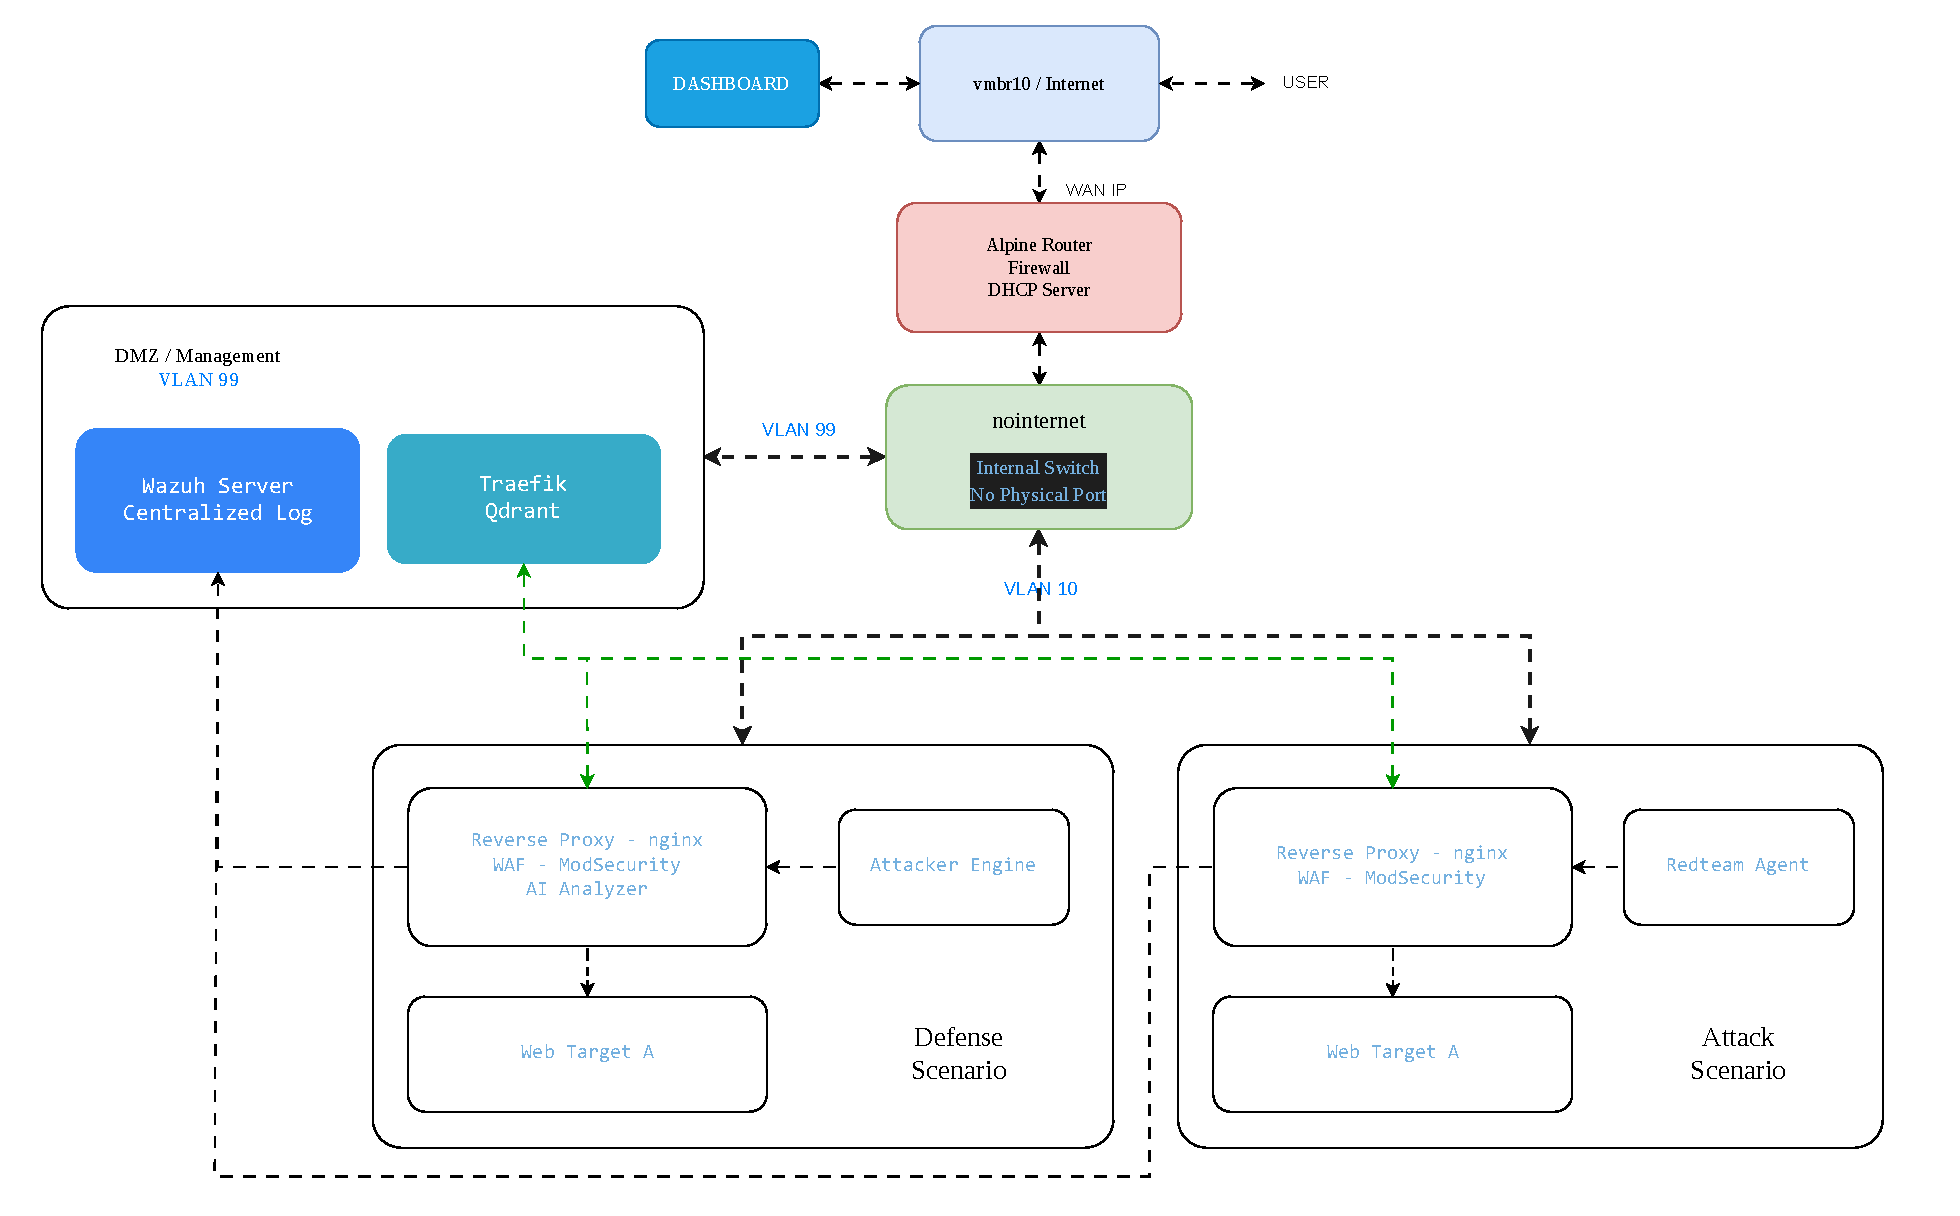
\includegraphics[width=0.95\textwidth]{images/system_flow.pdf}
	\caption{Proposed infrastructure architecture of the cyber range platform.}
	\label{fig:infra-arch}
\end{figure}

\subsubsection{Project Environment}
\begin{table}[H]
	\centering
	\begingroup
	\setlength{\tabcolsep}{3pt}
	\renewcommand{\arraystretch}{1.1}
	\small
	\begin{tabularx}{\textwidth}{|p{0.65cm}|p{2.8cm}|p{0.95cm}|p{0.95cm}|p{1.1cm}|X|p{1.45cm}|}
		\hline
		\textbf{No.} & \textbf{OS} & \textbf{CPU} & \textbf{RAM} & \textbf{Disk} & \textbf{Purpose} & \textbf{Qty.} \\
		\hline
		01 & Alpine Linux & 1 core & 0.5 GB & 4 GB & Router, Firewall, DHCP Server for internal VLAN routing and traffic control & 1 \\
		\hline
		02 & Ubuntu Server 22.04 LTS & 2 cores & 2 GB & 100 GB & Management \& DMZ node hosting Traefik Reverse Proxy, Apache Guacamole, and AI Engine services & 1 \\
		\hline
		03 & Ubuntu Server 22.04 LTS & 10 cores & 8 GB & 60 GB & Centralized SIEM server (Wazuh) for log collection, correlation, and monitoring & 1 \\
		\hline
		04 & Ubuntu Server 22.04 LTS & 4 cores & 6 GB & 30 GB & User training stack including Web Target, nginx Reverse Proxy, WAF (ModSecurity), and attacker machine & 1 per\ user \\
		\hline
		05 & Ubuntu Server 22.04 LTS & 2 cores & 2 GB & 20 GB & Additional internal services for testing, log forwarding, and system integration validation & 1 \\
		\hline
		06 & Proxmox VE Host & 13 cores & 10.5 GB & 74 GB & Virtualization host managing all virtual machines and isolated Cyber Range environments & 1 \\
		\hline
	\end{tabularx}
	\endgroup
	\caption{Development environment}
\end{table}
\FloatBarrier

\section{Project Organization}

\subsection{Solution Process Model}
The project follows an iterative and incremental development model combined with the Scrum framework. This approach was chosen to meet changing requirements, minimize technical risks from the outset, and ensure continuous validation of design decisions. Scrum allows the project team to break down complex development tasks into manageable sprints, each producing verifiable products.

At a high level, the system's operational process unfolds as follows: Users access the platform through a web-based dashboard and connect to their designated environment via Apache Guacamole, providing secure access without the need for client-side software installation. Attack and defense operations are performed in isolated user stacks, generating logs from the WAF, reverse proxy, and host operating system. These logs are aggregated and correlated by the SIEM system. The selected events are then forwarded to the LLM analysis module, which generates contextual interpretations and recommendations for the trainee.

To make implementation and validation more practical, this project also defines explicit end-to-end flow views for each major actor and subsystem. These flow views are used as technical references during development, sprint planning, and test-case design. Instead of treating the architecture only as static blocks, the team models how requests, events, and decisions move between components under normal operation and under attack-driven conditions.

The flow-oriented approach provides the following management and engineering benefits:
\begin{itemize}
\item Clarifies handoff points between infrastructure, backend services, SIEM processing, and AI analysis.
\item Makes debugging easier by identifying where delays, dropped events, or processing errors may occur.
\item Supports role assignment because each teammate can own specific flow segments and validation checkpoints.
\item Improves documentation quality by linking diagrams directly to implementation milestones.
\end{itemize}

\setlength{\LTpre}{0pt}
\setlength{\LTpost}{0pt}
\subsection{Detailed Operational Flows}
This subsection summarizes the primary flow diagrams that guide the implementation and integration process. The diagrams are organized by actor perspective and subsystem perspective so the team can validate both user behavior and platform internals.

\subsubsection{Admin Main Flow}
The admin flow focuses on environment provisioning, policy control, user-stack lifecycle, and monitoring supervision. It is used to verify that administrative operations are auditable, permission-aware, and resilient against configuration mistakes.

\begin{figure}[H]
\centering
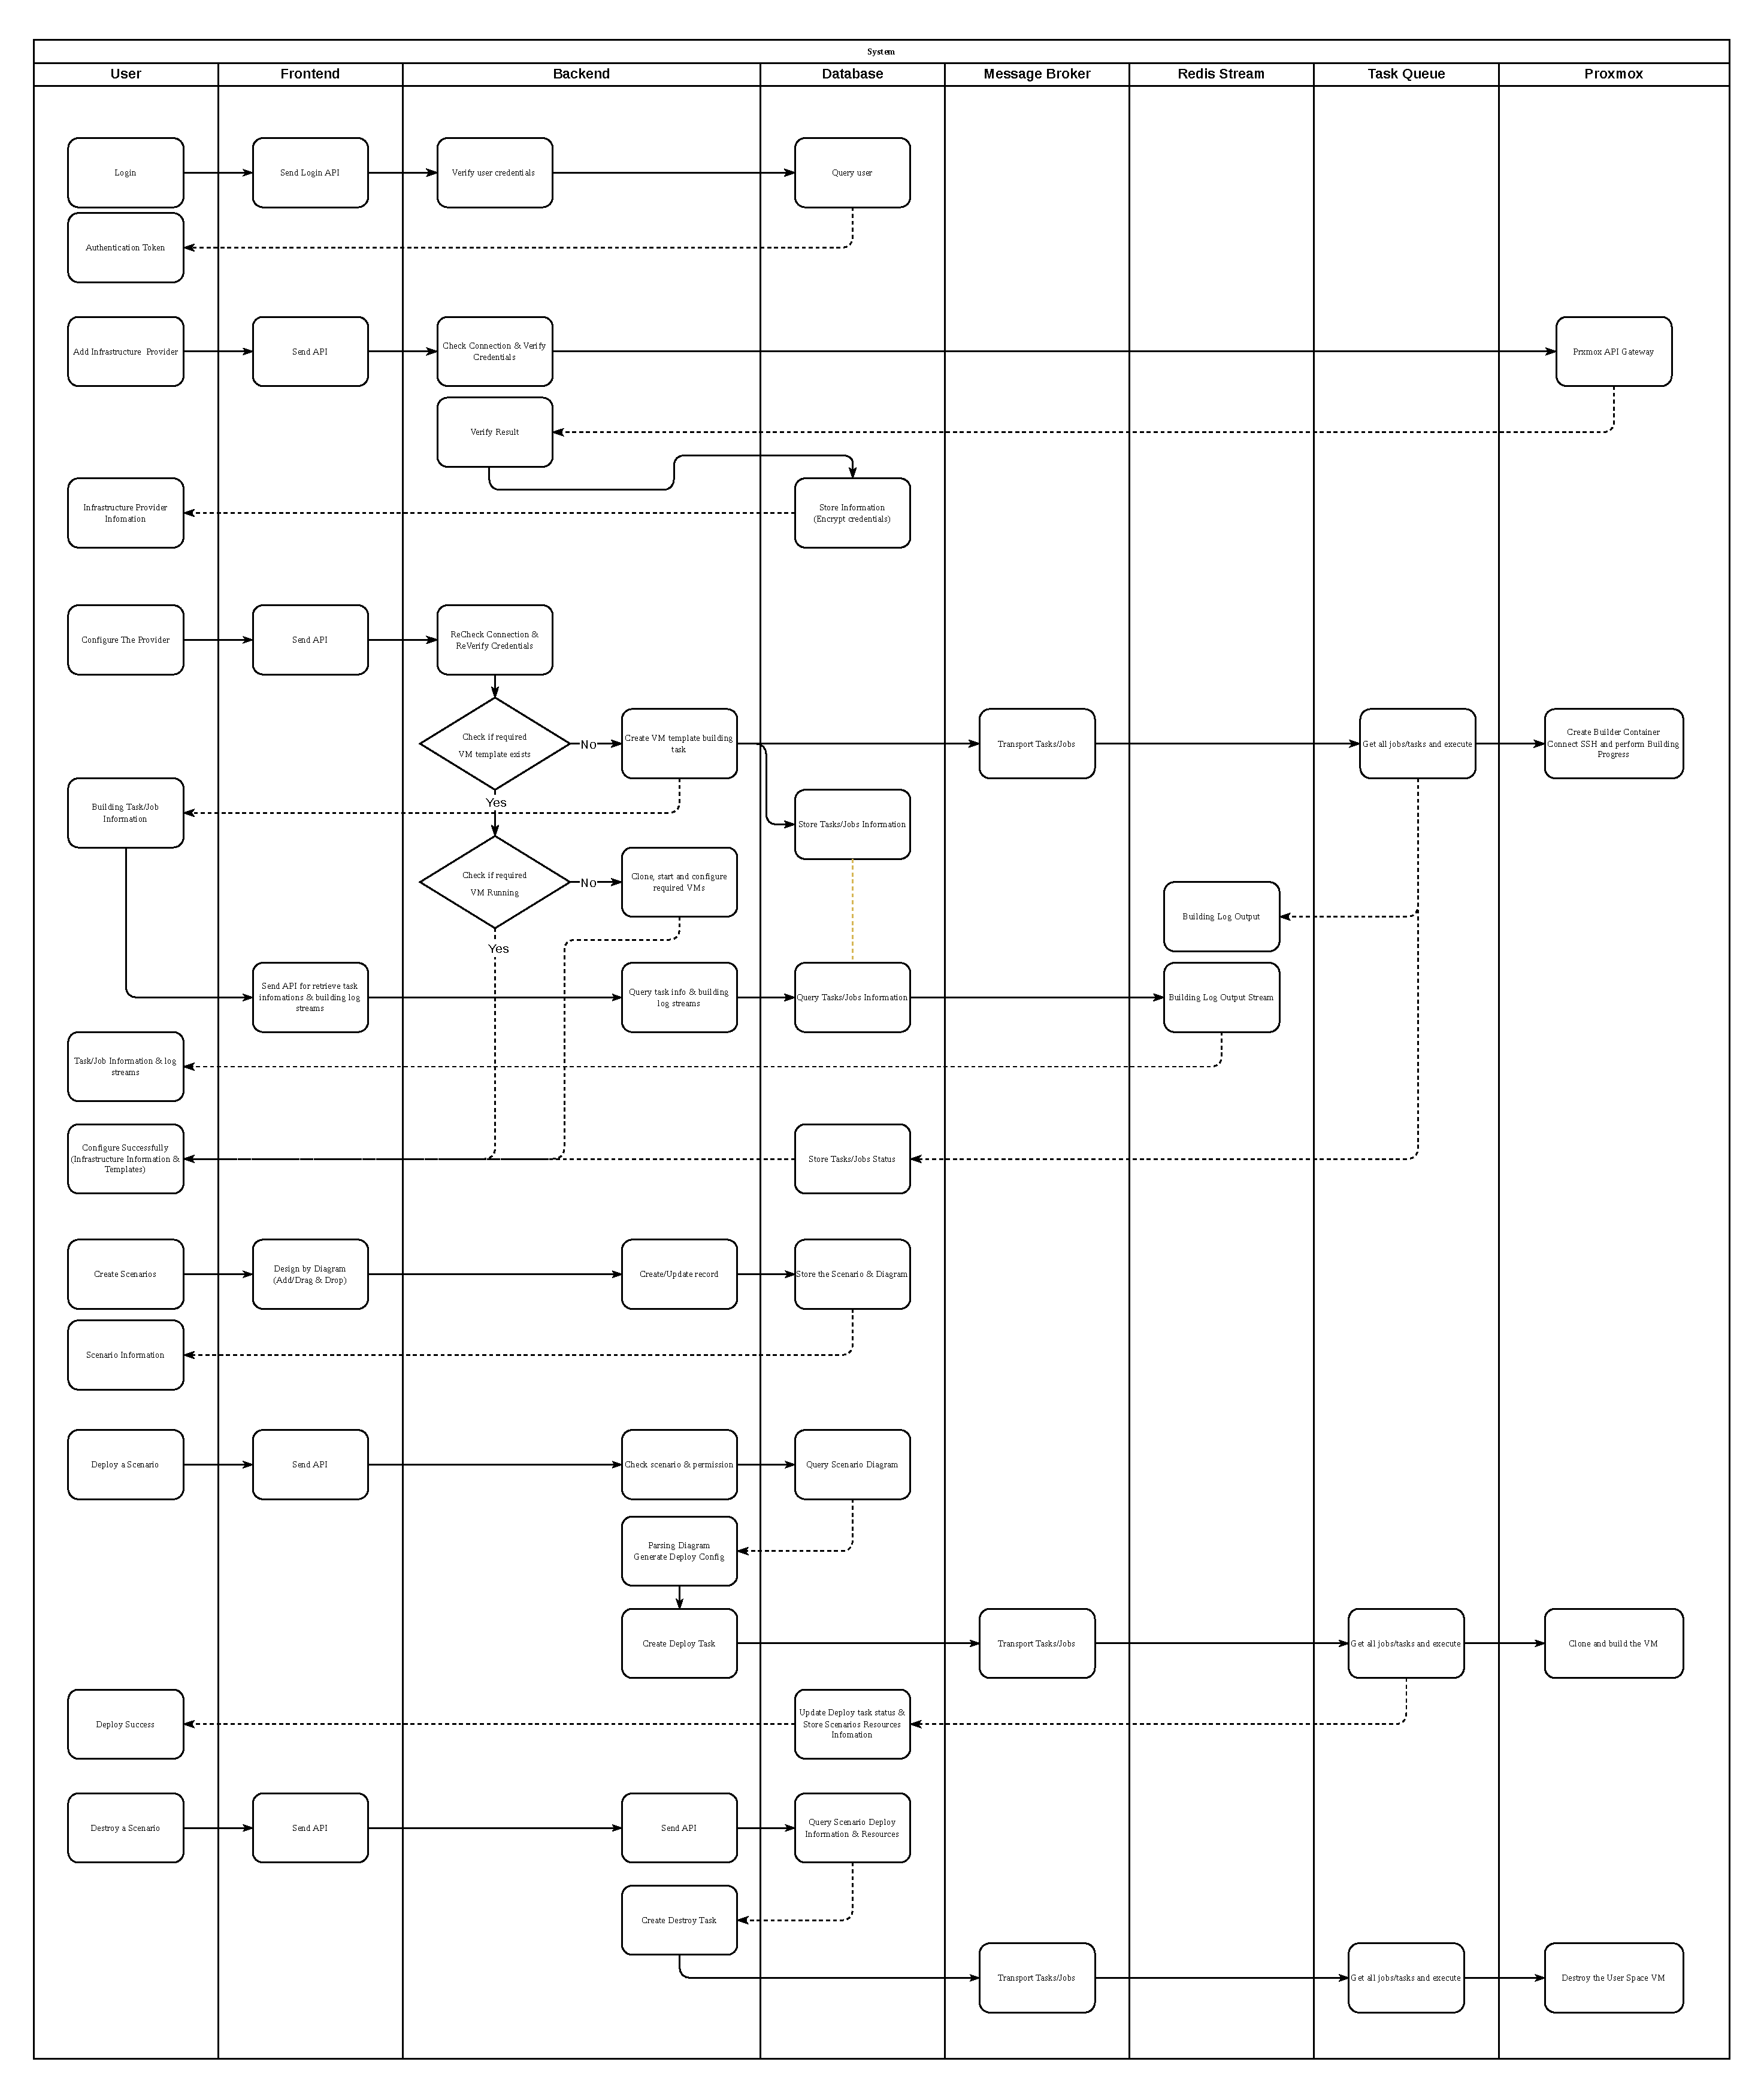
\includegraphics[width=0.95\textwidth]{images/rendered/Admin Main Flow.png}
\caption{Administrative workflow for managing cyber range operations}
\label{fig:admin-main-flow}
\end{figure}

\subsubsection{User Main Flow}
The user flow captures learner actions from login to exercise execution, alert review, and AI-assisted interpretation. This flow ensures that the training journey is coherent, measurable, and aligned with intended learning outcomes.

\begin{figure}[H]
\centering
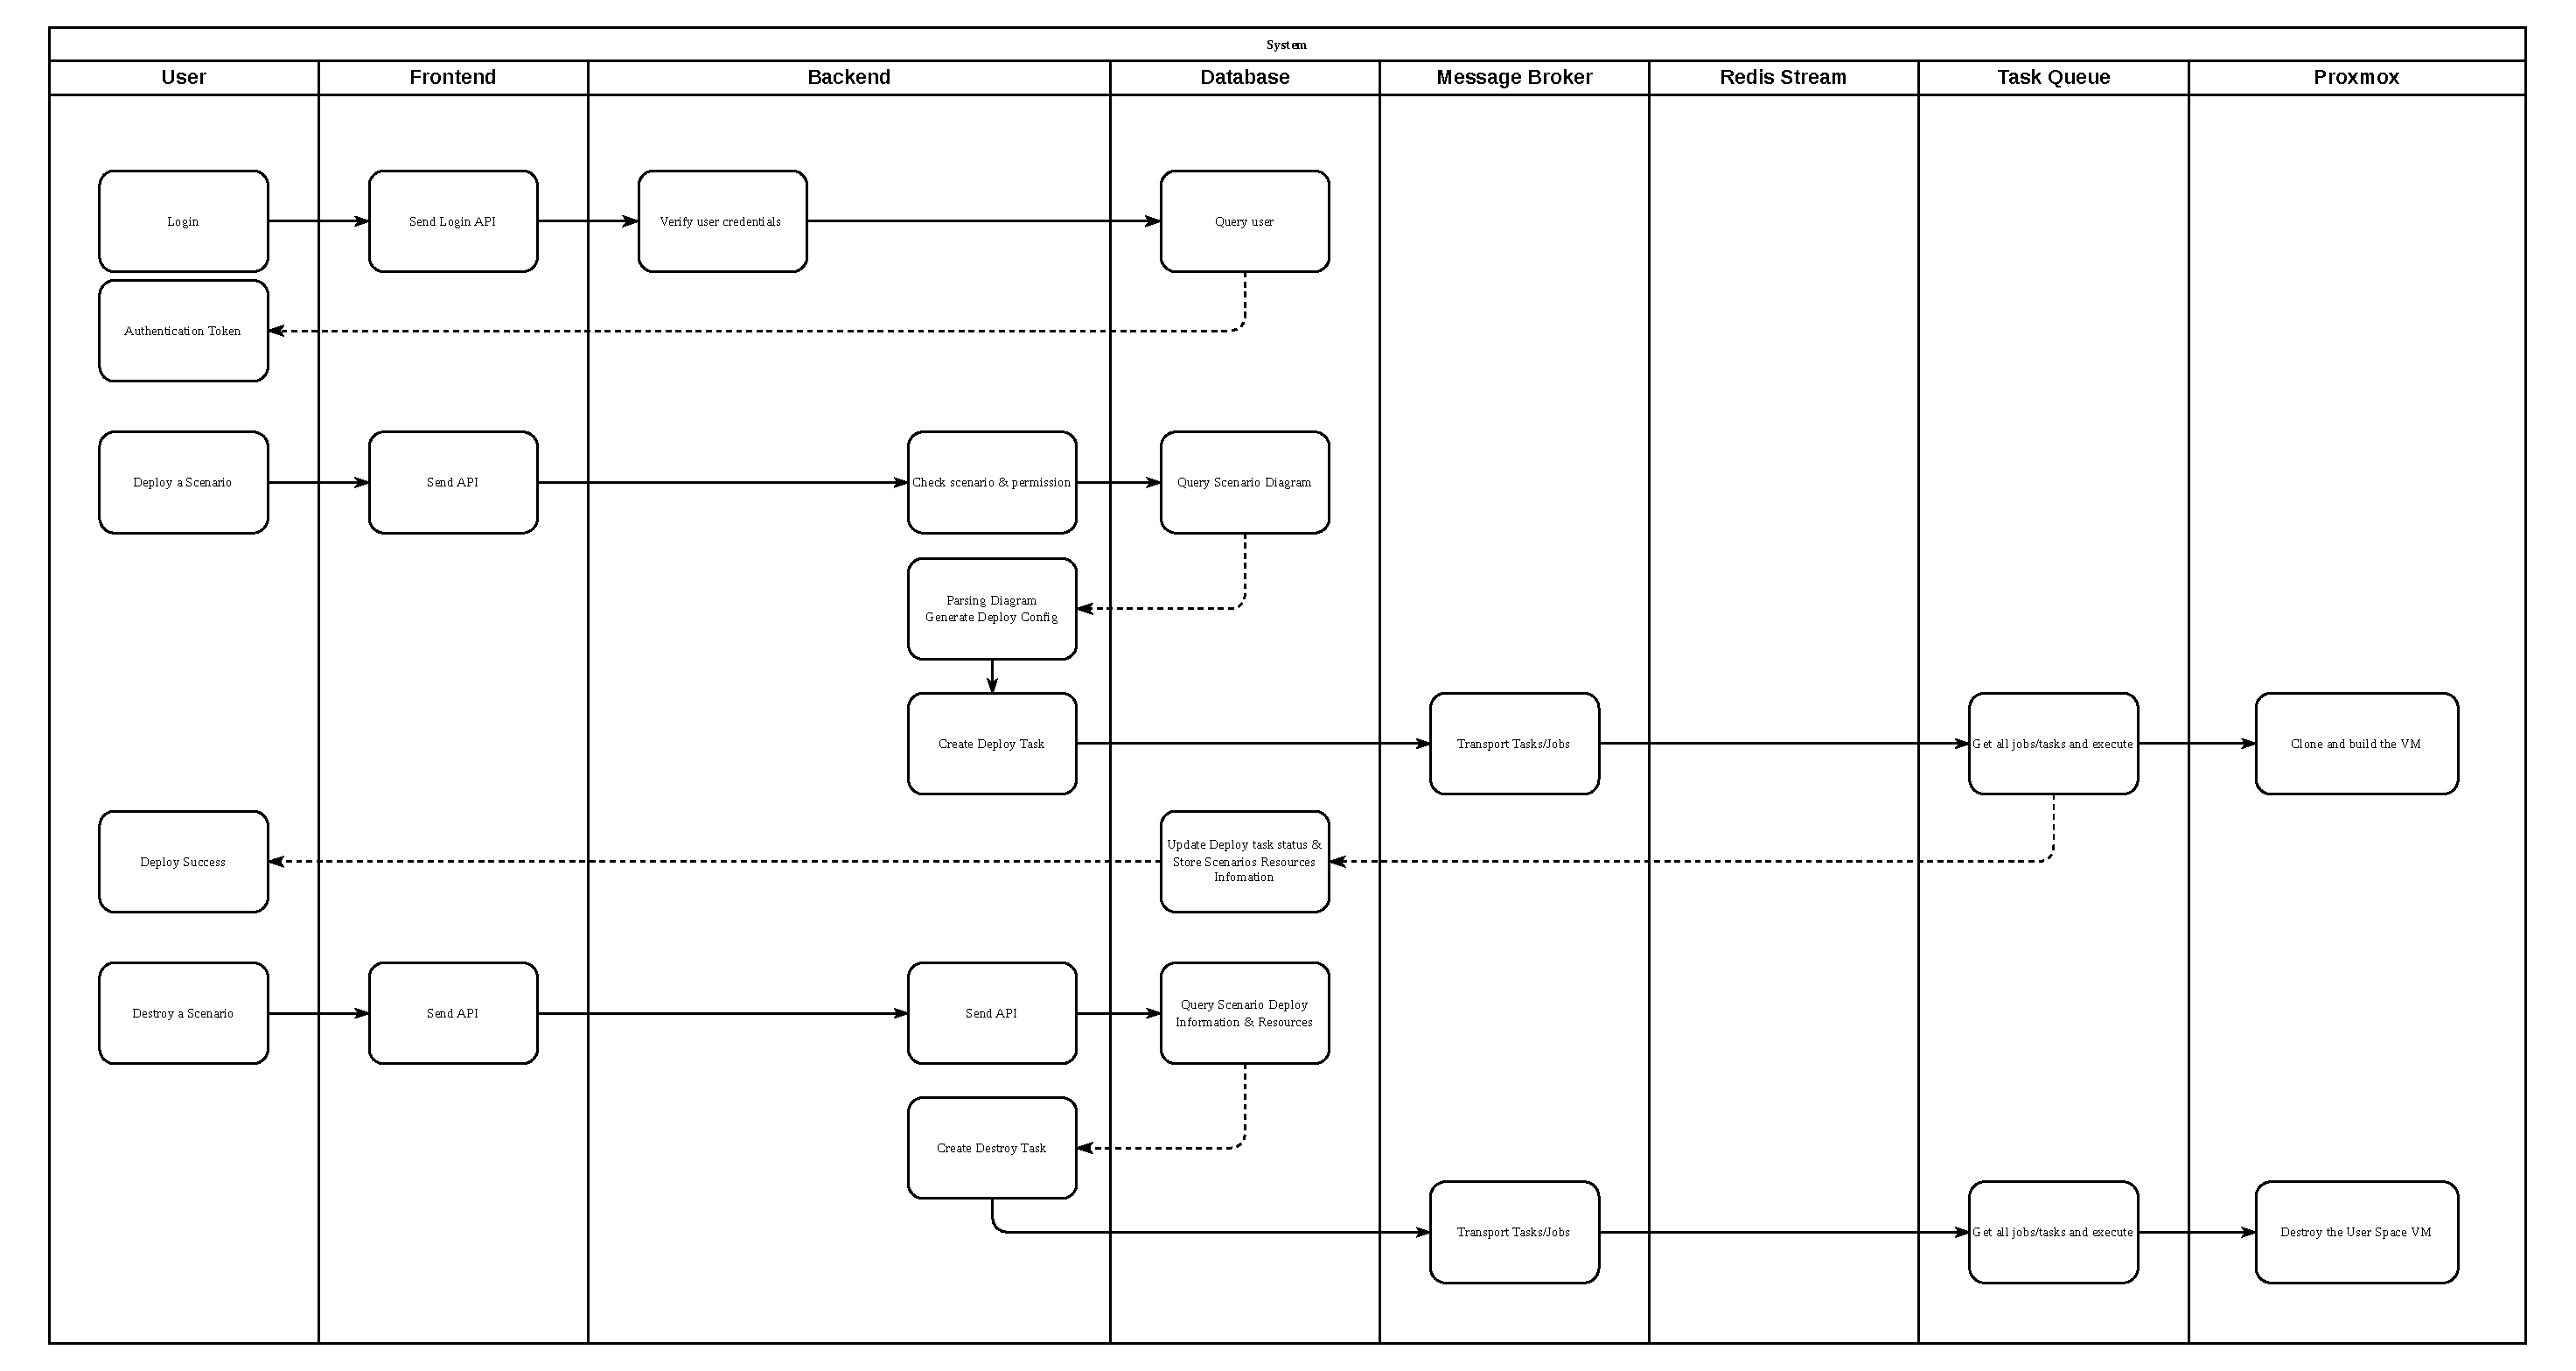
\includegraphics[width=0.95\textwidth]{images/rendered/User Main Flow.png}
\caption{Primary user interaction flow in the cyber range platform}
\label{fig:user-main-flow}
\end{figure}

\subsubsection{User Space Flow}
The user space flow describes how user-initiated actions and HTTP traffic move through the operational components of the platform, from management access to AI-assisted analysis outputs. This view emphasizes the end-to-end data path that links frontend interactions, reverse proxy monitoring, traffic replay, normalization, and service-level analysis.

In this flow, user and admin interactions first reach the management backend, which coordinates control operations and stores configuration state in the management database. Attack or training traffic then passes through the NGINX and ModSecurity layer, where request inspection and security logging are performed before logs are forwarded through Wazuh-related monitoring and HTTP ingest services.

A replay and forwarding stage is used to preserve realistic HTTP traces for backend service processing and AI analysis. The AI analyzer service receives normalized events, generates contextual interpretations, and stores results in the logs database for later review and dashboard presentation.

\begin{figure}[H]
\centering
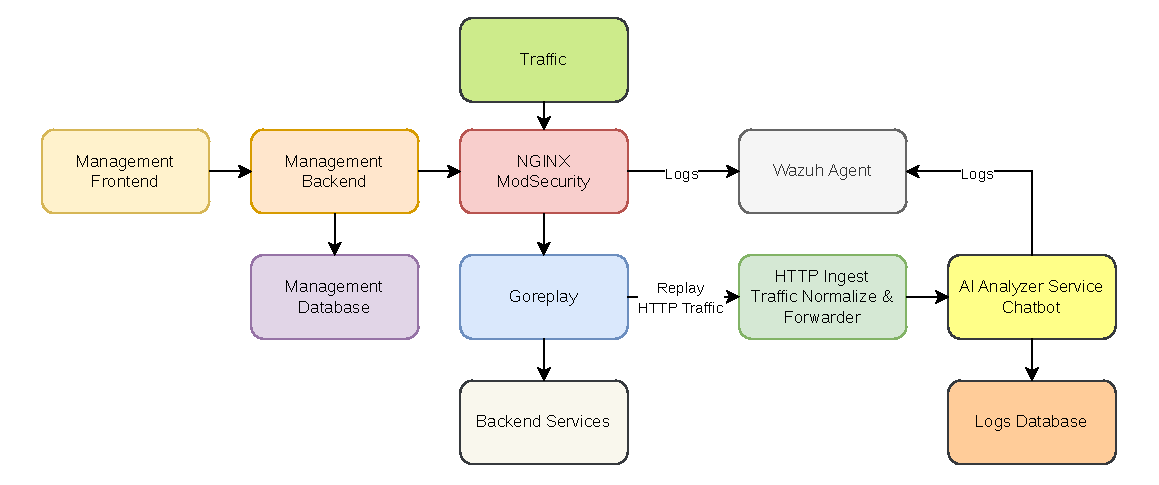
\includegraphics[width=0.95\textwidth]{images/User Space.pdf}
\caption{User space data flow across management, monitoring, and AI analysis}
\label{fig:user-space-flow}
\end{figure}

\subsubsection{User Use Case Flow}
The user use case flow defines the major functional interactions between platform actors and scenario-management capabilities. The diagram shows two primary actors (Admin and User), where the Admin performs full lifecycle operations and the User performs scenario participation and resource access actions.

Core use cases include login, viewing scenarios, accessing resources, and managing scenario execution. Administrative capabilities additionally include scenario design, system settings configuration, infrastructure provider management, user-role management, and controlled teardown of scenario runs.

This use-case perspective complements the system-flow diagrams by clarifying functional permissions, helping the team design role-based access control policies and prioritize feature implementation according to actor responsibility.

\begin{figure}[H]
\centering
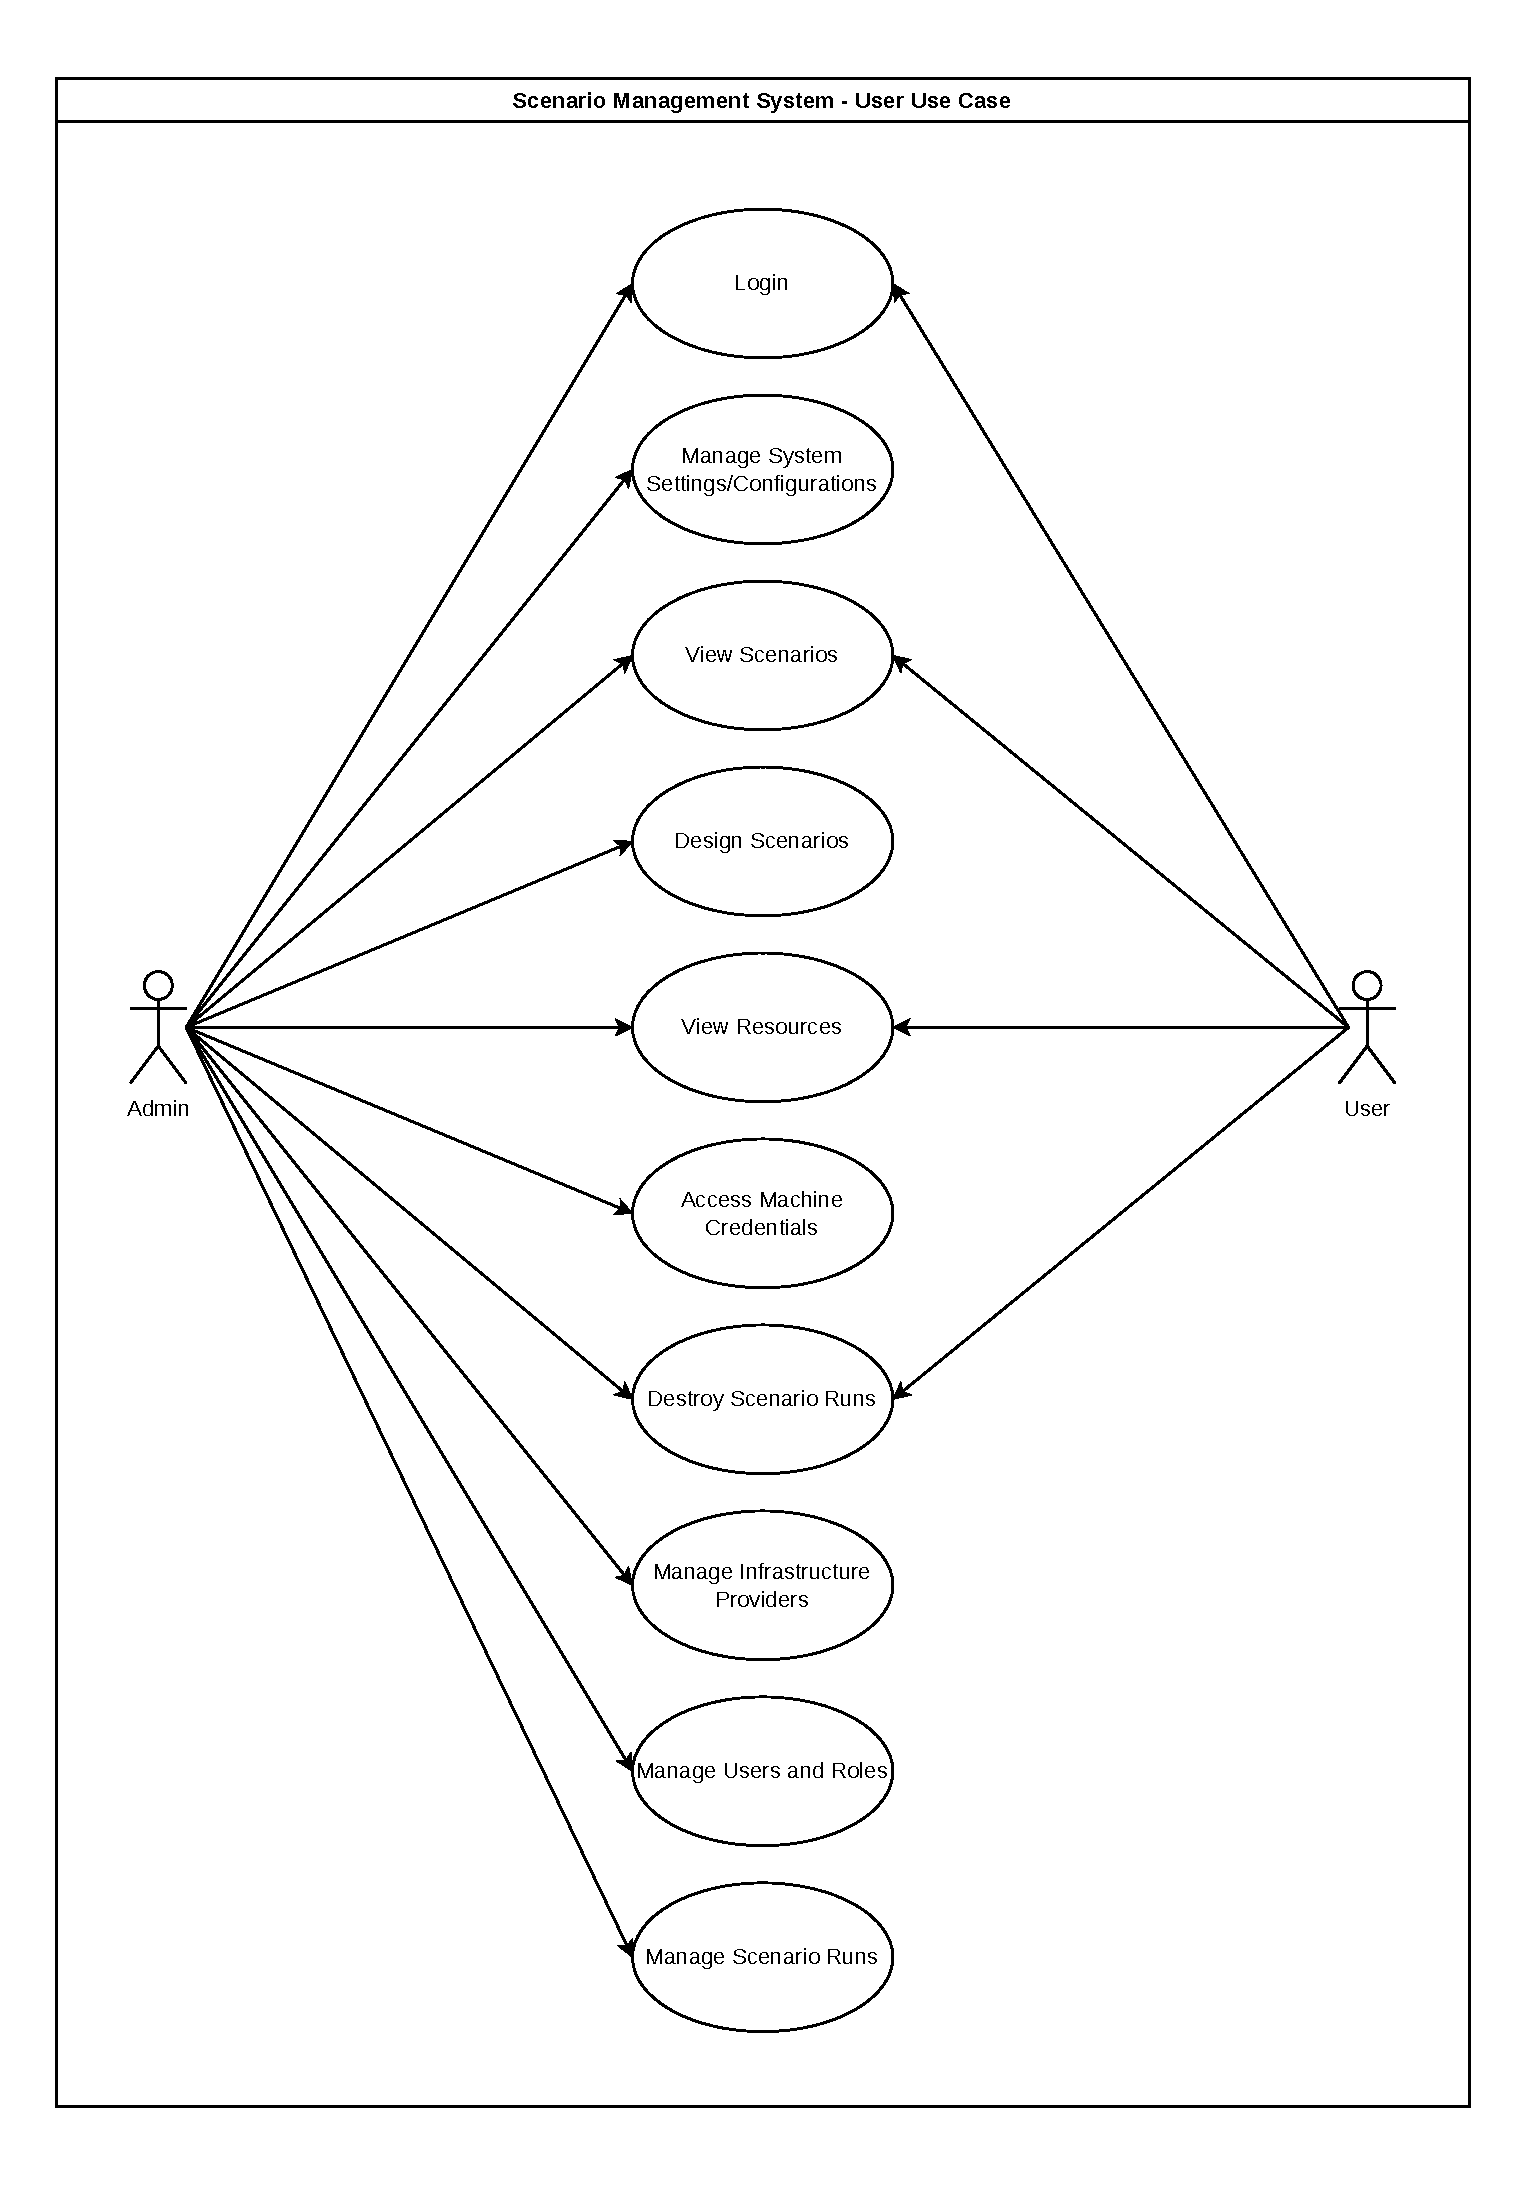
\includegraphics[width=0.95\textwidth]{images/rendered/User Use Case.png}
\caption{User and admin use-case interactions in the scenario management subsystem}
\label{fig:user-use-case-flow}
\end{figure}

\subsubsection{Blue Team Agent Flow}
The Blue Team agent flow describes how logs are ingested, normalized, correlated, and escalated for AI interpretation. This flow is important for validating response latency and consistency of detection outputs.

\begin{figure}[H]
\centering
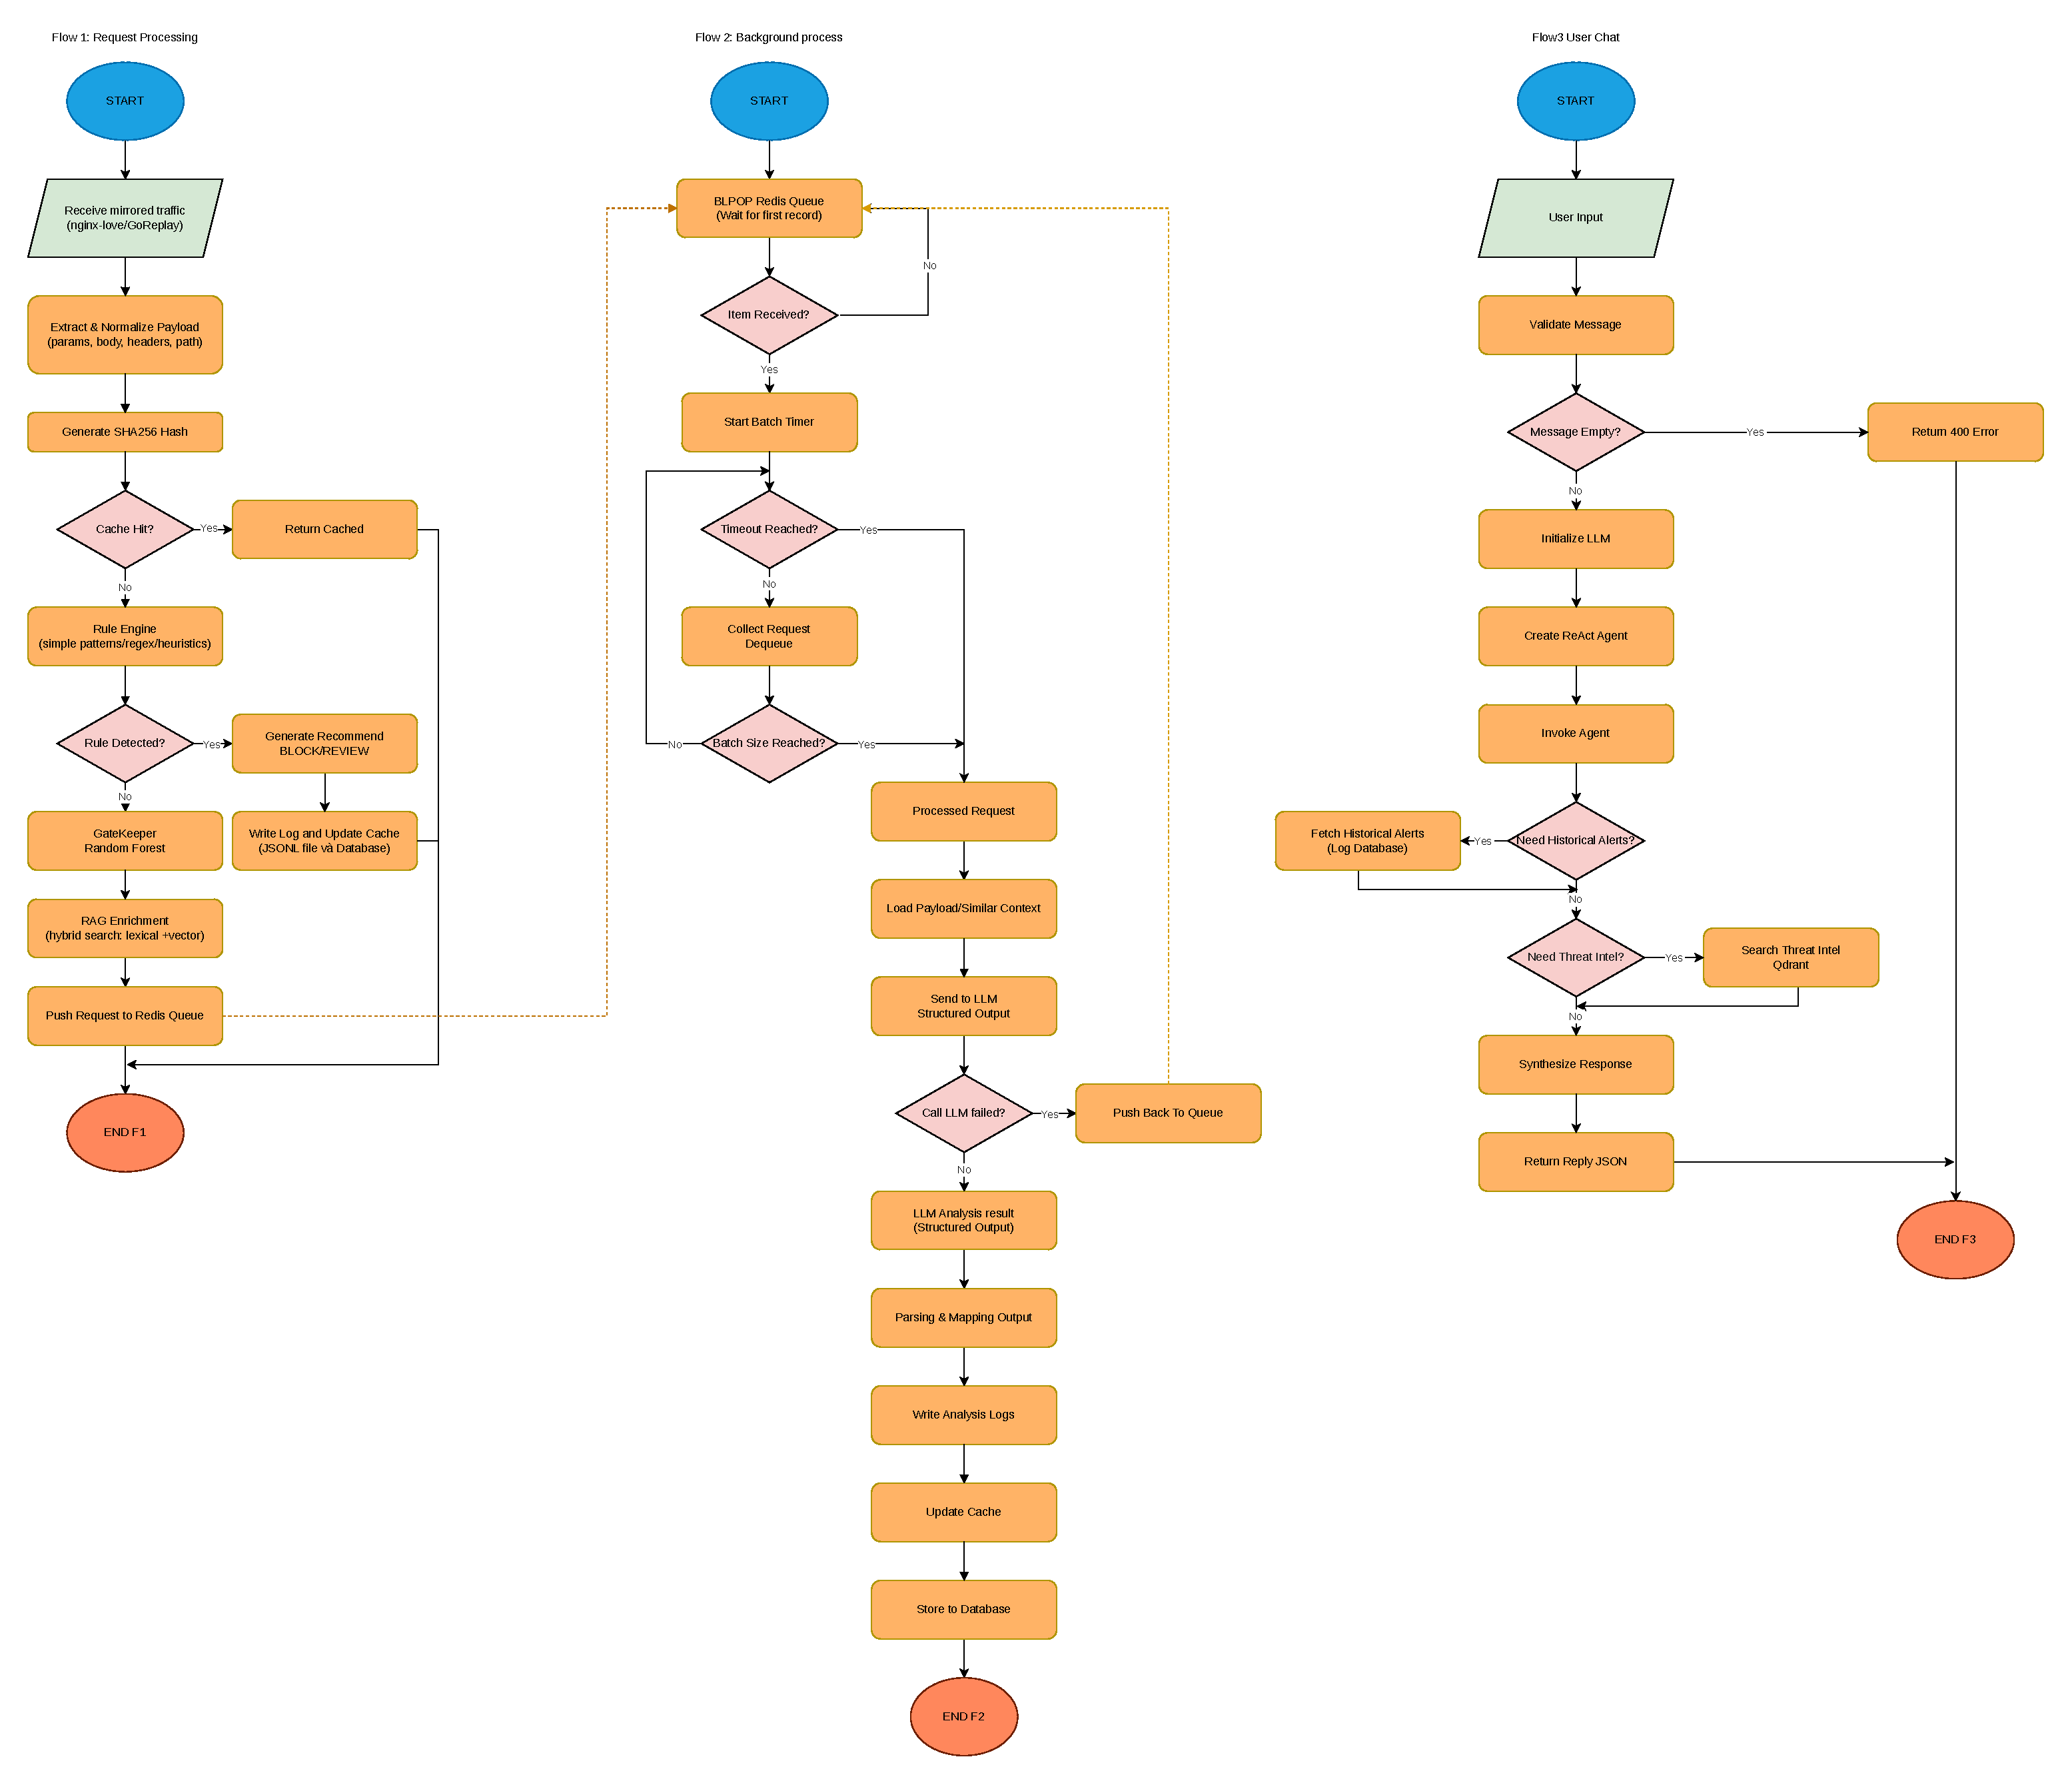
\includegraphics[width=0.95\textwidth]{images/Blueteam_Agent.pdf}
\caption{Blue Team analysis and response pipeline flow}
\label{fig:blueteam-flow}
\end{figure}

\subsubsection{Dashboard Component Flow}
The dashboard component flow explains how frontend modules consume backend endpoints, render alert intelligence, and display AI recommendations. This view is used to coordinate backend contract design and frontend state handling.

\begin{figure}[H]
\centering
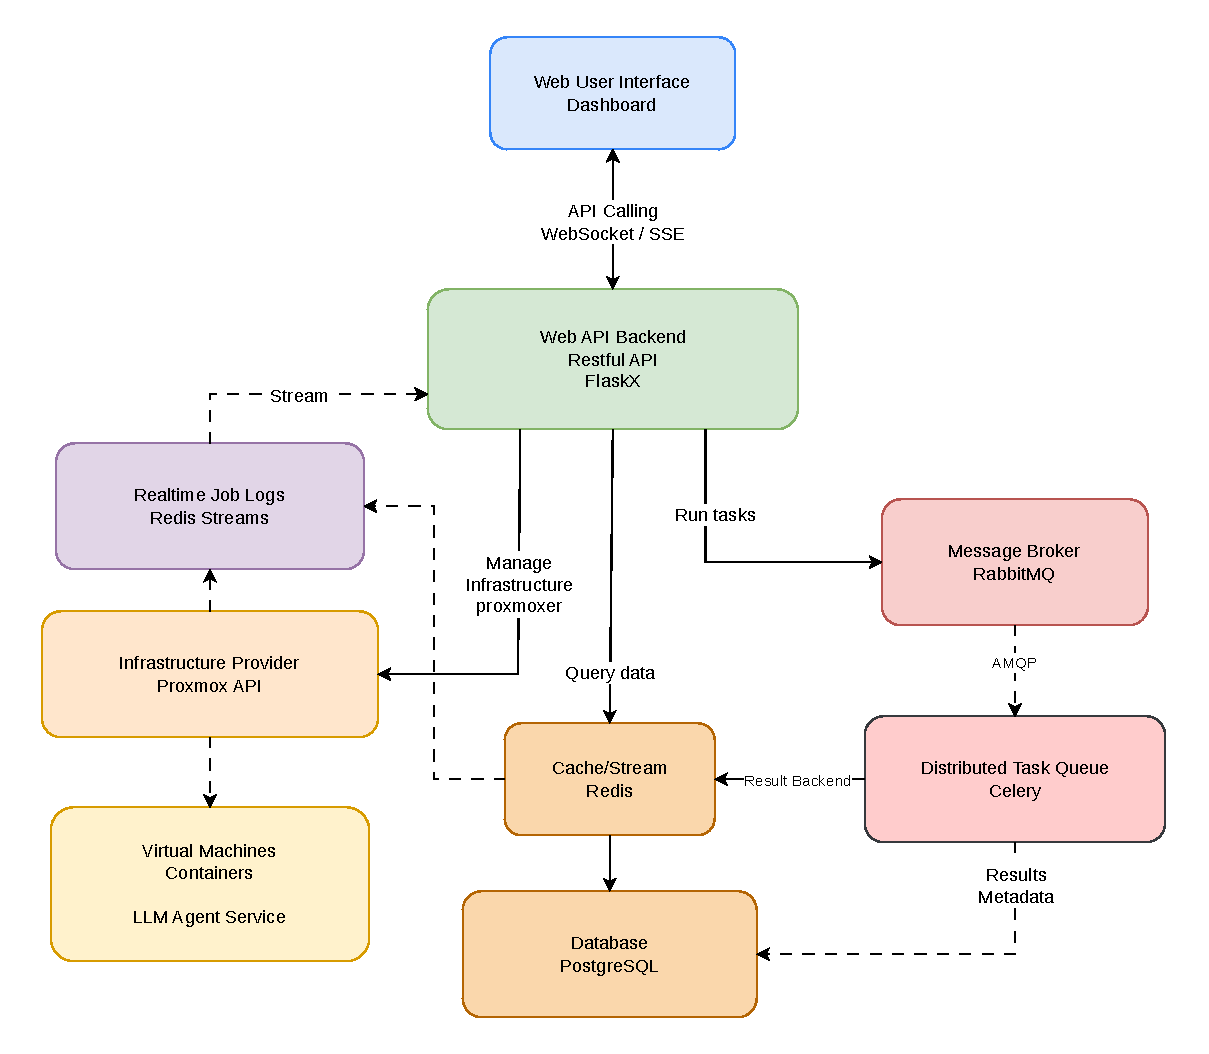
\includegraphics[width=0.95\textwidth]{images/Dashboard.pdf}
\caption{Dashboard component interaction flow for monitoring and analysis}
\label{fig:dashboard-flow}
\end{figure}

\clearpage
\subsection{Roles and Responsibilities}
\begingroup
\setlength{\LTleft}{\fill}
\setlength{\LTright}{\fill}
\setlength{\tabcolsep}{3pt}
\renewcommand{\arraystretch}{1.2}
\small
\begin{longtable}{|p{2.5cm}|p{3.0cm}|p{2.8cm}|p{5.2cm}|}
	\hline
	\textbf{Phase} & \textbf{Full Name} & \textbf{Role} & \textbf{Responsibility} \\
	\hline
	\endfirsthead
	\hline
	\textbf{Phase} & \textbf{Full Name} & \textbf{Role} & \textbf{Responsibility} \\
	\hline
	\endhead

	Initiating & Huỳnh Ngọc Quang & Project Leader & Define project objectives, scope, and overall research direction. Propose the system architecture for the LLM-augmented Cyber Range. Coordinate initial discussions with the supervisor and align technical goals with academic requirements. \\
	\hline
	Initiating & Nguyễn Văn Nhân & Infrastructure Architect & Analyze infrastructure requirements and design the virtualized Cyber Range environment. Define VLAN segmentation, routing strategy, and core services including SIEM, WAF, and reverse proxy. \\
	\hline
	Initiating & Trương Mỹ Vy & AI Researcher & Conduct background research on Large Language Models and their applications in cybersecurity education. Identify feasible LLM use cases for automated security analysis and training assistance. \\
	\hline
	Initiating & Hồ Tài Liên Vy Kha & AI Building and Documentation Coordinator & Conduct initial research on the application of LLMs in cybersecurity training environments. Prepare the initial project proposal, outline report structure, and ensure compliance with capstone documentation standards. \\
	\hline
	Planning & Huỳnh Ngọc Quang & Project Leader & Decompose project objectives into detailed sprint-level tasks and milestones. Define technical deliverables, evaluation criteria, and integration checkpoints. Coordinate planning activities to ensure alignment between infrastructure, AI research, and documentation workstreams. \\
	\hline
	Planning & Nguyễn Văn Nhân & Infrastructure Engineer & Design the detailed infrastructure deployment plan, including Proxmox virtualization layout, VLAN segmentation, routing strategy, and resource allocation. Plan scalability for multi-user Cyber Range environments and ensure isolation between user stacks. \\
	\hline
	Planning & Trương Mỹ Vy & AI Researcher & Design the AI-assisted security analysis workflow, focusing on how security events and logs are transformed into structured inputs for LLM processing. Define research hypotheses related to AI effectiveness in cybersecurity training. \\
	\hline
	Planning & Hồ Tài Liên Vy Kha & AI Building and Documentation Coordinator & Plan the AI implementation architecture using the LangGraph framework for LLM orchestration. Design the AI interaction flow between SIEM outputs and the web-based dashboard. Prepare detailed documentation outlines and reporting templates. \\
	\hline
	Executing & Huỳnh Ngọc Quang & Infrastructure Engineer & Oversee system implementation progress and coordinate integration between infrastructure components, AI services, and the dashboard. Validate intermediate deliverables and ensure adherence to the planned timeline. \\
	\hline
	Executing & Nguyễn Văn Nhân & Infrastructure Engineer & Deploy and configure Cyber Range infrastructure components, including the Alpine-based router, DMZ services, SIEM server, reverse proxies, WAF, and isolated user stacks. Ensure network stability, secure access, and proper log forwarding. \\
	\hline
	Executing & Trương Mỹ Vy & AI Researcher & Conduct experimental evaluation of AI-assisted security analysis. Test different prompt strategies and analyze the quality, accuracy, and usefulness of LLM-generated explanations within training scenarios. \\
	\hline
	Executing & Hồ Tài Liên Vy Kha & AI Building and Documentation Coordinator & Implement AI pipelines using the LangGraph framework to orchestrate LLM workflows. Integrate AI-generated outputs into the web-based user interface. Continuously update technical documentation based on implementation progress. \\
	\hline
	Deployment & Huỳnh Ngọc Quang & Project Leader & Coordinate system deployment and conduct end-to-end integration validation. Prepare demonstration scenarios and training use cases for evaluation and project defense. \\
	\hline
	Deployment & Nguyễn Văn Nhân & Infrastructure Engineer & Optimize system performance, validate VLAN isolation, and ensure secure clientless access through Apache Guacamole. Monitor system stability under simulated user load. \\
	\hline
	Deployment & Trương Mỹ Vy & AI Researcher & Evaluate the effectiveness of AI-assisted analysis in realistic training scenarios. Identify limitations, failure cases, and opportunities for improvement in AI explanations. \\
	\hline
	Deployment & Hồ Tài Liên Vy Kha & AI Building and Documentation Coordinator & Validate the integration between the LangGraph-based AI workflows and the frontend dashboard. Conduct usability testing to ensure AI outputs are clearly presented and understandable for trainees. \\
	\hline
	Closing & Huỳnh Ngọc Quang & Project Leader & Compile the final project report, summarize technical and research outcomes, and coordinate final presentation and defense activities. \\
	\hline
	Closing & Nguyễn Văn Nhân & Infrastructure Engineer & Support final system verification and assisyt in technical explanation during project evaluation and defense. \\
	\hline
	Closing & Trương Mỹ Vy & AI Researcher & Document research findings, experimental results, and identified limitations of AI-assisted security analysis. Propose future research directions, including autonomous AI attacker extensions. \\
	\hline
	Closing & Hồ Tài Liên Vy Kha & AI Building and Documentation Coordinator & Finalize system documentation, AI workflow descriptions (LangGraph-based), and user guides. Ensure consistency between implemented features and academic deliverables. \\
	\hline
	\caption{Team role and responsibilities each phase} \\
\end{longtable}

\subsection{Tools and Techniques}
\renewcommand{\arraystretch}{1.2}
\begin{longtable}{|p{0.7cm}|p{2.8cm}|p{2.8cm}|p{2.0cm}|p{4.7cm}|}
	\hline
	\textbf{No.} & \textbf{Tools} & \textbf{Category} & \textbf{Version} & \textbf{Description} \\
	\hline
	\endfirsthead
	\hline
	\textbf{No.} & \textbf{Tools} & \textbf{Category} & \textbf{Version} & \textbf{Description} \\
	\hline
	\endhead
	01 & Proxmox VE & Virtualization Platform & 8.x & Used as the core virtualization layer to provision, isolate, and manage virtual machines and containers for Cyber Range scenarios. It supports snapshot-based recovery, resource allocation control, and repeatable lab orchestration for multiple users. \\
	\hline
	02 & Ubuntu Server & Operating System & 22.04 LTS & Primary server operating system for SIEM, management, and integration services. Chosen for long-term stability, security patch support, broad package compatibility, and operational reliability in capstone deployment conditions. \\
	\hline
	03 & Alpine Linux & Operating System & 3.x & Lightweight distribution used for router and firewall functions where minimal footprint and reduced attack surface are required. It improves efficiency for network control services such as DHCP, NAT, and segmentation routing. \\
	\hline
	04 & Docker & Containers & 24.x & Provides consistent runtime environments for application and middleware components. Docker simplifies packaging, deployment repeatability, dependency isolation, and rapid rollback when validating attack-defense workflows. \\
	\hline
	05 & Traefik & Reverse Proxy & 2.x & Deployed as an edge ingress layer in the DMZ for traffic routing and service exposure control. It helps centralize request forwarding policies, supports secure entrypoint management, and improves maintainability for multi-service architecture. \\
	\hline
	06 & Nginx & Web Server / Reverse Proxy & 1.24.x & Used in user stacks to proxy traffic to vulnerable applications and to provide logging points for security analysis. Nginx acts as a key telemetry source when combined with ModSecurity and SIEM correlation rules. \\
	\hline
	07 & ModSecurity & Web Application Firewall & 3.x & Provides inspection and filtering for HTTP traffic to detect common web attacks, including SQL Injection and Cross-Site Scripting patterns. It supports rule-driven enforcement and contributes high-value security events to the monitoring pipeline. \\
	\hline
	08 & Wazuh & SIEM Platform & 4.x & Centralized platform for log ingestion, normalization, rule correlation, and alert visualization. Wazuh serves as the SOC analysis backbone and provides the structured event context consumed by AI and dashboard workflows. \\
	\hline
	09 & Apache Guacamole & Remote Access Gateway & 1.5.x & Enables browser-based, clientless access to isolated training machines via protocols such as SSH and RDP. This improves usability for trainees while preserving centralized access control and network boundary protection. \\
	\hline
	10 & LangGraph & LLM Orchestration Framework & 1.0.9 & Implements graph-based orchestration for multi-step AI reasoning. LangGraph is used to model explicit state transitions, tool invocation flow, fallback branches, and response assembly so that security explanations remain structured, traceable, and operationally controllable. \\
	\hline
	11 & Gemini API & LLM Inference API & API-based & Provides the language-model inference layer for natural-language analysis of correlated events. In this project, Gemini-backed workflows are used to generate attack interpretation, investigation hints, and mitigation-oriented explanations suitable for trainee comprehension. \\
	\hline
	12 & FastAPI & API Backend Framework & Latest stable & Serves as the integration backbone connecting SIEM outputs, rule-based preprocessing, retrieval modules, and LangGraph workflows. FastAPI endpoints handle request validation, asynchronous processing, structured responses, and API-level error handling for dashboard consumption. \\
	\hline
	13 & Qdrant & Vector Database & Latest stable & Stores and indexes dense vectors representing security knowledge, historical incidents, and contextual references. Qdrant enables semantic retrieval to enrich AI prompts with relevant context and reduce hallucination risk in generated explanations. \\
	\hline
	14 & HuggingFace Embeddings & Embedding Model Provider & Model-dependent & Converts logs, alerts, and security reference text into vector representations for similarity search. These embeddings support Retrieval-Augmented Generation by supplying targeted context to LLM workflows before response generation. \\
	\hline
	15 & OWASP CRS-style Regex Engine & Rule-based Detection Engine & Custom ruleset & Applies deterministic pattern matching inspired by OWASP Core Rule Set logic to flag known web attack signatures, suspicious payload structures, and anomalous request indicators. It functions as a fast first-pass detection layer before advanced AI analysis. \\
	\hline
	16 & Python & Programming Language & 3.10 & Main implementation language for backend services, orchestration glue code, log preprocessing utilities, evaluation scripts, and automation tasks across the full attack-defense training pipeline. \\
	\hline
	17 & Git & Version Control & Latest & Used for source management, branch-based collaboration, review workflows, and change traceability across infrastructure scripts, backend services, AI workflow definitions, and report artifacts. Git also supports rollback and auditability during iterative sprint delivery. \\
	\hline
	18 & JavaScript & Frontend Development & ES6+ & Used to build interactive dashboard components for lab control, alert visualization, and AI explanation display. JavaScript enables responsive user experience and real-time interaction between trainees and backend services. \\
	\hline
	19 & HTML5 / CSS3 & Frontend Technologies & HTML5 / CSS3 & Provides semantic structure and visual styling for the web interface. These technologies are used to ensure readability, accessibility, and consistent presentation of monitoring and AI-assisted analysis outputs. \\
	\hline
		20 & Custom Training Web Application & Web Application Test Target & Project build & Self-developed web application used to reproduce web attack scenarios such as SQL Injection, XSS, and request manipulation inside the cyber range. This target reflects the project-specific deployment model and provides controlled validation for monitoring and AI-assisted analysis workflows. \\
		\hline
		21 & Custom Containerized Web Stack & Containerized Application Stack & Project build & Containerized web services developed and deployed by the project team to validate scenario orchestration, reverse-proxy inspection, attack logging, and runtime access workflows. This stack is used instead of public training applications so that experiments remain aligned with the designed scenario architecture. \\
		\hline
	\caption{Tools and techniques used in project.} \\
\end{longtable}
\endgroup

\subsection{Retrieval-Augmented Generation for Security Analysis}
Retrieval-Augmented Generation (RAG) is adopted in this project to improve the factual grounding and contextual relevance of AI-generated security explanations. Instead of sending raw alerts directly to the language model, the system first retrieves related knowledge from an indexed security knowledge base and then injects that context into the final prompt. This design is particularly suitable for cyber range training because the same alert may require different interpretations depending on HTTP payloads, WAF signatures, attack stages, and previously observed evidence.

In the proposed platform, the RAG mechanism acts as an intermediate reasoning support layer between SIEM outputs and the Gemini-based analysis module. The retrieval stage reduces ambiguity by attaching semantically relevant references, such as attack descriptions, known payload patterns, rule explanations, and prior incident context, before the response generation step is executed. As a result, the AI assistant is better aligned with the monitored events and less likely to generate vague or hallucinated explanations.

\begin{figure}[H]
	\centering
	
\includegraphics[width=0.9\textwidth]{images/RAG_pic.png}
	\caption{RAG workflow in the proposed platform.}
	\label{fig:rag-workflow}
\end{figure}

The operational logic of the RAG module in this project consists of five main stages. First, structured events are collected from the monitoring pipeline, including WAF alerts, HTTP request traces, rule metadata, and analyst-selected context. Second, these inputs are normalized and converted into a compact query representation suitable for semantic search. Third, the query is embedded and compared against indexed security knowledge stored in Qdrant. Fourth, the most relevant retrieved items are combined with the current alert evidence to form an augmented prompt. Finally, Gemini generates an explanation that is grounded in both observed runtime evidence and retrieved background knowledge.

From an implementation perspective, the RAG workflow complements the LangGraph orchestration layer. LangGraph controls when retrieval is required, how many supporting references should be attached, and how fallback behavior should be handled when the retrieved context is weak or incomplete. This makes the AI pipeline more traceable and more suitable for instructional use, because each answer can be explained as the result of a staged process rather than a single opaque LLM response.

\subsubsection{RAG Processing Logic}
The RAG workflow used in the capstone can be summarized as follows:

\begin{enumerate}
	\item \textbf{Event intake:} Receive selected SIEM alerts, HTTP logs, ModSecurity messages, and user-provided investigation context from the platform.
	\item \textbf{Normalization:} Extract key fields such as request path, parameters, matched rules, suspicious payload fragments, timestamps, and severity level.
	\item \textbf{Query formulation:} Transform the normalized evidence into a concise retrieval query that represents the current security problem.
	\item \textbf{Vector embedding:} Encode the query using the embedding model so that semantic similarity search can be performed.
	\item \textbf{Knowledge retrieval:} Search Qdrant for the top-k most relevant knowledge chunks, including attack descriptions, defensive guidance, and historical references.
	\item \textbf{Context augmentation:} Merge the retrieved knowledge with the original alert evidence to construct a grounded AI prompt.
	\item \textbf{LLM generation:} Submit the augmented prompt to Gemini to produce a human-readable explanation, likely attack interpretation, and suggested response actions.
	\item \textbf{Result presentation:} Return the generated explanation to the dashboard for trainee review and further investigation.
\end{enumerate}

\subsubsection{Algorithmic Description}
The following algorithm summarizes the logical sequence used by the proposed RAG-enabled security assistant.

\noindent\textbf{Algorithm 1: RAG-based security event analysis}

\begin{enumerate}
	\item \textbf{Input:} Correlated security event set $E$, indexed knowledge base $K$, embedding model $M$, vector database $V$, language model $L$.
	\item Parse $E$ to extract the main indicators of compromise, suspicious request features, matched WAF rules, and alert metadata.
	\item Normalize the extracted evidence into a structured analysis object $A$.
	\item Generate a retrieval query $Q$ from $A$.
	\item Encode $Q$ using $M$ to obtain the query vector $q$.
	\item Search $V$ over knowledge base $K$ using $q$ and retrieve the top-k relevant documents $D = \{d_1, d_2, ..., d_k\}$.
	\item Rank or filter $D$ to remove weak or redundant context segments.
	\item Construct an augmented prompt $P$ by combining $A$ with the retained retrieved knowledge.
	\item Submit $P$ to language model $L$ to generate response $R$.
	\item \textbf{Output:} Return $R$ as the final contextual explanation, investigation guidance, and mitigation-oriented suggestion.
\end{enumerate}

This algorithm is intentionally designed for cybersecurity education rather than fully autonomous incident response. The primary goal is not only to classify attacks, but also to explain why an event is suspicious, what evidence supports the interpretation, and what investigation or mitigation steps should be considered next. Therefore, the RAG layer serves both an accuracy function and a pedagogical function inside the web-based cyber range.

\section{Project Management Plan}

\subsection{Tasks}
The project can be divided into several major phases, each further decomposed into a set of minor tasks and distributed across multiple development sprints. Each sprint represents an intensive work cycle aimed at delivering specific outcomes, thereby ensuring steady progress, effective coordination, and continuous validation throughout the project lifecycle.

\subsubsection{Sprint 01: Requirements Analysis and Initial System Design}
During this sprint, the team focuses on gathering, analyzing, and formalizing the project requirements. The objective is to establish a solid conceptual and technical foundation for the LLM-augmented Cyber Range. This sprint emphasizes understanding the attack surface, defining training objectives, and designing the initial system architecture.

The responsibilities in this sprint include the following:
\begin{itemize}
	\item Collecting and documenting functional and non-functional requirements for the Cyber Range platform.
	\item Analyzing the target attack surface and defining the scope of web-based attack and defense scenarios.
	\item Designing the high-level system architecture, including virtualization, network segmentation, SIEM integration, and AI-assisted analysis components.
	\item Selecting core tools and technologies such as Proxmox, Docker, Wazuh, ModSecurity, Apache Guacamole, and the LangGraph framework for LLM orchestration.
	\item Preparing initial architectural diagrams and validating the design with the project supervisor.
\end{itemize}

\subsubsection{Sprint 02: Infrastructure Deployment and Network Configuration}
The second sprint focuses on deploying the foundational infrastructure of the Cyber Range environment. This sprint translates the architectural design into a functional virtualized system capable of supporting isolated training environments.

The responsibilities in this sprint include the following:
\begin{itemize}
	\item Deploying the Proxmox virtualization platform and provisioning virtual machines and containers.
	\item Configuring VLAN-based network segmentation to isolate management, user stacks, and internal services.
	\item Deploying and configuring the Alpine-based router, including firewall rules and DHCP services.
	\item Setting up the DMZ environment and internal switching components.
	\item Configuring secure clientless access using Apache Guacamole.
	\item Verifying network isolation, routing correctness, and controlled internet access.
\end{itemize}

\subsubsection{Sprint 03: Security Services Integration and Log Management}
Sprint 03 focuses on integrating security mechanisms and centralized log management into the Cyber Range. The goal of this sprint is to generate realistic security events and establish a SOC-style monitoring pipeline.

The responsibilities in this sprint include the following:
\begin{itemize}
		\item Deploying self-developed web applications within isolated user stacks to generate controlled attack and monitoring data.
	\item Configuring nginx as a reverse proxy and integrating ModSecurity as a Web Application Firewall.
	\item Executing controlled attack and defense scenarios to generate security logs.
	\item Deploying and configuring the Wazuh SIEM platform for centralized log collection, normalization, and correlation.
	\item Creating alert rules and dashboards to support security monitoring and analysis.
	\item Validating the end-to-end log flow from user stacks to the SIEM system.
\end{itemize}

\subsubsection{Sprint 04: LLM Integration and AI-Assisted Security Analysis}
Sprint 04 is dedicated to integrating artificial intelligence into the Cyber Range. This sprint introduces LLM-based analysis to transform raw security data into contextual, human-readable insights for training purposes.

The responsibilities in this sprint include the following:
\begin{itemize}
	\item Designing AI workflows using the LangGraph framework to orchestrate Large Language Model interactions.
	\item Defining structured inputs for AI analysis based on SIEM alerts, HTTP requests, and correlated security events.
	\item Implementing retrieval-augmented prompting so AI explanations remain grounded in relevant security knowledge.
	\item Integrating AI-generated outputs into the BlueAgent WAF Console and related web-based dashboard views.
	\item Evaluating the accuracy, relevance, and usefulness of AI-assisted explanations in training scenarios.
	\item Refining AI interaction logic based on experimental feedback.
\end{itemize}

\subsubsection{Sprint 05: System Validation, Evaluation, and Documentation}
The final sprint focuses on validating the complete system, evaluating its effectiveness, and finalizing project documentation. This sprint ensures that all components operate cohesively and that project outcomes are clearly documented.

The responsibilities in this sprint include the following:
\begin{itemize}
	\item Conducting end-to-end system testing across infrastructure, security services, AI modules, and the user interface.
	\item Evaluating system performance, stability, and usability under simulated training conditions.
	\item Assessing the effectiveness of AI-assisted analysis in supporting cybersecurity training.
	\item Finalizing technical documentation, system descriptions, and experimental results.
	\item Documenting system limitations and proposing future enhancements, including autonomous AI-driven attacker modules.
	\item Preparing the final report and materials for project presentation and defense.
\end{itemize}

\subsection{Task Sheet: Assignments and Timetable}
\begingroup
\setlength{\LTleft}{\fill}
\setlength{\LTright}{\fill}
\setlength{\tabcolsep}{3pt}
\renewcommand{\arraystretch}{1.1}
\small
\begin{longtable}{|p{3.0cm}|p{2.4cm}|p{1.9cm}|p{1.6cm}|p{4.4cm}|}
	\hline
	\textbf{Task} & \textbf{Assigned To} & \textbf{Estimated Duration} & \textbf{Deadline} & \textbf{Description} \\
	\hline
	\endfirsthead
	\hline
	\textbf{Task} & \textbf{Assigned To} & \textbf{Estimated Duration} & \textbf{Deadline} & \textbf{Description} \\
	\hline
	\endhead
	\hline
	\multicolumn{5}{r}{\textit{Continued on next page}} \\
	\endfoot
	\endlastfoot
	Project planning and scope definition & Huỳnh Ngọc Quang & 1 week & Week 1 & Define project objectives, scope, deliverables, and success criteria for the CyberRange system. \\
	\hline
	CyberRange environment setup & Nguyễn Văn Nhân & 2 weeks & Weeks 2 & Deploy isolated CyberRange stacks including vulnerable web applications and supporting services. \\
	\hline
	Research on web attack patterns & Trương Mỹ Vy & 1 week & Weeks 2 & Study common web attacks (SQLi, XSS, LFI, SSRF, etc.) and their characteristics in HTTP logs. \\
	\hline
	AI preprocessing module development & Hồ Tài Liên Vy Kha & 2 weeks & Week 2 & Implement multi-layer preprocessing logic to classify attacks and reduce LLM invocation. \\
	\hline
	System architecture design & Huỳnh Ngọc Quang & 1 week & Week 3 & Design the overall CyberRange architecture, including attacker, defender, WAF, SIEM, Dashboard and AI workflow components. \\
	\hline
	WAF and reverse proxy configuration & Nguyễn Văn Nhân & 1 week & Week 3 & Configure ModSecurity and reverse proxy to inspect and filter incoming HTTP traffic. \\
	\hline
	AI detection methodology design & Trương Mỹ Vy & 1 week & Week 3 & Propose AI-based detection approaches combining rule-based, heuristic, and LLM-assisted analysis. \\
	\hline
	LLM integration and workflow implementation & Hồ Tài Liên Vy Kha & 1 week & Week 3 & Integrate LLM into the analysis pipeline for handling uncertain or complex attack cases. \\
	\hline
	Risk management and progress tracking & Huỳnh Ngọc Quang & Continuous & Project-wide & Identify project risks, track progress, and adjust plans to ensure project stability. \\
	\hline
	Attack simulation environment & Nguyễn Văn Nhân & 1 week & Week 4 & Set up attacker machines and tools to generate realistic attack traffic for testing. \\
	\hline
	Attack-Defense evaluation metrics & Trương Mỹ Vy & 1 week & Week 5 & Define metrics to measure success of AI attacks versus AI defenses. \\
	\hline
	Attack-Defense feedback loop & Hồ Tài Liên Vy Kha & 1 week & Week 6 & Integrate attack results as feedback to refine defensive AI rules and logic. \\
	\hline
	Final integration review and validation & Huỳnh Ngọc Quang & 1 week & Week 7 & Validate system integration, ensure all components work cohesively, and prepare for final defense. \\
	\hline
	Infrastructure optimization and stability testing & Nguyễn Văn Nhân & 1 week & Week 8 & Optimize performance, ensure isolation between users, and maintain system stability. \\
	\hline
	AI workflow improvement suggestions & Trương Mỹ Vy & Continuous & Project-wide & Propose improvements to reduce unnecessary LLM usage while maintaining accuracy. \\
	\hline
	Documentation of attack scenarios & Hồ Tài Liên Vy Kha & Continuous & Project-wide & Document attack strategies, payloads, and evaluation results in the final report. \\
	\hline
	\caption{Assignment task sheet} \\
\end{longtable}
\endgroup

\subsection{Meeting Minutes}
\begin{table}[!htbp]
	\centering
	\begingroup
	\small
	\setlength{\tabcolsep}{4pt}
	\renewcommand{\arraystretch}{1.1}
	\begin{tabularx}{\textwidth}{|p{3.2cm}|X|}
		\hline
		\textbf{Subject} & SP26IA01 \\
		\hline
		\textbf{Instructor} & Mr. Mai Hoàng Đỉnh \\
		\hline
		\textbf{Location} & FPT HCM Campus\\
		\hline
		\textbf{Attendees} & Huỳnh Ngọc Quang (SE181838), Nguyễn Văn Nhân (SE183547), Trương Mỹ Vy (SE184728), Hồ Tài Liên Vy Kha (SE173290) \\
		\hline
		\textbf{Absence} &  \\
		\hline
		\textbf{Date} & 01/2026 -- 4/2026 \\
		\hline
		\textbf{Time} & 09:30 A.M -- 11:30 A.M every Monday \\
		\hline
	\end{tabularx}
	\caption{Meeting minute}
	\endgroup
\end{table}
	% !TeX root = ../main.tex
\chapter{RISK MANAGEMENT}

\section{The Essentials of Risk Assessment}
Risk management is a critical component in the development and deployment of cybersecurity systems. In complex environments such as cyber range platforms, which simulate real-world attack and defense scenarios, the system architecture involves multiple interacting components including virtualized infrastructure, traffic monitoring systems, distributed processing pipelines, and artificial intelligence-based analysis engines. Each of these components introduces potential security, operational, and reliability risks that must be carefully assessed.

In the context of this capstone project, the proposed system integrates Large Language Models (LLMs) into a web-based cyber range platform to support automated analysis of security events and web traffic logs. The system captures HTTP requests generated from simulated cyberattack scenarios and processes them through a multi-stage analysis pipeline. The pipeline includes request normalization, rule-based detection, asynchronous task processing, and contextual interpretation using LLMs.

While this architecture provides powerful capabilities for automated security analysis and cybersecurity training, it also introduces potential risks associated with distributed processing systems, infrastructure misconfiguration, and AI-assisted decision making. If these risks are not properly managed, they may lead to system failures, inaccurate analysis results, or exposure of sensitive information.

Therefore, implementing a structured risk management framework is essential to ensure that the cyber range platform remains secure, reliable, and suitable for educational purposes.

The risk management process in this project aims to:
\begin{itemize}
    \item Identify potential security threats and vulnerabilities within the system architecture;
    \item Evaluate the likelihood and potential impact of these risks;
    \item Prioritize risks based on severity and operational impact;
    \item Propose mitigation strategies to reduce or eliminate identified risks.
\end{itemize}

By performing a comprehensive risk assessment, the development team can proactively address system weaknesses before deployment and ensure that the training environment remains safe for experimentation.

\subsection{Purpose and Objectives of Risk Assessment}
The purpose of risk assessment in this project is to establish a structured framework for identifying, analyzing, and mitigating potential risks that may affect the operation of the LLM-assisted cyber range platform.

Unlike traditional web applications, cyber range environments are designed to simulate real cyberattack scenarios. This means that the platform intentionally processes malicious traffic, attack payloads, and abnormal system behaviors generated during training exercises. As a result, the system must be carefully designed to ensure that simulated attacks remain confined within the training infrastructure and do not affect other components of the platform.

Furthermore, the integration of artificial intelligence into the analysis pipeline introduces additional challenges. While LLMs can provide valuable insights and explanations for security events, they may also produce inaccurate interpretations if the input data is incomplete or ambiguous. Therefore, risk assessment must consider both infrastructure-level risks and AI-related risks.

The objectives of the risk assessment process include:

\begin{itemize}
    \item \textbf{Identifying Security Threats:} The system processes web traffic logs generated from simulated attacks. These logs may contain malicious payloads such as SQL injection strings, command injection attempts, or cross-site scripting scripts. Improper handling of these payloads could expose vulnerabilities in the log processing system.

    \item \textbf{Evaluating Infrastructure Reliability:} The platform relies on distributed processing using message queues and worker nodes. If the queue becomes overloaded or worker nodes fail, the system may experience delays in processing security logs.

    \item \textbf{Protecting Sensitive Data:} Security logs, training data, and analysis results represent valuable information that must be protected from unauthorized access or tampering.

    \item \textbf{Ensuring Reliability of AI-assisted Analysis:} The LLM component plays an important role in generating explanations and recommendations for security events. Incorrect interpretations or model errors may affect the accuracy of training outcomes.
\end{itemize}

By addressing these objectives, the risk assessment framework ensures that the system can operate safely while supporting realistic cybersecurity training scenarios.

\subsection{Risk Assessment Process}
The risk assessment process for this project follows several stages commonly used in cybersecurity risk management frameworks.

These stages include risk identification, risk estimation, risk prioritization, and control implementation.

\subsubsection{Risk Identification}
The first step in the risk assessment process involves identifying potential risks that may arise within the cyber range platform. This process examines both the system architecture and operational workflows of the platform.

The architecture includes several major components:
\begin{itemize}
    \item Virtualized cyber range infrastructure;
    \item Traffic monitoring and log collection mechanisms;
    \item Backend API services;
    \item Distributed task processing systems;
    \item LLM-based analysis modules;
    \item Centralized logging and storage systems.
\end{itemize}
Each component may introduce potential risks such as misconfiguration, unauthorized access, or system performance issues.

\subsubsection{Risk Estimation}
After identifying potential risks, the next step is to evaluate the likelihood of each risk and the severity of its potential impact.

Likelihood represents the probability that a risk will occur during system operation, while impact represents the severity of consequences if the risk occurs.

For example:
\begin{itemize}
    \item Misconfigured API endpoints may have a relatively high likelihood due to development complexity.
    \item Failures in external AI services may have medium likelihood depending on network stability.
    \item Hardware failures may have low likelihood but high impact if they occur.
\end{itemize}
Estimating both likelihood and impact allows the development team to better understand the relative severity of each risk.

\subsubsection{Risk Prioritization}
Once risks have been estimated, they are categorized based on their severity.

Three main risk levels are used in this project:

\begin{itemize}
    \item \textbf{High Risk:} High risk issues have both high likelihood and high impact. These risks must be addressed immediately before system deployment.
    \item \textbf{Medium Risk:} Medium risk issues have moderate likelihood or moderate impact. These risks should be monitored and mitigated progressively.
    \item \textbf{Low Risk:} Low risk issues have minimal impact and can be addressed later as part of system maintenance.
\end{itemize}

Prioritizing risks in this manner helps ensure that development resources are allocated effectively.

\subsection{System Architecture Overview and Security Considerations}
The cyber range platform proposed in this project follows a modular architecture designed to support realistic cybersecurity training scenarios. The system integrates infrastructure virtualization, traffic monitoring mechanisms, and AI-assisted analysis services.

The architecture consists of several layers including:
\begin{itemize}
    \item User interaction layer;
    \item Application backend layer;
    \item Distributed task processing layer;
    \item Infrastructure orchestration layer;
    \item Virtualized training environment layer.
\end{itemize}
Each layer plays a specific role in enabling the cyber range platform to capture, process, and analyze simulated attack traffic.

Because the system processes potentially malicious inputs generated during training exercises, it must be designed with strong security controls and isolation mechanisms.

\subsubsection{Cyber Range Infrastructure Layer}
The cyber range infrastructure layer provides the foundation for the training platform. It consists of virtual machines and containers that simulate real-world IT environments.

The infrastructure is managed using a virtualization platform such as Proxmox, which enables dynamic provisioning of training environments.

Each training environment is organized into an isolated \textbf{user stack}, which typically includes:
\begin{itemize}
    \item An attacker machine used for launching simulated attacks;
    \item A vulnerable target system;
    \item Monitoring and analysis components.
\end{itemize}
This isolation ensures that activities performed by one trainee do not affect other users.

However, the use of virtualization introduces potential risks such as resource exhaustion, network misconfiguration, and unauthorized access between virtual machines.

\subsubsection{Traffic Monitoring Layer}
The system captures web traffic generated during training exercises using a reverse proxy traffic mirroring mechanism.

The reverse proxy intercepts HTTP requests before forwarding them to target web applications. At the same time, it records request metadata such as:
\begin{itemize}
    \item HTTP method;
    \item Request URL;
    \item Headers;
    \item Payload data.
\end{itemize}
These logs are then forwarded to the centralized analysis pipeline.

Because the reverse proxy processes raw user input, improper handling of HTTP payloads may introduce vulnerabilities such as injection attacks targeting the log processing system.

\subsubsection{Application Backend and AI Analysis Layer}
The application backend coordinates communication between different system components.

The backend is implemented as a RESTful API using Flask and serves as the central control component for the platform.

Its responsibilities include:
\begin{itemize}
    \item Managing training environments;
    \item Retrieving analysis results;
    \item Initiating analysis tasks;
    \item Communicating with the dashboard interface.
\end{itemize}
The backend interacts with the LLM analysis service to interpret security logs and generate contextual explanations for detected attack patterns.

The LLM can identify patterns such as SQL injection attempts, directory traversal attacks, and authentication bypass attempts.

However, the integration of AI models introduces additional risks such as inaccurate model interpretations and dependency on external AI services.

\subsubsection{Distributed Task Processing Layer}
To handle large volumes of log data, the platform uses a distributed task processing architecture.

The system uses RabbitMQ as the message broker and Celery as the distributed task queue.

This architecture allows log analysis tasks to be processed asynchronously by multiple worker nodes.

While this design improves scalability and system responsiveness, it also introduces risks such as queue congestion, task execution failures, and synchronization issues.

\subsubsection{Data Storage and Logging Layer}
The platform stores analysis results and system metadata in a PostgreSQL database.

Redis is used as a high-speed caching layer and for real-time log streaming.

Protecting the integrity and confidentiality of stored data is essential because these logs may contain sensitive information related to training activities.

Potential risks include unauthorized database access, data tampering, and loss of log integrity.

\section{Identification of Critical Assets}
Identifying critical assets is an essential step in the risk management process. Critical assets represent system components that are essential for the operation of the cyber range platform.

These assets include infrastructure components, software services, data assets, and network resources.

In this project, an asset is considered \textbf{critical} when its compromise can significantly affect one or more core security properties: confidentiality, integrity, availability, and operational continuity.

The identification process also considers dependency relationships between assets. For example, a failure in message queue services may indirectly affect AI analysis, dashboard visibility, and incident response time.

Therefore, critical asset identification is not limited to standalone components but also includes cross-layer dependencies that support end-to-end analysis workflows.

\subsubsection{Infrastructure Assets}
Infrastructure assets include:
\begin{itemize}
    \item Virtualization servers hosting cyber range environments;
    \item Backend application servers;
    \item Worker nodes processing analysis tasks;
    \item Database servers storing logs and results.
\end{itemize}
Failure of any of these components could disrupt the training platform.

Among these assets, virtualization hosts and database servers are prioritized because they directly affect both service availability and evidence persistence for training activities.

\subsubsection{Software Assets}
Key software components include:
\begin{itemize}
    \item Backend API services;
    \item Request processing modules;
    \item Distributed task queue services;
    \item LLM integration modules.
\end{itemize}
Vulnerabilities in these components may allow attackers to exploit the system.

Because software assets are frequently updated, configuration errors and insecure defaults are considered realistic risk sources and must be continuously reviewed.

\subsubsection{Data Assets}
Important data assets include:
\begin{itemize}
    \item HTTP request logs;
    \item Security alerts;
    \item Analysis results;
    \item Training activity logs.
\end{itemize}
Protecting these assets is essential to maintain the integrity of training scenarios.

Data assets are particularly sensitive because even non-production training logs may reveal attack techniques, internal architecture information, and user activity patterns.

\subsubsection{Network Assets}
Network assets include:
\begin{itemize}
    \item API endpoints;
    \item Internal service communication channels;
    \item Public IP addresses associated with the platform.
\end{itemize}
Improper network configuration could expose these assets to unauthorized access.

To support later risk prioritization, these network assets are evaluated not only by exposure level but also by their role in enabling secure service-to-service communication.

\section{Risk Analysis}
Risk analysis evaluates the likelihood and impact of the risks identified during the assessment process.

This analysis helps determine which risks require immediate mitigation.

\subsection{Impact Assessment}
The potential impacts of system risks include:

\begin{itemize}
    \item \textbf{System Downtime:} Infrastructure failures or message queue overload may prevent the system from processing incoming logs.
    \item \textbf{Data Exposure:} Unauthorized access to logs or analysis results could expose sensitive training data.
    \item \textbf{Incorrect Security Analysis:} Errors in AI interpretation may produce inaccurate recommendations.
    \item \textbf{Performance Degradation:} High traffic volumes may slow down the analysis pipeline.
\end{itemize}

\subsection{Likelihood Assessment}
The likelihood assessment results for key identified risks are presented in Table \ref{tab:risk-likelihood-assessment}.

\begin{table}[H]
    \centering
    \renewcommand{\arraystretch}{1.2}
    \begin{tabularx}{0.8\textwidth}{|X|c|}
        \hline
        \textbf{Risk} & \textbf{Likelihood} \\
        \hline
        API misconfiguration & High \\
        \hline
        Queue overload & Medium \\
        \hline
        Database failure & Low \\
        \hline
        AI analysis delay & Medium \\
        \hline
        Incomplete log capture & Medium \\
        \hline
        Security rule misconfiguration & High \\
        \hline
    \end{tabularx}
    \caption{Likelihood assessment of identified risks}
    \label{tab:risk-likelihood-assessment}
\end{table}

\section{Control Identification and Assessment}
Control mechanisms are implemented to reduce the likelihood and impact of identified risks.

Controls can be categorized into technical and non-technical controls.

\subsection{Technical Management}
Technical controls include:
\begin{itemize}
    \item Role-based access control for system users;
    \item Secure API authentication mechanisms;
    \item Encrypted network communication using HTTPS;
    \item System monitoring and logging mechanisms;
    \item Queue management and worker scaling strategies.
\end{itemize}
These measures help prevent unauthorized access and system failures.

\subsection{Non-Technical Management}
Non-technical controls include:
\begin{itemize}
    \item Security awareness training for developers;
    \item Documentation of system configuration procedures;
    \item Incident response planning;
    \item Regular security audits.
\end{itemize}
These controls help ensure that the system is managed responsibly.

\subsection{Server Setup for the Cyber Range Platform}
In this project, system deployment is designed as a one-click automated workflow. Therefore, daily operation does not require repeated manual installation steps. Instead, this subsection documents the Proxmox base setup process used to prepare the infrastructure before automation is executed.

The setup flow is summarized as follows:
\begin{itemize}
    \item Prepare the Proxmox host with network bridge configuration and storage allocation;
    \item Validate one-click deployment by testing service availability, connectivity, and isolation.
\end{itemize}

Because deployment is automated, risk control focuses on template integrity, script reliability, and rollback capability rather than manual installation repeatability.

\begin{figure}[H]
    \centering
    
\includegraphics[width=0.86\textwidth]{\detokenize{images/figure 3-1.png}}
    \caption{Proxmox host preparation for cyber range deployment}
\end{figure}

\begin{figure}[H]
    \centering
    
\includegraphics[width=0.86\textwidth]{\detokenize{images/figure 3-2.jpg}}
    \caption{Automated one-click environment provisioning workflow}
\end{figure}
	% !TeX root = ../main.tex
\chapter{RISK MANAGEMENT PLAN}

\section{Objective of the Risk Management Plan}
The Risk Management Plan (RMP) provides a structured methodology for identifying, evaluating, and mitigating risks that may affect the development, deployment, and operation of the cyber range platform proposed in this project. Because the system integrates multiple technologies, including virtualization infrastructure, distributed processing systems, and artificial intelligence-based analysis, risk management becomes a crucial aspect of the system design process.

The proposed cyber range platform is designed to simulate realistic cybersecurity environments where users can analyze web-based attacks using automated tools and AI-assisted analysis mechanisms. The system captures HTTP traffic from simulated attack scenarios, processes security logs using distributed message queues, and generates contextual analysis through Large Language Models (LLMs). This complex architecture introduces several technical and operational risks that must be carefully managed.

Without proper risk management procedures, vulnerabilities in infrastructure configuration, log processing systems, or AI-based analysis modules may compromise the reliability of the training environment. Furthermore, because the system processes potentially malicious traffic generated during cyberattack simulations, it is essential to ensure that such activities remain confined within the controlled cyber range environment.

The main objectives of the Risk Management Plan include:
\begin{itemize}
    \item Identifying potential threats and vulnerabilities affecting the cyber range system;
    \item Assessing the likelihood and potential impact of these risks;
    \item Prioritizing risks based on their severity and operational impact;
    \item Implementing mitigation strategies to reduce risk exposure;
    \item Assigning responsibilities for managing identified risks;
    \item Documenting and monitoring risk mitigation activities throughout the project lifecycle.
\end{itemize}

By implementing this structured risk management framework, the development team can improve the resilience and reliability of the cyber range platform while ensuring that it remains suitable for educational and research purposes.

\subsection{List of Threats and Vulnerabilities}
The cyber range platform integrates multiple system components including reverse proxy monitoring systems, backend API services, distributed task queues, virtualization infrastructure, and AI-assisted security analysis modules. Each component introduces potential security threats that must be carefully evaluated.

Threat identification was performed by analyzing the system architecture and identifying potential vulnerabilities within each major subsystem. These threats include both traditional web security risks and infrastructure-level risks commonly found in distributed cloud-based systems.

The following table summarizes the key threats and vulnerabilities identified in the system.

\vspace{\baselineskip}

\setlength{\LTpre}{0pt}
\setlength{\LTpost}{0pt}
\renewcommand{\arraystretch}{1.2}
\begin{longtable}{|p{0.07\textwidth}|>{\raggedright\arraybackslash}p{0.44\textwidth}|>{\raggedright\arraybackslash}p{0.43\textwidth}|}
    \hline
    \textbf{No} & \textbf{Threat} & \textbf{Vulnerability} \\
    \hline
    \endfirsthead
    \hline
    \textbf{No} & \textbf{Threat} & \textbf{Vulnerability} \\
    \hline
    \endhead
    1 & Unsecured API endpoints & APIs exposed without authentication \\
        \hline
        2 & Weak authentication & Weak password policies \\
        \hline
        3 & Improper access control & Privilege escalation \\
        \hline
        4 & SQL injection & Database query vulnerabilities \\
        \hline
        5 & Cross-site scripting & Improper input sanitization \\
        \hline
        6 & Command injection & Improper request parsing \\
        \hline
        7 & Reverse proxy misconfiguration & Internal service exposure \\
        \hline
        8 & Message queue overload & Processing delays \\
        \hline
        9 & Celery worker failure & Task processing interruption \\
        \hline
        10 & Race conditions & Distributed processing conflicts \\
        \hline
        11 & Database misconfiguration & Unauthorized data access \\
        \hline
        12 & Data leakage & Exposure of log data \\
        \hline
        13 & Unauthorized VM access & Compromise of cyber range environment \\
        \hline
        14 & Network segmentation failure & Cross-stack communication \\
        \hline
        15 & Virtual machine escape & Isolation bypass \\
        \hline
        16 & Resource exhaustion & Infrastructure overload \\
        \hline
        17 & LLM hallucination & Incorrect analysis results \\
        \hline
        18 & Prompt injection & Manipulation of AI responses \\
        \hline
        19 & Dependency vulnerabilities & Outdated libraries \\
        \hline
        20 & Log tampering & Modification of security logs \\
        \hline
        21 & Denial of service attack & System availability disruption \\
        \hline
        22 & Monitoring system failure & Delayed incident detection \\
        \hline
        23 & Unauthorized database access & Sensitive information leakage \\
        \hline
        24 & Insider misuse & Abuse of system privileges \\
        \hline
        25 & Configuration errors & Misconfigured services \\
        \hline
        26 & Data corruption & Inconsistent stored logs \\
        \hline
        27 & Loss of audit logs & Reduced forensic capability \\
        \hline
        28 & Infrastructure API abuse & Unauthorized VM control \\
        \hline
        29 & External service failure & AI API downtime \\
        \hline
        30 & Network interception & Traffic analysis bypass \\
        \hline
    \caption{Project threats and vulnerabilities} \\
\end{longtable}
\vspace{\baselineskip}

These threats represent realistic risks encountered in distributed cybersecurity infrastructures. Addressing these risks is essential to ensure that the cyber range platform operates reliably and securely.

\subsection{Cost Associated with Risks}
Each risk identified in the system has a potential cost associated with its occurrence. These costs may include system downtime, data exposure, operational disruption, or reduced training effectiveness.

To evaluate the severity of these risks, they are categorized according to their potential operational impact.

\begin{table}[H]
    \centering
    \renewcommand{\arraystretch}{1.2}
    \begin{tabularx}{\textwidth}{|X|X|c|}
        \hline
        \textbf{Risk Level} & \textbf{Description} & \textbf{Estimated Impact} \\
        \hline
        Low & Minor disruption with minimal operational impact & 0--20\% \\
        \hline
        Medium & Partial system degradation or temporary service disruption & 20--50\% \\
        \hline
        High & Major system failure or severe security breach & 50--100\% \\
        \hline
    \end{tabularx}
    \caption{Cost associated with risks}
\end{table}

Low-cost risks typically involve configuration errors that can be quickly resolved without significant system disruption. Medium-cost risks may degrade system performance or temporarily interrupt analysis tasks. High-cost risks represent critical failures that may compromise the cyber range infrastructure or expose sensitive training data.

Understanding the potential cost of each risk helps the project team allocate resources effectively when implementing mitigation strategies.

\subsection{Risk Mitigation Plan (RMiP)}
Once risks have been identified and classified according to their potential impact, appropriate mitigation strategies must be implemented. Risk mitigation involves implementing technical and administrative controls designed to reduce the likelihood or impact of potential security incidents.

The mitigation strategies proposed in this project focus on improving system security, strengthening infrastructure resilience, and ensuring reliable operation of distributed analysis components.

\begin{table}[H]
    \centering
    \renewcommand{\arraystretch}{1.2}
    \begin{tabularx}{\textwidth}{|X|X|c|}
        \hline
        \textbf{Threat} & \textbf{Mitigation Strategy} & \textbf{Estimated Time} \\
        \hline
        Unsecured APIs & Implement authentication and access control & 1--2 weeks \\
        \hline
        Weak authentication & Apply strong password policies and MFA & 1 week \\
        \hline
        Injection attacks & Implement strict input validation & 2 weeks \\
        \hline
        Queue overload & Monitor queue performance and scale workers & 1 week \\
        \hline
        LLM errors & Combine rule-based and AI analysis & 2 weeks \\
        \hline
        Database exposure & Enable encryption and RBAC & 1 week \\
        \hline
        Infrastructure misconfiguration & Implement network segmentation & 1 week \\
        \hline
        Dependency vulnerabilities & Perform regular software updates & Continuous \\
        \hline
    \end{tabularx}
    \caption{Risk mitigation plan}
\end{table}

These mitigation strategies ensure that the system maintains a high level of security while minimizing operational disruptions.

\subsection{Hardware Requirements}
The cyber range platform requires a robust infrastructure capable of supporting virtualization, distributed log processing, and AI-based analysis.

The following table summarizes the minimum hardware requirements for deploying the platform.

\vspace{\baselineskip}

\begin{figure}[H]
    \centering
    
\includegraphics[width=\textwidth,page=1]{\detokenize{images/serverrequirement.pdf}}
    \caption{Hardware requirements}
\end{figure}

These hardware resources allow the cyber range platform to handle multiple concurrent training environments and large volumes of log data.

\section{Assigning Responsibilities}
Effective risk management requires clear assignment of responsibilities among project team members. Each member is responsible for monitoring and mitigating risks associated with specific system components.

\vspace{\baselineskip}
\setlength{\LTpre}{0pt}
\setlength{\LTpost}{0pt}
\renewcommand{\arraystretch}{1.2}
\begin{longtable}{|>{\raggedright\arraybackslash}p{0.72\textwidth}|>{\raggedright\arraybackslash}p{0.23\textwidth}|}
    \hline
    \textbf{Task} & \textbf{Responsible Member} \\
    \hline
    \endfirsthead
    \hline
    \textbf{Task} & \textbf{Responsible Member} \\
    \hline
    \endhead
    Proxmox host preparation and VM template management & Huỳnh Ngọc Quang \\
    \hline
    Infrastructure deployment automation and system integration & Huỳnh Ngọc Quang \\
    \hline
    Network segmentation and user-stack isolation policy & Huỳnh Ngọc Quang \\
    \hline
    Reverse proxy hardening and traffic mirroring validation & Nguyễn Văn Nhân \\
    \hline
    Backend API authentication, authorization, and rate limiting & Nguyễn Văn Nhân \\
    \hline
    Input validation for SQLi, XSS, and command injection payloads & Nguyễn Văn Nhân \\
    \hline
    RabbitMQ queue configuration and Celery worker scaling strategy & Trương Mỹ Vy \\
    \hline
    Asynchronous task retry policy and dead-letter queue handling & Trương Mỹ Vy \\
    \hline
    LLM prompt engineering and response quality evaluation & Trương Mỹ Vy \\
    \hline
    Prompt-safety controls and prompt injection defense & Trương Mỹ Vy \\
    \hline
    AI analysis validation with rule-based cross-checking & Hồ Tài Liên Vy Kha \\
    \hline
    AI module support and integration with backend workflows & Huỳnh Ngọc Quang \\
    \hline
    PostgreSQL security baseline, backup, and restore testing & Huỳnh Ngọc Quang \\
    \hline
    Redis cache security and real-time logging integrity controls & Huỳnh Ngọc Quang \\
    \hline
    Centralized monitoring dashboard and alert threshold tuning & Huỳnh Ngọc Quang \\
    \hline
    Security audit documentation and compliance evidence tracking & Hồ Tài Liên Vy Kha \\
    \hline
    Risk management report writing and progress documentation & Hồ Tài Liên Vy Kha \\
    \hline
    Incident response runbook and post-incident reporting process & Huỳnh Ngọc Quang \\
    \hline
    Dependency patch management and monthly vulnerability review & Nguyễn Văn Nhân \\
    \hline
    \caption{Responsibility assignment} \\
\end{longtable}
\vspace{\baselineskip}

This distribution ensures that each critical component of the cyber range platform is actively monitored by a dedicated team member.

\section{Reporting Requirements}
Proper documentation and reporting are essential for tracking risk mitigation progress and ensuring accountability throughout the project lifecycle.

Risk management activities must be documented regularly and reviewed during team meetings to ensure that mitigation strategies are implemented effectively.

\subsection{Present Recommendations}
\begin{table}[H]
    \centering
    \renewcommand{\arraystretch}{1.2}
    \begin{tabularx}{\textwidth}{|X|X|X|}
        \hline
        \textbf{Risk} & \textbf{Recommendation} & \textbf{Responsible Member} \\
        \hline
        API vulnerabilities & Enforce authentication, RBAC, and API rate limiting & Nguyễn Văn Nhân \\
        \hline
        Injection attacks (SQLi/XSS/Command Injection) & Apply strict input validation and payload sanitization & Nguyễn Văn Nhân \\
        \hline
        Reverse proxy misconfiguration & Harden reverse proxy rules and validate traffic mirroring & Nguyễn Văn Nhân \\
        \hline
        Queue overload and worker instability & Enable queue monitoring, worker autoscaling, and retry policy & Trương Mỹ Vy \\
        \hline
        LLM hallucination and prompt injection & Implement prompt-safety guardrails and AI output verification & Hồ Tài Liên Vy Kha \\
        \hline
        AI integration inconsistency & Integrate AI module with backend workflow validation checkpoints & Huỳnh Ngọc Quang \\
        \hline
        Database exposure and data loss & Enforce PostgreSQL hardening, encryption, backup, and restore drills & Huỳnh Ngọc Quang \\
        \hline
        Log integrity risks & Protect Redis/log pipeline and implement tamper-evident logging & Hồ Tài Liên Vy Kha \\
        \hline
        Monitoring and incident visibility gaps & Tune alert thresholds and maintain centralized monitoring dashboard & Hồ Tài Liên Vy Kha \\
        \hline
        Infrastructure and segmentation risks & Strengthen Proxmox isolation and user-stack network segmentation & Nguyễn Văn Nhân \\
        \hline
        Incomplete risk reporting & Standardize risk report templates and weekly progress documentation & Hồ Tài Liên Vy Kha \\
        \hline
    \end{tabularx}
    \caption{Risk mitigation recommendations}
\end{table}

\subsection{Document Management Response to Recommendations}
\begin{table}[H]
    \centering
    \renewcommand{\arraystretch}{1.2}
    \begin{tabularx}{\textwidth}{|X|c|X|}
        \hline
        \textbf{Recommendation} & \textbf{Decision} & \textbf{Notes} \\
        \hline
        API authentication & Approved & Required before deployment \\
        \hline
        Database encryption & Approved & Protect sensitive logs \\
        \hline
        Queue monitoring & Approved & Improve system stability \\
        \hline
    \end{tabularx}
    \caption{Management response}
\end{table}

\subsection{Document and Track Implementation of Accepted Recommendations}
\begin{table}[H]
    \centering
    \renewcommand{\arraystretch}{1.2}
    \begin{tabularx}{\textwidth}{|X|X|X|}
        \hline
        \textbf{Recommendation} & \textbf{Status} & \textbf{Responsible Member} \\
        \hline
        API authentication, RBAC, and rate limiting baseline & In progress & Nguyễn Văn Nhân \\
        \hline
        Injection payload validation test suite & In progress & Nguyễn Văn Nhân \\
        \hline
        Reverse proxy hardening and mirror verification checklist & Completed & Nguyễn Văn Nhân \\
        \hline
        Queue autoscaling and retry policy rollout & In progress & Trương Mỹ Vy \\
        \hline
        Prompt-safety and hallucination evaluation workflow & In progress & Hồ Tài Liên Vy Kha \\
        \hline
        AI-backend integration checkpoints for analysis pipeline & In progress & Huỳnh Ngọc Quang \\
        \hline
        PostgreSQL backup and restore validation cycle & Pending & Hồ Tài Liên Vy Kha \\
        \hline
        Redis logging integrity and tamper detection controls & Pending & Hồ Tài Liên Vy Kha \\
        \hline
        Centralized monitoring dashboard and alert tuning & In progress & Hồ Tài Liên Vy Kha \\
        \hline
        Proxmox segmentation policy verification & In progress & Huỳnh Ngọc Quang \\
        \hline
        Weekly risk report and mitigation progress documentation & In progress & Hồ Tài Liên Vy Kha \\
        \hline
    \end{tabularx}
    \caption{Implementation tracking}
\end{table}

\section{Plan of Action and Milestones}
\begin{table}[H]
    \centering
    \renewcommand{\arraystretch}{1.2}
    \begin{tabularx}{\textwidth}{|X|X|X|X|}
        \hline
        \textbf{Phase} & \textbf{Task} & \textbf{Responsible Member} & \textbf{Time} \\
        \hline
        Phase 1 & Infrastructure deployment & Huỳnh Ngọc Quang & Week 1 \\
        \hline
        Phase 2 & Backend development & Nguyễn Văn Nhân & Week 2--3 \\
        \hline
        Phase 3 & AI integration & Trương Mỹ Vy & Week 4 \\
        \hline
        Phase 4 & Monitoring system setup & Hồ Tài Liên Vy Kha & Week 5 \\
        \hline
        Phase 5 & System testing & All members & Week 6 \\
        \hline
    \end{tabularx}
    \caption{Plan of action}
\end{table}

\section{Charting the Progress of the Risk Management Plan}
Monitoring risk management progress ensures that mitigation strategies are implemented successfully and that the project remains aligned with its development timeline.

\subsection{Milestone Plan Chart}
\begin{table}[H]
    \centering
    \renewcommand{\arraystretch}{1.2}
    \begin{tabularx}{\textwidth}{|X|X|}
        \hline
        \textbf{Milestone} & \textbf{Description} \\
        \hline
        Infrastructure Deployment & Setup of cyber range virtualization \\
        \hline
        Backend Development & Implementation of API services \\
        \hline
        AI Integration & Deployment of LLM analysis module \\
        \hline
        Security Testing & Vulnerability assessment \\
        \hline
        Final Evaluation & System performance evaluation \\
        \hline
    \end{tabularx}
    \caption{Key milestones}
\end{table}
\section{Risk Matrix Analysis}
In order to better evaluate the severity of the risks identified in the cyber range platform, a risk matrix approach is used. The risk matrix evaluates each risk based on two factors: likelihood of occurrence and potential impact on the system.

The likelihood represents the probability that a particular risk will occur during system operation, while the impact represents the severity of the consequences if the risk occurs. By combining these two factors, the project team can determine the overall severity of each risk.

The likelihood levels are defined as follows:

\begin{table}[H]
    \centering
    \renewcommand{\arraystretch}{1.2}
    \begin{tabularx}{\textwidth}{|c|X|}
        \hline
        \textbf{Likelihood Level} & \textbf{Description} \\
        \hline
        Low & Risk is unlikely to occur \\
        \hline
        Medium & Risk may occur occasionally \\
        \hline
        High & Risk is likely to occur during system operation \\
        \hline
    \end{tabularx}
\end{table}

The impact levels are defined as:

\begin{table}[H]
    \centering
    \renewcommand{\arraystretch}{1.2}
    \begin{tabularx}{\textwidth}{|c|X|}
        \hline
        \textbf{Impact Level} & \textbf{Description} \\
        \hline
        Low & Minor disruption with minimal effect on system functionality \\
        \hline
        Medium & Noticeable degradation of system performance \\
        \hline
        High & Major system failure or security compromise \\
        \hline
    \end{tabularx}
\end{table}

Using these definitions, the following risk matrix is constructed.

\begin{table}[H]
    \centering
    \renewcommand{\arraystretch}{1.2}
    \begin{tabularx}{\textwidth}{|X|c|c|c|}
        \hline
        \textbf{Risk} & \textbf{Likelihood} & \textbf{Impact} & \textbf{Risk Level} \\
        \hline
        Unsecured API endpoints & High & High & Critical \\
        \hline
        Weak authentication & High & High & Critical \\
        \hline
        Database exposure & Medium & High & High \\
        \hline
        Injection vulnerabilities & Medium & High & High \\
        \hline
        Queue overload & Medium & Medium & Medium \\
        \hline
        Worker node crash & Medium & Medium & Medium \\
        \hline
        AI hallucination & Medium & Medium & Medium \\
        \hline
        Dependency vulnerabilities & Low & Medium & Low \\
        \hline
        Monitoring delays & Low & Medium & Low \\
        \hline
    \end{tabularx}
    \caption{Risk matrix}
\end{table}

Based on this risk matrix, risks categorized as Critical or High must be addressed immediately before system deployment. Medium risks should be monitored and mitigated progressively, while low risks may be addressed during routine system maintenance.

This structured approach ensures that development resources are allocated efficiently and that the most significant threats are addressed first.

\section{Threat Mapping to System Architecture}
The architecture of the cyber range platform directly influences the types of security risks that may occur. Each component of the system introduces specific vulnerabilities that must be mitigated.

By mapping threats to the system architecture, the project team can better understand how vulnerabilities may affect different parts of the system.

\begin{table}[H]
    \centering
    \renewcommand{\arraystretch}{1.2}
    \begin{tabularx}{\textwidth}{|X|X|}
        \hline
        \textbf{System Component} & \textbf{Example Threats} \\
        \hline
        Reverse Proxy & Injection attacks, malicious payloads \\
        \hline
        Backend API & Authentication bypass, API abuse \\
        \hline
        Log Processing Pipeline & Data parsing vulnerabilities \\
        \hline
        Queue System & Task congestion, delayed processing \\
        \hline
        Worker Nodes & Task execution failure \\
        \hline
        Database & Unauthorized data access \\
        \hline
        AI Analysis Module & Incorrect threat interpretation \\
        \hline
        Virtualization Infrastructure & VM escape, resource exhaustion \\
        \hline
    \end{tabularx}
    \caption{Threat mapping to system components}
\end{table}

This mapping helps identify which system components require stronger security controls. For example, the reverse proxy must implement strict request filtering to prevent malicious payloads from reaching the analysis pipeline, while the backend API must enforce strong authentication and authorization policies.

Similarly, the AI analysis module must be carefully designed to handle malicious inputs and avoid prompt injection attacks. Because the system processes logs generated from simulated cyberattacks, these inputs may contain adversarial patterns that attempt to manipulate the AI model.

Therefore, combining architectural analysis with risk assessment allows the project team to design more robust security controls and improve the overall reliability of the cyber range platform.

\section{Risk Matrix Analysis}
In order to better evaluate the severity of the risks identified in the cyber range platform, a risk matrix approach is used. The risk matrix evaluates each risk based on two factors: likelihood of occurrence and potential impact on the system.

The likelihood represents the probability that a particular risk will occur during system operation, while the impact represents the severity of the consequences if the risk occurs. By combining these two factors, the project team can determine the overall severity of each risk.

The likelihood levels are defined as follows:

\begin{table}[H]
    \centering
    \renewcommand{\arraystretch}{1.2}
    \begin{tabularx}{\textwidth}{|c|X|}
        \hline
        \textbf{Likelihood Level} & \textbf{Description} \\
        \hline
        Low & Risk is unlikely to occur \\
        \hline
        Medium & Risk may occur occasionally \\
        \hline
        High & Risk is likely to occur during system operation \\
        \hline
    \end{tabularx}
\end{table}

The impact levels are defined as:

\begin{table}[H]
    \centering
    \renewcommand{\arraystretch}{1.2}
    \begin{tabularx}{\textwidth}{|c|X|}
        \hline
        \textbf{Impact Level} & \textbf{Description} \\
        \hline
        Low & Minor disruption with minimal effect on system functionality \\
        \hline
        Medium & Noticeable degradation of system performance \\
        \hline
        High & Major system failure or security compromise \\
        \hline
    \end{tabularx}
\end{table}

Using these definitions, the following risk matrix is constructed.

\begin{table}[H]
    \centering
    \renewcommand{\arraystretch}{1.2}
    \begin{tabularx}{\textwidth}{|X|c|c|c|}
        \hline
        \textbf{Risk} & \textbf{Likelihood} & \textbf{Impact} & \textbf{Risk Level} \\
        \hline
        Unsecured API endpoints & High & High & Critical \\
        \hline
        Weak authentication & High & High & Critical \\
        \hline
        Database exposure & Medium & High & High \\
        \hline
        Injection vulnerabilities & Medium & High & High \\
        \hline
        Queue overload & Medium & Medium & Medium \\
        \hline
        Worker node crash & Medium & Medium & Medium \\
        \hline
        AI hallucination & Medium & Medium & Medium \\
        \hline
        Dependency vulnerabilities & Low & Medium & Low \\
        \hline
        Monitoring delays & Low & Medium & Low \\
        \hline
    \end{tabularx}
    \caption{Risk matrix}
\end{table}

Based on this risk matrix, risks categorized as Critical or High must be addressed immediately before system deployment. Medium risks should be monitored and mitigated progressively, while low risks may be addressed during routine system maintenance.

This structured approach ensures that development resources are allocated efficiently and that the most significant threats are addressed first.

\section{Threat Mapping to System Architecture}
The architecture of the cyber range platform directly influences the types of security risks that may occur. Each component of the system introduces specific vulnerabilities that must be mitigated.

By mapping threats to the system architecture, the project team can better understand how vulnerabilities may affect different parts of the system.

\begin{table}[H]
    \centering
    \renewcommand{\arraystretch}{1.2}
    \begin{tabularx}{\textwidth}{|X|X|}
        \hline
        \textbf{System Component} & \textbf{Example Threats} \\
        \hline
        Reverse Proxy & Injection attacks, malicious payloads \\
        \hline
        Backend API & Authentication bypass, API abuse \\
        \hline
        Log Processing Pipeline & Data parsing vulnerabilities \\
        \hline
        Queue System & Task congestion, delayed processing \\
        \hline
        Worker Nodes & Task execution failure \\
        \hline
        Database & Unauthorized data access \\
        \hline
        AI Analysis Module & Incorrect threat interpretation \\
        \hline
        Virtualization Infrastructure & VM escape, resource exhaustion \\
        \hline
    \end{tabularx}
    \caption{Threat mapping to system components}
\end{table}

This mapping helps identify which system components require stronger security controls. For example, the reverse proxy must implement strict request filtering to prevent malicious payloads from reaching the analysis pipeline, while the backend API must enforce strong authentication and authorization policies.

Similarly, the AI analysis module must be carefully designed to handle malicious inputs and avoid prompt injection attacks. Because the system processes logs generated from simulated cyberattacks, these inputs may contain adversarial patterns that attempt to manipulate the AI model.

Therefore, combining architectural analysis with risk assessment allows the project team to design more robust security controls and improve the overall reliability of the cyber range platform.

\section{Chapter Summary}
This chapter presented the Risk Management Plan for the proposed cyber range platform. The chapter began by identifying potential threats and vulnerabilities affecting the system architecture, including risks related to web application security, distributed log processing systems, virtualization infrastructure, and AI-assisted analysis modules.

After identifying these risks, their potential impact and likelihood were evaluated to determine their severity. Mitigation strategies were then proposed to reduce the likelihood of security incidents and improve system resilience.

In addition, responsibilities for implementing risk mitigation strategies were assigned to project members, and reporting procedures were defined to ensure that risk management activities are properly documented.

Finally, a risk matrix and threat mapping analysis were presented to illustrate how vulnerabilities relate to specific components of the system architecture.

	% !TeX root = ../main.tex
\chapter{DEVELOPMENT AND IMPLEMENTATION PLAN}

\section{Chapter Objectives}
This chapter presents the development and implementation plan of the Web-Based Cyber Range platform. The objective is to translate the architectural decisions and system requirements into an executable implementation path that is technically coherent, operationally feasible, and aligned with the capstone project context. Rather than presenting isolated technical components, this chapter explains how the platform was constructed as an integrated system centered on dashboard-driven orchestration.

The implementation narrative focuses on how infrastructure providers, reusable templates, scenario definitions, deployment workflows, asynchronous task processing, and monitoring views were progressively integrated into a unified control environment. The chapter also clarifies implementation sequencing, milestone logic, quality control practices, and operational risk management used to deliver a stable academic prototype.

\section{Implementation Strategy}
\subsection{Development Approach}
The system was developed using an incremental and workflow-oriented approach. This approach was selected because the platform includes tightly connected subsystems: provider configuration, resource templating, scenario lifecycle management, asynchronous execution, and dashboard interaction. Implementing all modules simultaneously would have introduced high integration risk and low observability during debugging. Therefore, the team implemented and validated each functional layer in sequence, while preserving compatibility with subsequent phases.

A key design decision was the separation between the control layer and the execution layer. The control layer manages configuration, orchestration, authorization, and user interaction through the dashboard and backend services. The execution layer performs environment provisioning and scenario runtime operations through asynchronous jobs and resource actions. This separation reduces coupling, improves fault isolation, and allows operational events to be traced more clearly in task and log views.

Within this architecture, the dashboard serves as the central coordination interface. It is not merely a visualization surface; it is the operational entry point through which users configure providers, manage templates, define scenarios, trigger deployments, and monitor execution outcomes. This dashboard-centric workflow ensures consistency between user intent, backend orchestration, and runtime system state.

\subsection{Work Breakdown Structure}
The implementation was organized into seven functional work streams: infrastructure provider setup, template and resource preparation, scenario definition and management, scenario deployment and execution, monitoring and task management, dashboard interaction and visualization, and AI-assisted analysis integration. This structure was chosen to reflect real operational dependencies instead of abstract technical categories.

The first three work streams establish controllable inputs: verified provider access, reusable environment artifacts, and scenario definitions. The next two work streams execute and supervise runtime behavior: deployment orchestration, task-state tracking, and log interpretation. The final work streams deliver usability and analytical value through dashboard interaction and AI-assisted interpretation where available. This decomposition provided clear ownership boundaries while preserving end-to-end system continuity.

\subsection{Technology Stack Alignment}
Technology selection was guided by operational requirements rather than by framework preference. The backend stack supports persistent configuration management, scenario lifecycle control, and asynchronous task execution for long-running deployment actions. The data layer supports both structured state management and job-status tracking. The frontend dashboard provides user-facing orchestration and monitoring views that align with backend workflows.

At the security and monitoring level, the platform integrates telemetry-oriented components so that deployment and scenario activity can be observed, diagnosed, and validated. Where AI-assisted analysis is enabled, it is positioned as a supporting interpretation layer over system outputs, not as a replacement for deterministic system control. This alignment ensures that each technology contributes directly to controllability, traceability, and educational usefulness in the Cyber Range environment.

\section{System Development Phases}
\subsection{Phase 1: Infrastructure Provider Setup}
The objective of this phase was to establish a trusted connection between the control platform and infrastructure providers. Core functions included provider profile creation, credential handling, connection validation, and persistence of provider configuration for reuse in later lifecycle operations.

This phase plays a foundational role because all downstream provisioning and scenario operations depend on reliable provider connectivity. Without validated provider integration, template operations and deployment workflows cannot be executed predictably.

The practical onboarding workflow used in this project is documented in the screenshot sequence under \texttt{images/infra}. The implementation procedure is as follows:

\begin{enumerate}
    \item Navigate to \texttt{Infrastructure $\rightarrow$ Providers}, then select \texttt{Add Provider}.
    \item Select \texttt{Proxmox VE} as provider type.
    \item Fill provider metadata and connection fields, including display name, host, API port, SSL policy, and API token.
    \item Continue setup wizard to bind runtime infrastructure options: Proxmox node, Internet bridge, ISO storage, and VM storage.
    \item Confirm setup and validate provider status until it appears as \texttt{Configured} and \texttt{Active}.
\end{enumerate}

\begin{figure}[H]
    \centering
    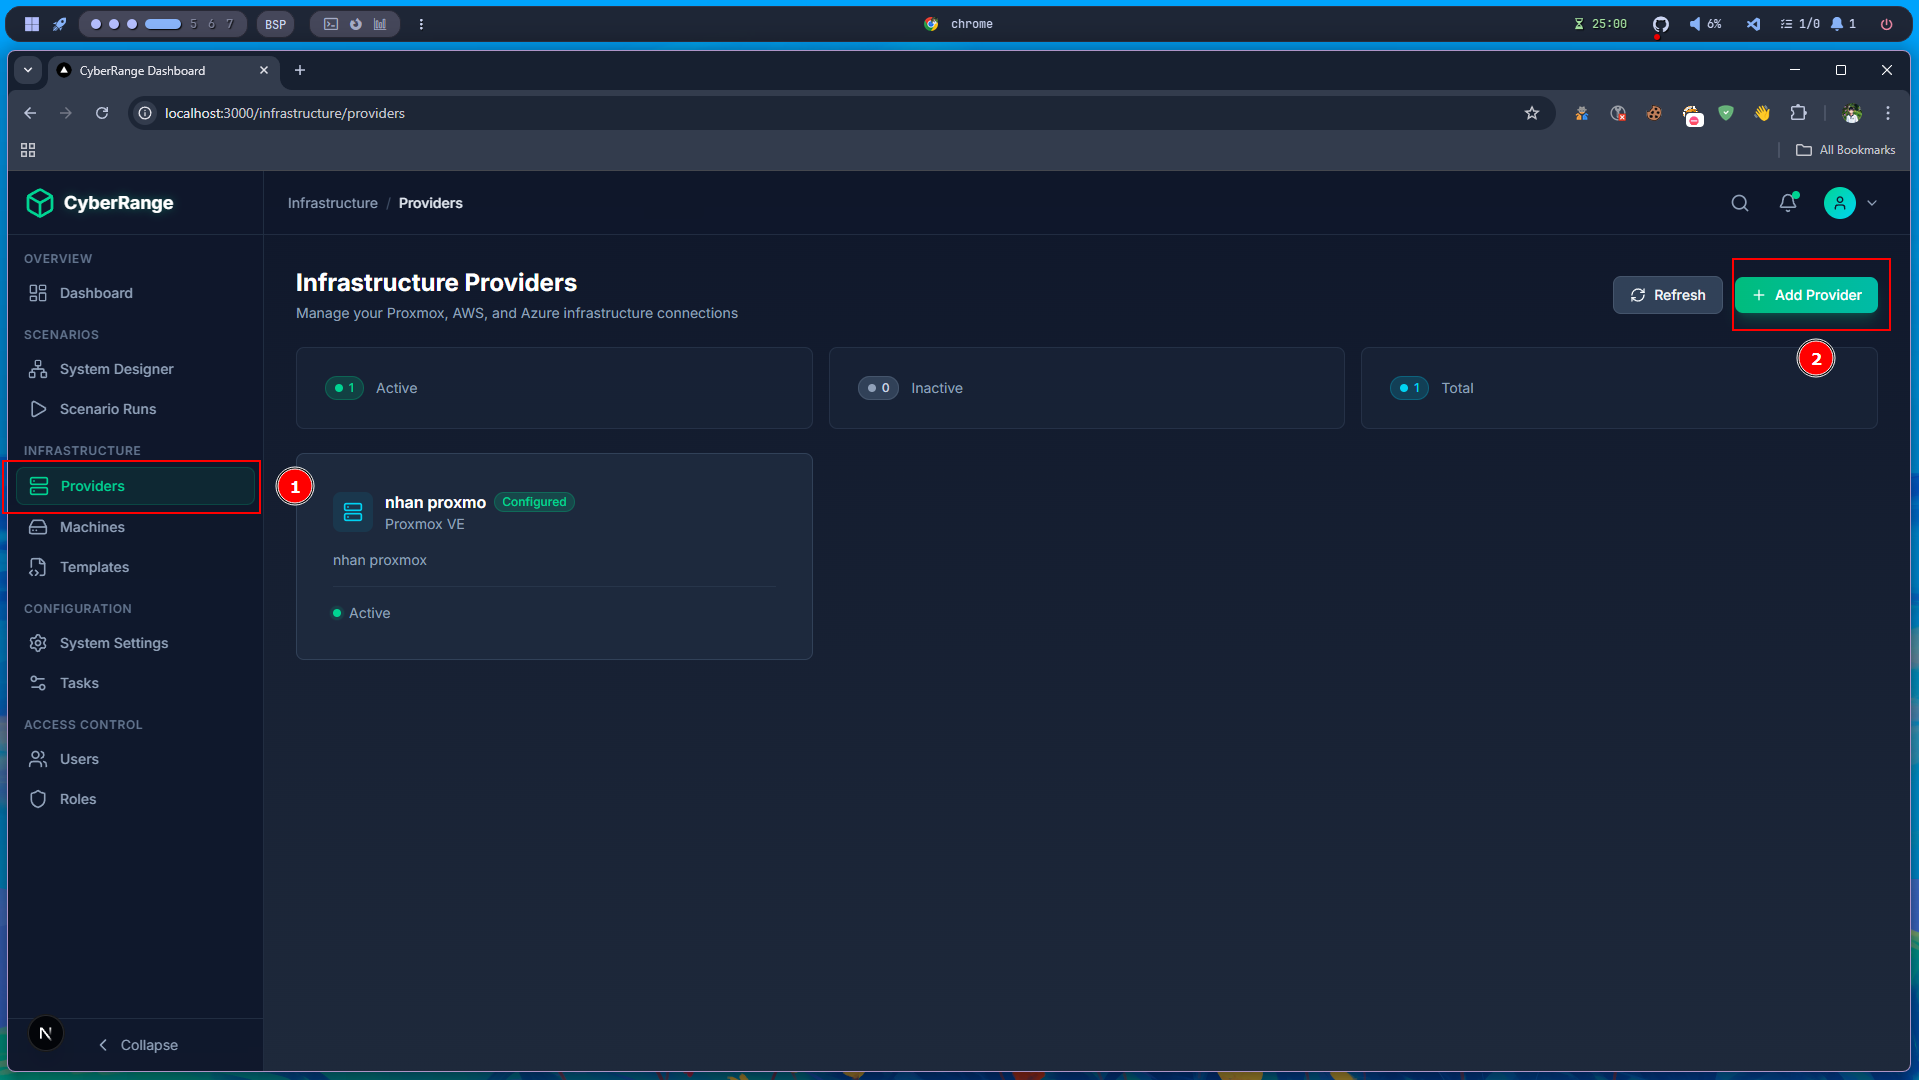
\includegraphics[width=0.95\textwidth]{images/infra/1.png}
    \caption{Provider list view.}
    \label{fig:infra-provider-list}
\end{figure}

\begin{figure}[H]
    \centering
    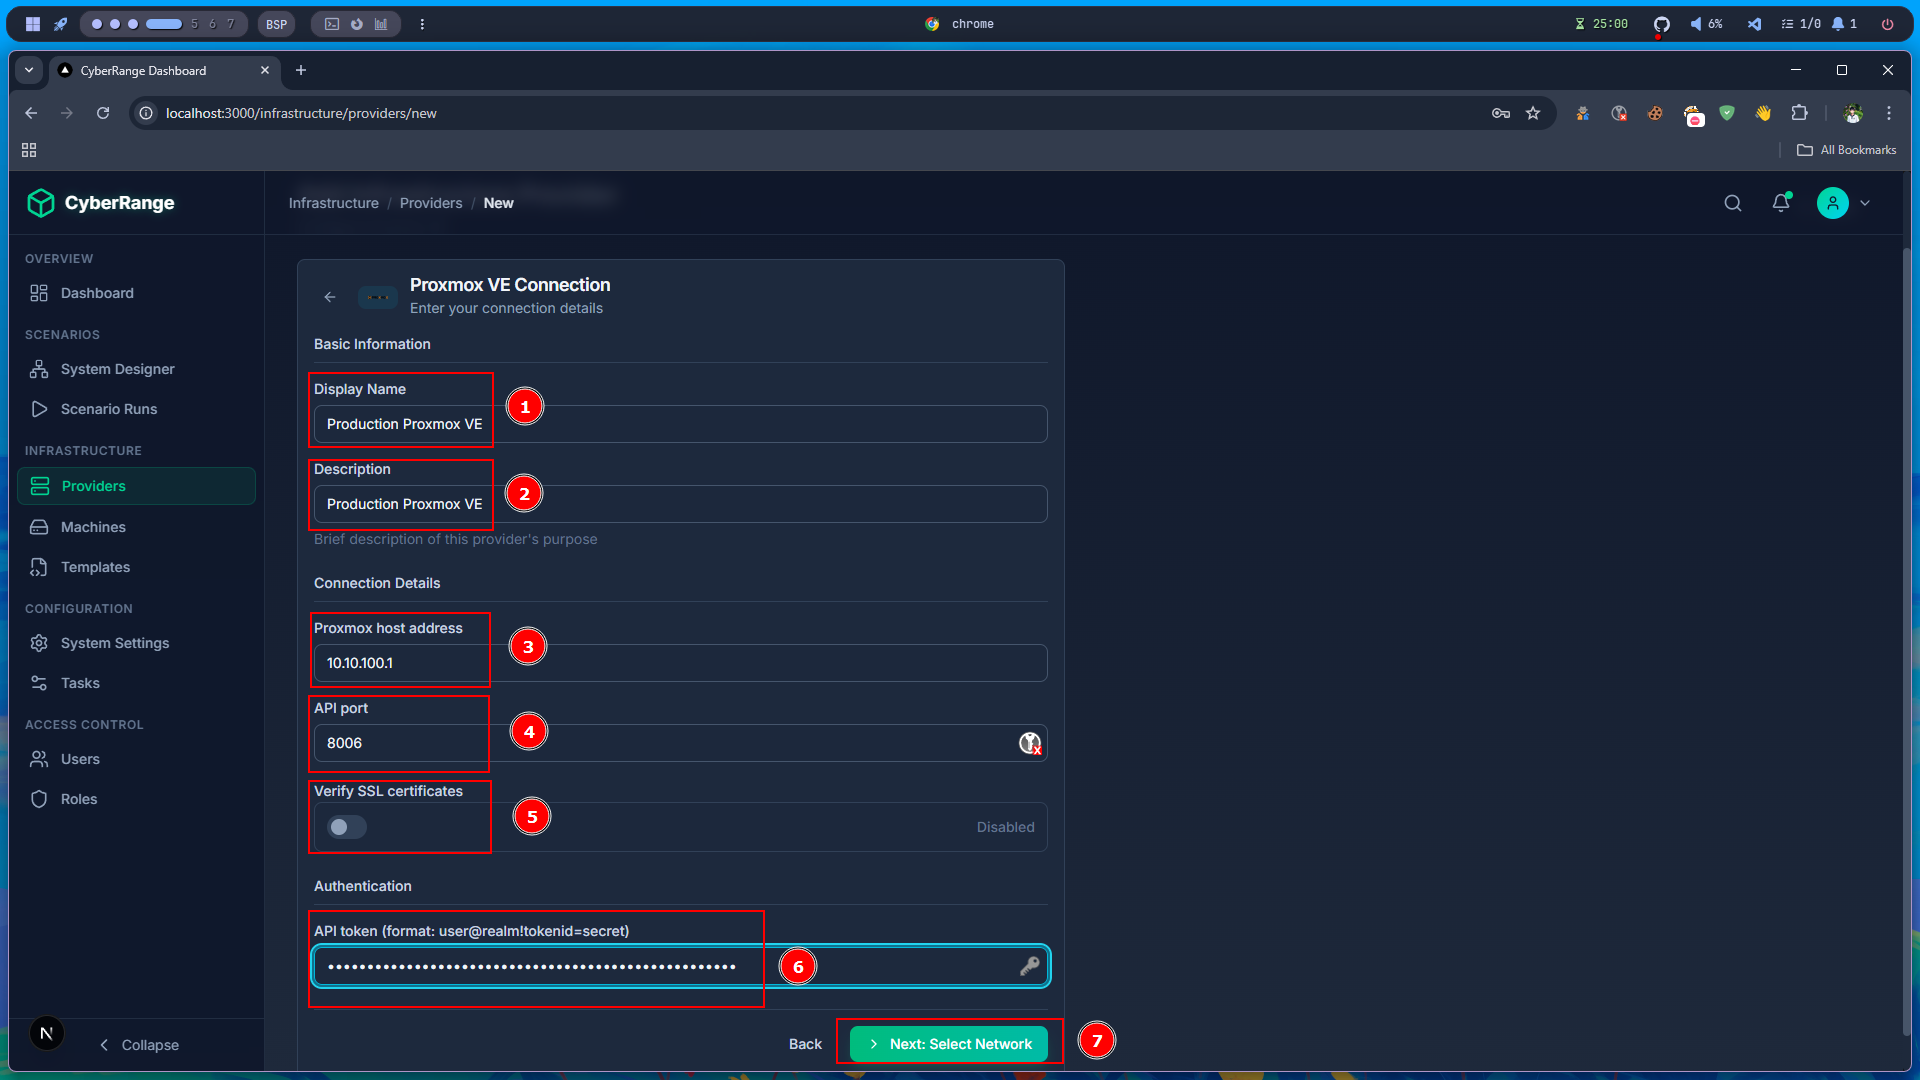
\includegraphics[width=0.95\textwidth]{images/infra/3.png}
    \caption{Proxmox connection form.}
    \label{fig:infra-provider-connection-form}
\end{figure}

\begin{figure}[H]
    \centering
    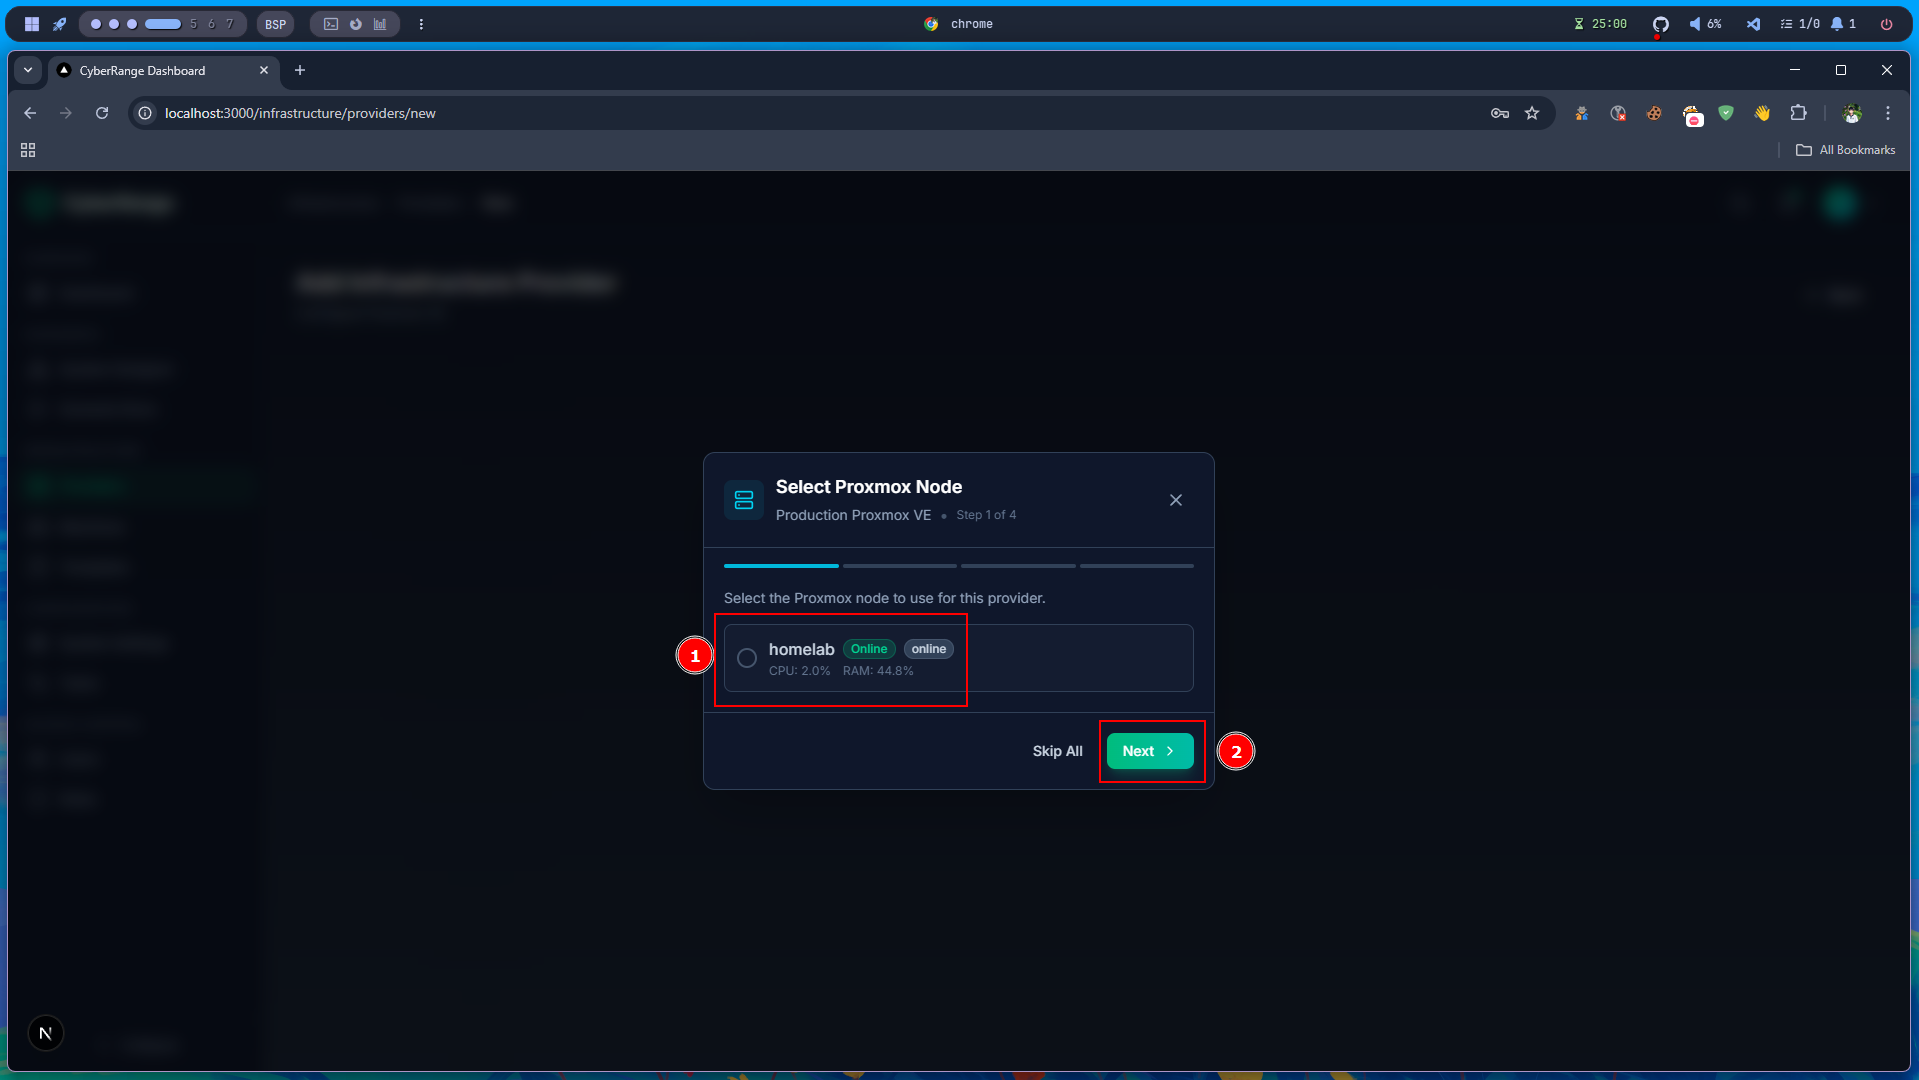
\includegraphics[width=0.95\textwidth]{images/infra/4.png}
    \caption{Proxmox node selection.}
    \label{fig:infra-provider-node-step}
\end{figure}

\begin{figure}[H]
    \centering
    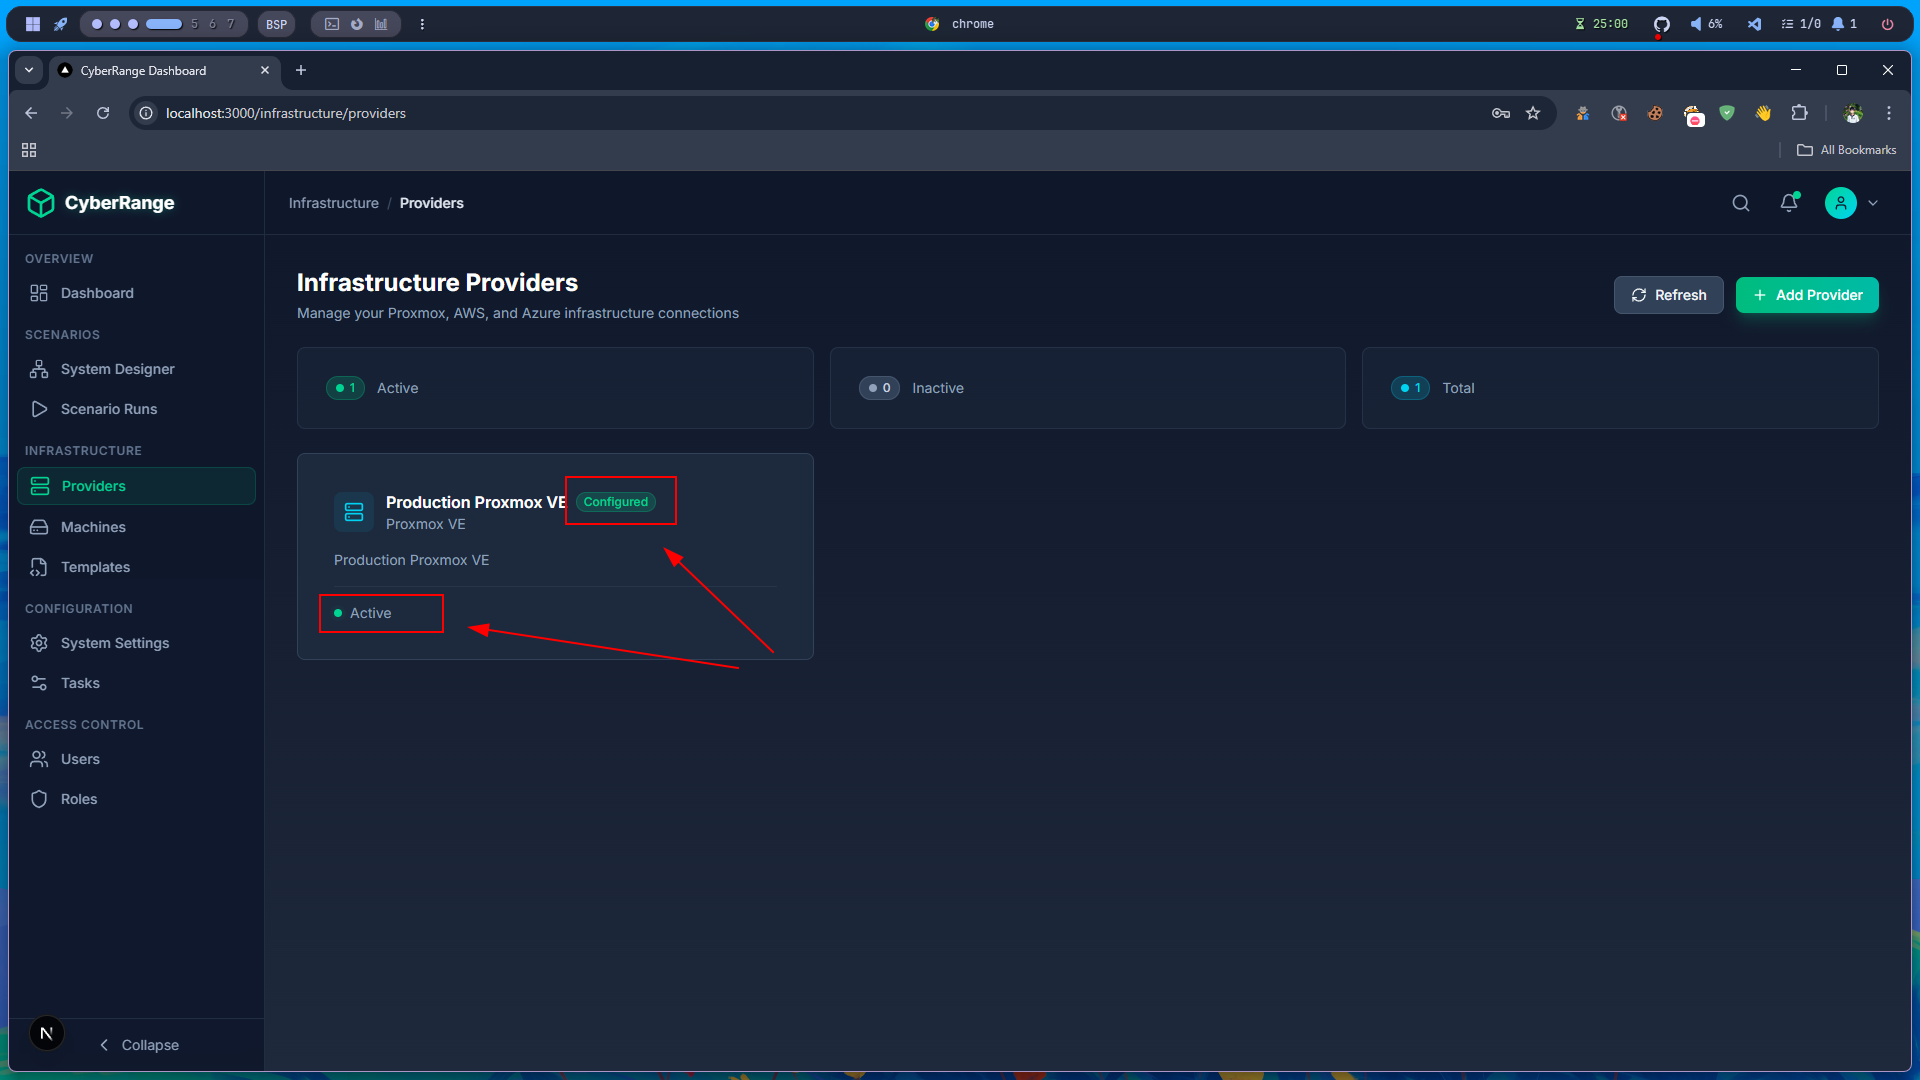
\includegraphics[width=0.95\textwidth]{images/infra/10.png}
    \caption{Configured provider state.}
    \label{fig:infra-provider-configured}
\end{figure}

\subsection{Phase 2: Template and Resource Preparation}
The objective of this phase was to prepare reusable deployment artifacts and resource definitions that support repeatable scenario instantiation. Core functions included template registration, metadata organization, resource mapping, machine synchronization, and readiness validation for deployment reuse.

This phase contributes implementation stability by reducing manual provisioning variance. Reusable templates ensure that scenario runs are created from consistent baselines, which improves reproducibility and simplifies troubleshooting. In the implemented platform, this phase is supported by both the infrastructure-side Proxmox inventory and the dashboard-side template and machine management views.

The operational workflow for template and resource preparation is as follows:

\begin{enumerate}
    \item Verify that the Proxmox node already contains the required base machines, network segments, and storage resources for cyber-range provisioning.
    \item Open \texttt{Infrastructure $\rightarrow$ Templates} to register or refresh reusable Packer templates from source repositories.
    \item Validate template status so only ready-to-use images are exposed to later scenario design and deployment workflows.
    \item Open \texttt{Infrastructure $\rightarrow$ Machines} to synchronize provisioned VMs/LXC resources and confirm runtime status, node placement, and resource allocation.
    \item Reuse these prepared templates and synchronized machines as stable infrastructure inputs for scenario instantiation.
\end{enumerate}

\begin{figure}[H]
    \centering
    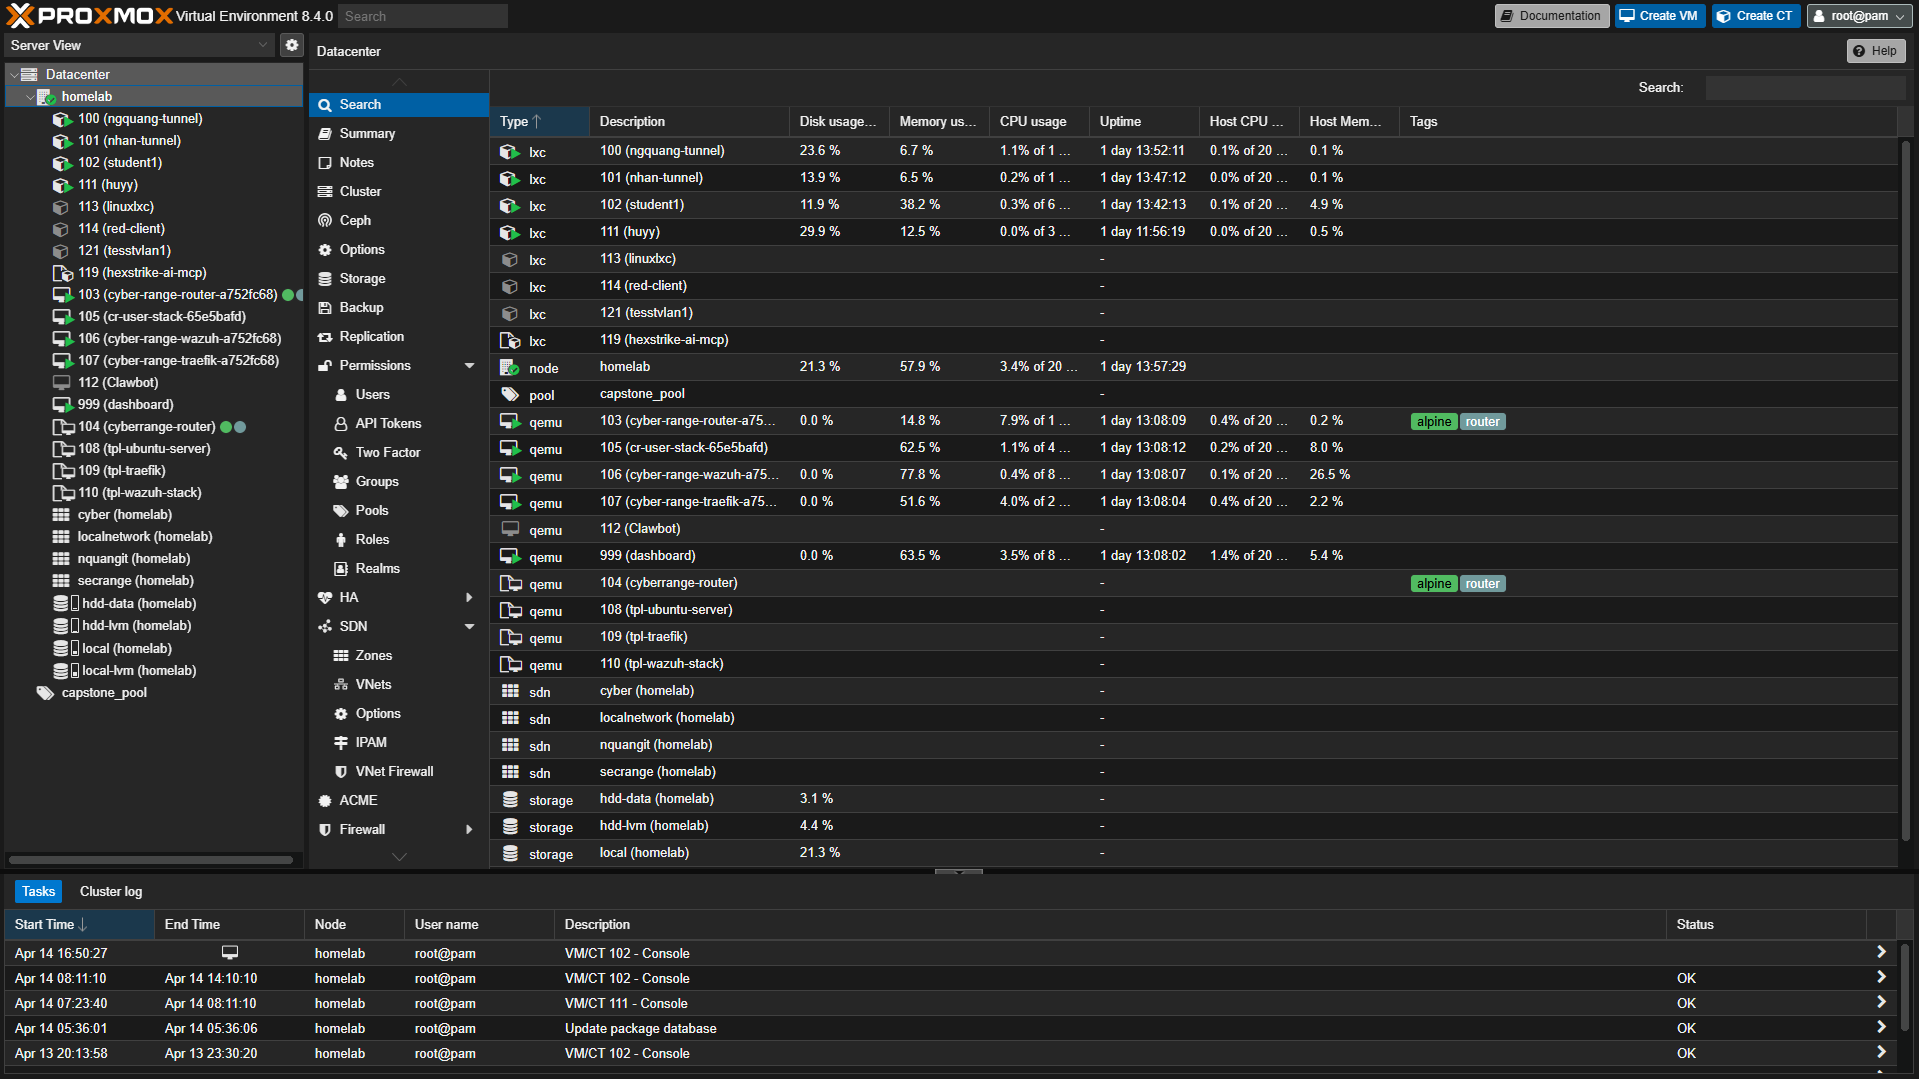
\includegraphics[width=0.95\textwidth]{images/wweb/promox.png}
    \caption{Proxmox inventory view.}
    \label{fig:phase2-proxmox-inventory}
\end{figure}

\begin{figure}[H]
    \centering
    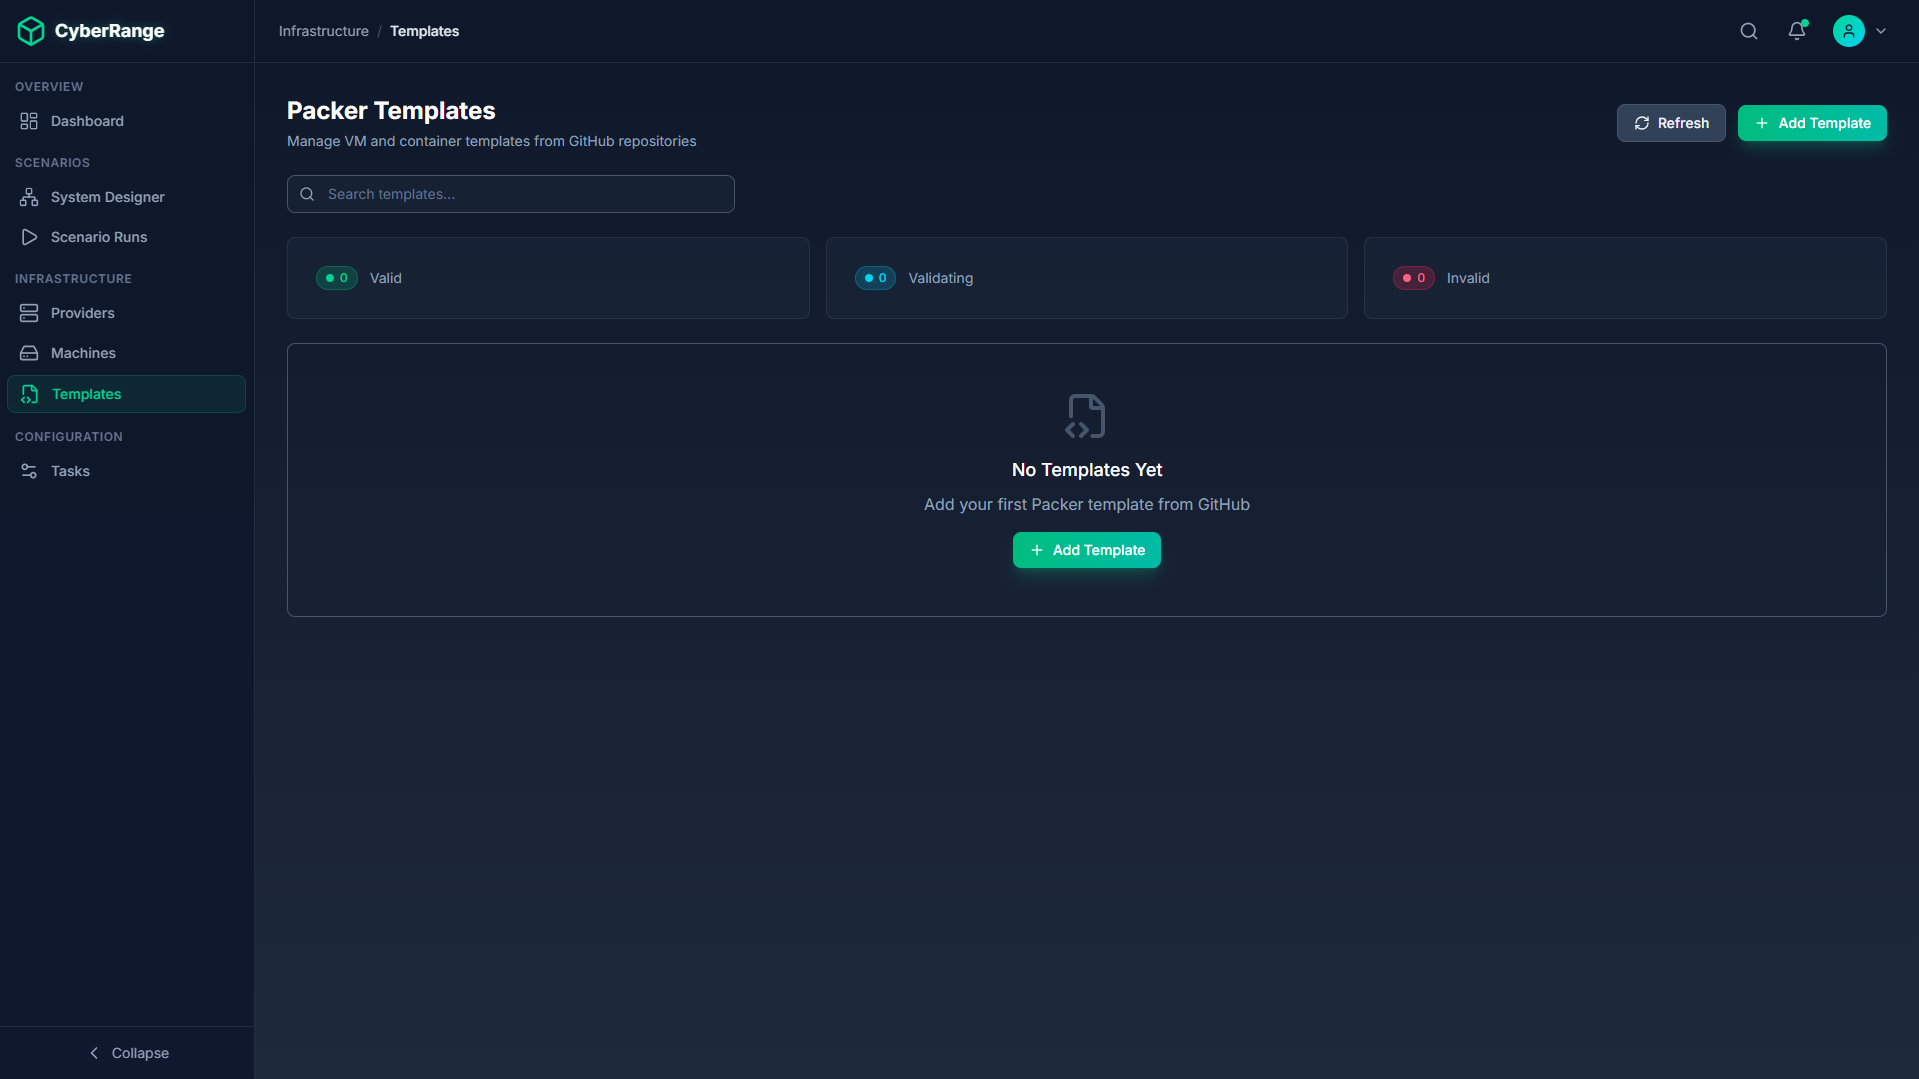
\includegraphics[width=0.95\textwidth]{images/wweb/template.png}
    \caption{Packer template management.}
    \label{fig:phase2-template-management}
\end{figure}

\begin{figure}[H]
    \centering
    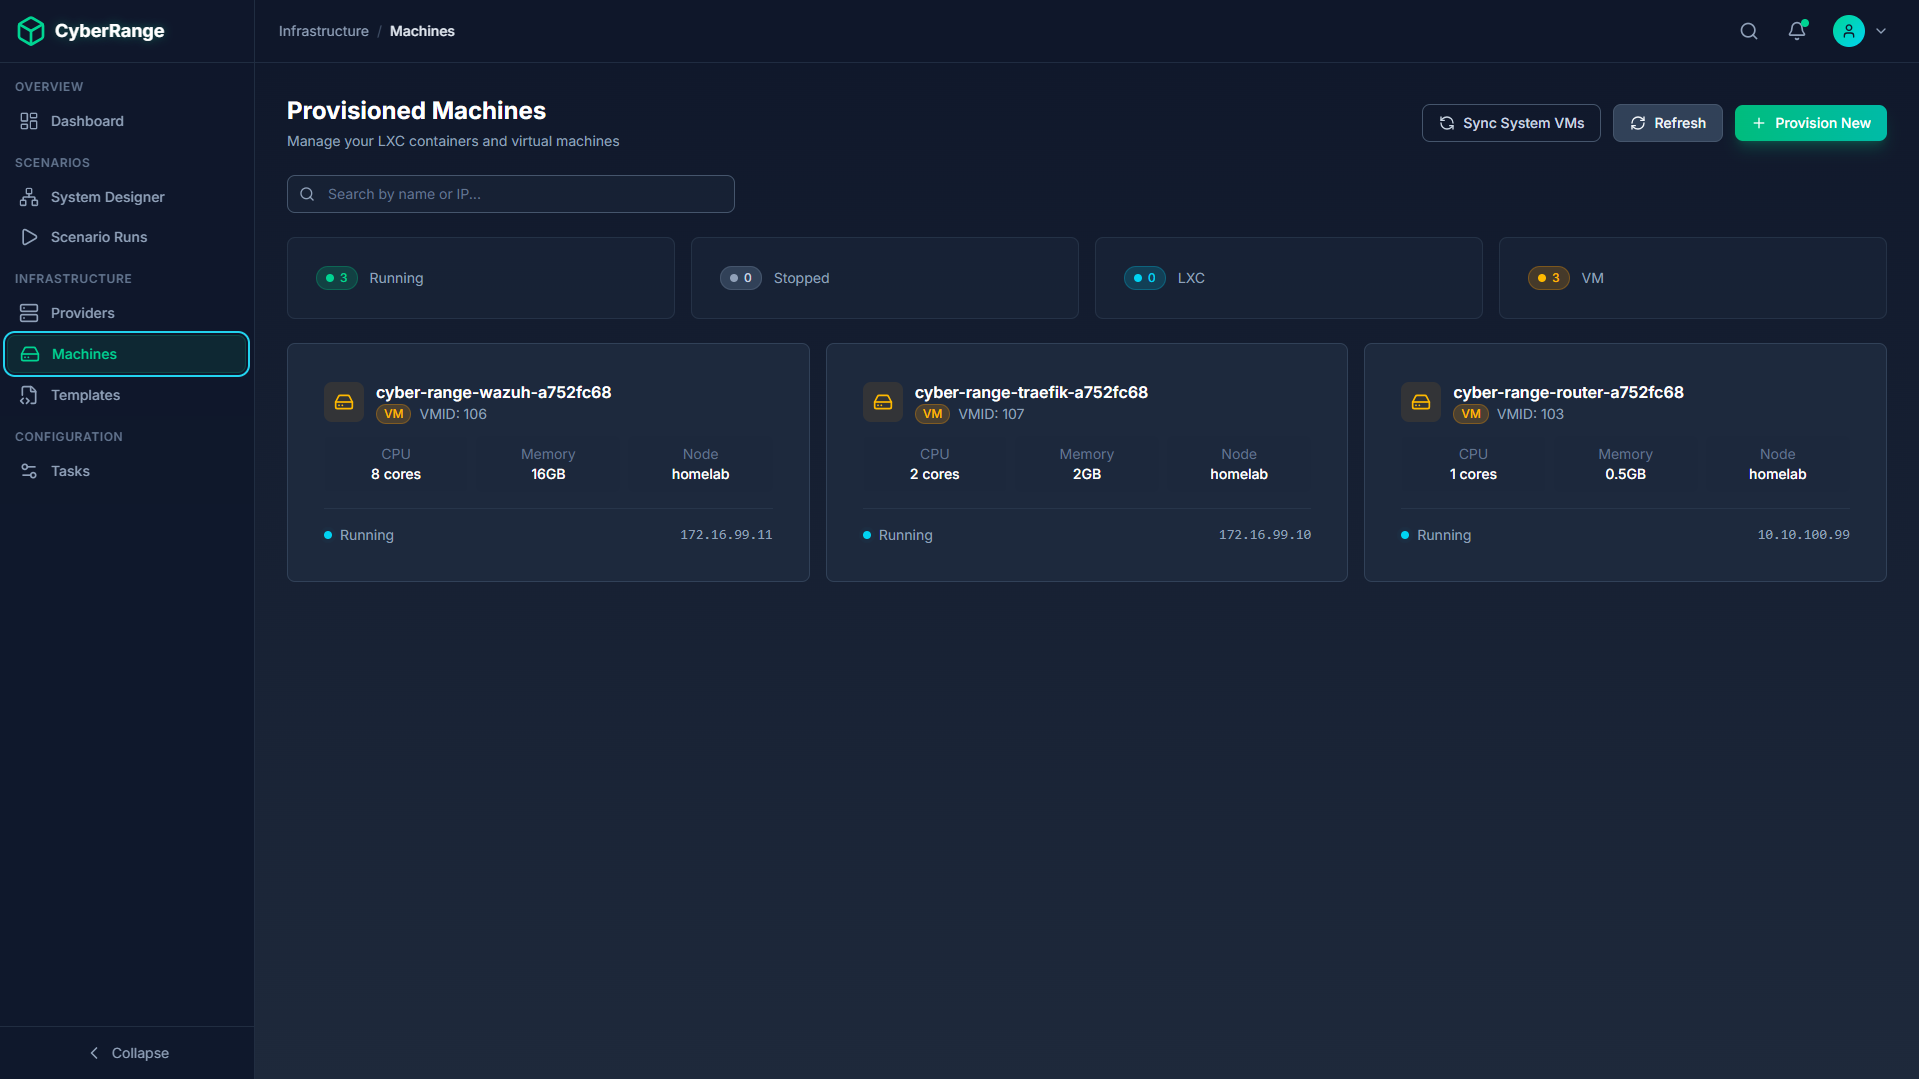
\includegraphics[width=0.95\textwidth]{images/wweb/machine.png}
    \caption{Provisioned machine view.}
    \label{fig:phase2-machine-management}
\end{figure}

\subsection{Phase 3: Scenario Definition and Management}
The objective of this phase was to formalize executable training logic through scenario entities. Core functions included scenario creation, update and version control, linkage to provider/template assets, and lifecycle state management.

This phase bridges static infrastructure preparation and dynamic execution. By encapsulating deployment logic into scenario definitions, the platform enables controlled and repeatable training workflows through the dashboard.

The scenario authoring workflow is captured in \texttt{images/scenarios}. The validated sequence used in implementation is:

\begin{enumerate}
    \item Open \texttt{Scenarios $\rightarrow$ System Designer}, then select \texttt{New Scenario}.
    \item Enter scenario name and description, then bind the scenario to a configured infrastructure provider.
    \item Use the visual editor to drag and place runtime components into the user stack topology.
    \item Configure node-level parameters on the right panel (for example API key bindings for Blue Team/Red Team agents).
    \item For custom application containers, select Docker Compose mode, provide repository and branch, verify compose metadata, and map exposed ports.
    \item Save scenario changes before triggering deployment.
\end{enumerate}

In the implemented system, the platform provides three ready-made scenarios so that instructors or learners can launch training environments without designing the topology from scratch. The first is a \textit{Red Team Single} scenario, in which the learner is provided with a dedicated WAF interface, a Red Team attack workspace, and a vulnerable target web application. This scenario is designed for offensive practice and includes AI-assisted support to help interpret attack attempts and request behavior.

The second is a \textit{Blue Team Single} scenario, in which the learner is provided with a WAF layer together with a Blue Team analysis interface for log inspection, alert review, and AI-assisted interpretation. In the current implementation, this defensive workspace is delivered through the BlueAgent WAF Console presented later in this chapter. This scenario emphasizes defensive analysis, allowing trainees to focus on monitoring evidence and understanding how suspicious requests are detected and explained.

The third is a \textit{Dual} scenario, which combines both operational perspectives into one linked environment. In this mode, the Red Team attacks the target web application while the resulting traffic and security events are forwarded to the Blue Team workspace for investigation. This linkage creates a more realistic end-to-end cyber range exercise in which offensive actions produce defensive telemetry that can be reviewed in near real time.

To support these scenarios, the project includes a vulnerable SQL-focused target application used as an attack surface during training. This target application is paired with the Red Team workspace in offensive exercises and becomes the common event source for the linked dual scenario.

\begin{figure}[H]
    \centering
    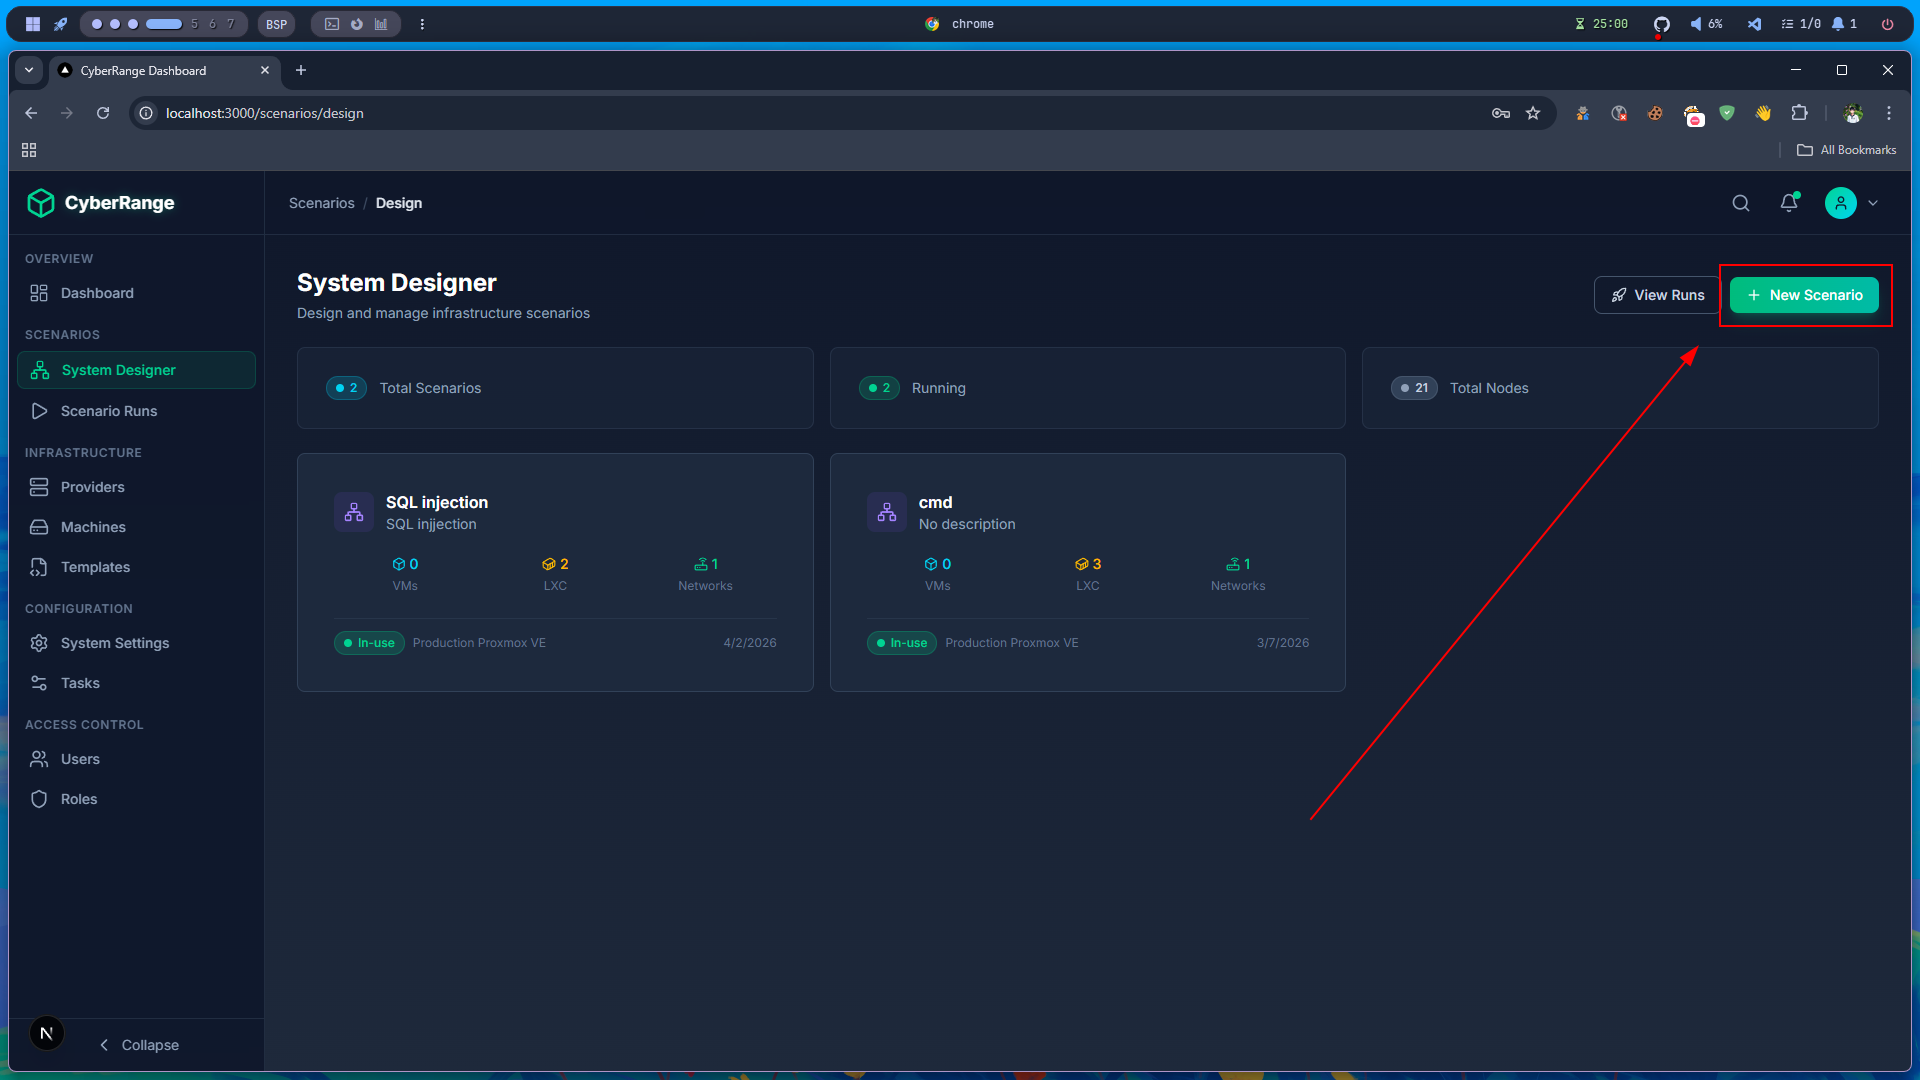
\includegraphics[width=0.95\textwidth]{images/scenarios/1.png}
    \caption{System Designer overview.}
    \label{fig:scenario-designer-entry}
\end{figure}

\begin{figure}[H]
    \centering
    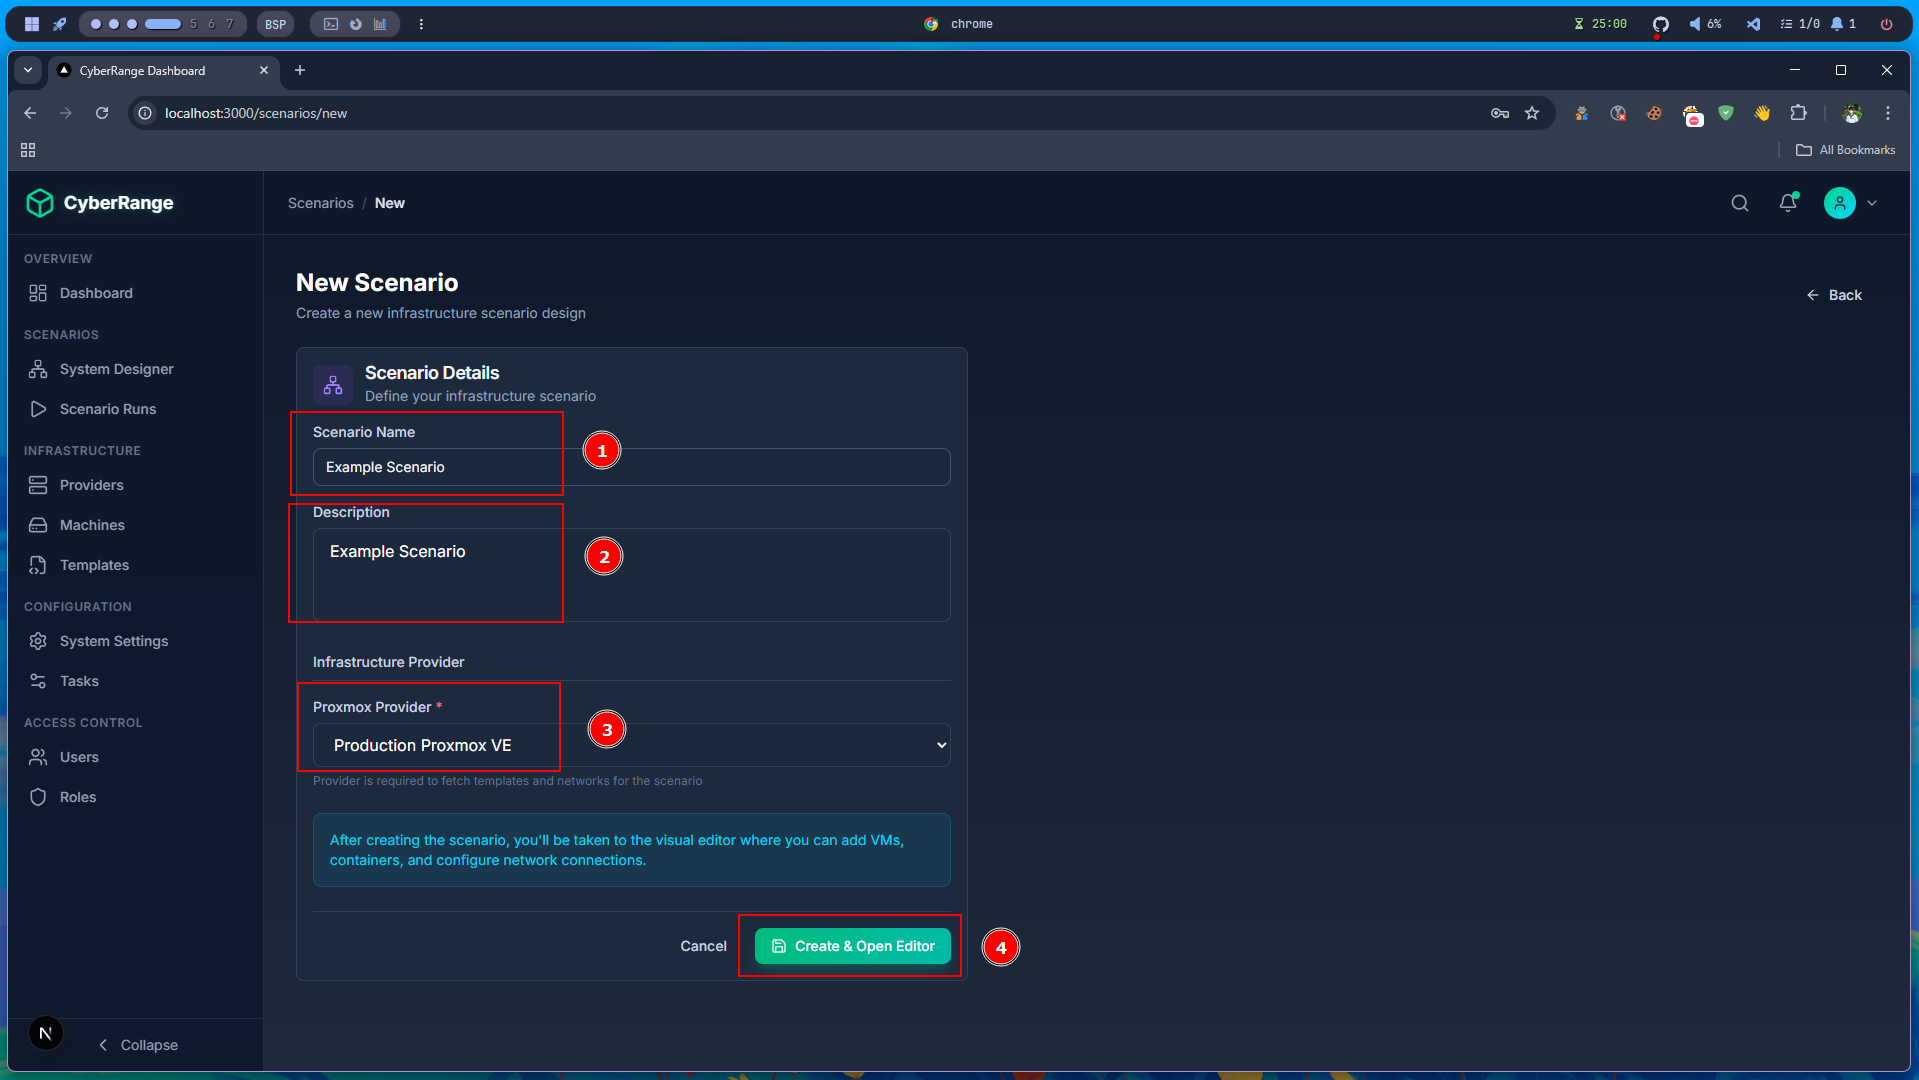
\includegraphics[width=0.95\textwidth]{images/scenarios/2.png}
    \caption{Scenario creation form.}
    \label{fig:scenario-create-form}
\end{figure}

\begin{figure}[H]
    \centering
    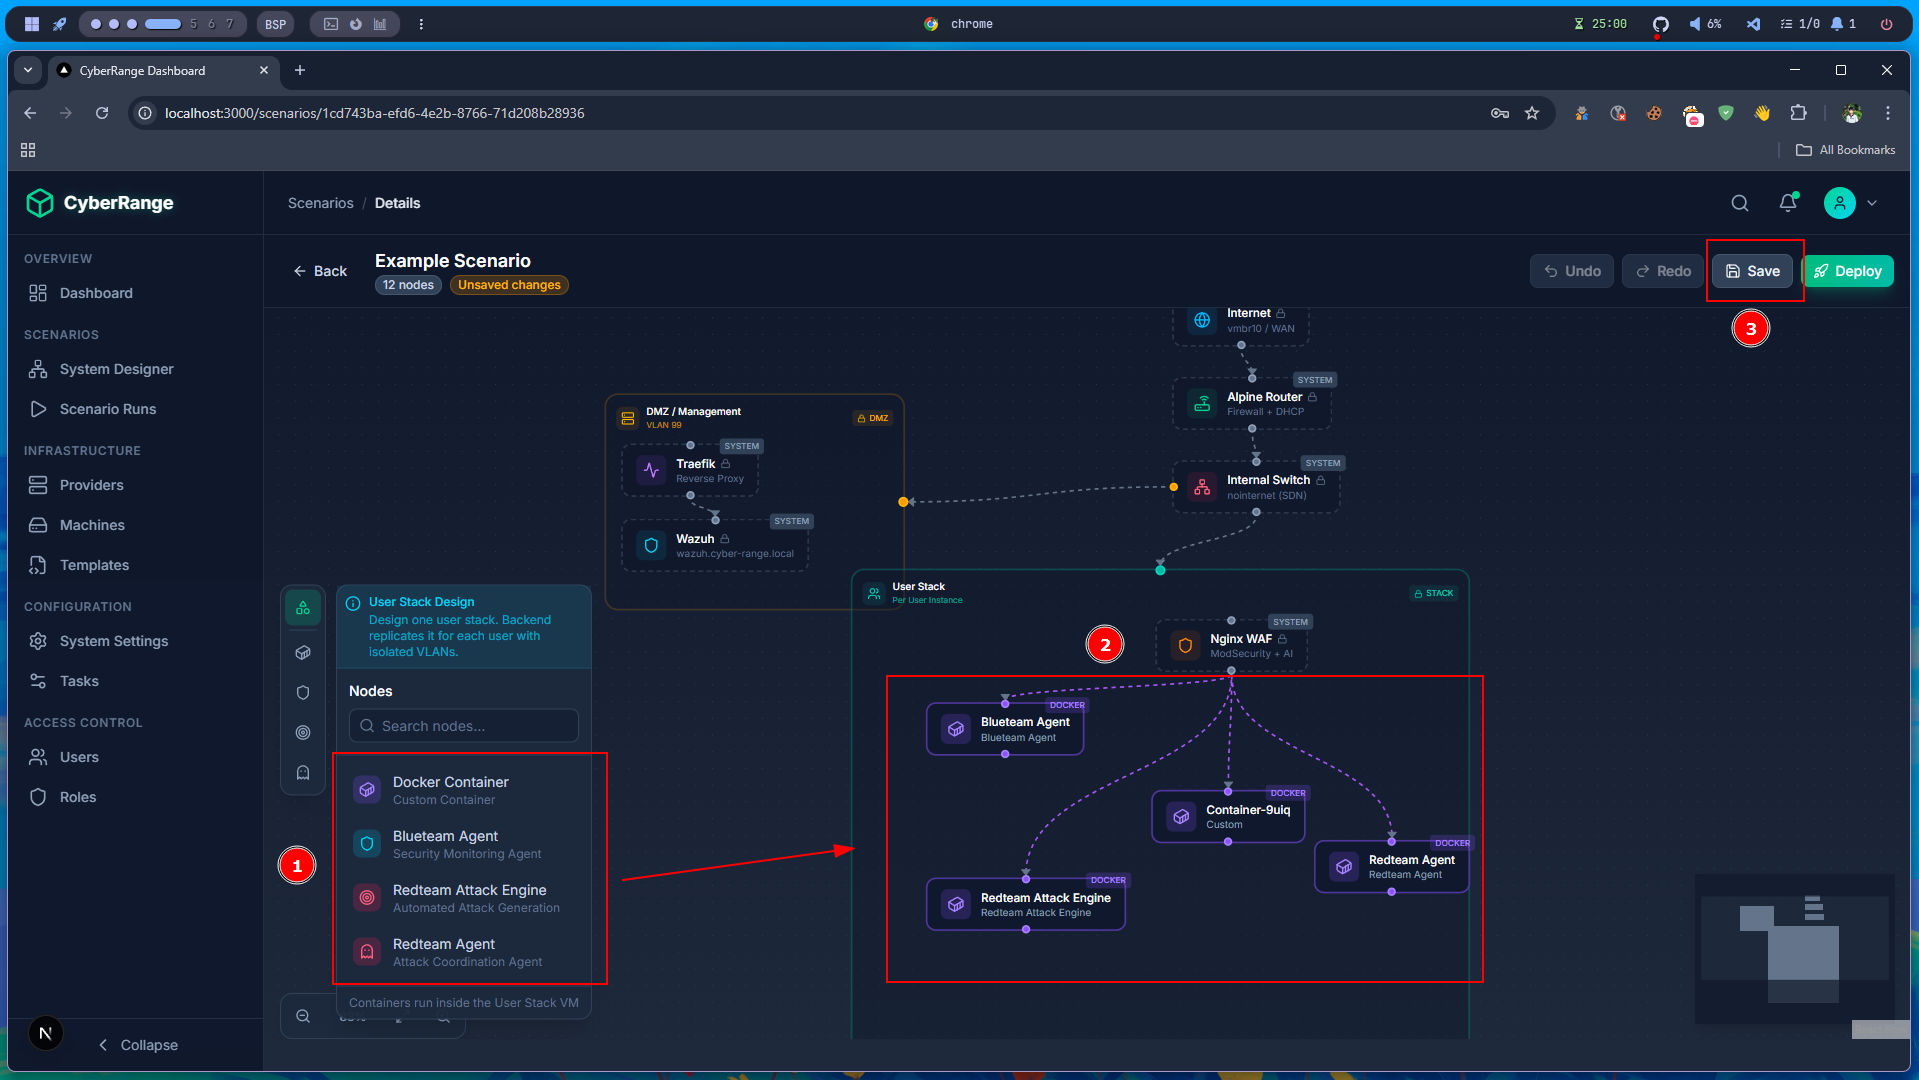
\includegraphics[width=0.95\textwidth]{images/scenarios/3.png}
    \caption{Scenario topology editor.}
    \label{fig:scenario-visual-editor}
\end{figure}

\begin{figure}[H]
    \centering
    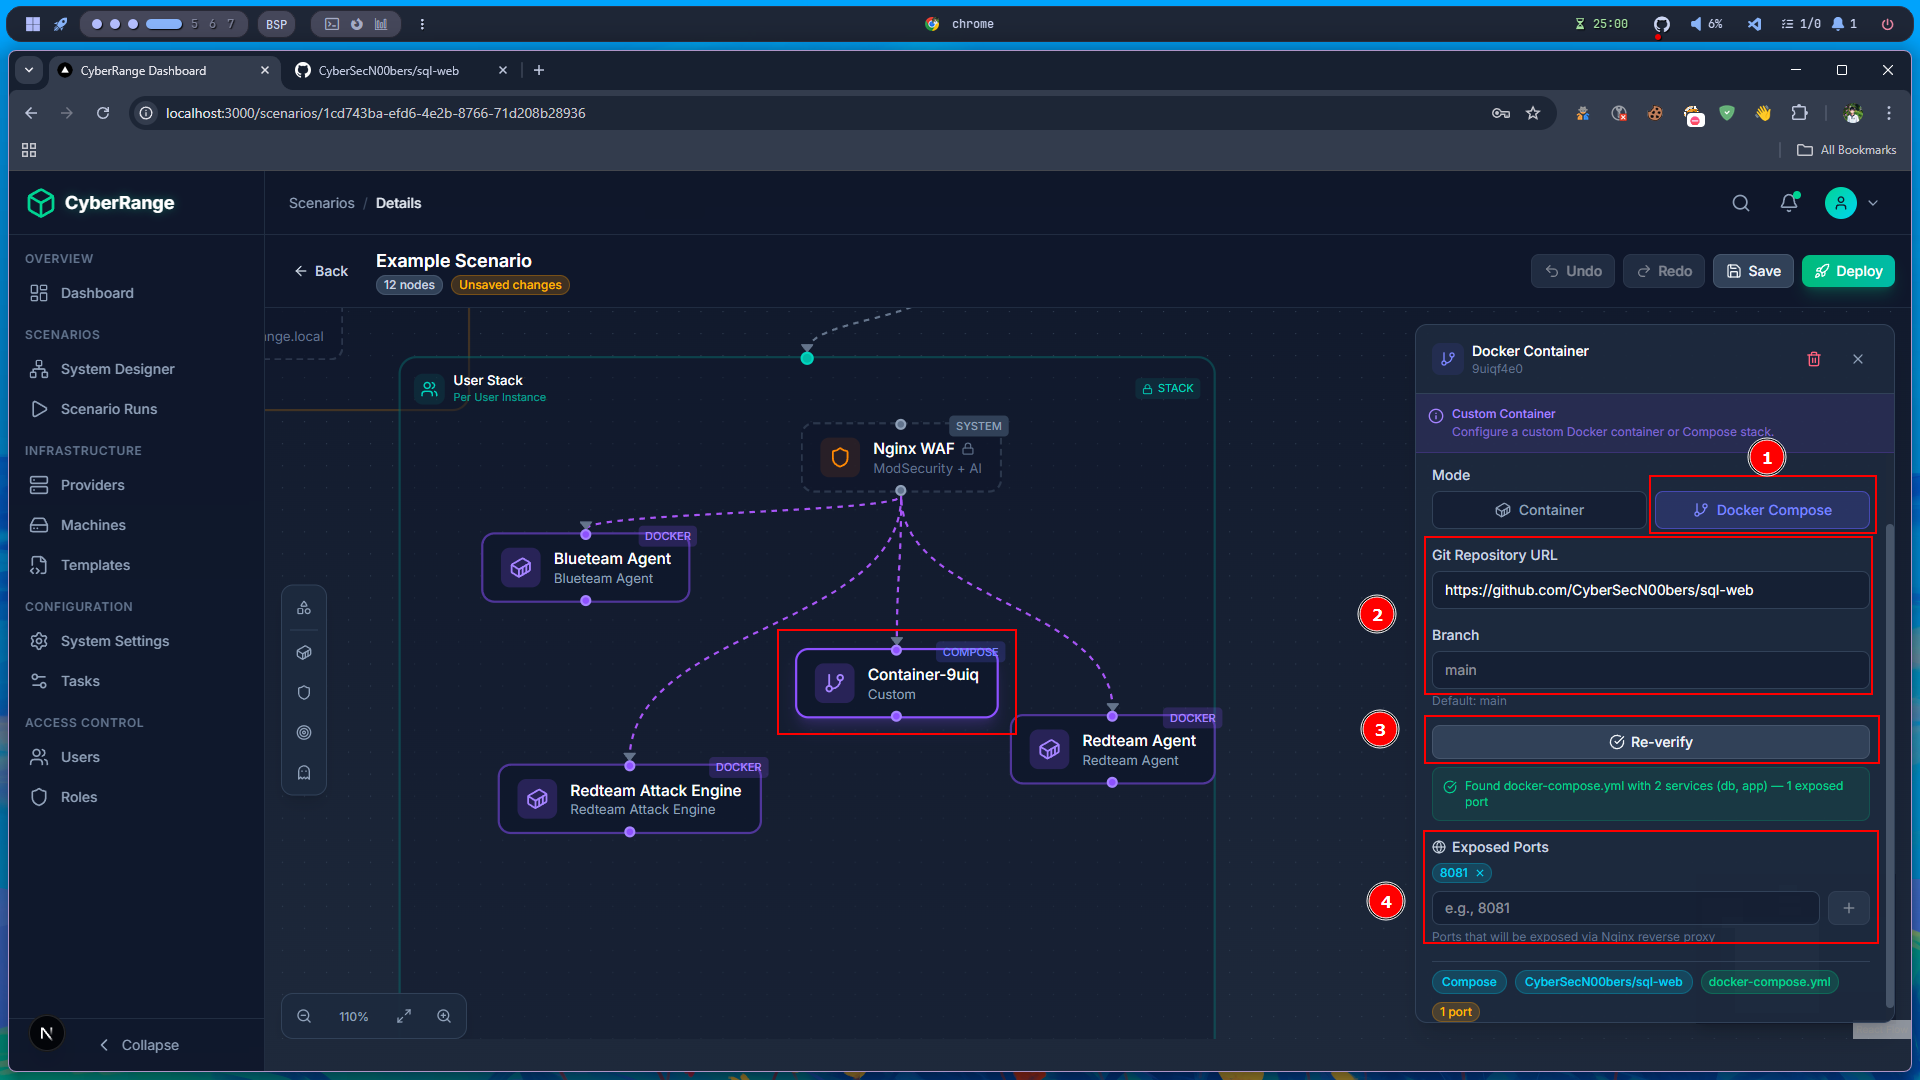
\includegraphics[width=0.95\textwidth]{images/scenarios/5.png}
    \caption{Custom container configuration.}
    \label{fig:scenario-docker-compose-config}
\end{figure}

\begin{figure}[H]
    \centering
    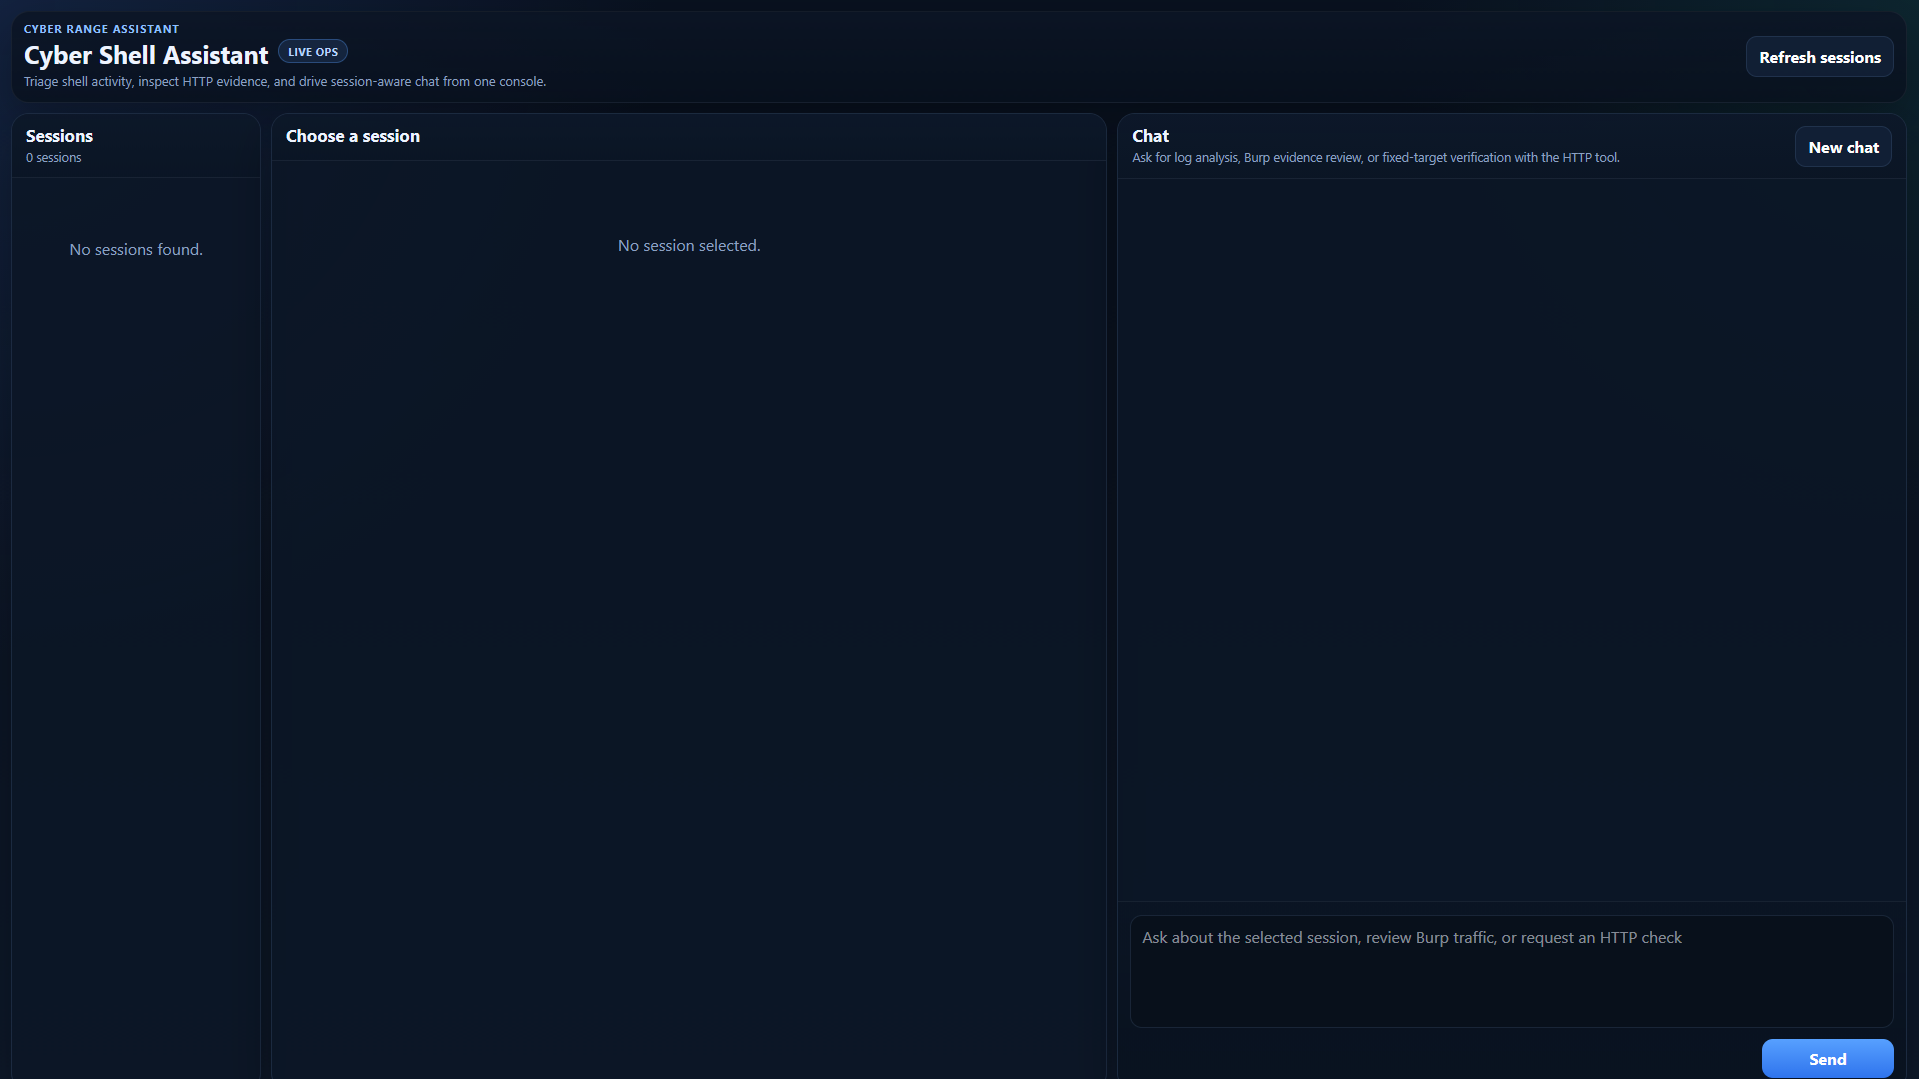
\includegraphics[width=0.95\textwidth]{images/wweb/redtam agent.png}
    \caption{Red Team single-scenario workspace with AI-assisted attack support.}
    \label{fig:scenario-redteam-workspace}
\end{figure}

\begin{figure}[H]
    \centering
    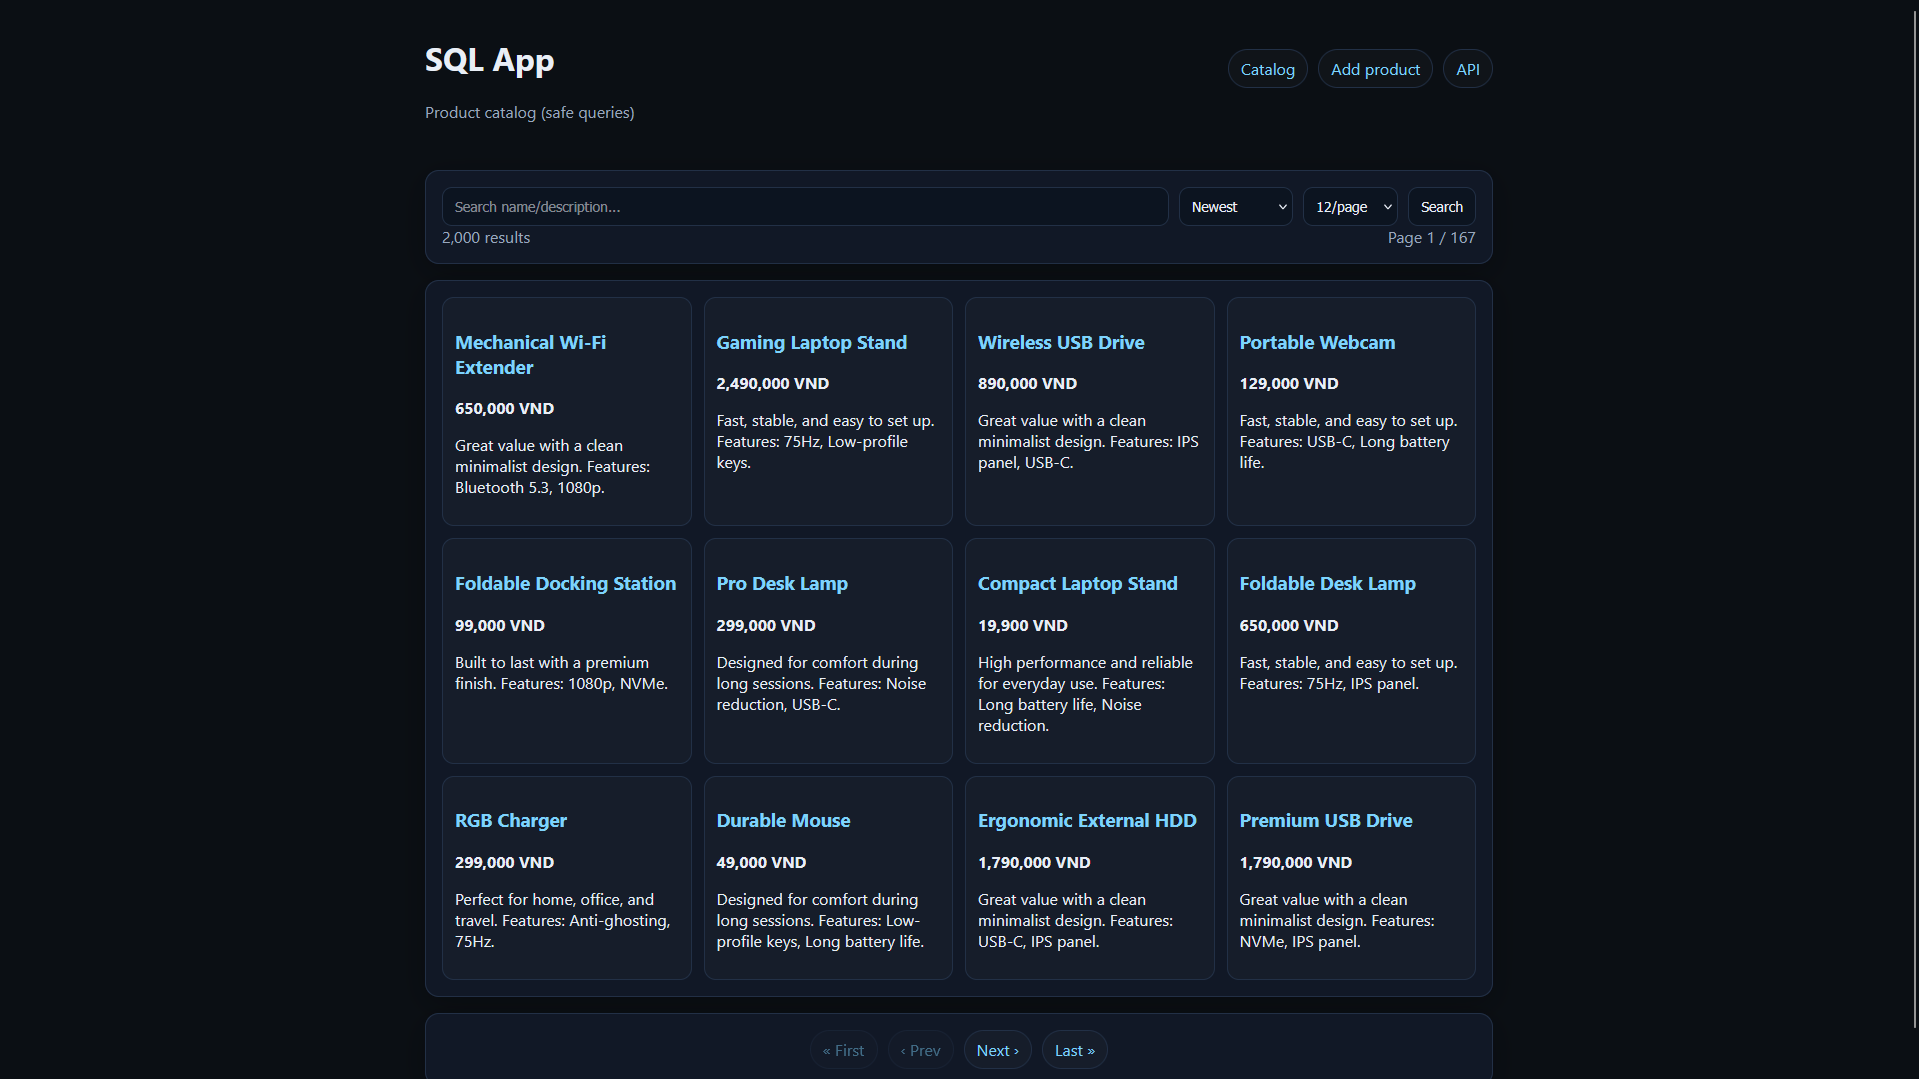
\includegraphics[width=0.95\textwidth]{images/wweb/sqlapp.png}
    \caption{Vulnerable SQL target web application used in predefined scenarios.}
    \label{fig:scenario-sqlapp-target}
\end{figure}

\subsection{Phase 4: Scenario Deployment and Execution}
The objective of this phase was to execute scenario provisioning through asynchronous orchestration. Core functions included deployment triggering, job dispatch, runtime state transitions, and execution feedback propagation to dashboard views.

This phase is operationally central because it transforms configuration artifacts into active training environments. Asynchronous execution is essential here because deployment operations are long-running and cannot block dashboard responsiveness.

The deployment and post-deployment access workflow is documented in \path{images/scenarios/deploy}. The operational steps are:

\begin{enumerate}
    \item From \texttt{System Designer}, open scenario actions and select \texttt{Deploy}.
    \item Move to \texttt{Scenario Runs} to monitor state transitions (pending/running/failed/destroyed).
    \item Open run actions and select \texttt{View Resources} to inspect provisioned assets.
    \item Validate generated domains, runtime applications, and user stack health in the run access page.
    \item Open \texttt{Credentials} to retrieve access details (SSH, service credentials, and generated secrets).
    \item When training is complete, execute \texttt{Destroy} from run actions to release allocated resources.
\end{enumerate}

\begin{figure}[H]
    \centering
    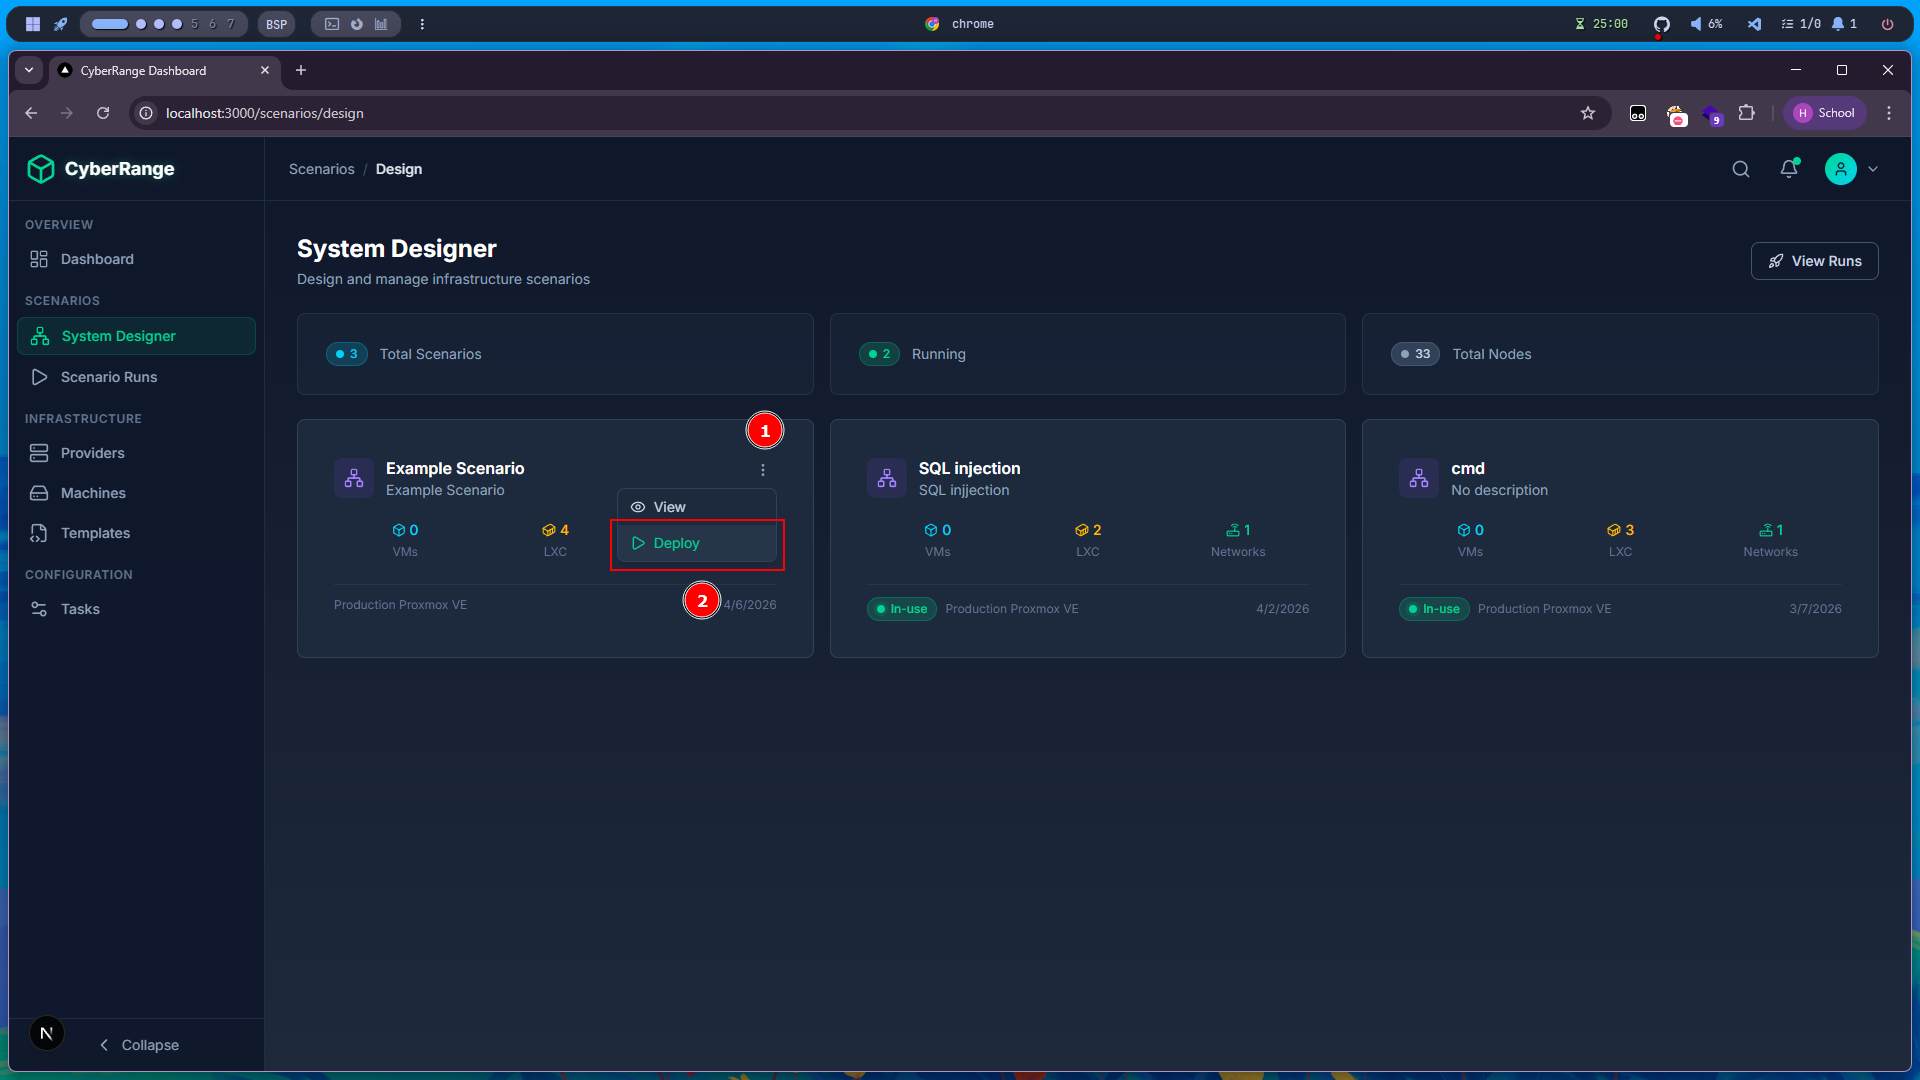
\includegraphics[width=0.95\textwidth]{images/scenarios/deploy/1.png}
    \caption{Scenario deploy action.}
    \label{fig:scenario-deploy-trigger}
\end{figure}

\begin{figure}[H]
    \centering
    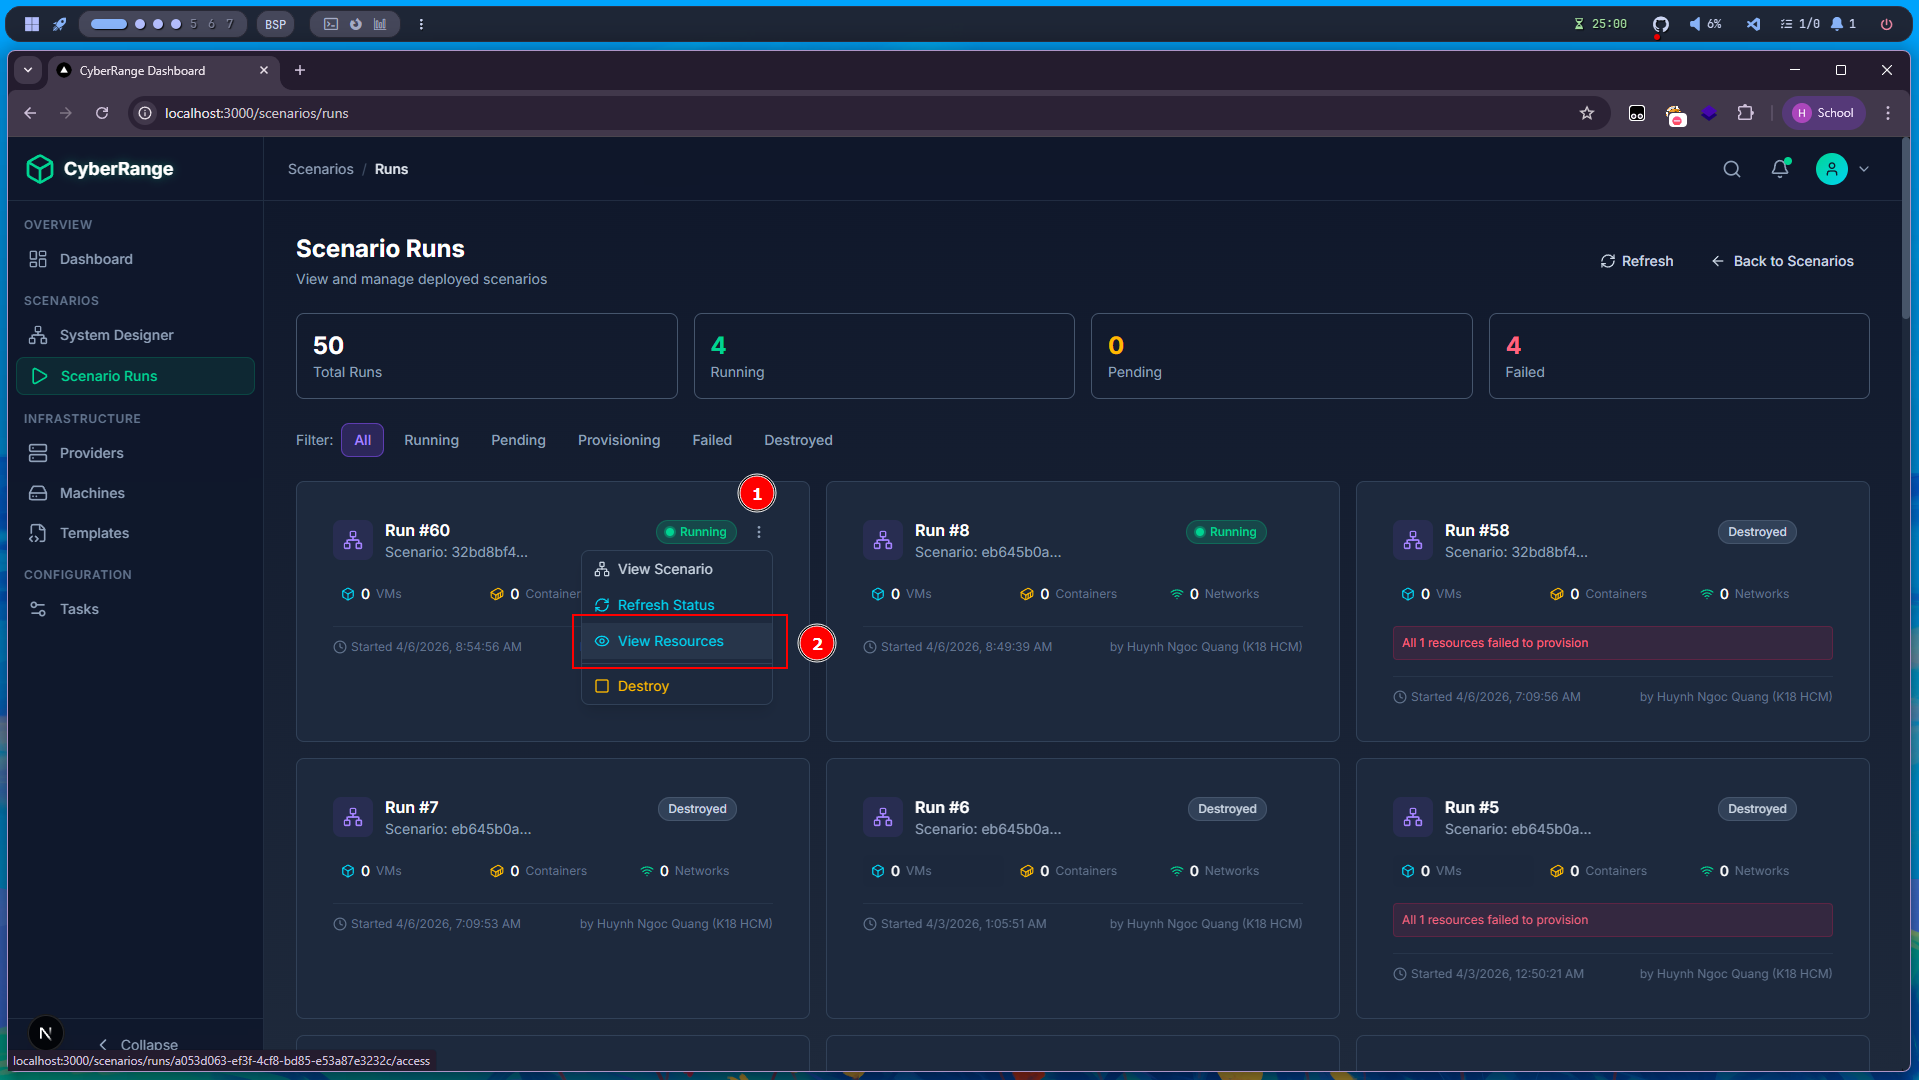
\includegraphics[width=0.95\textwidth]{images/scenarios/deploy/3.png}
    \caption{Run action menu.}
    \label{fig:scenario-run-view-resources}
\end{figure}

\begin{figure}[H]
    \centering
    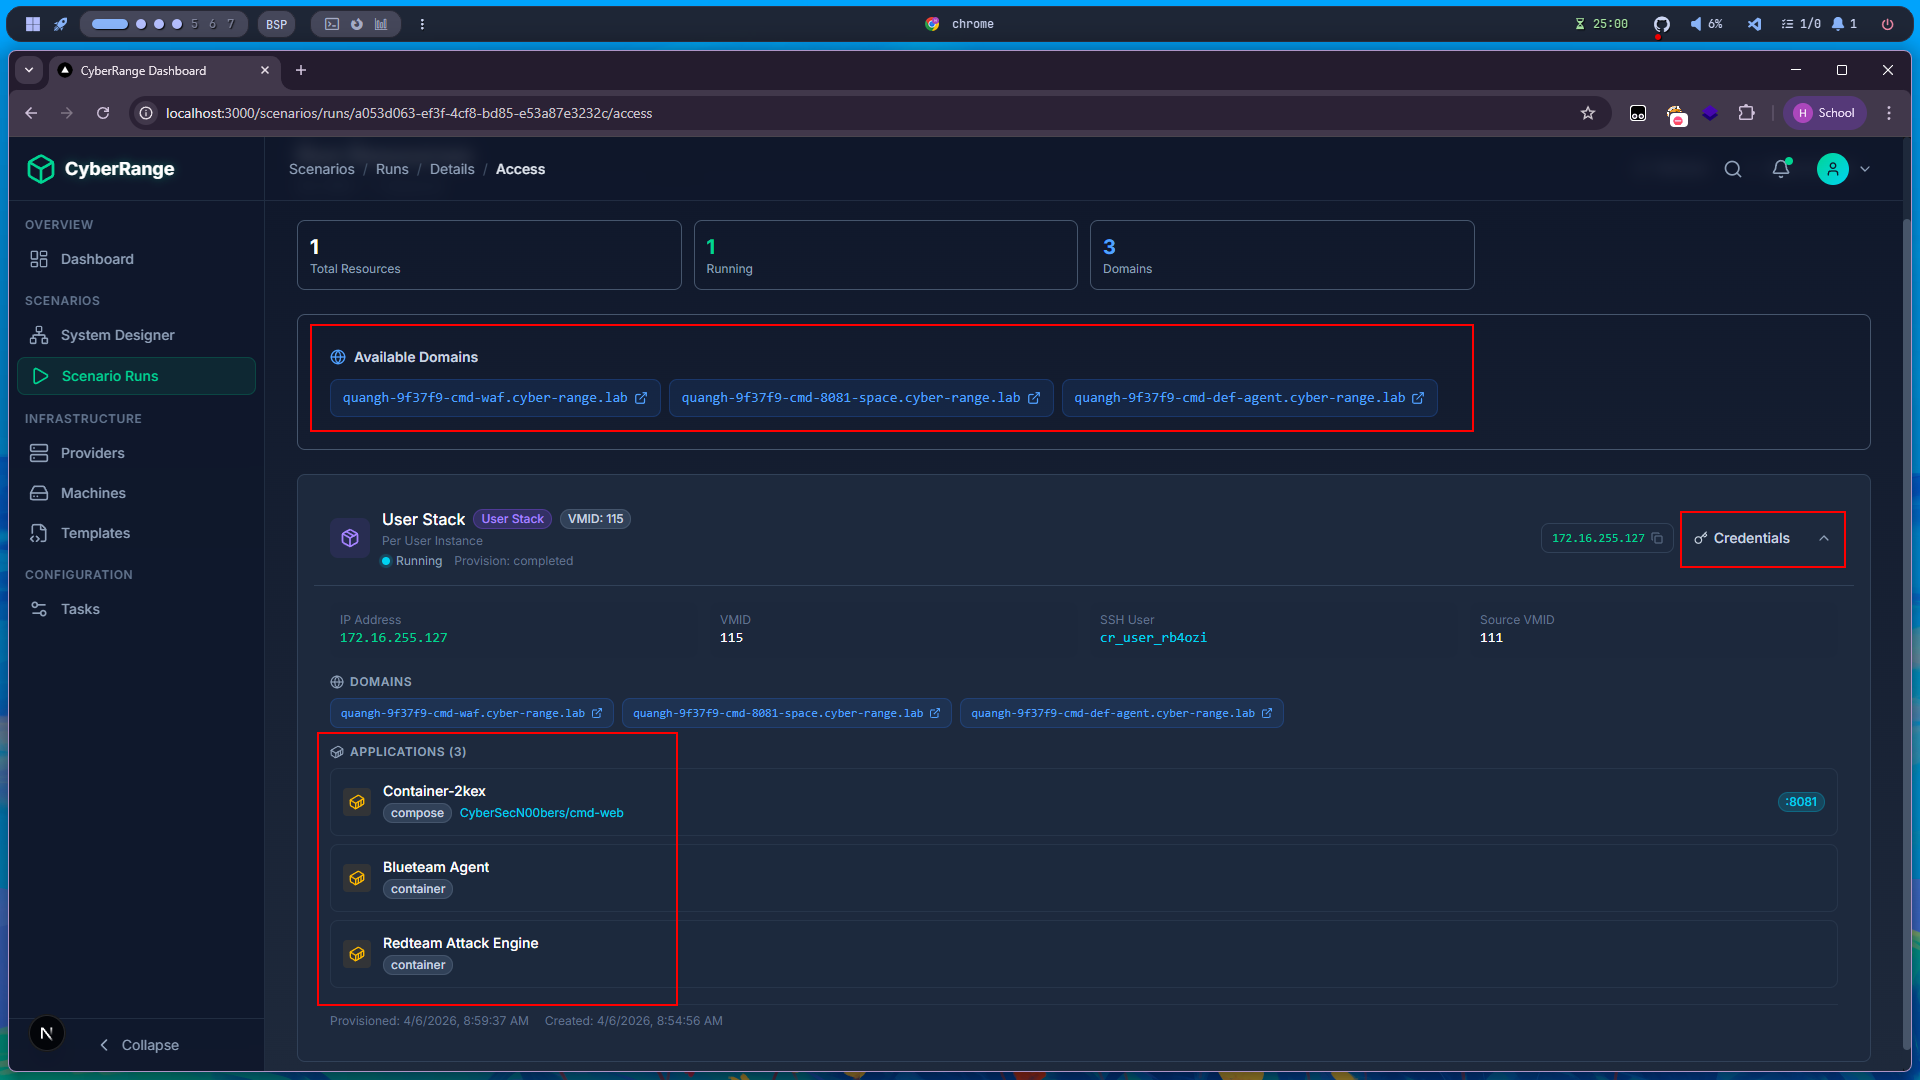
\includegraphics[width=0.95\textwidth]{images/scenarios/deploy/4.png}
    \caption{Run access view.}
    \label{fig:scenario-run-access-view}
\end{figure}

\begin{figure}[H]
    \centering
    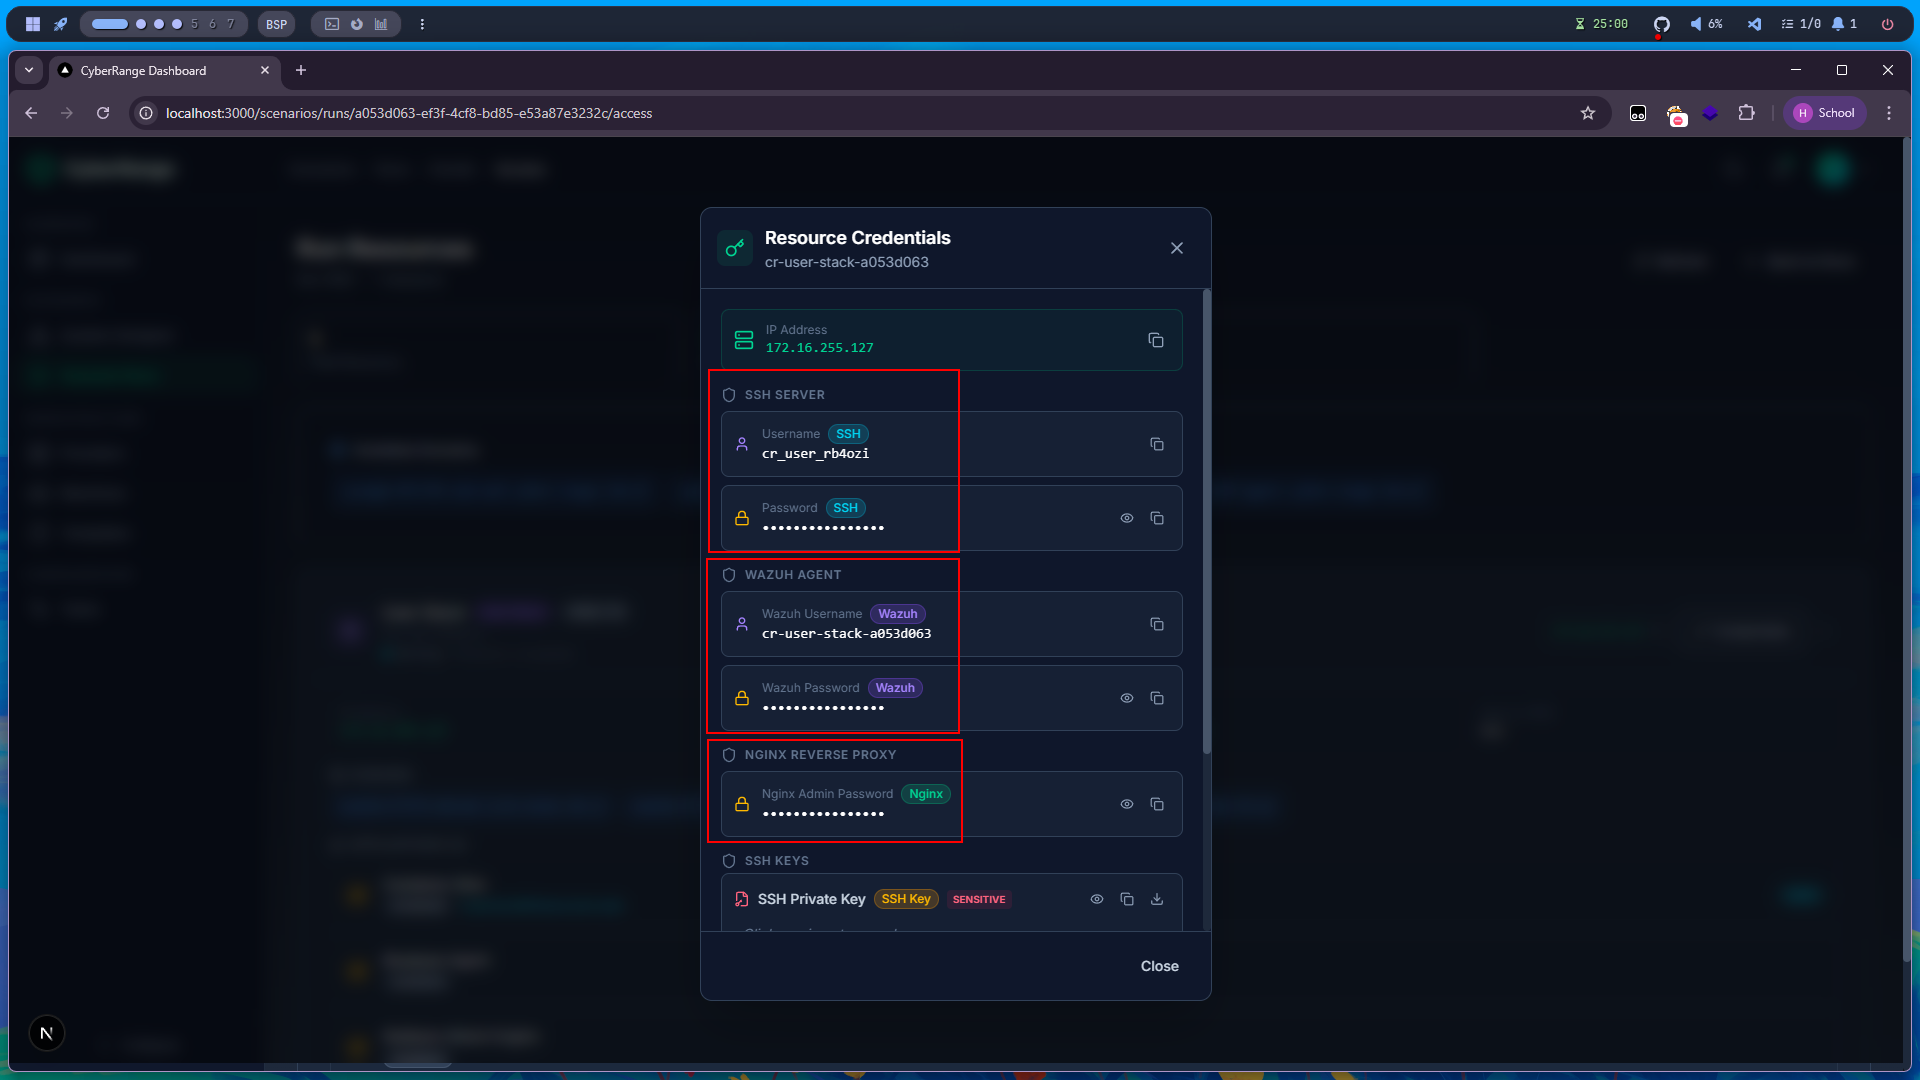
\includegraphics[width=0.95\textwidth]{images/scenarios/deploy/5.png}
    \caption{Resource credentials panel.}
    \label{fig:scenario-run-credentials}
\end{figure}

\subsection{Phase 5: Monitoring and Task Management}
The objective of this phase was to provide transparent execution observability for operators and evaluators. Core functions included task/job status tracking, log inspection, failure identification, and retry-oriented operational control.

This phase supports reliability and maintainability. By exposing execution traces and task states, it enables faster diagnosis of provisioning issues and improves confidence in repeated scenario runs. In the implemented dashboard, monitoring is not limited to SIEM review; it also includes a configuration-task layer that standardizes recurring machine automation steps such as Docker installation, SSH hardening, monitoring deployment, firewall setup, and reverse-proxy preparation.

The configuration-task workflow provides the following control benefits:

\begin{enumerate}
    \item Centralizing reusable automation tasks so administrators can apply consistent machine setup logic across scenarios.
    \item Classifying tasks by domain such as container, security, monitoring, and web configuration.
    \item Distinguishing active and inactive tasks to reduce accidental application of incomplete automation steps.
    \item Complementing Wazuh event monitoring with infrastructure-side operational traceability.
\end{enumerate}

\begin{figure}[H]
    \centering
    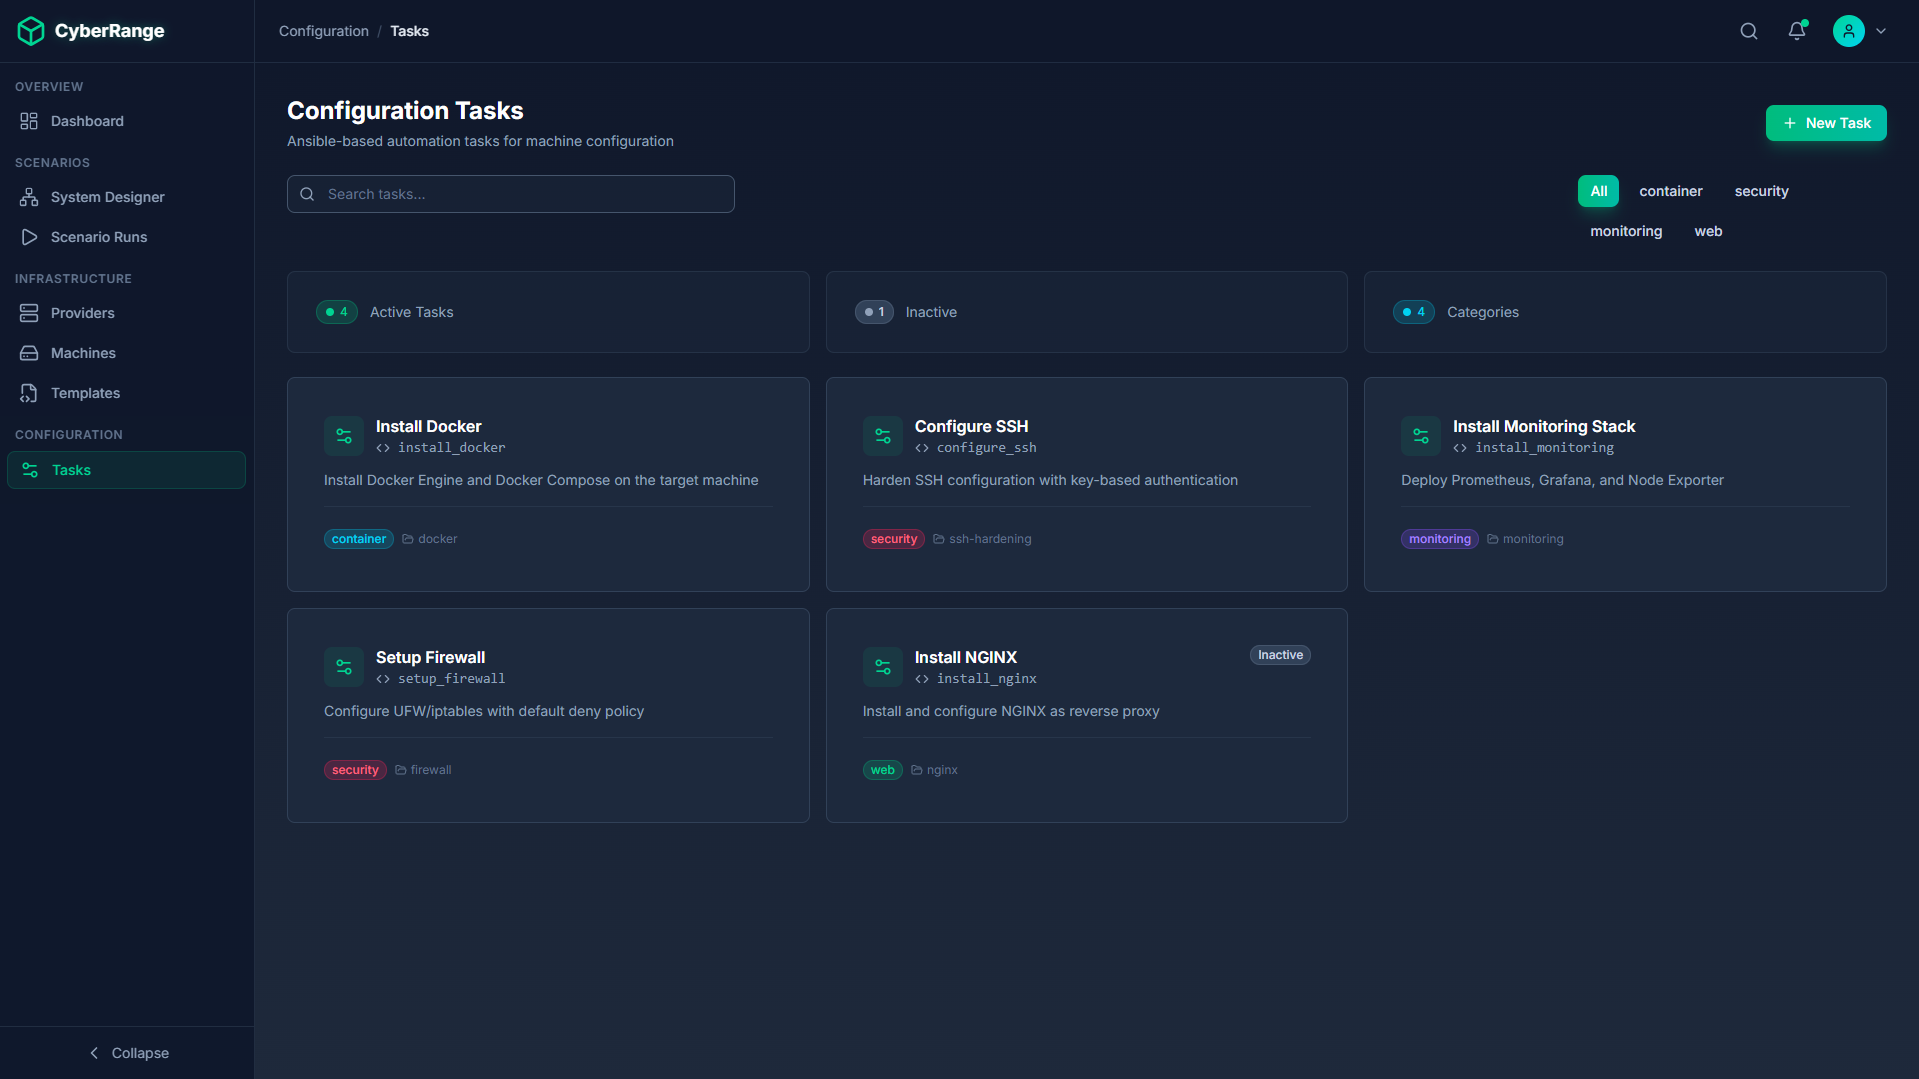
\includegraphics[width=0.95\textwidth]{images/wweb/tasks.png}
    \caption{Configuration task management.}
    \label{fig:phase5-task-management}
\end{figure}

\begin{figure}[H]
    \centering
    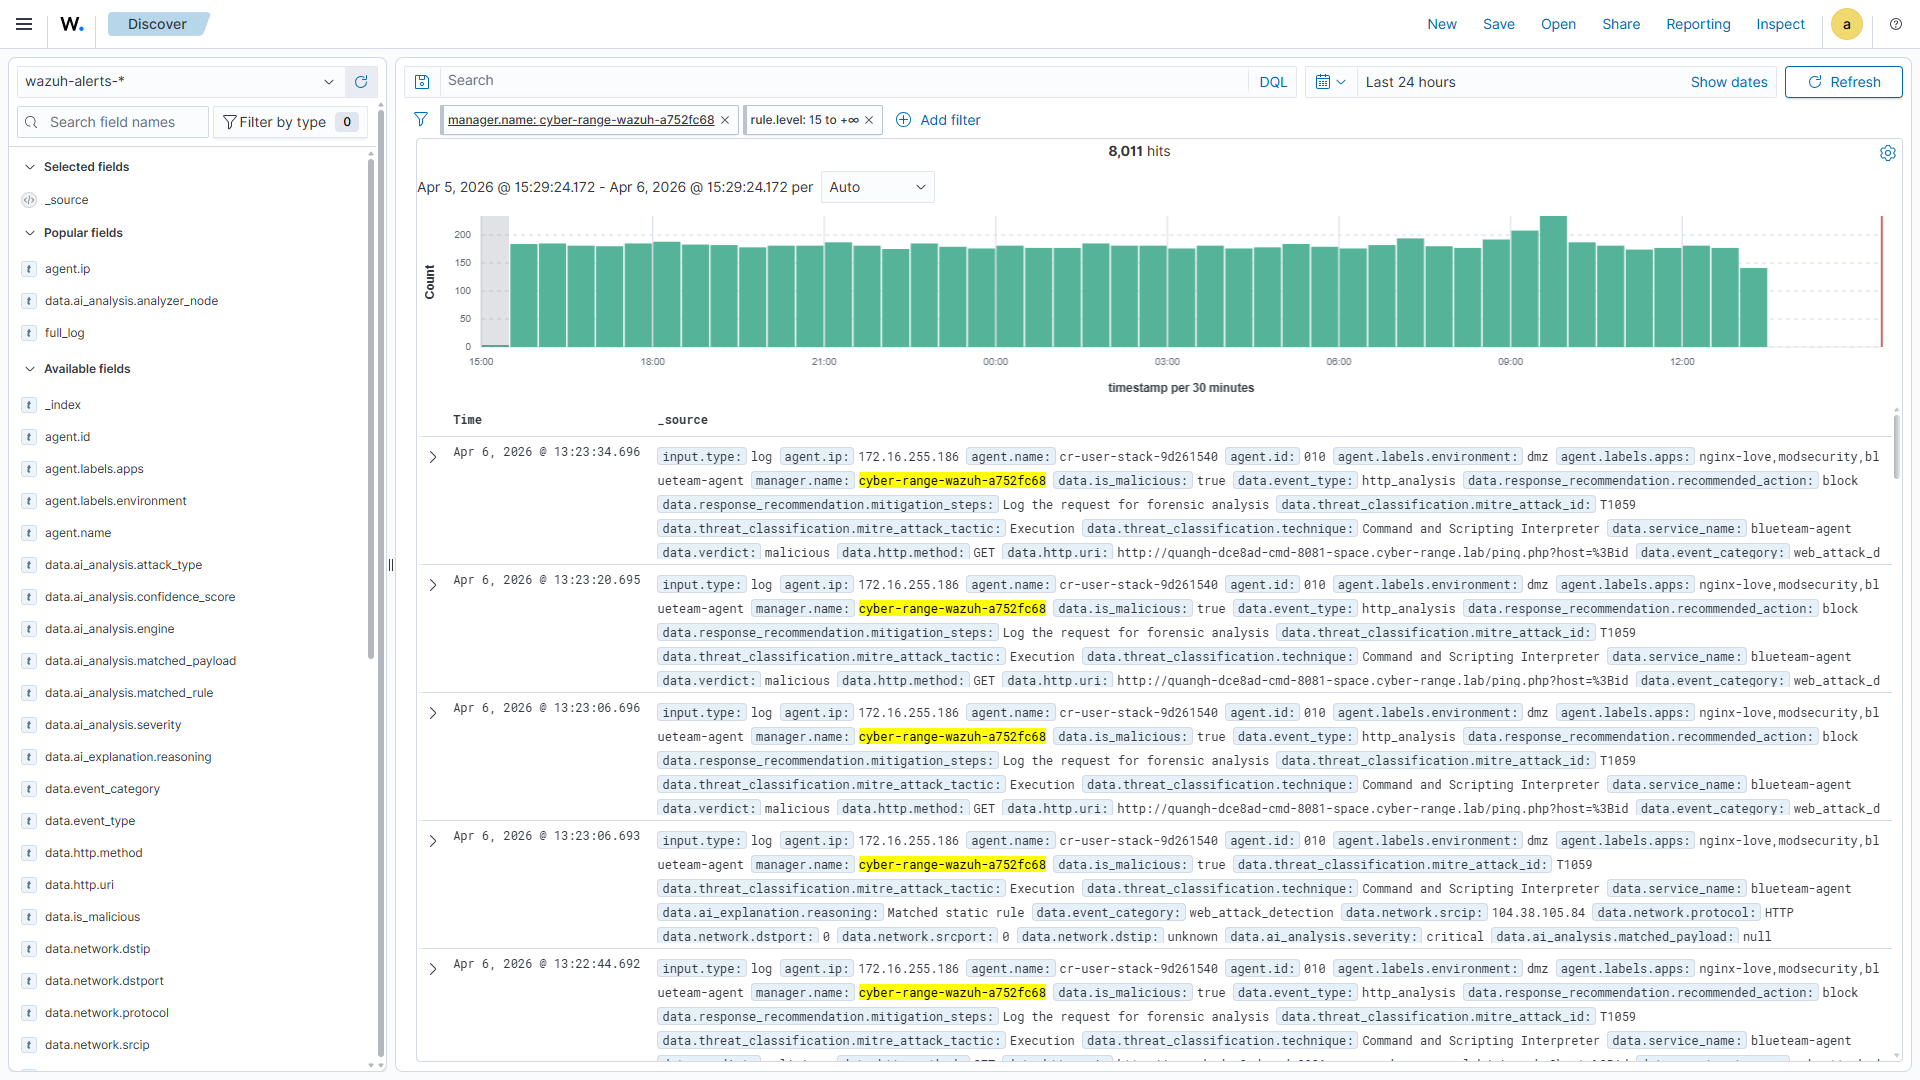
\includegraphics[width=0.95\textwidth]{images/wz.png}
    \caption{Wazuh log view.}
    \label{fig:wazuh-log-view-1}
\end{figure}

\begin{figure}[H]
    \centering
    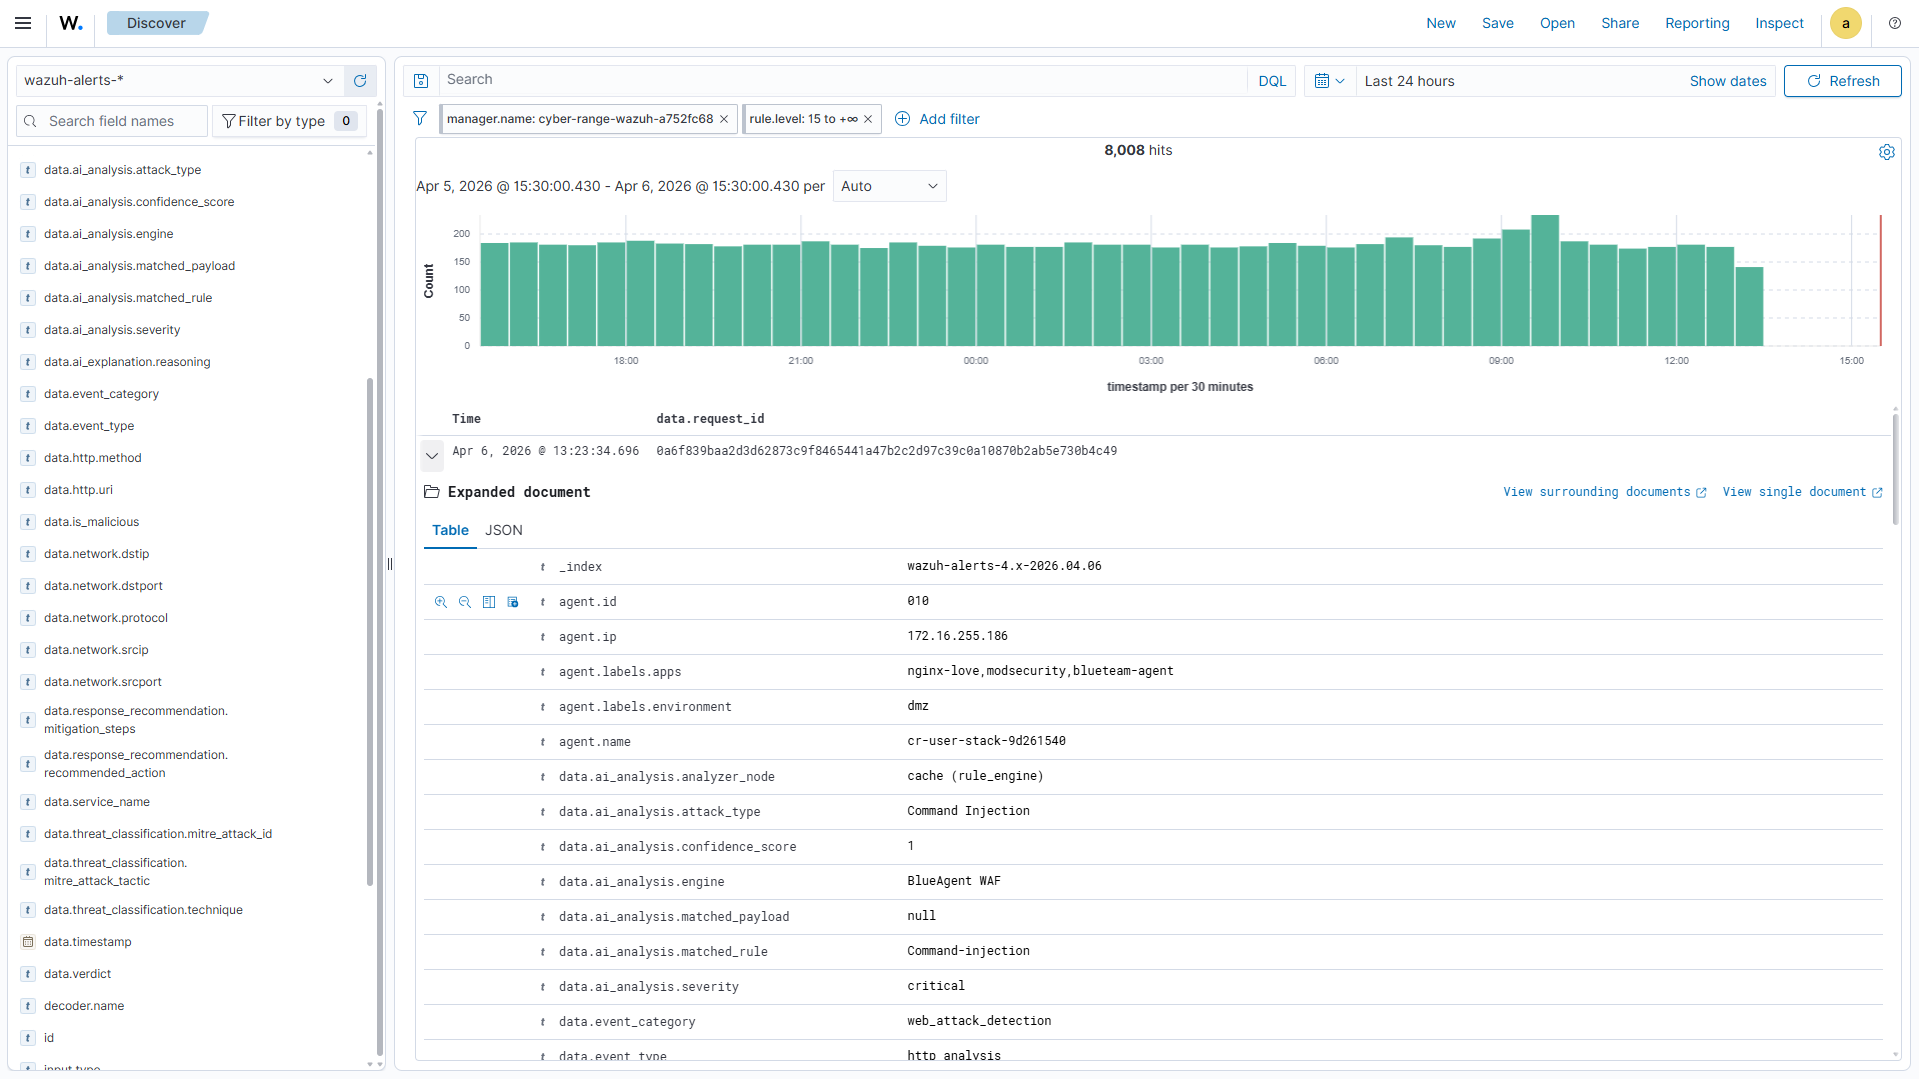
\includegraphics[width=0.95\textwidth]{images/wz1.png}
    \caption{Wazuh event details.}
    \label{fig:wazuh-log-view-2}
\end{figure}

\subsection{Phase 6: Dashboard Interaction and Visualization}
The objective of this phase was to integrate all operational capabilities into a coherent dashboard experience. Core functions included navigation across provider, template, scenario, deployment, and monitoring modules; state-aware data presentation; and role-appropriate interaction flows.

Practical usability is determined here. Even when backend services are correct, adoption in academic training depends on whether users can execute workflows efficiently through the dashboard interface.

In the implemented system, the dashboard is consolidated into a central operational overview page. This view summarizes infrastructure readiness and recent operator activity so that users can quickly assess platform state before creating scenarios or launching deployments.

The implemented dashboard workflow provides the following operational support:

\begin{enumerate}
    \item Presenting high-level platform metrics, including infrastructure providers, provisioned machines, validated templates, and active users.
    \item Exposing quick-action entry points for frequent administrative tasks such as adding providers, provisioning machines, and importing templates.
    \item Displaying recent activity events so that operators can verify successful actions, identify failed builds, and correlate changes with ongoing infrastructure work.
    \item Reducing navigation overhead by placing overview status, action shortcuts, and operational signals in one page.
\end{enumerate}

\begin{figure}[H]
    \centering
    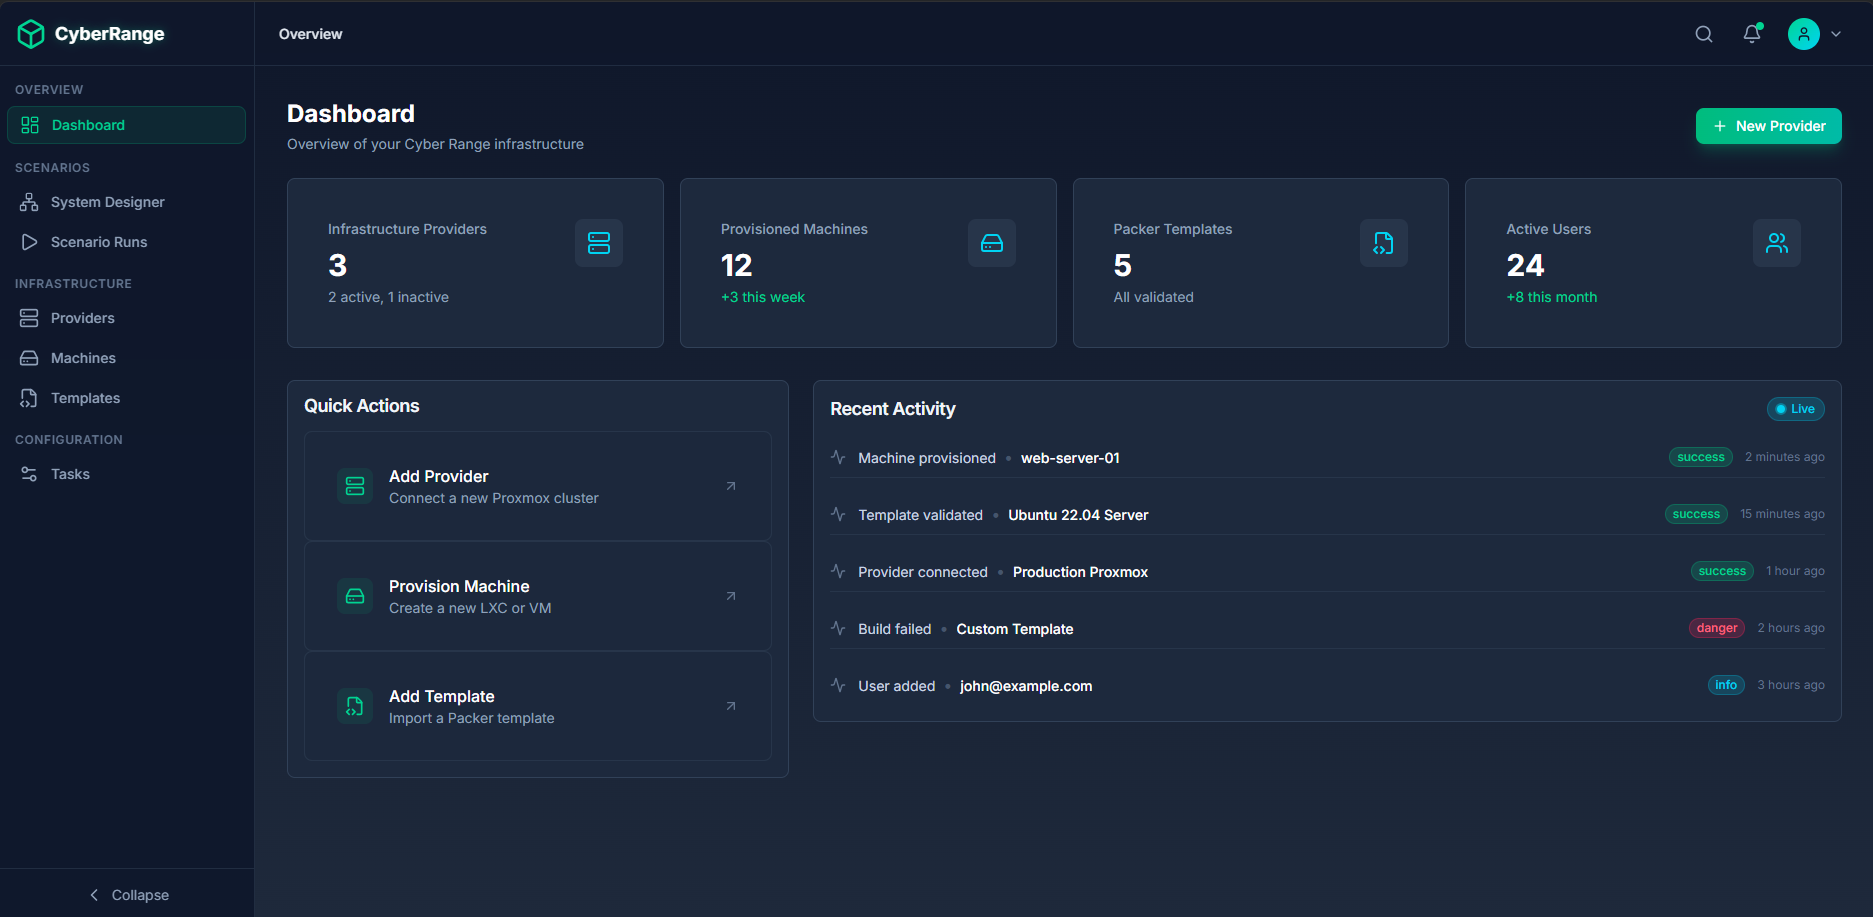
\includegraphics[width=0.95\textwidth]{images/dashboard/overview.png}
    \caption{Dashboard overview.}
    \label{fig:dashboard-overview-main}
\end{figure}

\subsection{Phase 7: AI-Assisted Analysis}
Where enabled, this phase introduced AI-assisted interpretation as an augmentation layer over system outputs. Core functions included contextual result summarization, explanatory assistance, request-level inspection, and support for training-oriented interpretation of operational or security-relevant events.

This phase plays a supporting rather than controlling role. The system remains governed by deterministic orchestration and monitored execution, while AI assistance improves interpretability and learning value. In the implemented project, the AI layer is exposed through a dedicated BlueAgent WAF console that supports request testing, alert review, and SOC-style copilot analysis in one workspace.

To improve factual grounding and reduce unsupported model responses, the project adopts a Retrieval-Augmented Generation (RAG) pattern inside the AI analysis pipeline. Rather than relying only on the internal knowledge of the language model, the system first retrieves relevant security context from a curated knowledge base and then injects that context into the final prompt. In this capstone, the retrieved context may include prior attack patterns, security explanations, rule descriptions, mitigation notes, and historical analyst guidance associated with web attacks such as SQL Injection, Cross-Site Scripting, and Path Traversal.

\subsubsection{RAG Overview}
In the context of this Cyber Range, RAG functions as an intermediate knowledge-enrichment layer between raw security events and final AI explanations. The objective is not only to classify a suspicious request, but also to provide a grounded explanation that is consistent with observed evidence and domain-specific references.

The adopted RAG architecture combines the following components:
\begin{itemize}
    \item \textbf{Input evidence:} raw HTTP requests, WAF alerts, selected SIEM fields, and request metadata collected from the training environment.
    \item \textbf{Embedding stage:} the incoming evidence and reference knowledge are transformed into vector representations using an embedding model.
    \item \textbf{Vector retrieval:} semantically similar knowledge chunks are retrieved from Qdrant based on the current request or alert.
    \item \textbf{Prompt augmentation:} the retrieved documents are merged with the observed request context and structured instructions.
    \item \textbf{Generation stage:} Gemini produces a final explanation, verdict, and mitigation-oriented interpretation using the grounded prompt.
    \item \textbf{Orchestration stage:} LangGraph coordinates retrieval, prompt assembly, fallback logic, and response formatting.
\end{itemize}

\begin{figure}[H]
    \centering
    
\includegraphics[width=0.9\textwidth]{images/RAG_pic.png}
    \caption{RAG-based analysis pipeline used in the AI-assisted security module.}
    \label{fig:rag-pipeline}
\end{figure}

\subsubsection{RAG Operational Flow}
The operational flow starts when a trainee or administrator submits a request to the BlueAgent WAF Console, or when the platform forwards a security-relevant event for interpretation. The backend first normalizes the request into a structured record that contains the request line, headers, payload fragments, WAF indicators, and scenario context. This normalization step is important because retrieval quality depends on consistent semantic representation of the evidence.

Next, the AI service generates an embedding for the normalized evidence and issues a similarity search against the vector database. Qdrant returns the most relevant knowledge chunks according to vector similarity. These chunks may describe known attack signatures, explain why a payload is suspicious, summarize WAF rule behavior, or provide mitigation advice that is useful for SOC-style training.

After retrieval, the orchestration layer filters irrelevant context, selects the top-ranked chunks, and combines them with the original request data. The final prompt therefore contains two complementary inputs: \textit{what happened in the current request} and \textit{what prior knowledge is most relevant to explain it}. Gemini then generates a grounded response that includes a verdict, confidence level, explanation, and investigation guidance. The generated output is finally returned to the dashboard for user review.

\clearpage
\subsubsection{Hybrid RAG-Based Payload Analysis Workflow}

Algorithm~\ref{alg:rag-analysis} presents the retrieval-augmented analysis workflow implemented in the system for HTTP payload inspection and security reasoning.

\begin{lstlisting}[caption={Hybrid RAG-based payload analysis workflow},label={alg:rag-analysis},basicstyle=\ttfamily\small,breaklines=true]
Input:
  raw_http_request R
  gatekeeper_model G
  vector_database V
  dense_embedding_model M
  sparse_retrieval_model B
  language_model L

Output:
  structured_security_analysis A

1. Parse R into structured HTTP components:
     method, URL, headers, and body
2. Extract user-controlled values from:
     URL path, query parameters, headers,
     cookies, form fields, and JSON body fields
3. Normalize extracted values into payload candidates P
4. Apply gatekeeper model G to identify suspicious payloads P_s
5. For each suspicious payload p in P_s:
     a. Encode p using dense embedding model M
     b. Construct a sparse BM25 query using model B
     c. Query vector database V using hybrid retrieval
        combining dense and sparse search
     d. Fuse retrieval results using reciprocal rank fusion (RRF)
6. Merge, deduplicate, and rank retrieved results
7. Select top-k payload intelligence snippets as context C
8. Construct augmented prompt P from:
     - suspicious payloads P_s
     - retrieved context C
     - analysis instructions
     - structured JSON output schema
9. Invoke language model L with prompt P
10. Generate verdict, attack classification, confidence,
      reasoning, and mitigation guidance
11. Return structured analysis A to the dashboard
\end{lstlisting}

From an implementation perspective, this workflow integrates hybrid retrieval over a Qdrant-based payload intelligence collection before invoking the language model. The retrieval stage combines dense semantic embeddings and sparse BM25 matching, followed by reciprocal rank fusion to improve relevance.

The retrieved context consists of known malicious payload patterns and labeled attack examples, which grounds the language model's reasoning in concrete evidence. This design reduces hallucination risk and improves both analytical accuracy and pedagogical value, making the system suitable for CyberRange training scenarios where explainability and contextual understanding are critical.

It should be noted that the vector database is constructed in an offline indexing phase, where payload intelligence data is normalized, embedded, and stored for efficient hybrid retrieval during inference.

To activate AI features, administrators configure Gemini integration from \texttt{Configuration $\rightarrow$ System Settings}. This workflow allows users to securely register API keys and manage global integration parameters used by AI-enabled agents.

\begin{enumerate}
    \item Open \texttt{System Settings} and select \texttt{New Setting}.
    \item Set \texttt{Category} to \texttt{ai} and define key name as \texttt{GEMINI\_API\_KEY}.
    \item Paste the Gemini API key in the \texttt{Value} field and provide a short description for maintenance.
    \item Enable \texttt{Active} to use this setting at runtime.
    \item Enable \texttt{Secret Value} so the key is stored encrypted in the database.
    \item Save the setting and verify it appears in the AI settings list.
\end{enumerate}

Once configured, the AI analysis console supports the following workflow:

\begin{enumerate}
    \item Select a quick test preset such as SQL Injection, Cross-Site Scripting, Path Traversal, or benign traffic.
    \item Submit a raw HTTP request to the analysis workspace for inspection.
    \item Allow the AI engine to return verdict, confidence, and explanation payloads for training interpretation.
    \item Use the same interface as a SOC copilot surface for guided investigation of request behavior and WAF outcomes.
\end{enumerate}

\begin{figure}[H]
    \centering
    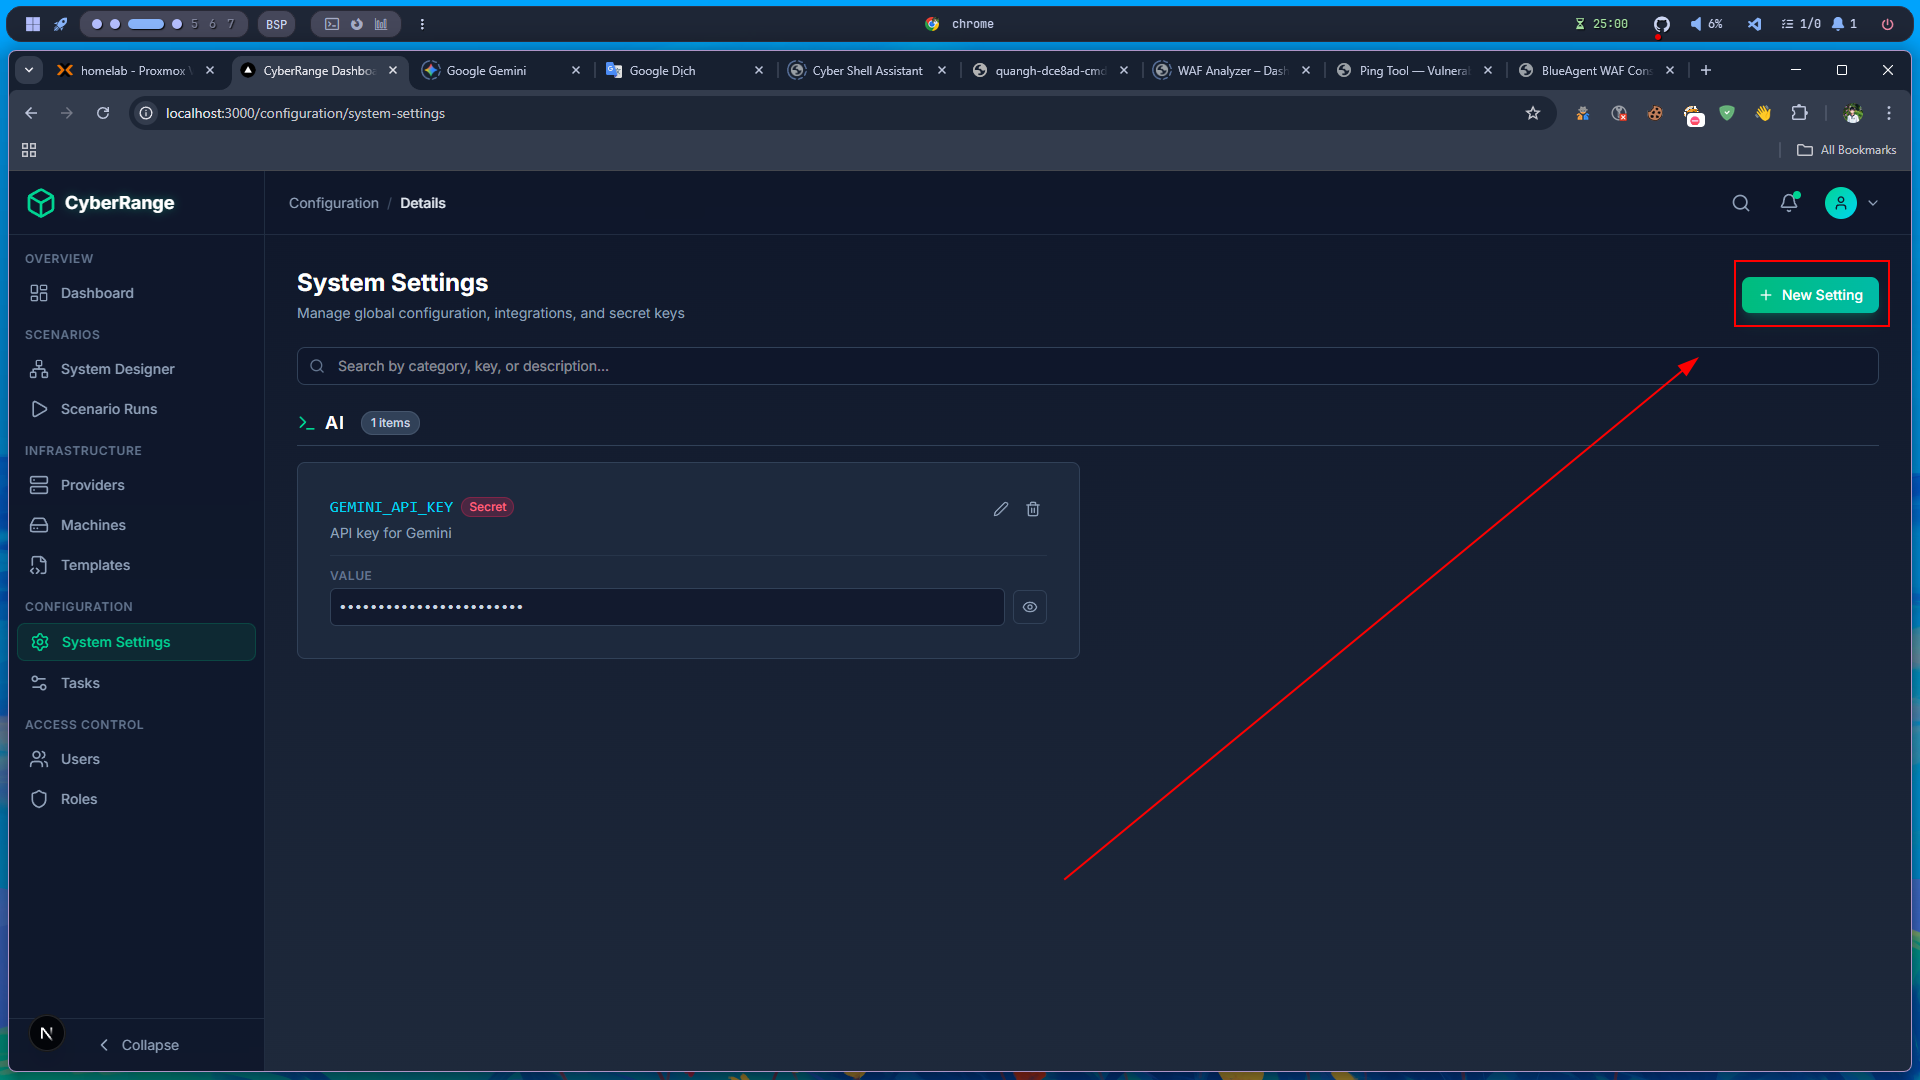
\includegraphics[width=0.95\textwidth]{images/settings/1.png}
    \caption{System settings view.}
    \label{fig:settings-gemini-list}
\end{figure}

\begin{figure}[H]
    \centering
    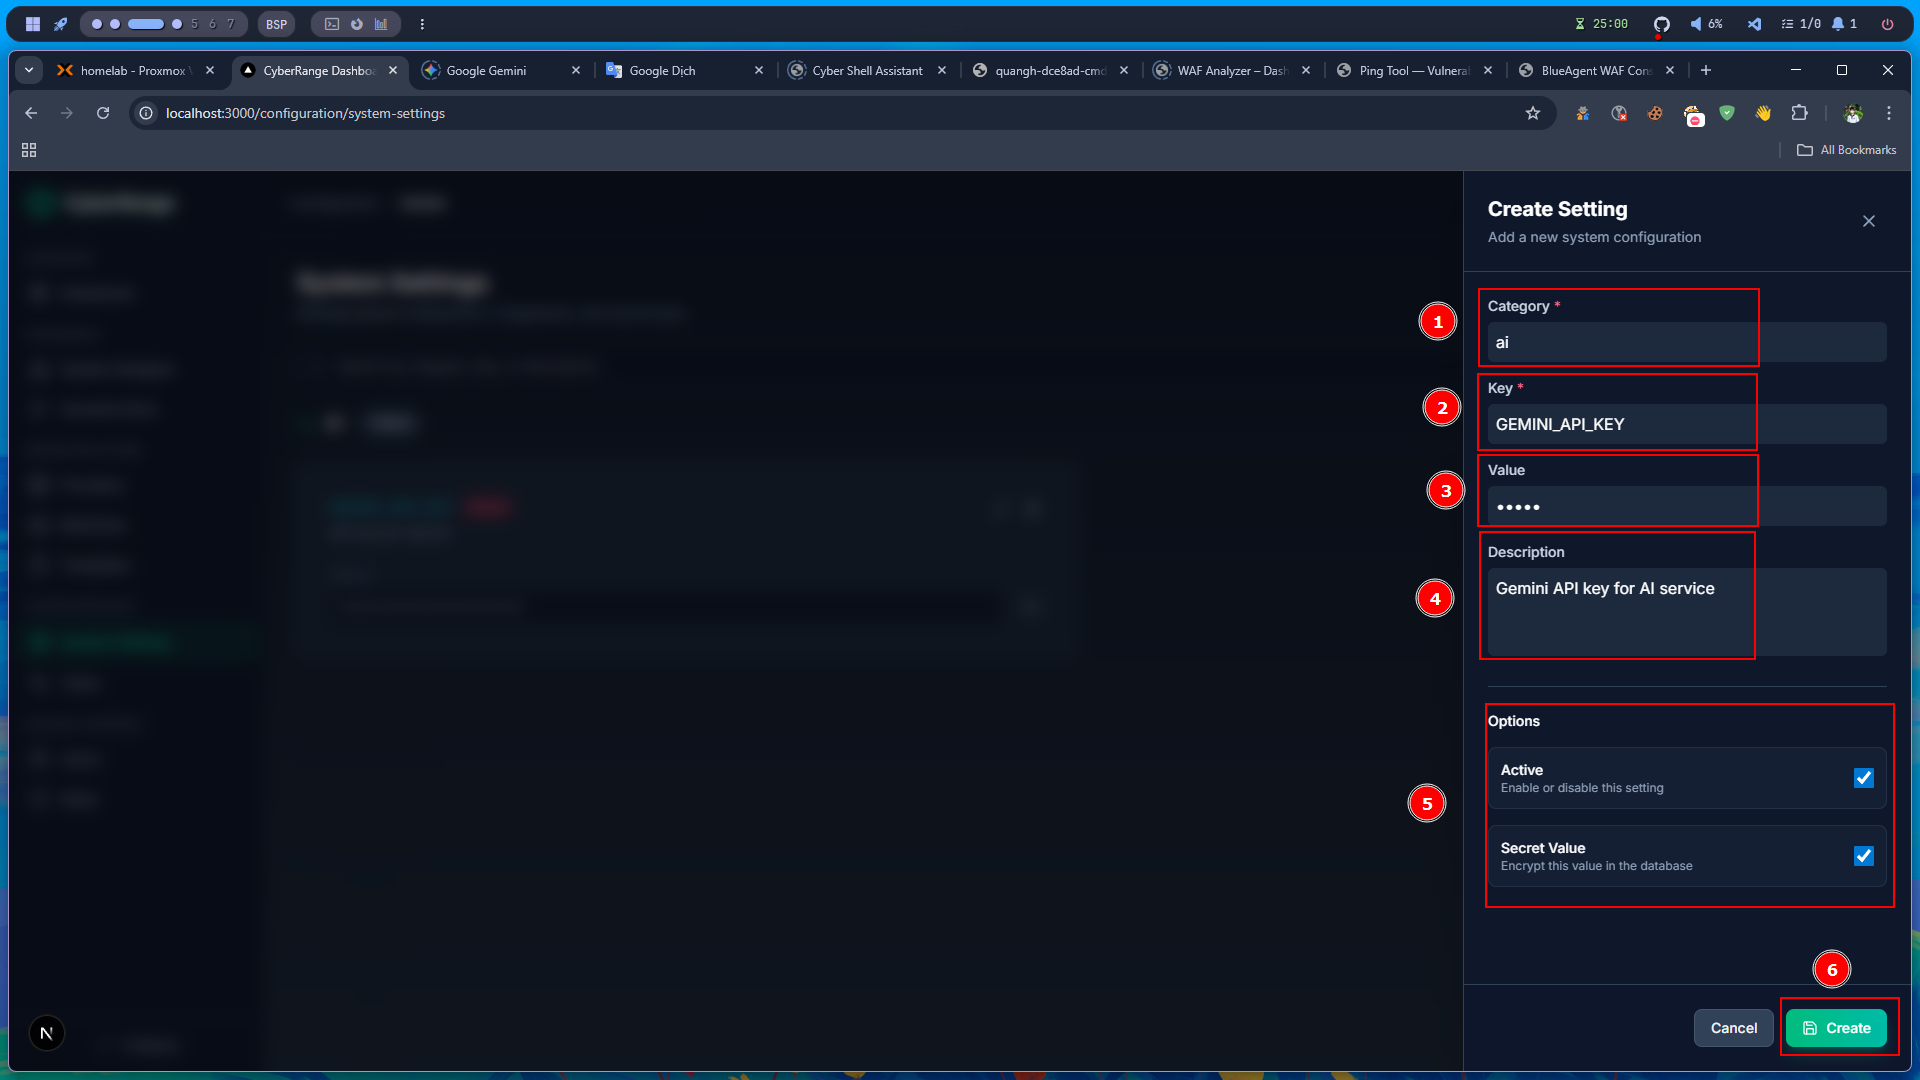
\includegraphics[width=0.95\textwidth]{images/settings/2.png}
    \caption{Gemini key setup form.}
    \label{fig:settings-gemini-create}
\end{figure}

\begin{figure}[H]
    \centering
    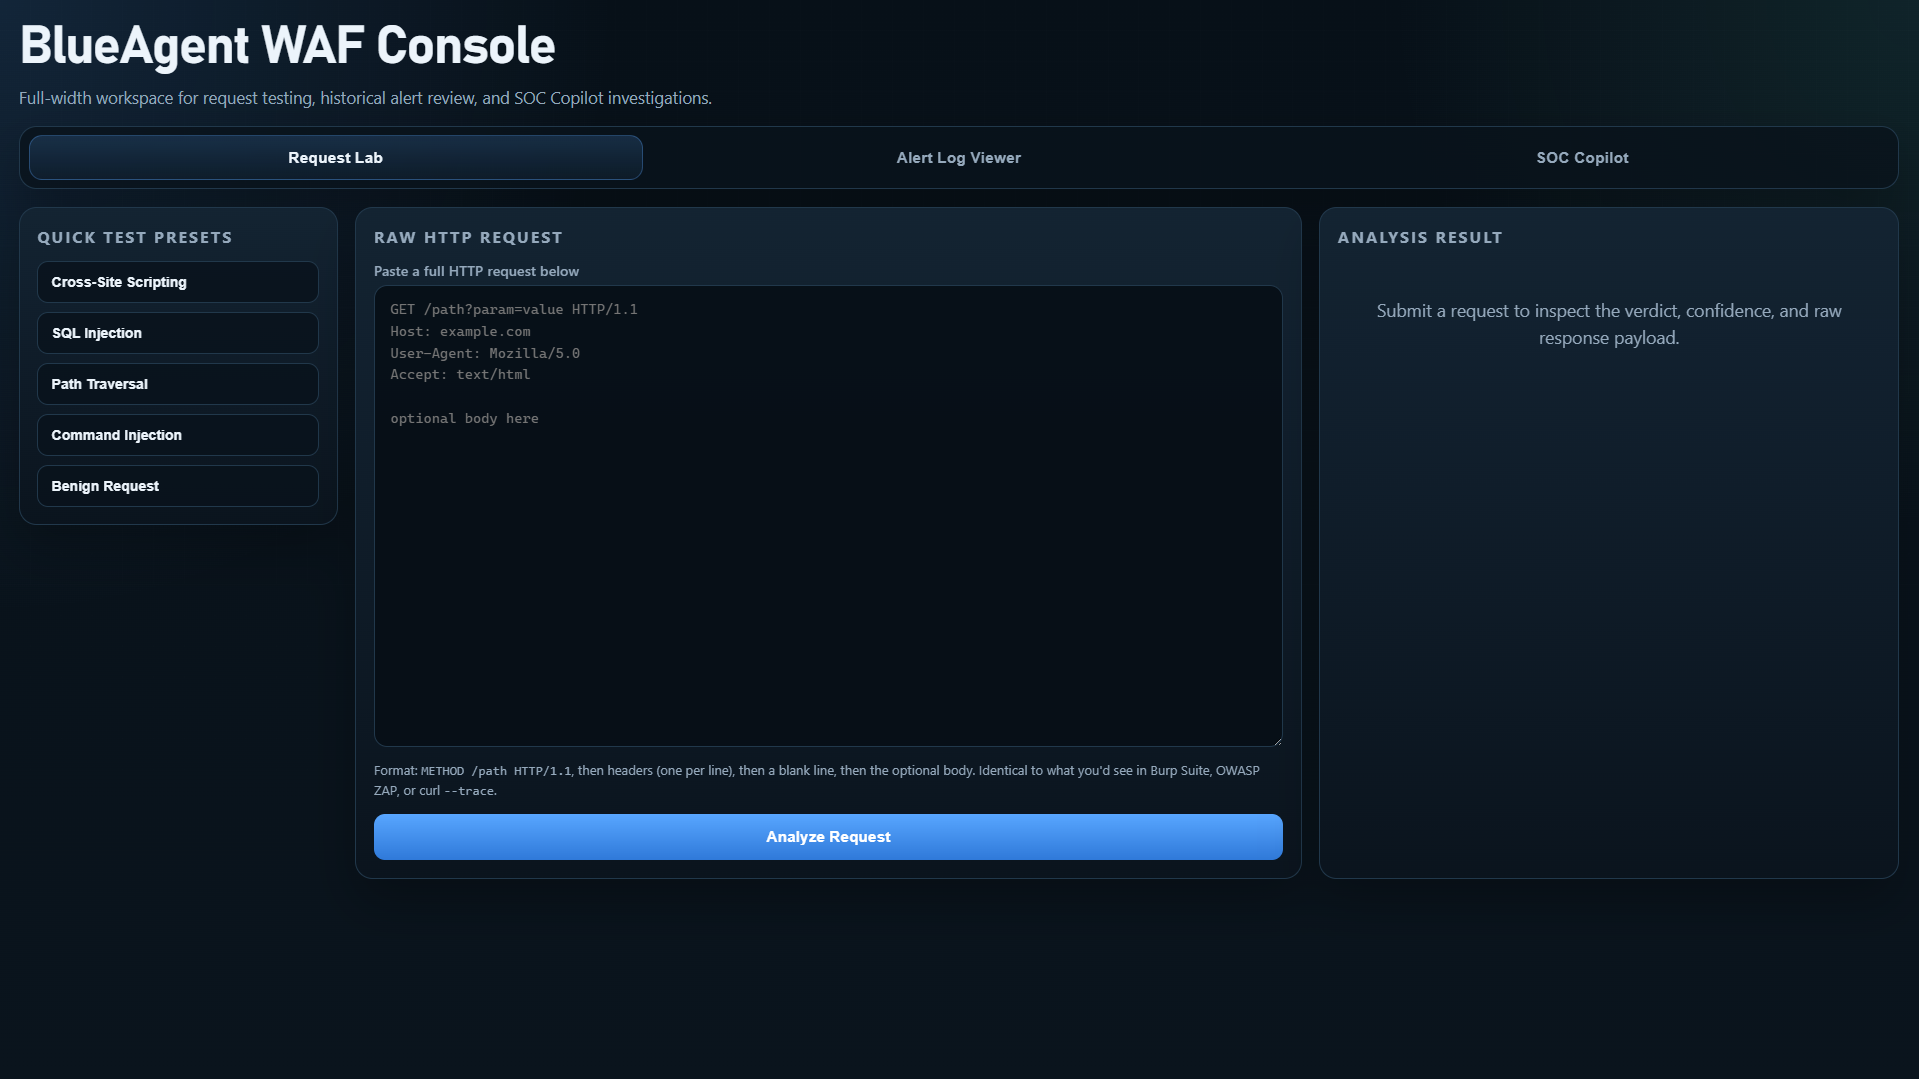
\includegraphics[width=0.95\textwidth]{images/wweb/AI analysis.png}
    \caption{BlueAgent WAF Console.}
    \label{fig:phase7-ai-console}
\end{figure}

\section{Implementation Timeline and Milestones}
\subsection{Milestone Definition}
Milestones were defined as integration-complete capabilities rather than isolated coding events. A milestone was considered achieved only when a feature could be executed from dashboard action to backend processing and observable result. This criterion ensured that progress reflected operational readiness, not only code availability.

Representative milestone groups included provider readiness, template/resource readiness, scenario lifecycle readiness, deployment orchestration readiness, monitoring readiness, and integrated dashboard readiness.

\subsection{Planned Timeline}
The timeline followed dependency order: provider setup preceded template preparation; templates preceded scenario definition; scenario definition preceded deployment validation; deployment validation preceded monitoring refinement and dashboard consolidation. AI-assisted analysis was positioned after baseline orchestration stability to ensure that interpretive features were added on top of a reliable execution core.

This sequence reduced rework, improved validation efficiency, and allowed each phase to inherit stable outputs from the previous phase.

\section{Resource and Responsibility Mapping}
\subsection{Team Responsibilities During Implementation}
Implementation responsibilities were assigned by functional domain to preserve accountability across system layers. Infrastructure-oriented responsibilities covered provider connectivity and deployment prerequisites. Application-oriented responsibilities covered scenario orchestration, task processing, and API behavior. Interface-oriented responsibilities covered dashboard workflow integrity and operational visibility. Validation-oriented responsibilities covered integration checks, defect tracking, and documentation quality.

This responsibility mapping enabled parallel work while maintaining clear ownership over cross-layer integration points.

\subsection{Infrastructure and Tooling Resources}
The implementation required resources for control services, data persistence, asynchronous task execution, and dashboard delivery. Tooling resources included provider integration utilities, template/resource management components, scenario lifecycle handlers, and monitoring/logging utilities for runtime observability.

From an academic deployment perspective, resource planning emphasized repeatability, controllability, and maintainable execution rather than maximal scale.

\section{Quality Assurance During Implementation}
\subsection{Coding and Integration Standards}
Quality control emphasized modular service boundaries, consistent API contracts, explicit error signaling, and deterministic state transitions for scenario lifecycle operations. Configuration handling and sensitive integration parameters were managed through controlled backend paths to reduce operational risk.

Integration standards required each module to expose observable outputs that could be validated through dashboard views and task logs.

\subsection{Verification and Validation Checkpoints}
Verification checkpoints were applied at the end of each phase to confirm that newly integrated capabilities remained compatible with existing workflows. Validation focused on end-to-end execution evidence: user action, backend processing, task-state progression, and observable result.

This checkpoint strategy reduced late-stage integration surprises and improved confidence in final demonstration readiness.

\section{Risks in Implementation Execution}
\subsection{Execution Risks}
Primary implementation risks included provider-connection instability, template inconsistency, scenario-definition mismatch, asynchronous job failure, incomplete observability in task logs, and user-flow ambiguity in dashboard navigation. Additional risk existed where AI-assisted outputs might be interpreted without sufficient contextual grounding.

\subsection{Mitigation Actions in Development}
Mitigation actions included staged integration, early validation of provider and template readiness, controlled scenario lifecycle testing, structured task/log monitoring, and retry-aware execution handling. Dashboard workflows were reviewed iteratively to reduce navigation ambiguity and improve operational clarity.

For AI-assisted functions, mitigation emphasized positioning AI outputs as advisory support, while retaining deterministic system control and traceable execution evidence.

	% !TeX root = ../main.tex
\chapter{VALIDATION DOCUMENT}

\section{Project Result}
The project delivered a functional Web-Based Cyber Range prototype with an operational dashboard and a validated orchestration workflow. The implemented system supports infrastructure provider management, template/resource handling, scenario definition, scenario deployment, and asynchronous task monitoring within a unified control environment. Validation activities confirm that the platform can execute its intended lifecycle from configuration to runtime observation.

Operationally, the dashboard serves as the effective control interface for managing core modules and reviewing system state. Scenario runs can be initiated and monitored through task/job status views, while logs provide execution evidence for validation and troubleshooting. These results indicate that the platform is suitable for controlled academic cyber-range exercises and capstone-level demonstration.

Where AI-assisted analysis is enabled, the platform can additionally provide interpretive support for selected outputs, improving educational usefulness without replacing deterministic workflow control.

\subsection{Validation Scope}
Validation in this project was performed across five operational layers: infrastructure readiness, reusable artifact readiness, scenario orchestration, monitoring and automation visibility, and AI-assisted interaction. Rather than validating isolated components independently, the team evaluated whether these layers could operate as a continuous dashboard-centered workflow.

The validation objective was therefore not limited to checking whether a page could be opened or a configuration could be saved. A capability was considered validated only when the related UI state, backend state, and operational outcome remained consistent with each other. This approach is suitable for the capstone context because the system is intended to be demonstrated as an integrated platform rather than as a set of disconnected tools.

This validation framing is important for the rest of the chapter because the evidence is presented as a workflow chain rather than as unrelated screenshots. Each later subsection therefore contributes one part of the same argument: that the platform can move from setup, to orchestration, to monitoring, and finally to AI-assisted interpretation in a coherent operational sequence.

\subsection{Infrastructure and Provider Validation}
The first validation checkpoint focused on infrastructure connectivity and provider persistence. The platform successfully supports registration of Proxmox-based providers, retention of connection details, and the transition of a provider record into an active configured state. This confirms that the control platform can maintain trusted provider metadata for downstream provisioning workflows.

In addition to the dashboard-side provider view, validation also considered the host-side Proxmox inventory. The Proxmox interface shows active virtual machines, containers, storage resources, and cyber-range-related workloads under the same operational node. This cross-check confirms that the dashboard abstraction is grounded in an actual virtualization environment rather than in mock state alone.

From a system-readiness perspective, this checkpoint is foundational because every later scenario and monitoring function depends on stable provider connectivity. If provider registration, persistence, or host-side consistency were unreliable, the remaining validation results would have little operational meaning.



These results validate that the platform can bridge dashboard-driven control with host-side infrastructure visibility, which is a necessary requirement for repeatable cyber-range deployment.

\subsection{Template and Machine Validation}
The second validation checkpoint focused on reusable artifacts and synchronized machine state. The system provides a dedicated template management module for registering Packer templates and a machine inventory view for confirming VM runtime state, node placement, and provisioned resource visibility.

Although the template list may initially be empty before artifact import, the interface already exposes the required operational states for validation: template registration entry, refresh behavior, and status segmentation. Likewise, the machine inventory confirms that provisioned workloads are visible through the dashboard with their VM identifiers, IP addresses, host node assignments, and running state.

This subsection matters because cyber-range deployment is only repeatable when reusable machine artifacts and runtime inventory remain aligned. In other words, the platform must not only create workloads, but also preserve enough structure for administrators to reuse templates and verify that instantiated machines match expected operational state.



These views validate that the platform can preserve reusable deployment inputs and expose synchronized machine state to operators before scenario execution begins.

\subsection{Dashboard and Orchestration Validation}
The dashboard overview page provides a concise validation summary of current platform readiness. It aggregates provider count, provisioned machines, reusable templates, and active users into one view while also exposing quick administrative actions and recent operational events.

This overview is important from a validation standpoint because it demonstrates that the system is not only able to store configuration, but also able to present recent operational outcomes in a form that supports decision-making. A user can immediately verify whether provider connectivity, machine provisioning, and template handling have already produced observable results.

In an academic demonstration setting, this kind of overview is especially valuable because evaluators typically need to assess platform state quickly. The dashboard therefore acts as both an operator surface and a validation artifact, showing that the system can communicate status clearly instead of hiding it behind isolated technical pages.


The dashboard therefore validates both usability and operational traceability, which are central to the academic value of the cyber-range platform.

\subsection{Scenario and Run Validation}
Scenario execution validation focuses on whether the system can expose the expected run lifecycle states and provide a dedicated surface for monitoring deployment outcomes. The \texttt{Scenario Runs} page confirms that the platform supports explicit state grouping such as total runs, running, pending, and failed categories, even when no active run is currently present.

From a validation perspective, an empty-state run interface is still meaningful because it demonstrates that the run-management subsystem has already been integrated into the navigation model, role workflow, and control architecture. It also confirms that deployment results are intended to be tracked through a dedicated module rather than through ad hoc logs alone.

This point is relevant because orchestration systems must be validated not only in success cases, but also in how they represent lifecycle state structurally. A clearly defined run-management surface makes later operational troubleshooting, demonstration, and repeat execution much more manageable.


This validates the structural readiness of the run-monitoring subsystem and its position in the full scenario lifecycle.

\subsection{Monitoring and Task Validation}
The monitoring layer was validated through both security-event visibility and reusable automation-task visibility. On the security side, Wazuh views demonstrate that alerts and detailed event context can be inspected after scenario activity. On the configuration side, the task management page shows reusable machine-automation tasks classified by domain, activation state, and functional purpose.

This combination is operationally important because it separates two forms of visibility: event-level observability and setup-level observability. Event-level observability helps operators inspect what happened, while setup-level observability helps them control how supporting machines are configured in a repeatable way.

Taken together, these two visibility layers strengthen the practical value of the platform. They show that the system is able not only to display what happened during an exercise, but also to preserve the operational building blocks needed to reproduce, debug, and refine later training runs.




These interfaces validate that the system provides sufficient observability for academic deployment review, operational debugging, and repeated training preparation.

\subsection{AI Feature Validation}
The AI layer was validated through configuration readiness and console-based interaction readiness. Configuration readiness is represented by the availability of active Gemini-backed integration in the system, while interaction readiness is demonstrated through the BlueAgent WAF Console workflow used for request inspection, assistant prompting, and investigation support.

This validation is especially important because the project goal is not simply to embed an LLM, but to embed it in a way that is operationally usable inside the cyber-range workflow. The console confirms that AI is exposed as an analysis aid attached to web-traffic inspection rather than as a disconnected chatbot.


\subsubsection{AI Console Step 1: Preparing an HTTP Request Sample}
The first console-level validation step checks whether the BlueAgent WAF Console can present a structured HTTP request sample for analysis. This request workspace is important because it gives the user a concrete input object to inspect before asking the AI layer for assistance. In academic validation terms, this confirms that the AI feature is grounded in observable web traffic rather than in free-form conversation alone.

\begin{figure}[H]
    \centering
    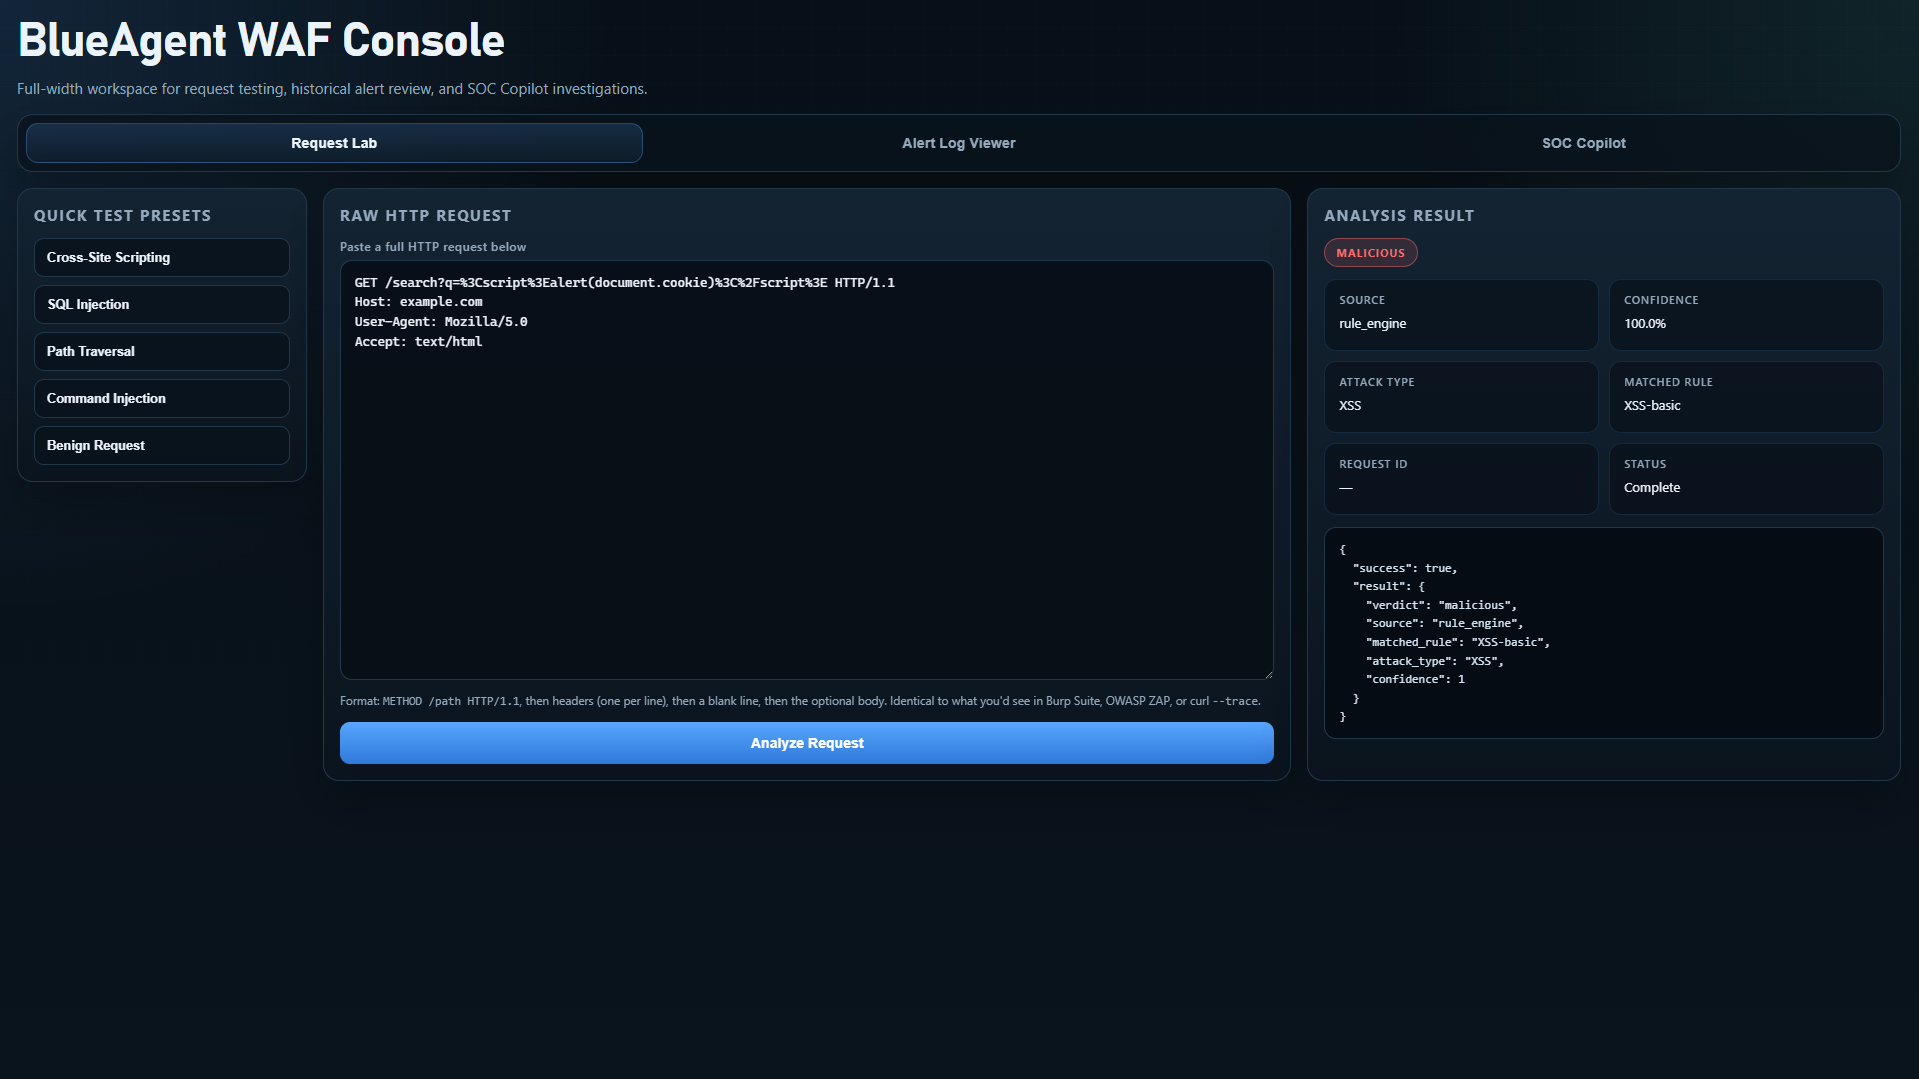
\includegraphics[width=0.92\textwidth]{images/pic/samplehttp.png}
    \caption{HTTP request sample in the BlueAgent WAF Console.}
    \label{fig:ai-console-sample-http}
\end{figure}

\subsubsection{AI Console Step 2: Sending an Analysis Prompt to the SOC Assistant}
After the request sample is available, the analyst can submit a targeted security question through the integrated SOC assistant prompt interface. This step validates that the system supports guided analyst interaction, allowing the operator to frame the investigation in a task-oriented way instead of relying only on fixed dashboard widgets. It also demonstrates that the AI layer is embedded in the same workflow used to inspect suspicious traffic.

\begin{figure}[H]
    \centering
    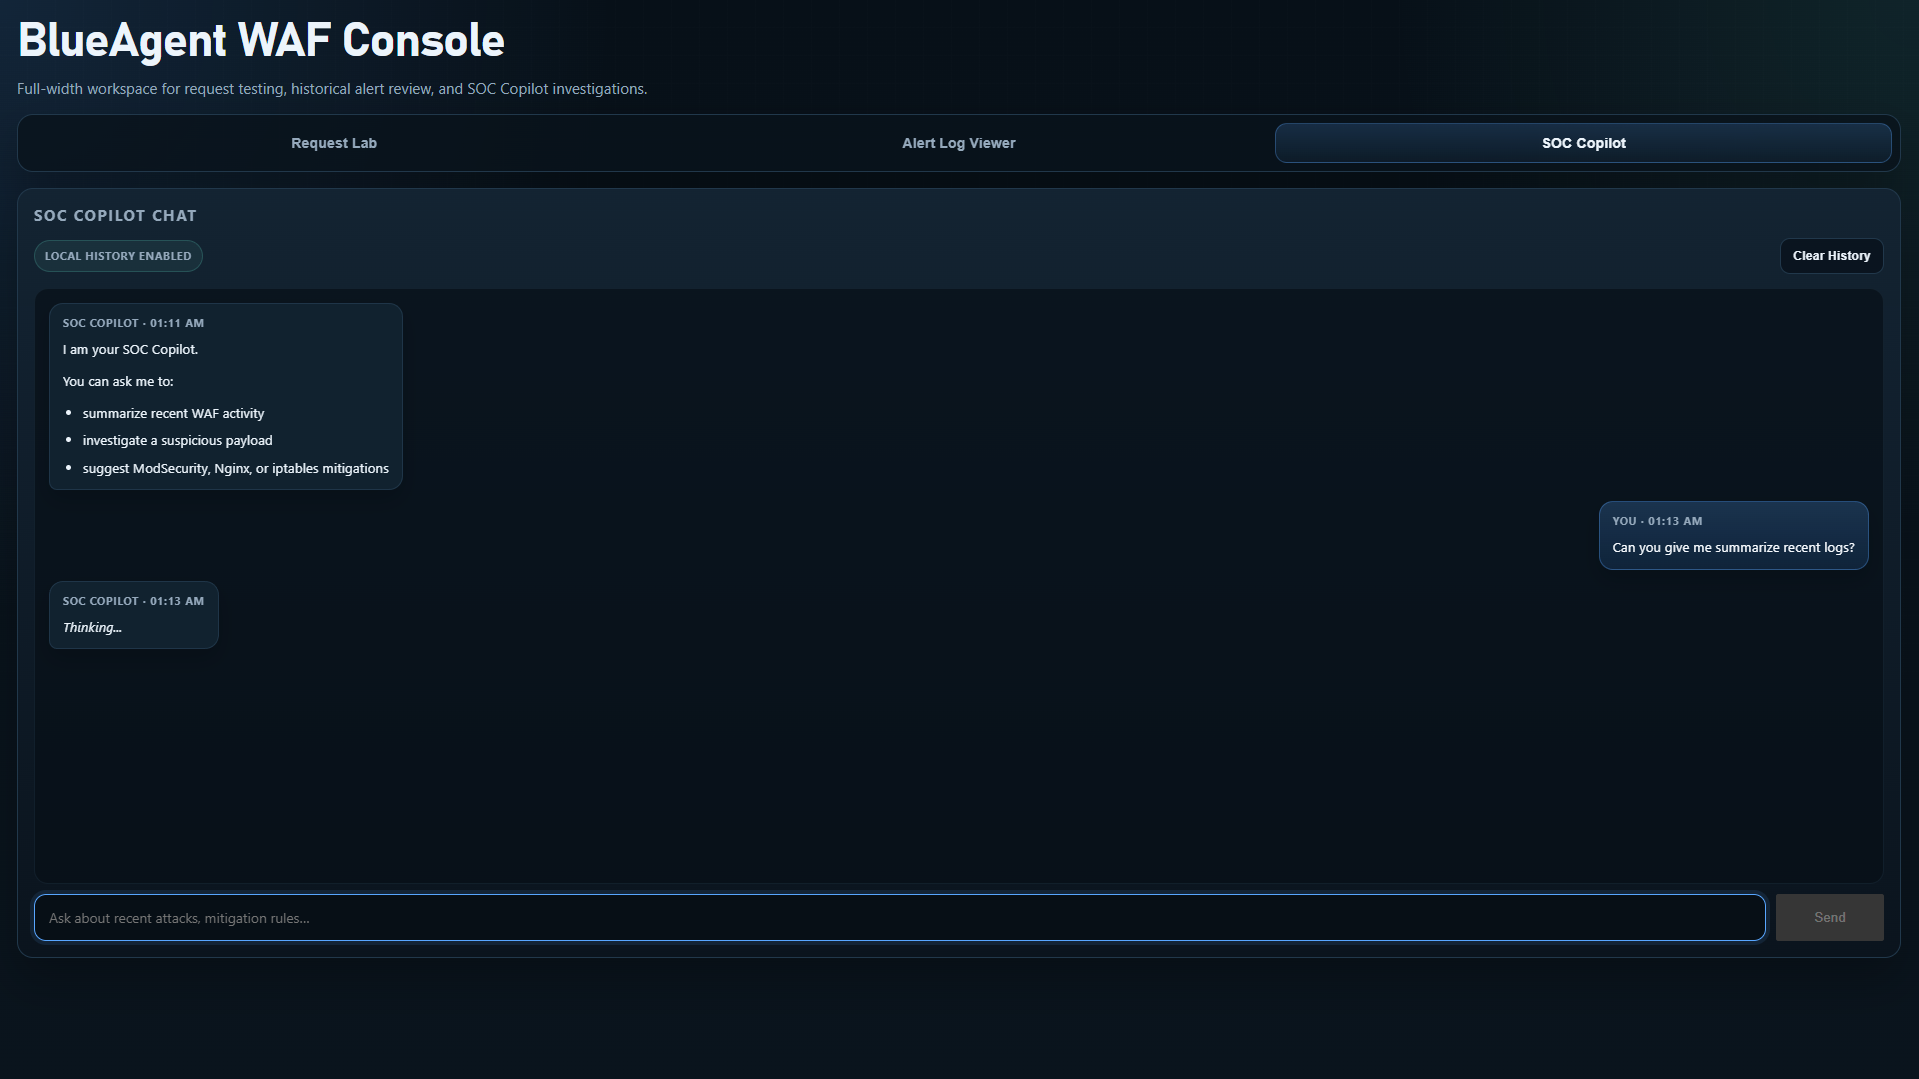
\includegraphics[width=0.92\textwidth]{images/pic/soc-ask.png}
    \caption{SOC assistant prompt in the BlueAgent WAF Console.}
    \label{fig:ai-console-soc-ask}
\end{figure}

\subsubsection{AI Console Step 3: Reviewing the Assistant's Security Interpretation}
The next validation step checks the generated AI response. The response panel shows that the SOC assistant can interpret the request content and return security-oriented observations that are usable during investigation. This matters because the aim of the feature is not only to call an LLM, but to obtain a concise explanation that helps the analyst understand why a request appears suspicious.

\begin{figure}[H]
    \centering
    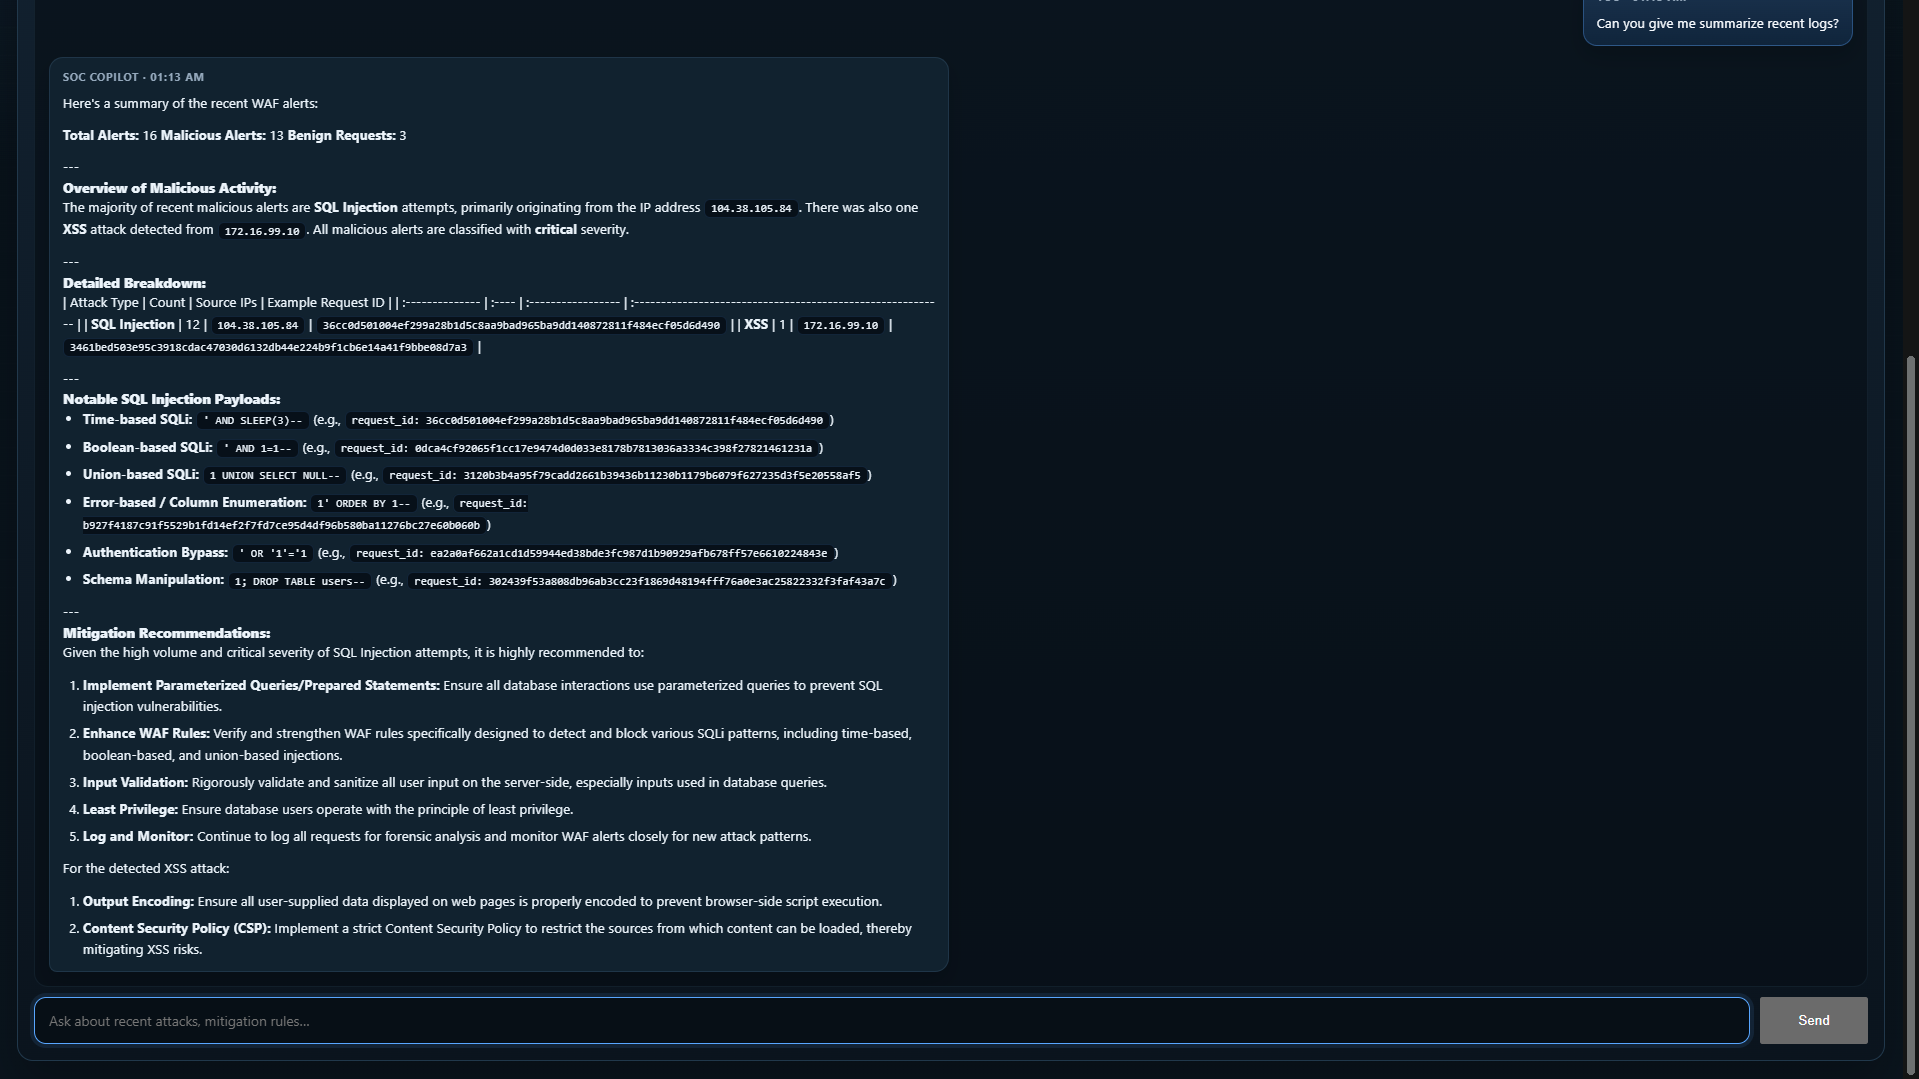
\includegraphics[width=0.92\textwidth]{images/pic/soc-answer.png}
    \caption{SOC assistant analysis output in the BlueAgent WAF Console.}
    \label{fig:ai-console-soc-answer}
\end{figure}

\subsubsection{AI Console Step 4: Using the SOC Copilot Investigation View}
The final console step validates the dedicated SOC copilot investigation view. This interface extends the earlier prompt-response interaction by presenting AI support in a more investigation-oriented layout, which is useful for analysts who need follow-up reasoning during alert review. From a validation perspective, this confirms that AI assistance is not limited to a single text response, but is integrated into a broader security-analysis workspace.

\begin{figure}[H]
    \centering
    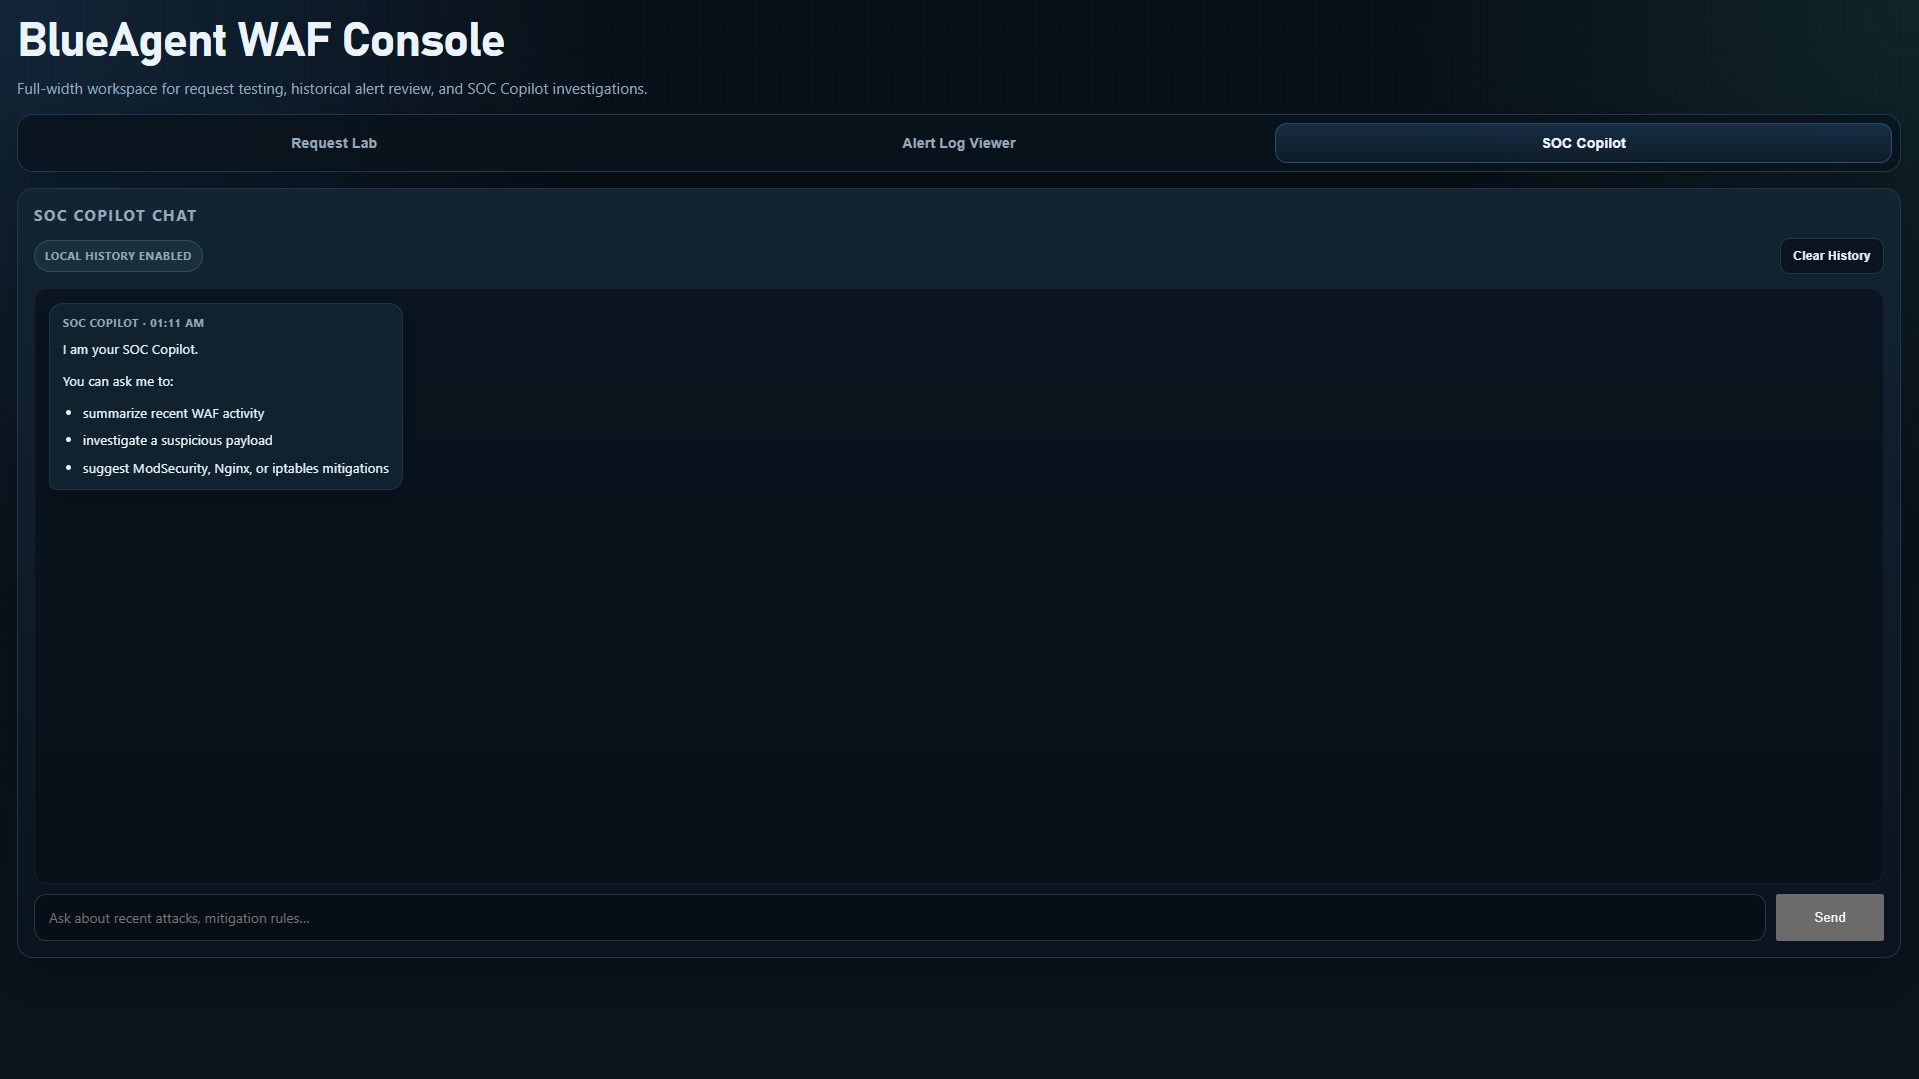
\includegraphics[width=0.92\textwidth]{images/pic/soc-coi.png}
    \caption{SOC copilot view in the BlueAgent WAF Console.}
    \label{fig:ai-console-soc-copilot}
\end{figure}




Taken together, these results validate that the platform supports both activation and practical use of AI-assisted analysis in a web-security training context.


\subsection{BlueTeam WAF Validation Workflow}
To make the BlueTeam capability assessment explicit, the project also validated a complete Web Application Firewall workflow using the BlueAgent WAF interface. In this workflow, each operational step was checked individually so that the report can show not only the final detection result, but also the configuration path that leads to that result. This is important in the capstone context because BlueTeam validation should demonstrate controllability, visibility, and investigation readiness rather than only a single alert outcome.

\subsubsection{Step 1: Accessing the BlueAgent WAF Interface}
The first step verifies that the operator can access the BlueAgent WAF through the login interface. This step confirms the availability of the defensive console and establishes the starting point of the BlueTeam workflow. From a validation perspective, successful access means that the analyst can reach the control surface used to review dashboards, inspect rules, and investigate later alerts.

\begin{figure}[H]
    \centering
    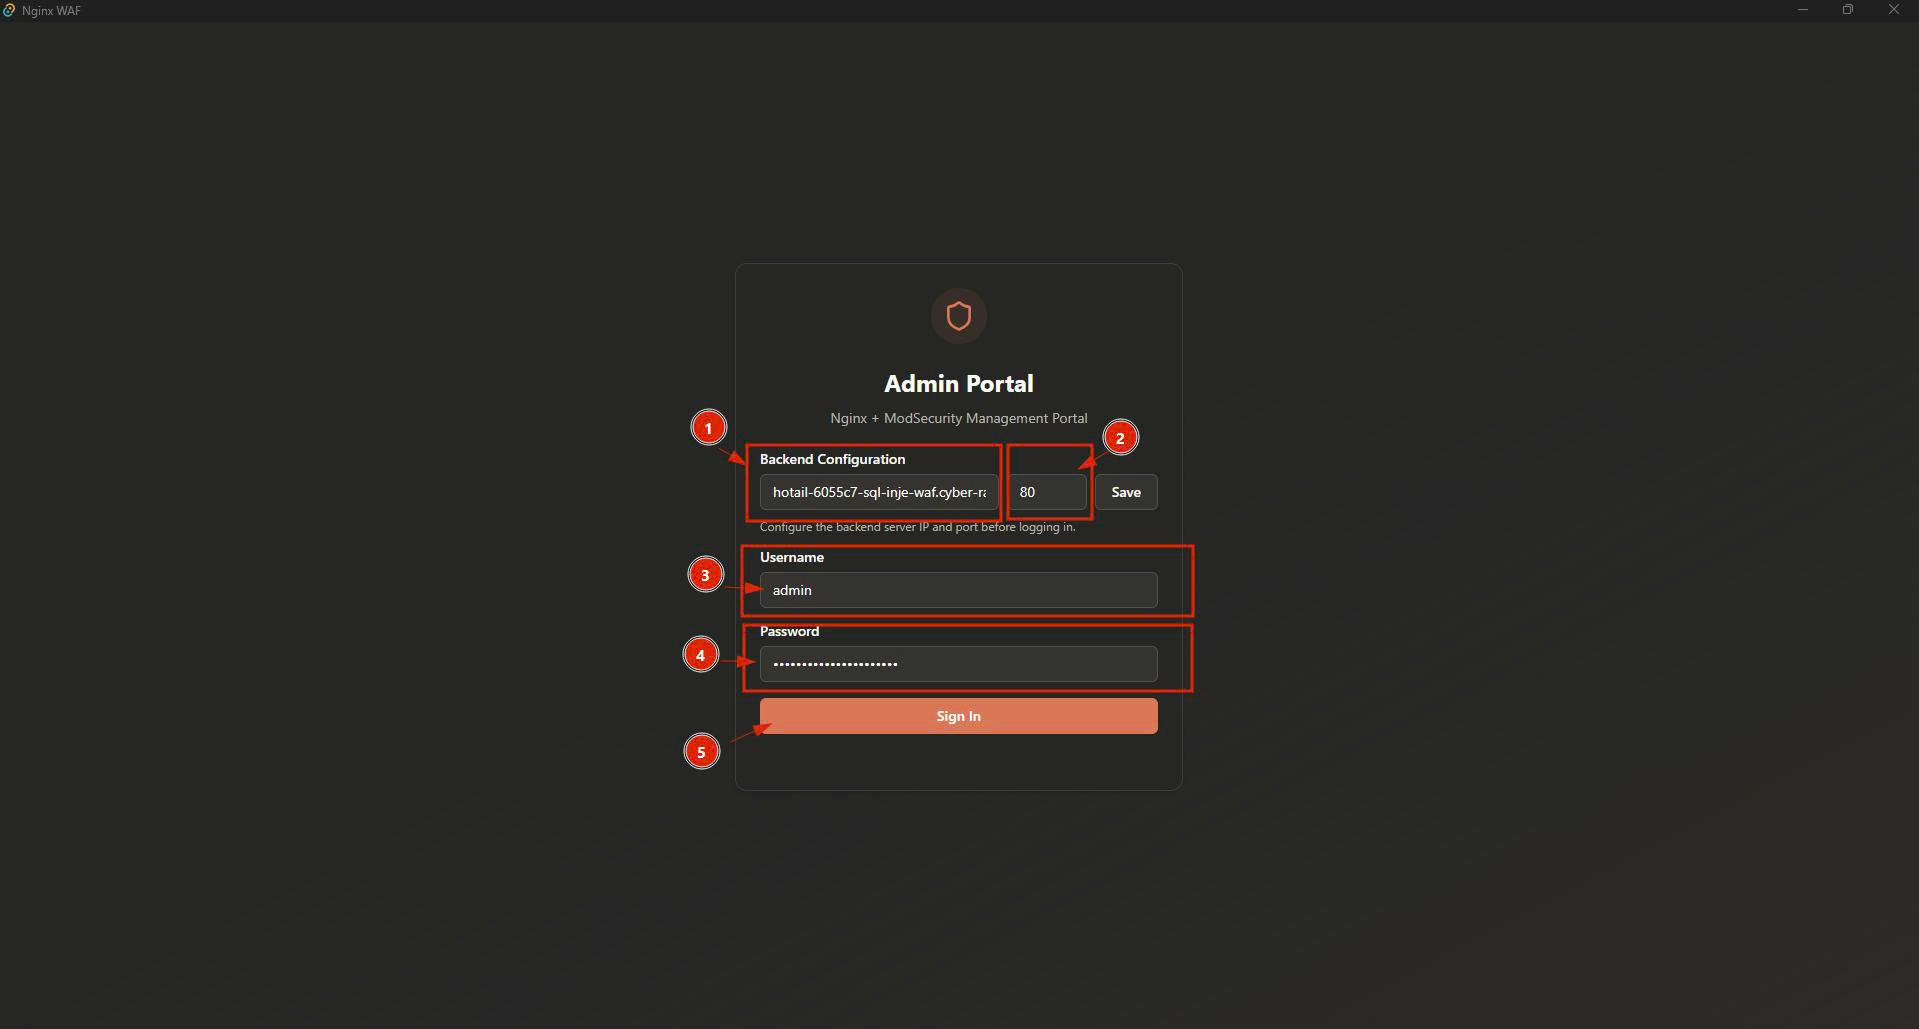
\includegraphics[width=0.82\textwidth]{images/pic/waf_login.jpg}
    \caption{BlueAgent WAF login interface.}
    \label{fig:blueteam-waf-login}
\end{figure}

\subsubsection{Step 2: Reviewing the Security Dashboard}
After successful login, the next step validates the dashboard view. The dashboard provides the BlueTeam operator with a consolidated overview of the protection system, allowing quick inspection of current security status before rule tuning or attack replay is performed. This step is useful because it shows that the platform supports operational awareness at the start of the defensive workflow rather than exposing only low-level logs.

\begin{figure}[H]
    \centering
    
\includegraphics[width=0.92\textwidth]{\detokenize{images/pic/waf dashboard.png}}
    \caption{BlueAgent WAF dashboard.}
    \label{fig:blueteam-waf-dashboard}
\end{figure}

\subsubsection{Step 3: Inspecting the SQL Injection Rule Before Activation}
The third step focuses on rule-management readiness. Before generating or replaying malicious traffic, the SQL Injection rule is inspected in its configuration interface to verify that the operator can review the relevant protection logic. This step demonstrates that the system exposes rule-level control to the BlueTeam user and that defensive behavior is not treated as a fixed black box.

\begin{figure}[H]
    \centering
    
\includegraphics[width=0.92\textwidth]{\detokenize{images/pic/rule sql.png}}
    \caption{SQL Injection rule before activation.}
    \label{fig:blueteam-sqli-rule-before}
\end{figure}

\subsubsection{Step 4: Confirming Successful SQL Injection Rule Activation}
After inspection, the SQL Injection rule is enabled and the system state is checked again. This step validates that defensive configuration changes can be applied successfully through the interface. In a BlueTeam workflow, this is a key checkpoint because the analyst must be able to move from passive observation to active protection policy enforcement.

\begin{figure}[H]
    \centering
    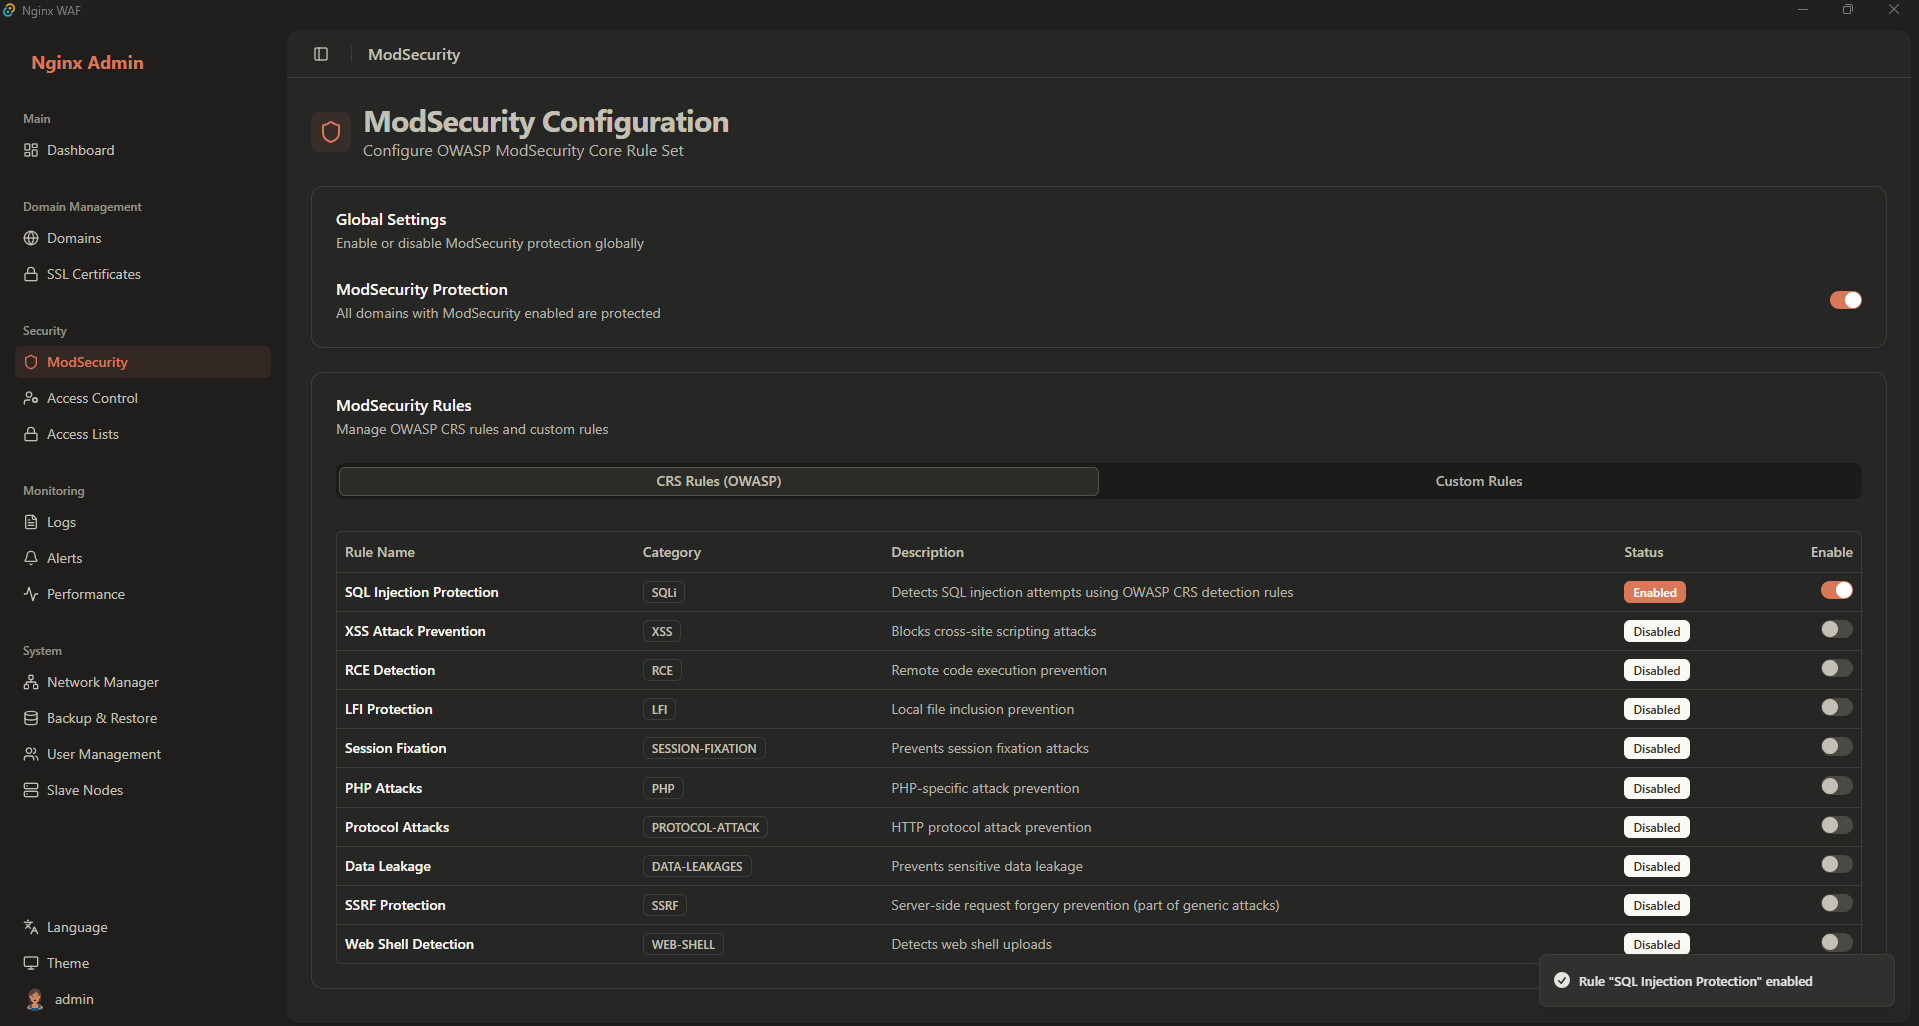
\includegraphics[width=0.92\textwidth]{images/pic/rulesqlsuccess.png}
    \caption{SQL Injection rule after activation.}
    \label{fig:blueteam-sqli-rule-after}
\end{figure}

\subsubsection{Step 5: Reviewing Security Logs After Rule Enforcement}
Once the rule is active, the validation continues by reviewing the generated security logs. This step confirms that suspicious requests are not only blocked or classified internally, but are also recorded in a way that supports later review. The captured evidence shows that the platform can present malicious web activity such as SQL Injection and XSS within the BlueTeam monitoring flow, which is essential for both training and incident analysis.

\begin{figure}[H]
    \centering
    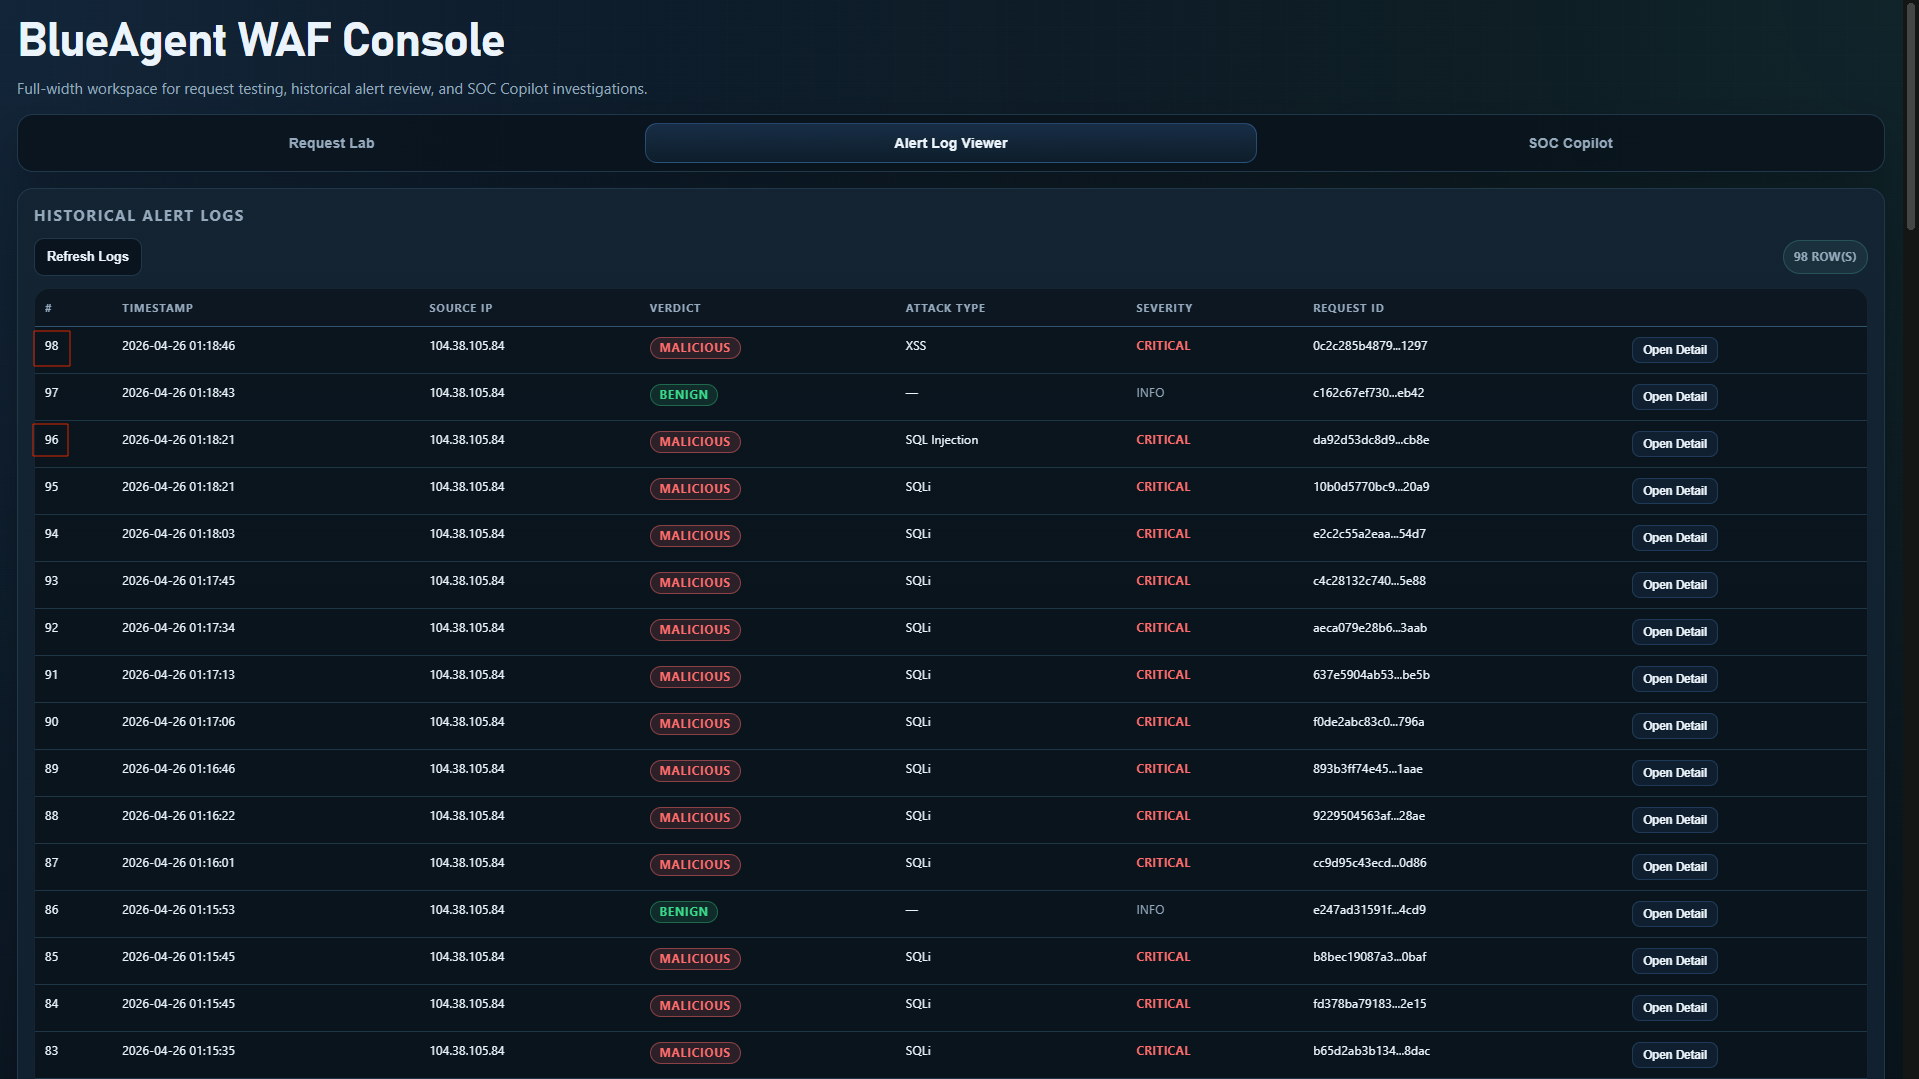
\includegraphics[width=0.92\textwidth]{images/pic/logs-rule.png}
    \caption{Security logs after rule enforcement.}
    \label{fig:blueteam-logs-rule}
\end{figure}

\subsubsection{Step 6: Investigating the Alert in Detail}
The final step validates analyst investigation capability. After a suspicious request is detected, the alert-detail view is opened to inspect the verdict, severity, attack type, source IP, HTTP method, and event payload. This is the most important evidence in the BlueTeam chain because it shows that the system does not stop at coarse alert generation; it also preserves enough context for technical interpretation and post-event analysis. The detailed JSON record strengthens the validation by proving that the platform retains structured evidence for security review.

\begin{figure}[H]
    \centering
    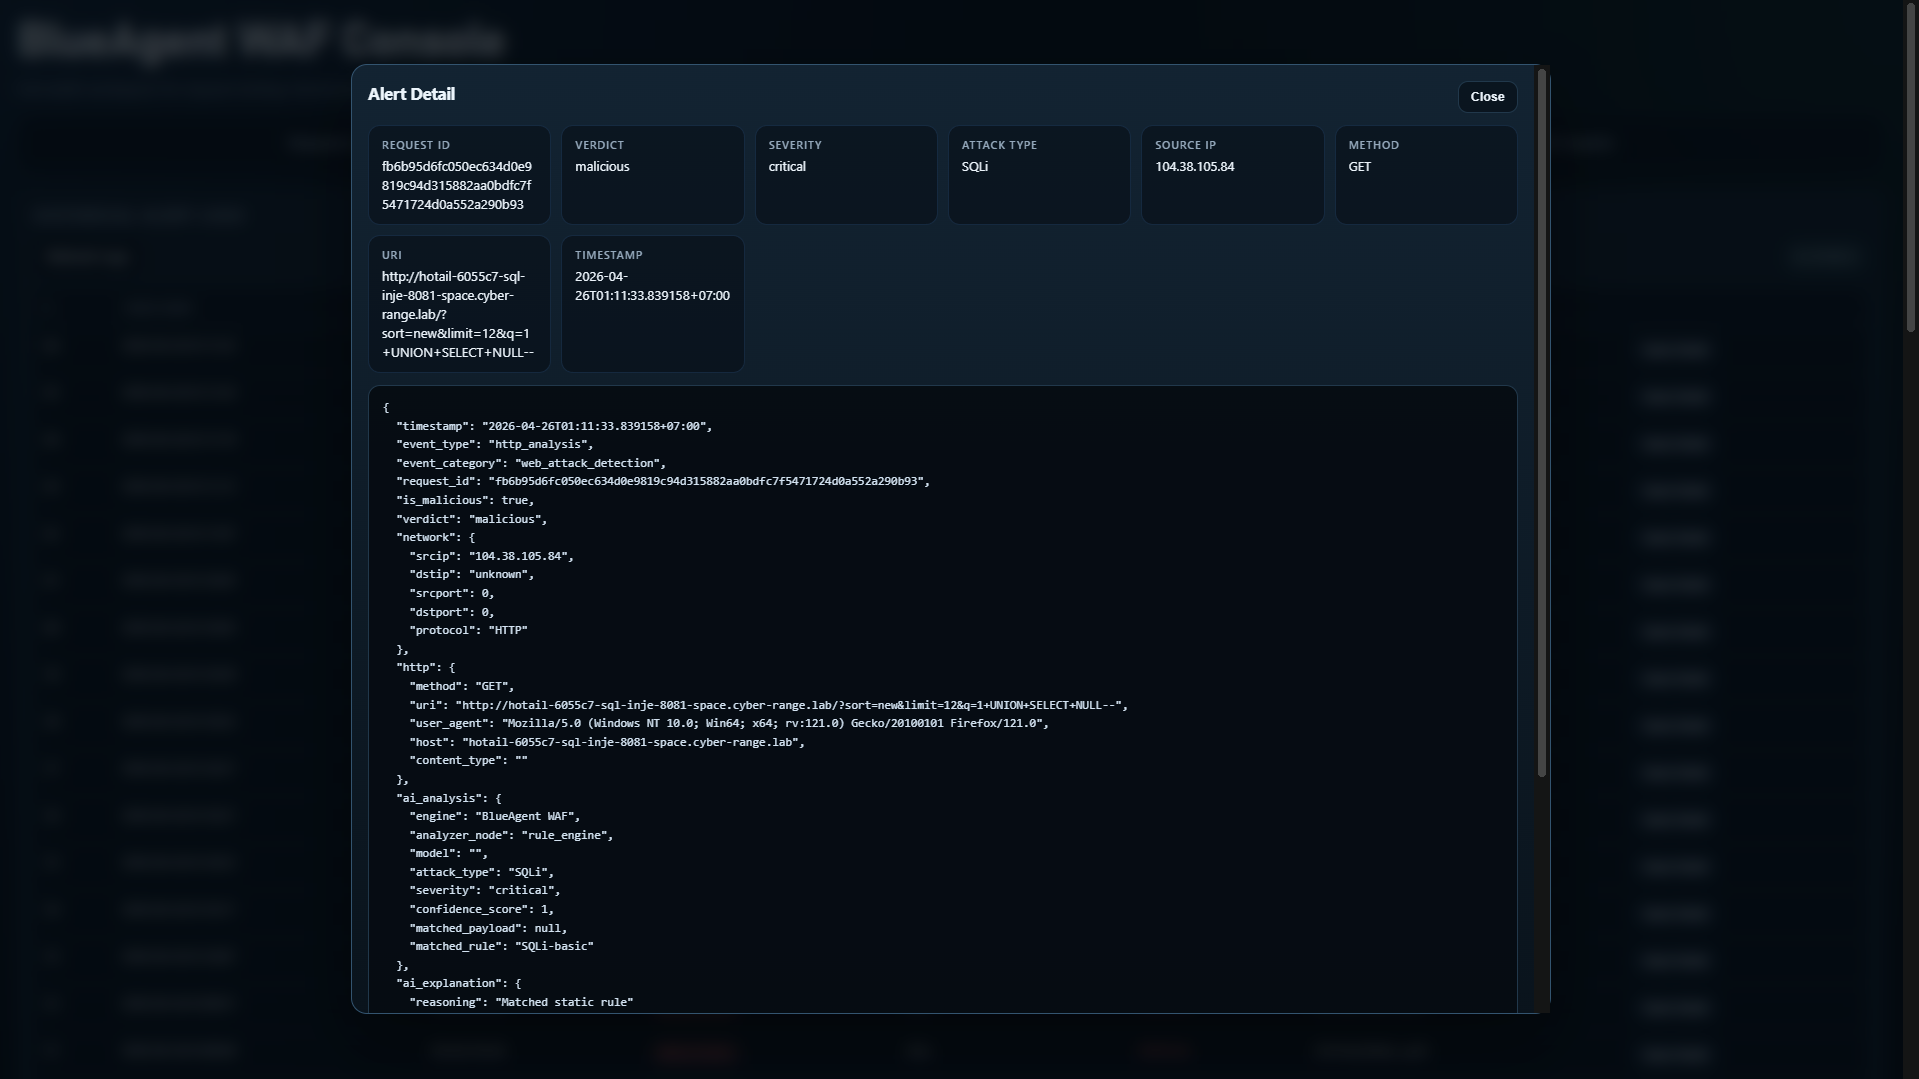
\includegraphics[width=0.92\textwidth]{images/pic/alert-detail.png}
    \caption{Detailed SQL Injection alert in BlueAgent WAF.}
    \label{fig:blueteam-alert-detail}
\end{figure}

Taken together, these six steps validate a complete BlueTeam workflow: the operator can access the defensive console, review the security dashboard, inspect and activate a protection rule, observe the resulting security logs, and investigate the generated alert in detail. Presenting each screenshot separately is important because it demonstrates operational continuity across the full defensive process rather than compressing multiple validation checkpoints into a single composite image.


\subsection{RedTeam AI-Assisted Attack Workflow}
The Red Team capability was also validated through a guided attack workflow built around the Cyber Shell Assistant and the vulnerable SQL App target. Unlike the BlueTeam workflow, which emphasizes monitoring and investigation, this Red Team workflow focuses on target discovery, session-aware assistant interaction, command guidance, and command execution against the web target. The provided PDF and screenshot sequence show that the assistant is not acting as an autonomous attacker; instead, it supports the learner by observing shell context, identifying the target, and suggesting commands that the user executes in the terminal.

\subsubsection{Step 1: Accessing the Cyber Shell Assistant}
The first step validates that the learner can access the Cyber Shell Assistant interface. This interface provides the session list, the captured shell-event history, and the chat panel used for AI-guided interaction. It serves as the main Red Team workspace for combining terminal activity with assistant feedback.

\begin{figure}[H]
    \centering
    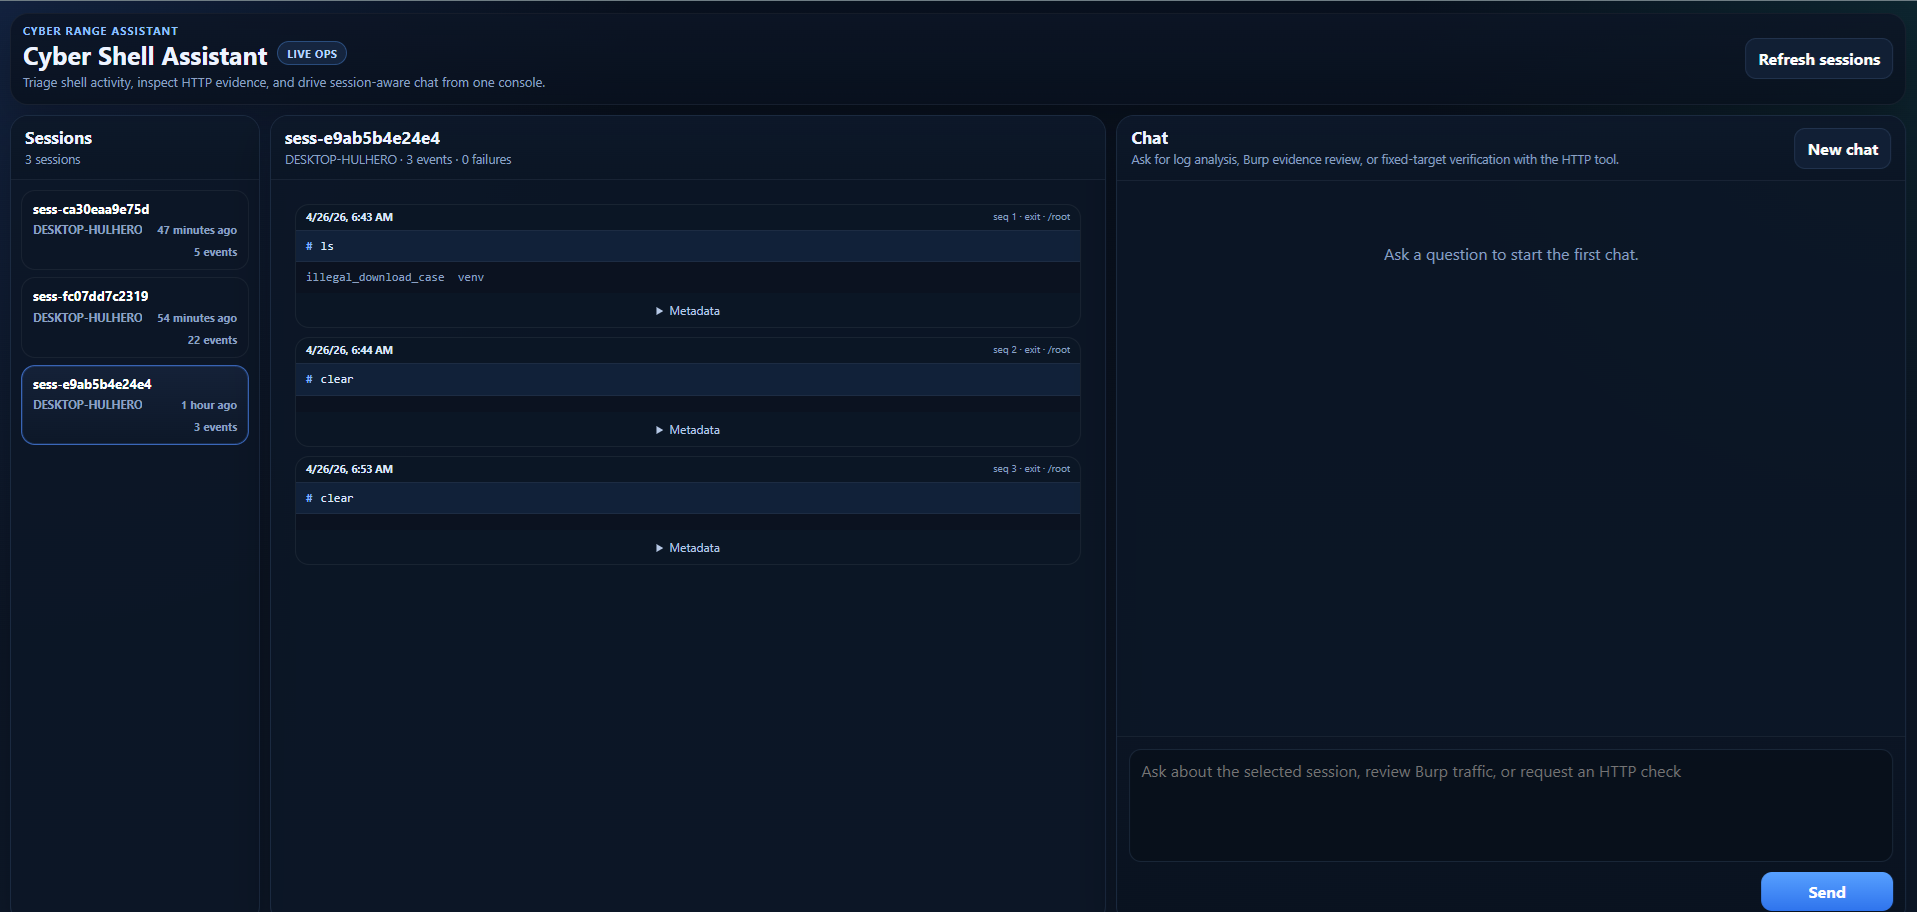
\includegraphics[width=0.92\textwidth]{images/cyred/cyred/1.png}
    \caption{Cyber Shell Assistant interface.}
    \label{fig:redteam-cybershell-interface}
\end{figure}

\subsubsection{Step 2: Opening the Target Web Application}
The second step confirms the availability of the target application used in the exercise. In this case, the learner is given access to the SQL App web target, which exposes searchable product data and becomes the focus of later SQL injection testing. This step establishes the attack surface before the learner interacts with the assistant.

\begin{figure}[H]
    \centering
    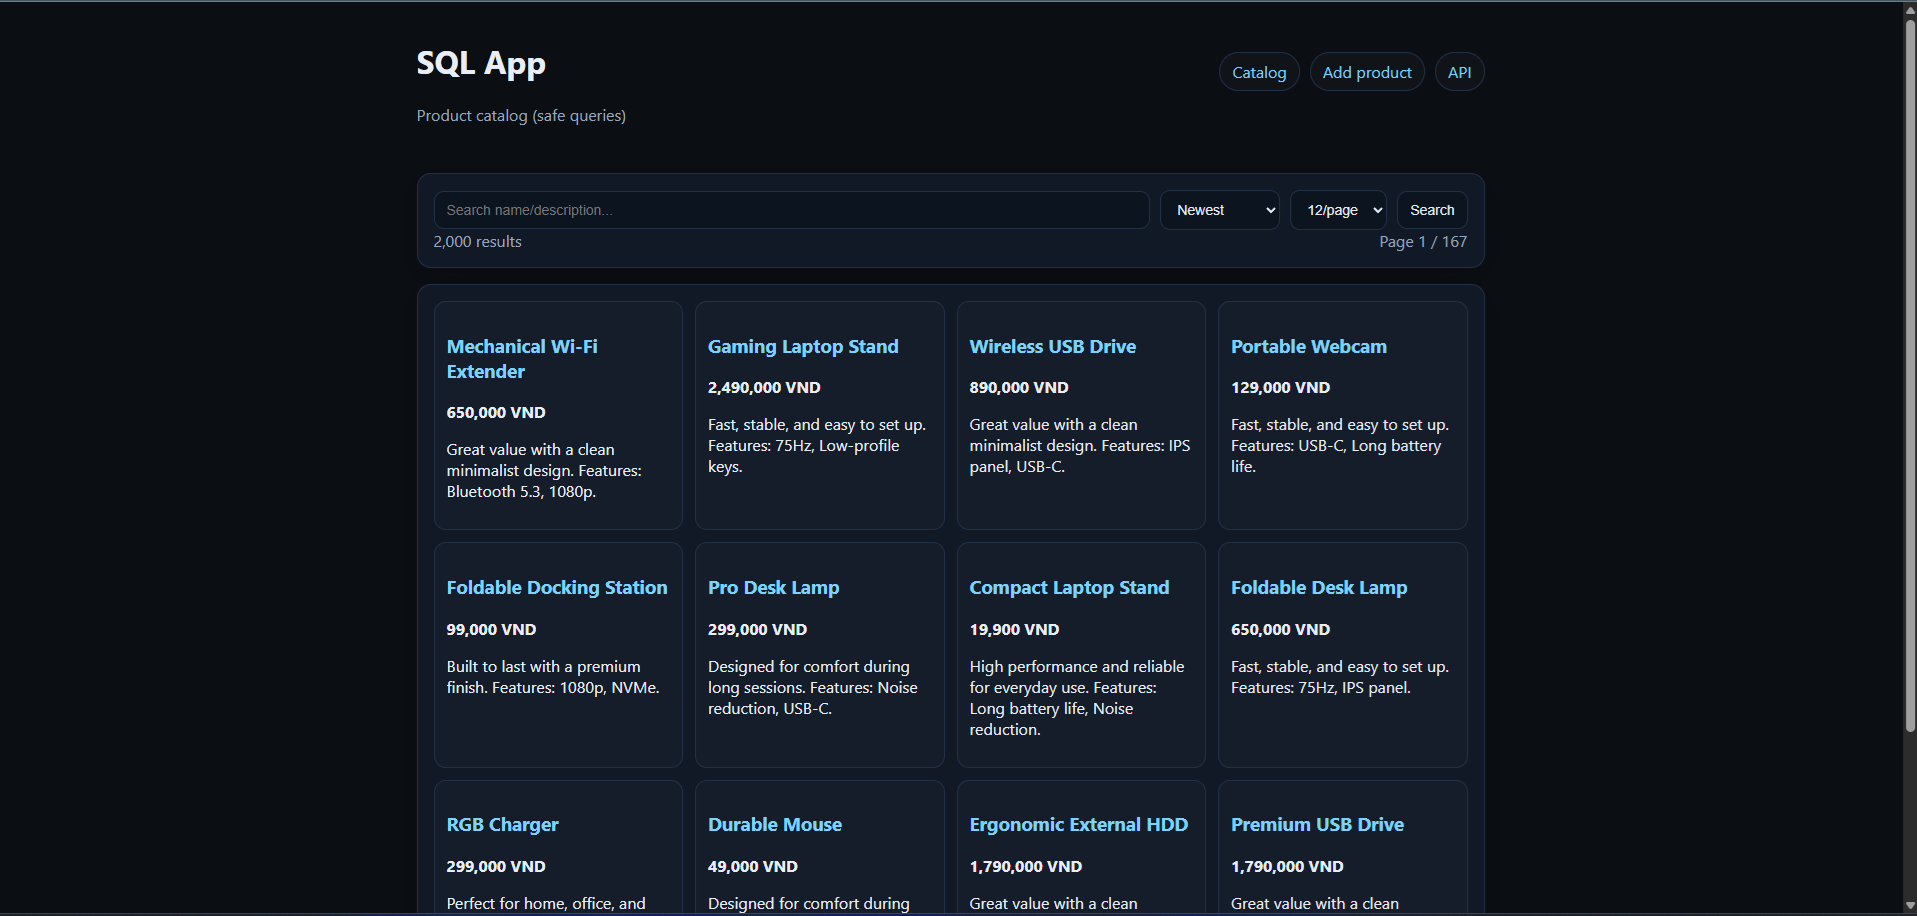
\includegraphics[width=0.92\textwidth]{images/cyred/cyred/2.png}
    \caption{SQL App target interface.}
    \label{fig:redteam-sqlapp-target}
\end{figure}

\subsubsection{Step 3: Connecting the Terminal to the Cyber Shell Assistant}
Before the assistant can reason over shell activity, the learner must connect the local terminal to the Cyber Shell service using the provided command. This step validates the telemetry bridge between terminal actions and the web dashboard. Once this connection is established, shell commands become visible in the assistant session and can later be used as context for AI responses.

\begin{figure}[H]
    \centering
    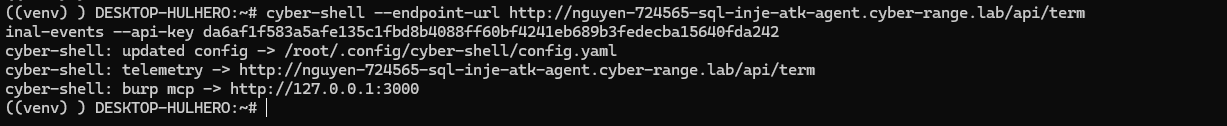
\includegraphics[width=0.92\textwidth]{images/cyred/cyred/3.png}
    \caption{Terminal connection to Cyber Shell.}
    \label{fig:redteam-terminal-connect}
\end{figure}

\subsubsection{Step 4: Verifying Session Synchronization on the Dashboard}
After terminal setup, the dashboard is checked to confirm that the new shell session and its recent commands are visible in the Cyber Shell Assistant interface. This validation step is important because the later AI guidance depends on accurate session awareness. The synchronized session history shows that the assistant can ground its responses in actual learner activity instead of relying only on manually typed prompts.

\begin{figure}[H]
    \centering
    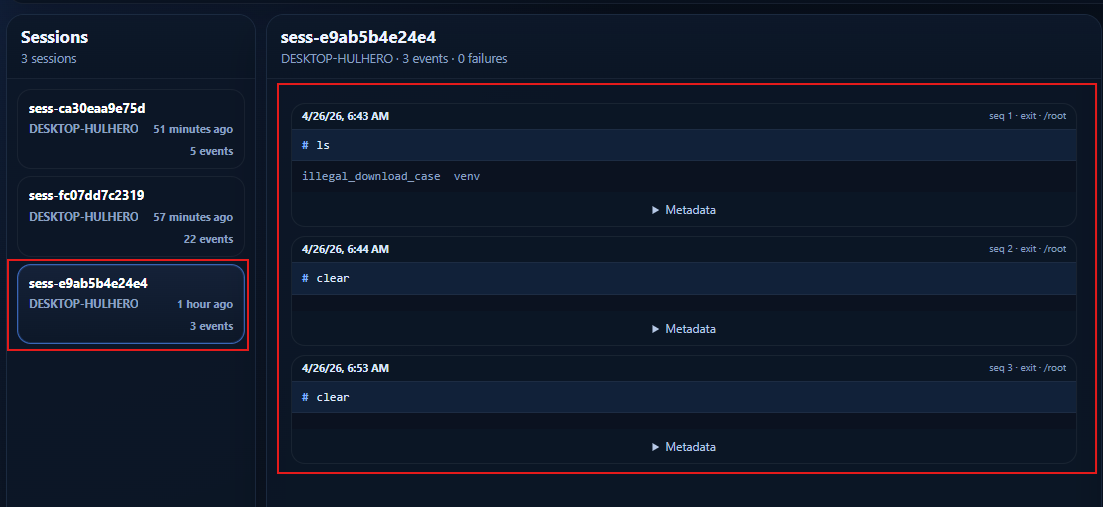
\includegraphics[width=0.92\textwidth]{images/cyred/cyred/4.png}
    \caption{Synchronized shell session in the dashboard.}
    \label{fig:redteam-session-sync}
\end{figure}

\subsubsection{Step 5: Probing the Target from the Terminal}
Once the session is active, the learner issues a direct \texttt{curl} request to the SQL App target. This step allows the assistant to observe which web target is being explored and also confirms that the target is reachable from the attack environment. The returned HTML output exposes the application structure and provides context for later exploitation steps.

\begin{figure}[H]
    \centering
    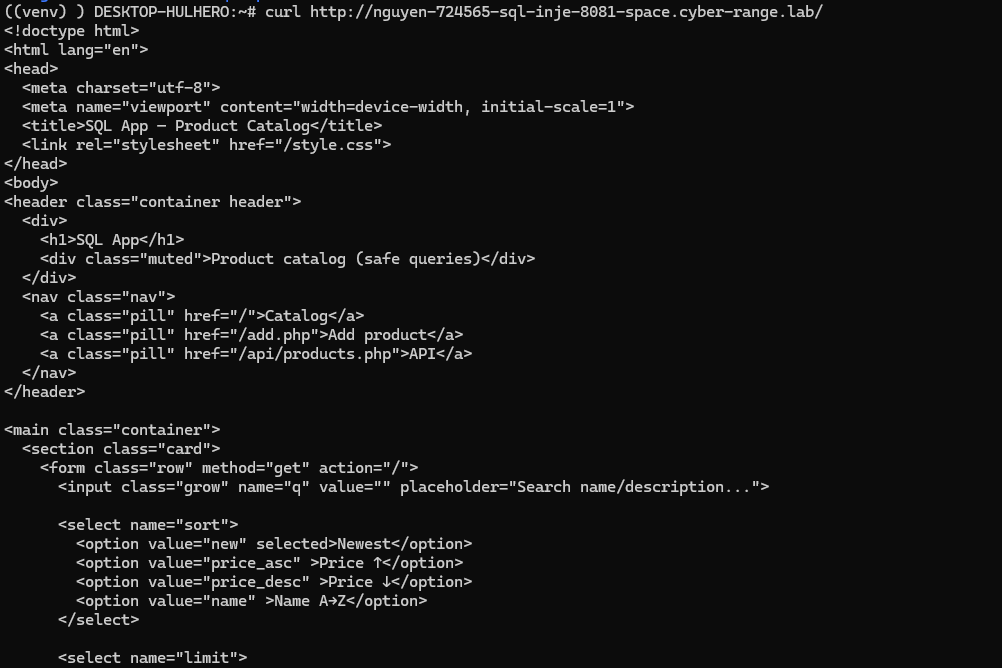
\includegraphics[width=0.92\textwidth]{images/cyred/cyred/5.png}
    \caption{Initial \texttt{curl} request to the target.}
    \label{fig:redteam-curl-target}
\end{figure}

\subsubsection{Step 6: Asking the Assistant to Identify the Target}
After the target is probed, the learner asks the Cyber Shell Assistant whether it can detect the website being targeted. The assistant answers using the recent shell history and demonstrates tool-assisted awareness by identifying the SQL App target and confirming that it can reach the application with an HTTP request. This step validates that the Red Team copilot is context-aware and can reason from captured terminal evidence.

\begin{figure}[H]
    \centering
    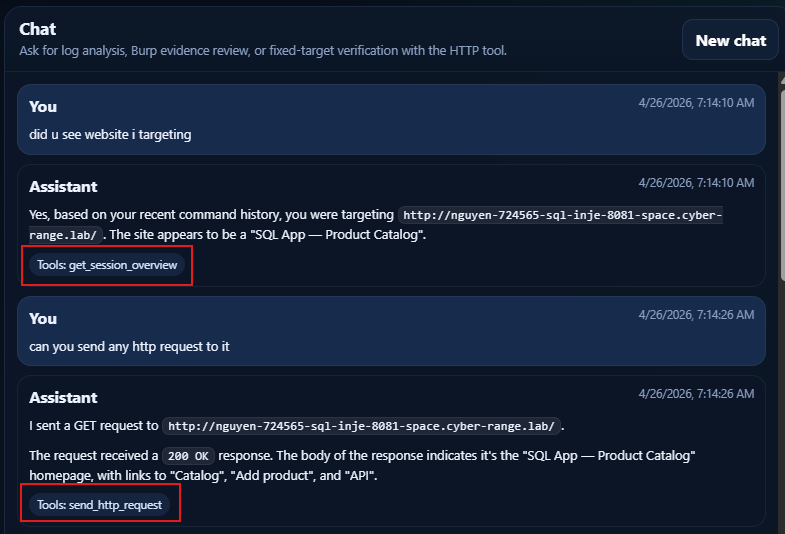
\includegraphics[width=0.92\textwidth]{images/cyred/cyred/6.png}
    \caption{Assistant identifies the target website.}
    \label{fig:redteam-assistant-identify-target}
\end{figure}

\subsubsection{Step 7: Requesting SQL Injection Guidance}
The next step validates AI-assisted offensive guidance. The learner asks how to check for SQL injection in the \texttt{q} URL parameter and how to use \texttt{sqlmap} to enumerate databases. The assistant responds with a command template that the learner can execute manually. This confirms that the assistant supports the learning process by suggesting relevant attack commands without directly carrying out the attack on its own.

\begin{figure}[H]
    \centering
    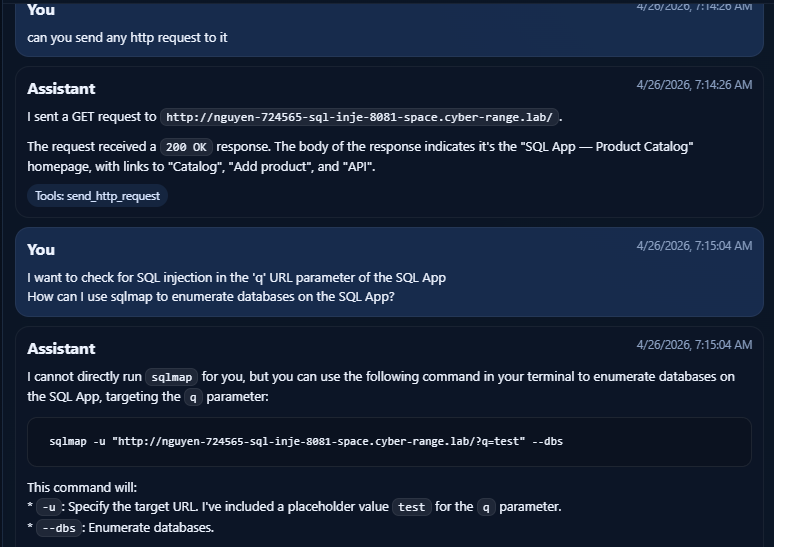
\includegraphics[width=0.92\textwidth]{images/cyred/cyred/7.png}
    \caption{Assistant guidance for SQL injection testing.}
    \label{fig:redteam-assistant-sqli-guidance}
\end{figure}

\subsubsection{Step 8: Enumerating Databases with \texttt{sqlmap}}
Following the assistant's suggestion, the learner executes the enumeration command in the terminal. The result shows that the backend DBMS is MySQL-compatible and that available databases include \texttt{information\_schema} and \texttt{shop\_db}. This step provides concrete exploitation evidence and validates that the guided command leads to a meaningful offensive result.

\begin{figure}[H]
    \centering
    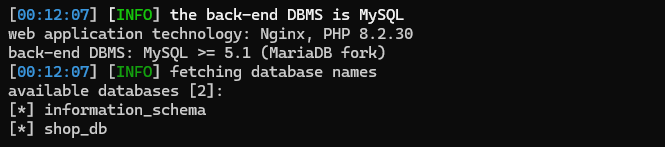
\includegraphics[width=0.92\textwidth]{images/cyred/cyred/8.png}
    \caption{Database enumeration with \texttt{sqlmap}.}
    \label{fig:redteam-sqlmap-dbs}
\end{figure}

\subsubsection{Step 9: Requesting Data-Dump Guidance}
After confirming the presence of the target database, the learner asks the assistant for a command to dump the data. The assistant returns a \texttt{sqlmap} command that targets \texttt{shop\_db} and uses the dump option. This step extends the earlier guidance from reconnaissance and enumeration toward data extraction and shows that the assistant can support multi-step offensive workflows.

\begin{figure}[H]
    \centering
    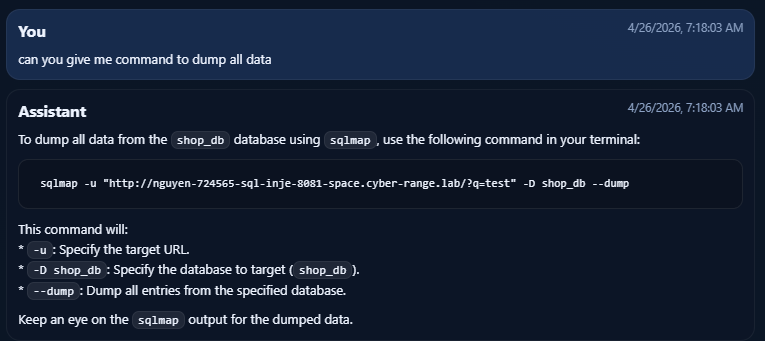
\includegraphics[width=0.92\textwidth]{images/cyred/cyred/9.png}
    \caption{Assistant guidance for dumping database content.}
    \label{fig:redteam-assistant-dump-guidance}
\end{figure}

\subsubsection{Step 10: Dumping Table Data from the Target Database}
In the final step, the learner executes the dump command and obtains table data from the \texttt{shop\_db} database. The terminal output shows fetched tables, columns, and product entries, demonstrating that the attack workflow progressed from target identification to database enumeration and then to data extraction. This final result validates the Red Team learning flow as an AI-assisted, session-aware attack exercise grounded in actual terminal interaction.

\begin{figure}[H]
    \centering
    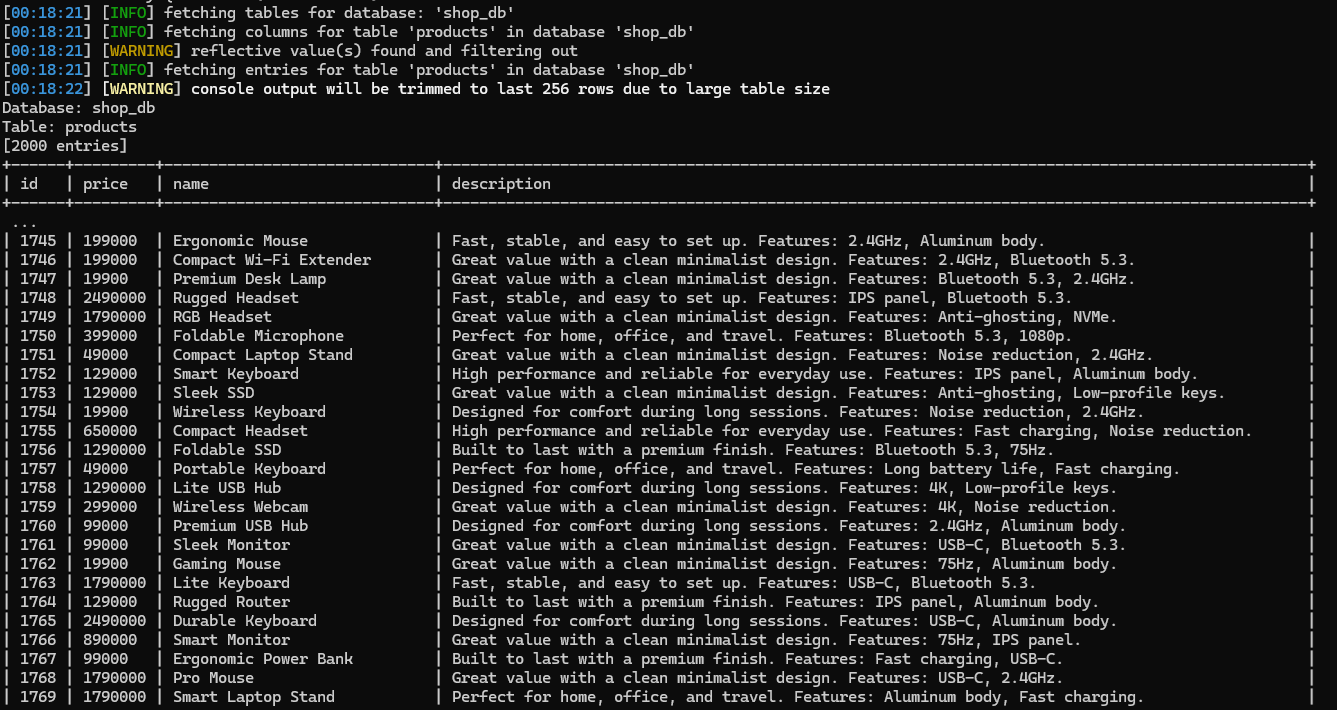
\includegraphics[width=0.92\textwidth]{images/cyred/cyred/10.png}
    \caption{Dumped data from \texttt{shop\_db}.}
    \label{fig:redteam-sqlmap-dump}
\end{figure}

Taken together, these ten steps validate a complete Red Team workflow: the learner accesses the Cyber Shell Assistant, connects the terminal, confirms session synchronization, probes the target, receives AI guidance, and executes offensive commands that enumerate and dump database content from the vulnerable web application. This evidence is especially valuable because it shows that the AI component supports hands-on offensive learning through contextual guidance rather than by replacing user action.


\subsection{RAG and No-RAG Benchmark Comparison}
A controlled benchmark was conducted to compare RAG and No-RAG on the same 800-request dataset. The comparison focuses on detection, attack intelligence, and grounded reasoning.

The results show that RAG is most valuable for semantic interpretation and grounded reasoning.

\subsubsection{Core Detection Performance}
Table~\ref{tab:core-detection-rag-vs-norag} summarizes the main detection metrics.

\begin{table}[H]
    \centering
    \small
    \setlength{\tabcolsep}{5pt}
    \renewcommand{\arraystretch}{1.15}
    \begin{tabularx}{\textwidth}{|X|c|c|c|}
        \hline
        \textbf{Metric} & \textbf{RAG} & \textbf{No-RAG} & \textbf{Observation} \\
        \hline
        Accuracy & 88.38\% & 88.38\% & Equivalent overall classification accuracy \\
        \hline
        Precision & 95.10\% & 93.80\% & RAG reduces false malicious predictions \\
        \hline
        F1-score & 93.23\% & 93.32\% & Comparable overall detection balance \\
        \hline
        Specificity & 67.00\% & 57.00\% & RAG better distinguishes benign traffic \\
        \hline
        False positive rate & 33.00\% & 43.00\% & RAG lowers benign misclassification \\
        \hline
    \end{tabularx}
    \caption{Core detection comparison.}
    \label{tab:core-detection-rag-vs-norag}
\end{table}

RAG keeps overall detection stable while improving precision and specificity.

The same tendency is visible in the overall comparison chart, where accuracy remains unchanged while precision and groundedness improve under the RAG setting.

\begin{figure}[H]
    \centering
    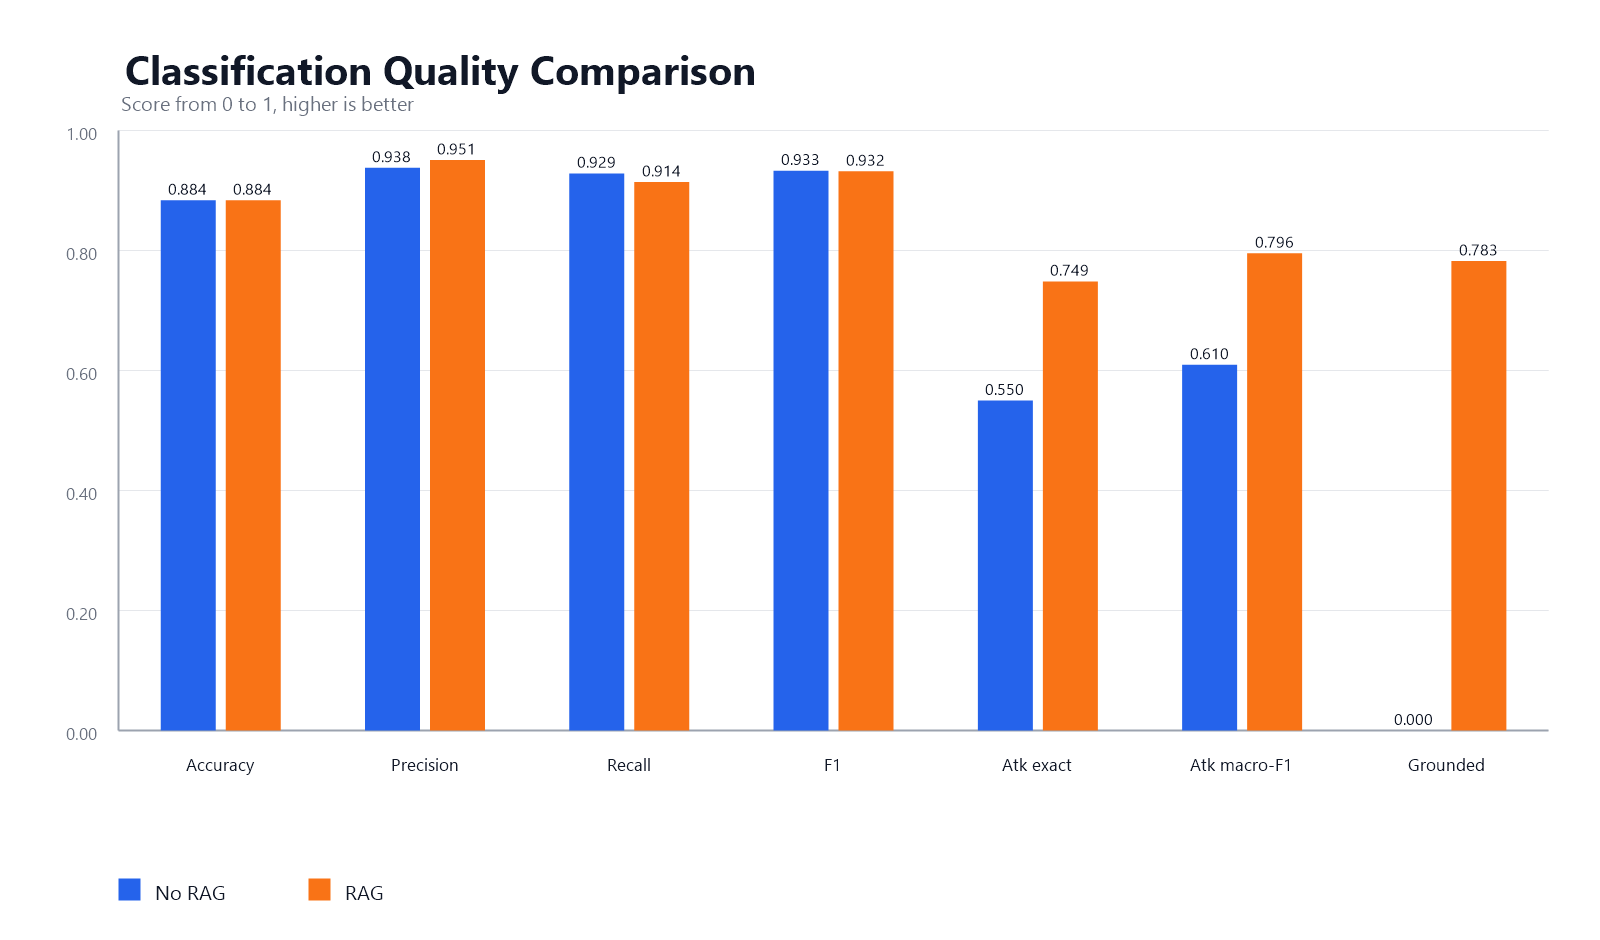
\includegraphics[width=0.95\textwidth]{images/chart_overall_comparison.png}
    \caption{Overall classification quality comparison.}
    \label{fig:rag-overall-comparison}
\end{figure}

\subsubsection{Attack-Intelligence Comparison}
The benchmark also measures how accurately the system identifies the attack family.

\begin{table}[H]
    \centering
    \small
    \setlength{\tabcolsep}{5pt}
    \renewcommand{\arraystretch}{1.15}
    \begin{tabularx}{\textwidth}{|X|c|c|c|}
        \hline
        \textbf{Metric} & \textbf{RAG} & \textbf{No-RAG} & \textbf{Observation} \\
        \hline
        Joint exact match accuracy & 74.86\% & 55.00\% & RAG strongly improves exact verdict+type correctness \\
        \hline
        Conditional exact match accuracy & 81.88\% & 59.23\% & RAG yields more accurate attack-family assignment \\
        \hline
        Macro-F1 for attack type & 79.55\% & 60.97\% & RAG improves balanced multi-class attack recognition \\
        \hline
    \end{tabularx}
    \caption{Attack-intelligence comparison.}
    \label{tab:attack-intelligence-rag-vs-norag}
\end{table}

RAG produces a clear improvement in attack-type intelligence.

This improvement is easier to observe in the per-attack visualization, where most attack families achieve a higher F1-score with RAG, especially SSI, LDAP Injection, SQL Injection, and XPath Injection.

\begin{figure}[H]
    \centering
    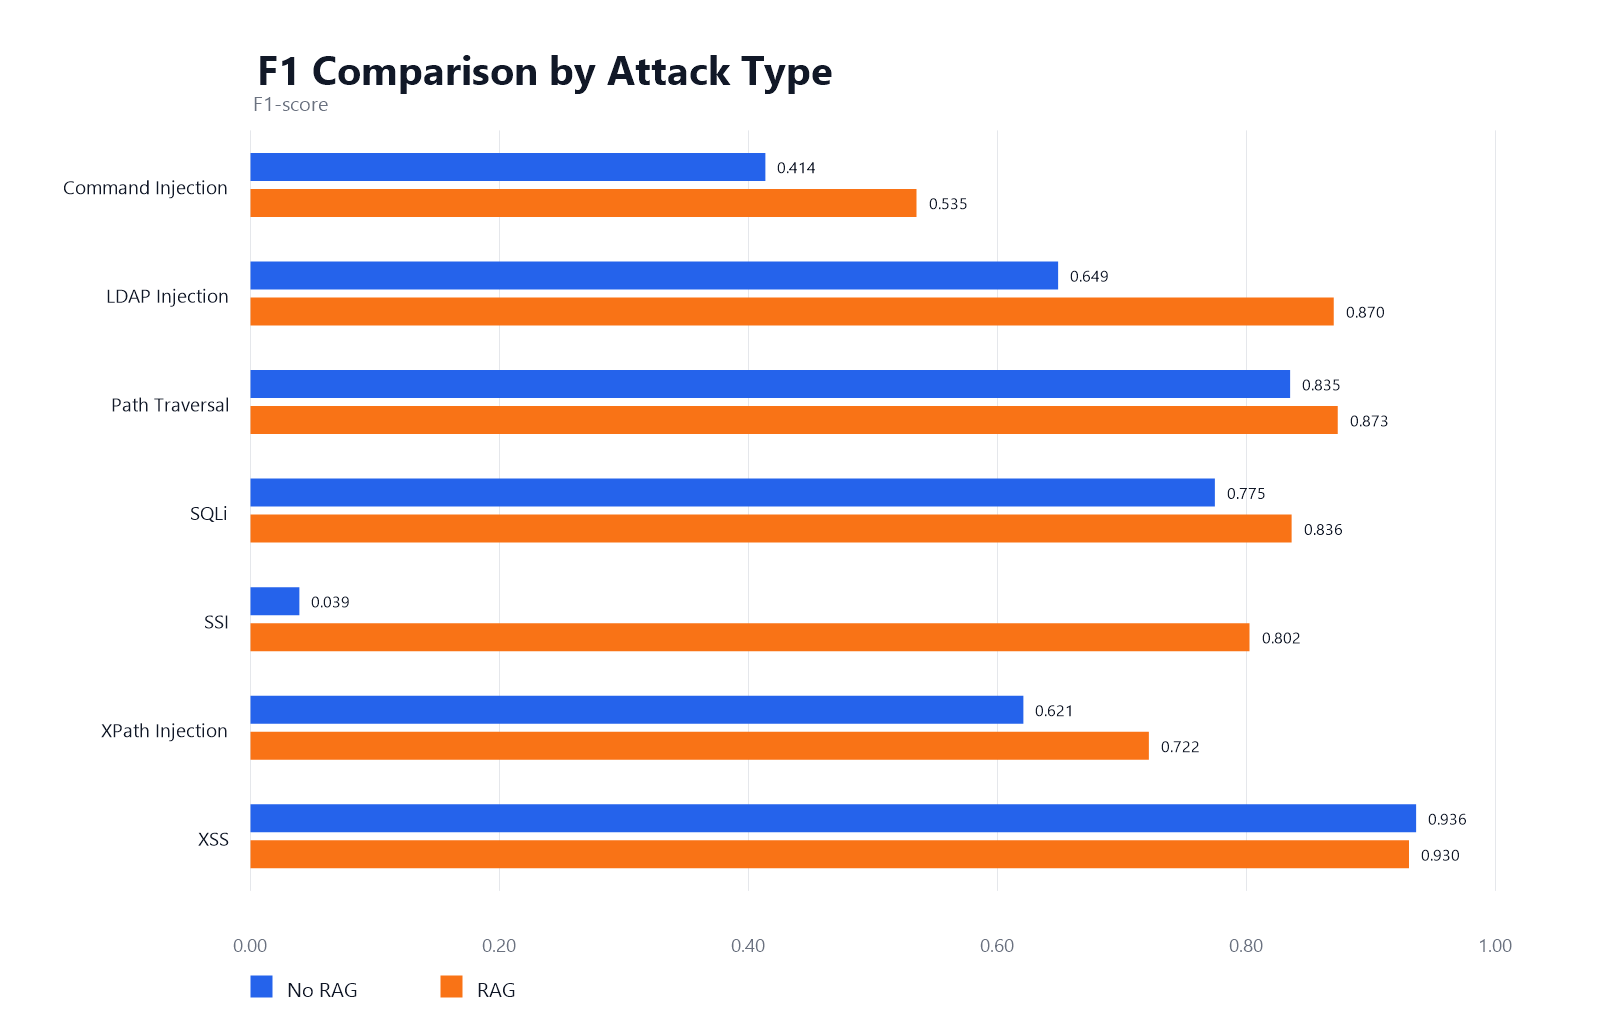
\includegraphics[width=0.95\textwidth]{images/chart_attack_type_f1_comparison.png}
    \caption{F1-score comparison by attack type.}
    \label{fig:rag-attack-type-f1}
\end{figure}

\subsubsection{Reasoning and Groundedness Comparison}
The final comparison evaluates whether LLM outputs remain evidence-grounded.

\begin{table}[H]
    \centering
    \small
    \setlength{\tabcolsep}{5pt}
    \renewcommand{\arraystretch}{1.15}
    \begin{tabularx}{\textwidth}{|X|c|c|c|}
        \hline
        \textbf{Metric} & \textbf{RAG} & \textbf{No-RAG} & \textbf{Observation} \\
        \hline
        LLM-path label accuracy & 91.79\% & 88.64\% & RAG improves verdict quality on LLM-routed samples \\
        \hline
        LLM-path attack-type accuracy & 89.86\% & 52.95\% & RAG greatly improves semantic interpretation \\
        \hline
        True attack type in top-k retrieval & 82.61\% & 0.00\% & Only RAG provides relevant retrieved support \\
        \hline
        Predicted attack type in top-k retrieval & 78.99\% & 0.00\% & RAG aligns generated output with retrieved context \\
        \hline
        Grounded correct rate & 78.26\% & 0.00\% & Grounded reasoning is only present with RAG \\
        \hline
        Eligible malicious LLM samples & 414 & 440 & Similar LLM-evaluated malicious volume \\
        \hline
    \end{tabularx}
    \caption{Reasoning and groundedness comparison.}
    \label{tab:groundedness-rag-vs-norag}
\end{table}

Overall, RAG mainly improves explanation quality, semantic accuracy, and groundedness.

\subsubsection{Latency Comparison}
The benchmark also considered the latency cost introduced by retrieval. As expected, the RAG pipeline is slower because it adds embedding, vector retrieval, and prompt augmentation before generation. However, the added latency remains acceptable for an academic cyber-range setting where explanation quality and grounded reasoning are more important than ultra-low response time.

\begin{figure}[H]
    \centering
    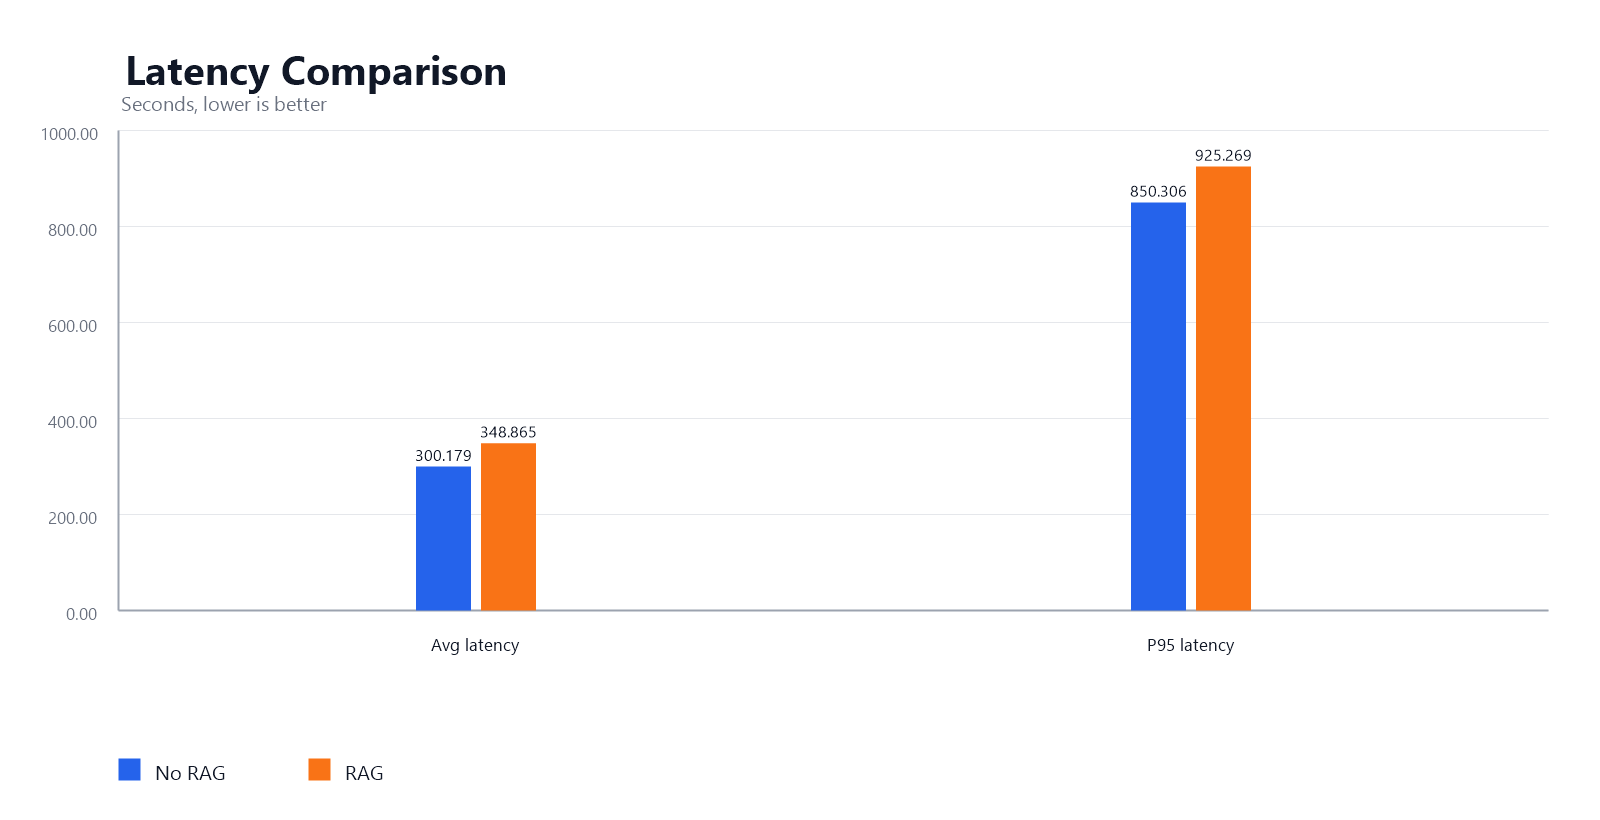
\includegraphics[width=0.95\textwidth]{images/chart_latency_comparison.png}
    \caption{Latency comparison between No-RAG and RAG.}
    \label{fig:rag-latency-comparison}
\end{figure}

In practical terms, the latency chart shows a moderate performance trade-off: RAG increases both average and tail latency, but the cost is accompanied by significantly better attack-type recognition and grounded output quality.

\section{Scope and Limitations}
This section clarifies the practical scope of the implemented system and the limits that should be considered when interpreting the validation results. The implemented system should be understood as an academic cyber-range platform with integrated orchestration and monitoring capabilities rather than a full enterprise production platform.

\subsection{Scope of Monitoring}
The current monitoring scope focuses on deployment lifecycle events, task/job status transitions, and operational logs generated by core workflow modules. The platform provides sufficient observability for academic scenario execution and validation, but does not yet claim full enterprise-grade telemetry breadth across heterogeneous production environments.

\subsection{Customization}
The platform supports practical customization for provider settings, reusable artifacts, scenario definitions, and dashboard-driven workflows. However, deep enterprise customization---such as complex multi-tenant policy abstraction or highly specialized governance templates---remains outside the present implementation scope.

\subsection{Risk Management Approach}
Risk management in the implemented system is iterative and control-oriented. The system reduces implementation risk through staged integration, checkpoint-based validation, and traceable asynchronous execution logs. This approach is effective for the capstone context but would require additional formalization for large-scale production governance.

\subsection{Ease of Use}
The dashboard is designed for guided academic usage, with module navigation aligned to the system lifecycle. The interface is suitable for technically oriented users and evaluators. Nevertheless, broader usability for mixed-skill user groups would benefit from additional onboarding aids, richer contextual help, and further UI refinement.

\subsection{Reporting and Visualization}
The reporting and visualization layer provides operationally useful views for configuration status, scenario progress, and task outcomes. These views are appropriate for validation and educational demonstration. Advanced analytical reporting and long-horizon operational intelligence remain future enhancement areas.

\section{Future Development}
Future development should expand both capability depth and deployment robustness. Priority directions include broader scenario libraries, stronger automation of repeated validation workflows, and improved fault recovery in asynchronous execution paths. Additional UI/UX refinement should focus on guided interaction, clearer error interpretation, and reduced operational friction for new users.

Scalability-oriented improvements should target multi-user concurrency handling, resource governance, and stronger isolation-aware orchestration for higher usage loads. AI-assisted support can be extended through better contextual integration, response consistency controls, and training-oriented feedback design.

Together, these improvements would move the platform beyond its current academic baseline toward a more mature cyber-range system with stronger multi-user readiness and richer analytical support.
	% !TeX root = ../main.tex
\chapter*{REFERENCES}
\addcontentsline{toc}{chapter}{REFERENCES}

\begin{enumerate}

\item
M. Fateh, T. T. T. Nguyen, S. George, and H. Hacid.
\textbf{Source type:} Journal article / cybersecurity education research.
\textit{Leveraging LLMs for generation and evaluation of cybersecurity training scenarios: a case study of phishing attack simulations},
International Journal of Information Security, 2025.
Available: \url{https://link.springer.com/article/10.1007/s44427-025-00006-3}.

\item
J. Molina, T. Stengel, and S. Eickhoff.
\textbf{Source type:} Preprint / LLM security analysis research.
\textit{Prompt Injection Detection with Hidden-Markov Models},
arXiv preprint, 2024.
Available: \url{https://arxiv.org/abs/2412.01421}.

\item
P. M. Nell, A. M. Trindade, C. M. Junqueira, A. C. B. Garcia, and C. M. N. dos Santos.
\textbf{Source type:} Preprint / RAG evaluation research.
\textit{ERA: Evaluating RAG with LLMs as Judges in Incident Postmortems},
arXiv preprint, 2026.
Available: \url{https://arxiv.org/abs/2604.20854}.

\item
J. Hu, X. Wen, and L. Wang.
\textbf{Source type:} Preprint / adversarial testing of LLM agents.
\textit{R-Bench: Benchmarking and Enhancing Robustness in LLM-Based Multi-Agent Systems},
arXiv preprint, 2026.
Available: \url{https://arxiv.org/abs/2604.20598}.

\item
R. Prabhakar, R. Tanna, and A. N. Srivastava.
\textbf{Source type:} Preprint / cyber threat intelligence with retrieval research.
\textit{RARE: Retrieval-Augmented Reasoning and Extraction for Cyber Threat Intelligence from IOC Reports},
arXiv preprint, 2026.
Available: \url{https://arxiv.org/abs/2604.19047}.

\item
V. Mazzi, I. Gandin, M. Pavan, and F. Silvestri.
\textbf{Source type:} Preprint / context-aware retrieval research.
\textit{Context-Aware Search on Documentation Graphs for Enhanced Code Generation},
arXiv preprint, 2026.
Available: \url{https://arxiv.org/abs/2604.18424}.

\item
S. Li, Z. Huang, Y. Zhang, Z. Tan, W. Liang, and D. Tao.
\textbf{Source type:} Preprint / reasoning benchmark research.
\textit{Evaluating Multi-Hop Reasoning in Large Language Models via Open-Domain Information-Seeking Questions},
arXiv preprint, 2026.
Available: \url{https://arxiv.org/abs/2604.18234}.

\item
OWASP Foundation.
\textbf{Source type:} Security standard / industry guidance.
\textit{OWASP Top 10: The Ten Most Critical Web Application Security Risks},
2021.
Available: \url{https://owasp.org/Top10/}.

\item
National Institute of Standards and Technology (NIST).
\textbf{Source type:} Government standard / technical guideline.
\textit{Security and Privacy Controls for Information Systems and Organizations (SP 800-53 Rev. 5)},
2020.
Available: \url{https://csrc.nist.gov/pubs/sp/800/53/r5/final}.

\item
MITRE.
\textbf{Source type:} Threat intelligence knowledge base / framework documentation.
\textit{MITRE ATT\&CK Framework},
Available: \url{https://attack.mitre.org/}.

\item
Proxmox Server Solutions GmbH.
\textbf{Source type:} Virtualization platform documentation.
\textit{Proxmox Virtual Environment Documentation},
Available: \url{https://pve.proxmox.com/pve-docs/}.

\item
Wazuh Inc.
\textbf{Source type:} SIEM platform documentation.
\textit{Wazuh Documentation},
Available: \url{https://documentation.wazuh.com/}.

\item
Docker Inc.
\textbf{Source type:} Container platform documentation.
\textit{Docker Documentation},
Available: \url{https://docs.docker.com/}.

\item
HashiCorp.
\textbf{Source type:} Infrastructure automation documentation.
\textit{Packer Documentation},
Available: \url{https://developer.hashicorp.com/packer/docs}.

\item
Ansible Project.
\textbf{Source type:} Automation framework documentation.
\textit{Ansible Documentation},
Available: \url{https://docs.ansible.com/}.

\item
FastAPI.
\textbf{Source type:} Backend framework documentation.
\textit{FastAPI Documentation},
Available: \url{https://fastapi.tiangolo.com/}.

\item
LangChain Inc.
\textbf{Source type:} LLM orchestration framework documentation.
\textit{LangGraph Documentation},
Available: \url{https://langchain-ai.github.io/langgraph/}.

\item
Qdrant.
\textbf{Source type:} Vector database documentation.
\textit{Qdrant Documentation},
Available: \url{https://qdrant.tech/documentation/}.

\item
VMware, Inc.
\textbf{Source type:} Message broker documentation.
\textit{RabbitMQ Documentation},
Available: \url{https://www.rabbitmq.com/docs}.

\item
Celery Project.
\textbf{Source type:} Distributed task queue documentation.
\textit{Celery Documentation},
Available: \url{https://docs.celeryq.dev/}.

\item
Redis Ltd.
\textbf{Source type:} In-memory data store documentation.
\textit{Redis Documentation},
Available: \url{https://redis.io/docs/}.

\item
The PostgreSQL Global Development Group.
\textbf{Source type:} Relational database documentation.
\textit{PostgreSQL Documentation},
Available: \url{https://www.postgresql.org/docs/}.

\item
Traefik Labs.
\textbf{Source type:} Reverse proxy documentation.
\textit{Traefik Proxy Documentation},
Available: \url{https://doc.traefik.io/traefik/}.

\item
Apache Software Foundation.
\textbf{Source type:} Remote access gateway documentation.
\textit{Apache Guacamole Documentation}.
Available: \url{https://guacamole.apache.org/doc/}.

\item
F5, Inc.
\textbf{Source type:} Web server / reverse proxy documentation.
\textit{NGINX Documentation},
Available: \url{https://docs.nginx.com/}.

\item
OWASP Foundation.
\textbf{Source type:} Web application firewall ruleset documentation.
\textit{ModSecurity Core Rule Set (CRS) Documentation},
Available: \url{https://coreruleset.org/docs/}.

\item
Google.
\textbf{Source type:} API documentation / LLM service documentation.
\textit{Gemini API Documentation},
Available: \url{https://ai.google.dev/gemini-api/docs}.

\end{enumerate}
\end{document}